%\documentclass[12pt]{report}
\documentclass[11pt,english]{scrbook}
%% LyX 2.3.1-1 created this file.  For more info, see http://www.lyx.org/.
%% Do not edit unless you really know what you are doing.
\usepackage{newcent}
\usepackage{helvet}
\usepackage{courier}
\renewcommand{\familydefault}{\rmdefault}
\usepackage[T1]{fontenc}
\usepackage[latin9]{inputenc}
\usepackage[a4paper]{geometry}
\geometry{verbose,tmargin=2.5cm,bmargin=2.5cm,lmargin=2cm,rmargin=2cm}
\setcounter{secnumdepth}{3}
\usepackage{color}
\usepackage{babel}
\usepackage{enumitem}
\usepackage{amsmath}
\usepackage{amsthm}
\usepackage{amssymb}
\usepackage{makeidx}
\makeindex
\usepackage{graphicx}
\usepackage{subfigure}
\usepackage{setspace}
\usepackage{nomencl}
\usepackage{acronym} 
% the following is useful when we have the old nomencl.sty package
%\providecommand{\printnomenclature}{\printglossary}
%\providecommand{\makenomenclature}{\makeglossary}
%\makenomenclature
\usepackage[unicode=true,pdfusetitle,
 bookmarks=true,bookmarksnumbered=true,bookmarksopen=false,
 breaklinks=false,pdfborder={0 0 0},pdfborderstyle={},backref=false,colorlinks=true]
 {hyperref}

\makeatletter
%%%%%%%%%%%%%%%%%%%%%%%%%%%%%% Textclass specific LaTeX commands.
%\numberwithin{equation}{section}
%\numberwithin{figure}{section}
\newlist{casenv}{enumerate}{4}
\setlist[casenv]{leftmargin=*,align=left,widest={iiii}}
\setlist[casenv,1]{label={{\itshape\ \casename} \arabic*.},ref=\arabic*}
\setlist[casenv,2]{label={{\itshape\ \casename} \roman*.},ref=\roman*}
\setlist[casenv,3]{label={{\itshape\ \casename\ \alph*.}},ref=\alph*}
\setlist[casenv,4]{label={{\itshape\ \casename} \arabic*.},ref=\arabic*}
\theoremstyle{plain}
\newtheorem{thm}{\protect\theoremname}
\theoremstyle{definition}
\newtheorem{defn}[thm]{\protect\definitionname}

%%%%%%%%%%%%%%%%%%%%%%%%%%%%%% User specified LaTeX commands.
\usepackage{multicol} %For multiple columns
\usepackage{mathptmx} % For times new roman font
\usepackage{lscape} %For Putting a picture on whole page in landscape mode
\usepackage{setspace}
\usepackage{enotez}
\usepackage{array}
\usepackage{wrapfig}
\renewcommand{\nomname}{Glossary of Symbols \& Terms}
\usepackage{lettrine} %For Dropcaps
\renewcommand{\qedsymbol}{$\blacksquare$}
\usepackage{scrextend}
\newcolumntype{D}[1]{>{\let\newline\\\arraybackslash\hspace{0pt}}m{#1}} 
\newcolumntype{C}[1]{>{\centering\let\newline\\\arraybackslash\hspace{0pt}}m{#1}}
%\usepackage[font=sf]{caption}
\let\footnote=\endnote
\setenotez{
  reset = true ,
  list-heading = \section*{#1}
}
\newcommand\Fontvii{\fontsize{6}{7.2}\selectfont}

%%%%%%%% rverma %%%%%%%%%%%%%
%\newcommand{\pt}{pT }
%\newcommand{\pt}{$p_{T}$}
%\newcommand{\unit}[1]{\textrm{#1}}
%\newcommand{\MET}{$E_{T}^{miss}$ }
\renewcommand{\bf}{\textbf}
\renewcommand{\it}{\textit}
\renewcommand{\rm}{\textrm}
\renewcommand{\arraystretch}{1.2}
\newcommand{\quotes}[1]{``#1''}
\newcommand{\dq}{\quotes}
\usepackage[toc,page]{appendix}
\usepackage{adjustbox}
%%%%%%%%%%%%%%%%%%%%%%%%%%%%%%%%

%%---------------------------------
%CERN-LHC-CMS specific
%%---------------------------------
\RequirePackage{ptdr-definitions}
\RequirePackage{changepage}
\RequirePackage{heppennames2}
\RequirePackage{hypernat}
\RequirePackage{maybemath}
\RequirePackage{pdfdraftcopy}
\RequirePackage{placeins}
\RequirePackage{topcapt}
\newcommand{\Hp}{\ensuremath{\PH^+}\xspace}
\newcommand{\Hn}{\ensuremath{\PH^-}\xspace}
\newcommand{\ttjets}{\ensuremath{\ttbar + \text{jets}}\xspace}
\newcommand{\wjets}{\ensuremath{\PW + \text{jets}}\xspace}
\newcommand{\dyjets}{\ensuremath{\PZ/\PGg + \text{jets}}\xspace}
\newcommand{\mjj}{\ensuremath{m_\text{jj}}\xspace}
\newcommand{\mt}{\ensuremath{m_{\PQt}}\xspace}
\newcommand{\mujets}{\ensuremath{\mu + \text{jets}}\xspace}
\newcommand{\ejets}{\ensuremath{\text{e} + \text{jets}}\xspace}
\newcommand{\ljets}{\ensuremath{\text{l} + \text{jets}}\xspace}

\newcommand{\mHp}{\ensuremath{m_{\text{H}^+}}\xspace}
\newcommand{\brHcs}{\ensuremath{\mathcal{B}(\text{H}^+ \rightarrow \text{c}\bar{\text{s}})}\xspace}
\newcommand{\brHtv}{\ensuremath{\mathcal{B}(\text{H}^+ \rightarrow \tau^+\nu_\tau)}\xspace}
\newcommand{\brThb}{\ensuremath{\mathcal{B}(\text{t} \rightarrow \text{H}^+ \text{b})}\xspace}
\newcommand{\brTwb}{\ensuremath{\mathcal{B}(\text{t} \rightarrow \text{W}^+ \text{b})}\xspace}
\newcommand{\brTwq}{\ensuremath{\mathcal{B}(\text{t} \rightarrow \text{W}^+ \text{q})}\xspace}
\newcommand{\sigHp}{\ensuremath{\sigma(\text{pp} \rightarrow \text{t} \text{H}^+ + \text{X})}\xspace}

\usepackage{cite}
\@ifundefined{showcaptionsetup}{}{%
 \PassOptionsToPackage{caption=false}{subfig}}
%\usepackage{subfig}
\makeatother

\providecommand{\casename}{Case}
\providecommand{\definitionname}{Definition}
\providecommand{\theoremname}{Theorem}


%%%%%%%%% to include publications %%%%%%%%
\usepackage{textcomp} % text version of symbols in TS1, e.g. \textrightarrow{}
\usepackage{amstext} % proper support of frequently used \text{} command
\newif\ifshowcitations\showcitationsfalse%
\newif\ifshowlinks\showlinksfalse%
\ifshowlinks%
  \usepackage[
         colorlinks=true,
         urlcolor=blue,       % \href{...}{...} external (URL)
         ]{hyperref}
  \newcommand*{\inspireurl}[1]{\\\href{#1}{INSPIRE-HEP entry}}
\else
  \makeatletter
  \newcommand*{\inspireurl}[1]{\@bsphack\@esphack}
  \makeatother
\fi
\ifshowcitations%
  \newcommand*{\citations}[1]{\\* #1}
\else
  \makeatletter
  \newcommand*{\citations}[1]{\@bsphack\@esphack}
  \makeatother
\fi
\renewcommand{\labelenumii}{\arabic{enumi}.\arabic{enumii}}

%%% to remove bullet points
%\usepackage{enumitem}
%{\renewcommand\labelitemi{}
%\setlength{\cftfigurenumwidth}{5em}
\makeatletter
\renewcommand{\l@figure}{\@dottedtocline{1}{1.5em}{2.3em}}
\makeatother

\usepackage{fancyheadings}
\pagestyle{fancy}
%\pagestyle{fancyplain}
%\renewcommand{\chaptermark}[1]{\markboth{#1}{}}
%\renewcommand{\sectionmark}[1]{\markleft{\thesection\ #1}}
%\renewcommand{\sectionmark}[1]{\markright{\thesection\ #1}}
\lhead[\fancyplain{}{\thepage}]
{\fancyplain{}{\rightmark}}
\rhead[\fancyplain{}{\leftmark}]
{\fancyplain{}{\thepage}}
\cfoot{}
\cfoot[\fancyplain{\rm\thepage}{}]{\fancyplain{\rm\thepage}{}}
\pagenumbering{arabic}

%\oddsidemargin 0.0in
\textwidth 6.5in
%\topmargin -0.75in
%\topmargin 2.5cm
%\bottommargin 2.5cm
\textheight 9.0in
%\textheight 9.5in

\usepackage{titlesec, blindtext, color}
\definecolor{gray75}{gray}{0.75}
\newcommand{\hsp}{\hspace{20pt}}
\titleformat{\chapter}[hang]{\Huge\bfseries}{\thechapter\hsp\textcolor{gray75}{|}\hsp}{0pt}{\Huge\bfseries}

%%%%%%%%%%\oddsidemargin +0.4 cm
\flushbottom
%\textheight 21cm
%\renewcommand{\familydefault}{\sfdefault}

%\linespread{1.5}
\begin{document}
%%-----------------------------------
%% University specifics
%%-----------------------------------

\baselineskip 20pt
\abovedisplayskip=0mm
\belowdisplayskip=5mm
\abovedisplayshortskip=0mm
\belowdisplayskip=5mm
\abovedisplayshortskip=0mm
\belowdisplayshortskip=5mm
\parskip=0.25cm

\pagestyle{plain}
\begin{singlespace}
\begin{titlepage} 
\begin{center}
{\Huge\textsc {Search for a charged Higgs Boson at 13 TeV in the CMS experiment at the LHC, CERN}
\\[.5in]} 
{\large \textit{A thesis submitted}\\[0.1in] in partial fulfilment of the requirement\\[0.1in] for the Degree of\\[0.1in] \textsc{ Doctor of Philosophy}\\[0.5in]}
by\\ {\large \textbf{\textsc{Ravindra Kumar Verma} (13109883)}}\\[0.9in]

\includegraphics[scale=0.50]{University/Image/IIT_Kanpur_Logo}\\[0.9in]
{\Large \textsc{to} \\ \textsc{The Department of Physics}\\\textsc{Indian Institute of
	Technology, Kanpur, India}\\[.5in]}
{\Large \textsc{August} 2019}
\end{center}
\end{titlepage} 
\end{singlespace}


\frontmatter
\chapter{Certificate}
It is certified that the work contained in the thesis titled 
``\textsc{Search for a charged Higgs Boson at 13 TeV in the CMS experiment at the LHC, CERN}'' by 
\rm{Ravindra Kumar Verma} has been carried out under our supervision and this work has not been submitted elsewhere for a degree.

\vspace{3cm}
\begin{flushright}
\textsc{Prof Pankaj Jain}

\textsc{Supervisor}

\textsc{Department of Physics}

\textsc{IIT Kanpur}
\end{flushright} 

\vspace{3cm}
\begin{flushright}
\textsc{Prof Shashi R Dugad}

\textsc{Co-supervisor}

\textsc{Department of High Energy Physics}

\textsc{TIFR Mumbai}
\end{flushright} 

\textsc{August 2019}

%\chapter{\centerline{\Huge\textbf{ Synopsis}}}
\chapter{Synopsis}
\bigskip
\begin{quote}
\begin{tabular}[c]{ll}
Name: & {\textbf {Ravindra Kumar Verma}}\\
Roll No.: & {\textbf{ 13109883}}\\
Degree for which submitted: &  {\textbf{ Doctor of Philosophy}}\\
Department: & {\textbf{ Physics}}\\
Thesis Title: & {\textbf{ Search for a charged Higgs Boson at 13 TeV }}\\
 {}& {\textbf{ in the CMS experiment at the LHC, CERN}}\\
Thesis Supervisors: & {\textbf{ Prof. Pankaj Jain (IIT Kanpur),}}\\ 
{}&{\textbf{ Prof. Shashi R. Dugad (TIFR Mumbai)}}\\ 
Month and year of submission: & {\textbf{ August 2019}} 
\end{tabular}
\end{quote}
\hrulefill
\bigskip

The discovery of the Higgs boson in 2012 by the ATLAS and CMS experiments at 
the CERN LHC has ushered a new beginning in the field of particle physics. 
The Higgs boson could be the first of many elementary scalars present in 
nature to be observed in the laboratory. Various extensions to the standard 
model (SM), such as supersymmetry and the two Higgs doublet model (2HDM), 
predict multiple scalars as the remnants of an additional SU(2)$_L$ complex 
doublet introduced to address some known drawbacks of the SM. After spontaneous 
symmetry breaking, out of the eight degrees of freedom of the two Higgs doublets, 
three are used to make the \PW and \PZ bosons massive, leaving five physical scalar
particles. Of these, two (\Ph, \PH) are neutral Higgs bosons which are
CP-even (scalar), one (\PSA) is neutral and CP-odd (pseudoscalar), and the
remaining two are charged Higgs \PHpm bosons.

The 2HDM can be classified into different categories depending on the type of
interaction of the two doublets with quarks and charged leptons. For example,
in the type I 2HDM, fermions have Yukawa couplings only to the second doublet.
The nature of the Yukawa coupling determines the branching fraction of the charged
Higgs boson decays into different final states. In this thesis, a search for the
charged Higgs boson has been performed in the decay channel $\Hp \to \PQc\PAQs$ (and 
its charge conjugate), whose branching fraction 
can range anywhere up to 100\% depending on the type of Yukawa couplings. The 
latter is expressed in terms of the parameter $\tan\beta=v_2/v_1$ where $v_1$ 
and $v_2$ are the vacuum expectation values of the two Higgs doublets. In the 
minimal supersymmetric standard model (MSSM), this is the dominant decay channel 
for low values of $\tan\beta$. In this thesis, we perform a model-independent search for the charged Higgs boson assuming that $\mathcal{B}(\Hp \to \PQc\PAQs) = 100$\%. 

Limits on charged Higgs boson production at hadron colliders have been set by the 
Tevatron and LHC, assuming the production mode $\PQt \to \Hp\PQb$. The CDF 
collaboration set a 95\% \CL upper limit on the branching 
fraction $\mathcal{B}(\PQt \to \Hp\PQb) < 10$--30\% for a charged Higgs lying in 
the mass range 60--150\GeV, assuming that $\Hp$ decays dominantly to $\PQc\PAQs$. 
Similar limits have been obtained by the D0 experiment. 
Using the 7\TeV data, the ATLAS collaboration set an upper limit at 95\% \CL on 
the product $\mathcal{B}(\PQt \to \Hp\PQb) \mathcal{B}(\Hp \to \PGtp\PGn) < 
0.23$--1.3\% for a charged Higgs mass in the range 80--160\GeV. 
A search for a charged Higgs boson decaying into $\PQc\PAQs$ was performed at 
8\TeV by the CMS collaboration, which set an upper limit at 95\% \CL on 
$\mathcal{B}(\PQt \to \Hp\PQb)$ in the range 1.2--6.5\%. In this thesis, 
the analysis of collision data recorded in 2016 by the CMS experiment at 13\TeV
is presented.  

As illustrated in Figure~\ref{fig:feyn_diag_sig}, the principal SM background to 
this search consists of \ttbar pair production where one of the top quarks decays 
by $\PQt \to \PWp\PQb$ and the other top quark decays by $\PAQt \to \PWm\PAQb$; 
this is referred to as the \dq{semileptonic} decay channel. In contrast, in the signal
process, one of the top quarks decays to $\Hp\PQb$ and the other to $\PWm\PAQb$. 
The $\PWp/\Hp$ decays hadronically into \dq{light} jets (not from a \PQb quark), 
whereas the \PWm decays leptonically. We define two channels depending on whether 
the lepton produced in the \PWm decay is an electron or a muon (events with tau 
leptons are not considered).
\begin{figure}[htp]
\begin{center}
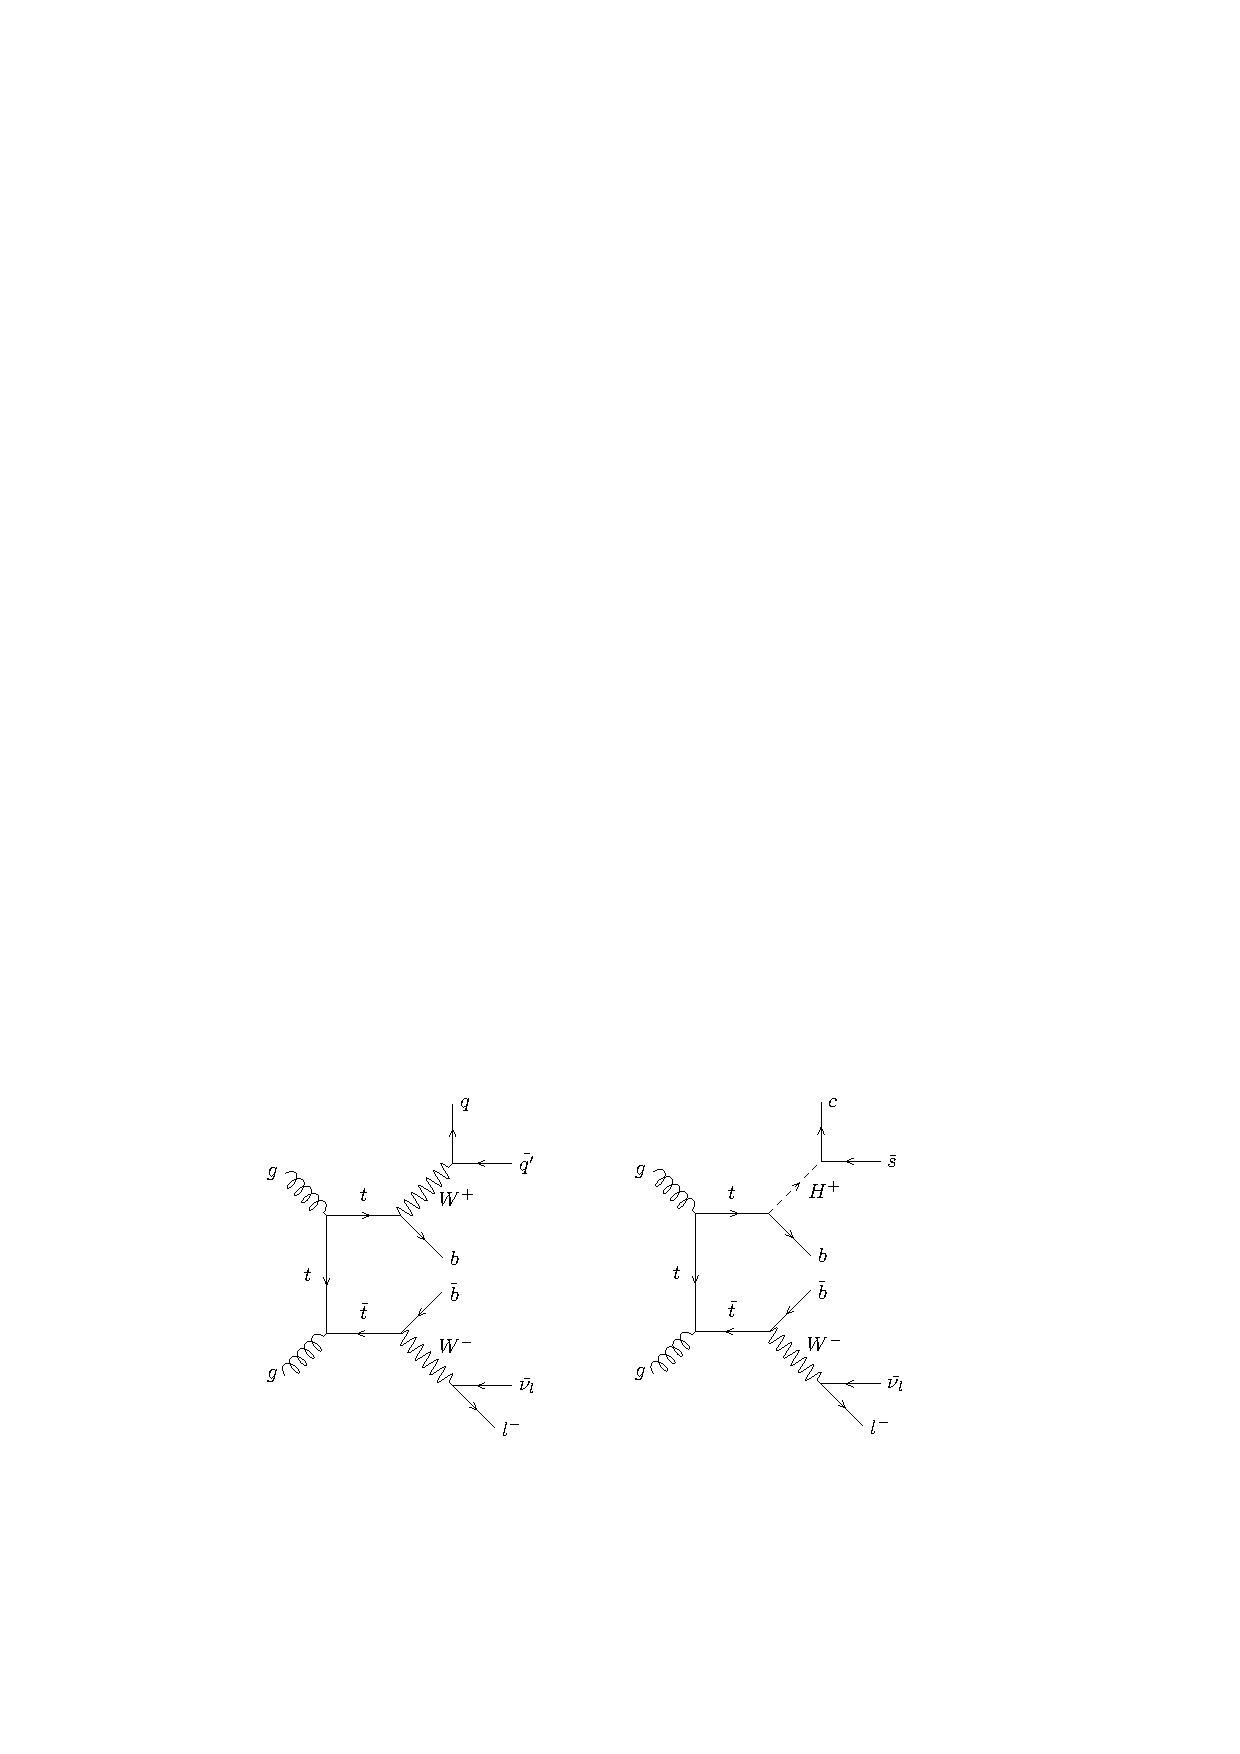
\includegraphics[width=0.75\textwidth]{University/Image/Synopsis/feyn_diag_sig.pdf}
\caption{Production of \ttbar from gluon-gluon scattering. The left plot shows
the SM decay of the \ttbar pair in the semileptonic decay channel. The right plot 
shows the signal process in which the \ttbar pair decay products include a charged Higgs boson.}
\label{fig:feyn_diag_sig}
\end{center}
\end{figure}

\section*{Summary of research work}
In \textbf{chapter 1}, we present a brief theoretical overview of the standard model of
particle physics where we discuss it's successes and failures. In \textbf{chapter 2}, the
two Higgs doublet model is described where various properties of the charged Higgs such
as it's interaction with the particles of SM are discussed. In the same chapter,
we present the current status of the charged Higgs searches and the search strategy followed
in this thesis.

In \textbf{chapter 3}, we present a brief description of the LHC and the detectors
installed there. A few important parameters of the LHC have also been described along
with a few physics parameters. In \textbf{chapter 4}, a brief overview of the CMS
experiment is presented. \quotes{ The central feature of the CMS apparatus is a superconducting 
solenoid of 6\unit{m} internal diameter, providing a magnetic field of 3.8\unit{T}. 
Within the solenoid volume are a silicon pixel and strip tracker, a lead tungstate 
crystal electromagnetic calorimeter (ECAL), and a brass and scintillator hadron 
calorimeter (HCAL), each composed of a barrel and two endcap sections. Silicon pixel 
and tracker detector identifies the trajectory of charged particles and accurately 
measures their transverse momentum up to $|\eta| \leq 2.5$.  Forward calorimeters 
extend the pseudorapidity coverage provided by the barrel and endcap calorimeter. 
Segmented calorimeters provide sampling of electromagnetic and hadronic showers 
up to $|\eta| \leq 5$. Muons are detected in gas-ionization chambers embedded in 
the steel flux-return yoke outside the solenoid in the range of $|\eta| \leq 2.4$}. 

In \textbf{chapter 5}, we list the collision and simulated data samples. The data 
used for the analysis was collected by the CMS detector in 2016 in proton-proton 
($\Pp\Pp$) collisions at $\sqrt{s}$ = 13\TeV, with an integrated luminosity of 35.9\fbinv.  
The simulated signal and background samples are generated using the \MGvATNLO and \POWHEG v2 
generators at parton level. In all cases, these parton level events are hadronized 
using \PYTHIA 8 with the CUETP8M1 tune, and then passed to \GEANTfour for simulation of 
the CMS detector response. In the same chapter, we describe the reconstruction and
identification of various physics objects.  

In \textbf{chapter 6}, we describe various corrections applied on simulated samples.
In \textbf{chapter 7}, the event selection has been described. In the event 
topology of interest, there are four jets (two \PQb jets and two light jets), 
one charged lepton, and missing transverse energy. Various selection requirements are 
applied to ensure the resulting events have this topology. 

In \textbf{chapter 8}, we perform kinematic fitting to select events coming from
true \ttbar decay. In this analysis, the charged Higgs boson is assumed to decay 
to $\PQc\PAQs$. The invariant mass of the system of the two light jets (\mjj) is 
thus used as the final observable. If the two observed light jets come from a 
semileptonic \ttbar decay, then the \mjj distribution should have a peak at the 
\PW boson mass. However, the observed mean of the \mjj distribution is much higher 
(around 128 \GeV), reflecting the fact that the two light jets in each event may 
not necessarily come from the decay of a \PW boson. To select true semileptonic
\ttbar events, a kinematic fit is performed on the reconstructed objects using 
the top quark kinematic fitter package. In the output, the top quark  
kinematic fitter gives exactly four jets (two \PQb jets, one from each of the 
leptonic and hadronic \PQt decays, and two light jets from the hadronic \PQt 
decay), a lepton, and a neutrino. The two light jets coming from the hadronic 
\PQt decay are further used for charm tagging. 

In \textbf{chapter 9}, we describe the procedure to estimate QCD multijet background from data.
The simulation of QCD multijet events is computationally intensive, resulting in a 
limited number of such events being available. A data-driven approach is used 
to make a more precise estimation of the QCD multijet background.

In \textbf{chapter 10}, the \mjj distribution without and with charm quark tagging 
is presented. Further, events are divided exclusively into loose, medium, and tight 
categories, based on whether at least one of the light jets passes the loose 
but neither passes the medium, at least one passes the medium but neither passes 
the tight, or at least one passes the tight working points of the charm tagging 
selection requirements, respectively. The expected signal to background ratio 
is different in the various charm categories, so partitioning the events into 
categories results in an improvement in the expected upper limits on \brThb. 

In \textbf{chapter 11}, a detailed description of the statistical and systematic
uncertainties is given. There are various sources of systematic uncertainty which may 
arise due to detector calibration effects, uncertainty in the measured reconstructed 
efficiency, the theoretical modeling of signal events, and other effects. 

In \textbf{chapter 12}, the final results are presented. The total expected background number 
of events agrees with the data within uncertainties. The absence of a charged Higgs 
signal in the data is characterized by setting exclusion limits on the branching ratio 
\brThb, assuming that $\mathcal{B}(\Hp \to \PQc\PAQs)$ = 100\%. 
In the absence of any excess, an asymptotic 95\% confidence level (\CL) limit using 
the likelihood ratios on \brThb is calculated. 

In \textbf{chapter 13}, we conclude the analysis. We also discuss the future 
aspects of the analysis and how the current experimental results can be interpreted 
in different types of the two Higgs doublet model. 




%\phantomsection\addcontentsline{toc}{chapter}{List of publications} \noindent
\chapter {Publications}
During the first two years of my Ph.D, I worked in the area of theoretical high energy physics. The work during this period has resulted in three publications (first three entries in the list below). Thereafter, I switched to experiments and became a member of CMS collaboration, LHC. Being a member of this collaboration, I am one of the co-authors of more than 160 papers by now (August 2019). The list of all the papers can be found at~\cite{rvermaPub}. However, the papers where I have contributed directly 
(enlisted below) and the work due to which I got the authorship in the rest of the papers published by the CMS collaboration is described in the next points.

%\section*{Direct contribution}
\begin{itemize}[leftmargin=*]
\item {\textbf{Direct contribution:}
\begin{enumerate}[leftmargin=*]
%\cite{Agarwal:2014oaa}
\item%{Agarwal:2014oaa}
{\bf {ELKO fermions as dark matter candidates}}
  \\{}B.~Agarwal, P.~Jain, S.~Mitra, A.~C.~Nayak and R.~K.~Verma.
  \\{}arXiv:1407.0797 [hep-ph]
  \\{}DOI:10.1103/PhysRevD.92.075027
  \\{}Phys.\ Rev.\ D {\bf 92}, 075027 (2015)
%(Jul 3, 2014)
\inspireurl{http://inspirehep.net/record/1304694}
\citations{17 citations counted in INSPIRE as of 23 Apr 2019}

%\cite{Nayak:2015xba}
\item%{Nayak:2015xba}
{\bf {Effect of VSR invariant Chern-Simon Lagrangian on photon polarization}}
  \\{}A.~C.~Nayak, R.~K.~Verma and P.~Jain.
  \\{}arXiv:1504.04921 [hep-ph]
  \\{}DOI:10.1088/1475-7516/2015/07/031
  \\{}JCAP {\bf 1507}, no. 07, 031 (2015)
%(Apr 19, 2015)
\inspireurl{http://inspirehep.net/record/1362189}
\citations{6 citations counted in INSPIRE as of 23 Apr 2019}

\item%{Jain:2016kai}
{\bf {The top threshold effect in the $\gamma\gamma$ production at the LHC}}
  \\{}S.~R.~Dugad, P.~Jain, S.~Mitra, P.~Sanyal and R.~K.~Verma.
  \\{}arXiv:1605.07360 [hep-ph]
  \\{}DOI:10.1140/epjc/s10052-018-6188-z
  \\{}Eur.\ Phys.\ J.\ C {\bf 78}, no. 9, 715 (2018)
%(May 24, 2016)
\inspireurl{http://inspirehep.net/record/1465525}
\citations{5 citations counted in INSPIRE as of 23 Apr 2019}

\item {\bf CMS Collaboration, "Search for a light charged Higgs boson
in the H$^{\pm}\rightarrow$ cs channel at 13 TeV}
  \\{}CMS Physics Analysis Summary \href{https://cds.cern.ch/record/2703049}{CMS-PAS-HIG-18-021}, 2019
  \\{} In collaboration wide review, \href{http://cms.cern.ch/iCMS/jsp/db_notes/noteInfo.jsp?cmsnoteid=CMS\%20AN-2018/061}{AN-18-061}, \href{http://cms.cern.ch/iCMS/analysisadmin/cadilines?line=HIG-18-021}{HIG-18-021}

\item
{\bf {Search for an excited lepton in the lepton + fatjet final state at 13 TeV, 
in the CMS experiment at the LHC}}
  \\{}S.B. Beri, K. Hoepfner, S. Dutt, S. Thakur, R.K. Verma
  \\{} CMS AN-18-126
\end{enumerate}
}

\item {\textbf{Indirect contribution:}
%\section*{Indirect contribution}
As a policy of the CMS experiment, a person automatically qualifies to become an author of a paper
if he/she participates in the data taking process. The data taking is a very extensive
process which requires a huge man power to operate and monitor the CMS detector on a daily basis. Therefore, each published paper from the CMS experiment has around 2500 authors because each author has contributed in some aspect of the data taking. Every year each person has to do a \textit{service task} for 4 months to become an author of the papers published in the next year. 

On the management front, people are assigned a convener post for handling the responsibility of the given task. The hierarchy is like this - around ten level-3 (L3) convenors report to their level-2 (L2) convenor and around ten level-2 (L2) convenors report to the level-1 (L1) convenor assigned to them.

As part of my service task, I served as an L3 convener in the alignment calibration and database (AlCaDB) sub-group of the detector performance group (DPG). The detector alignment constants (a set of detector conditions) are derived on a daily or weekly basis to calibrate the simulated data so that it matches with the observed data. To assure this, a dedicated validation is performed for every new set of constants. As part of the validation process, many  plots have to be scrutinized to make sure that these constants do not affect the performance of the detector. Once these constants are validated, they are stored in the database for future usage. Below, I have provided a brief summary of my works as an L3 convenor. 


\begin{itemize}[leftmargin=*]
\item {\textbf{As an L3 convener (2016-18) for the \textit{workflow submission and 
management}:}
%\subsection{As an L3 convener (2016-18) for the \textit{workflow submission and 
I served as an L3 convener from December 2016 to December 2018 for the workflow 
submission and management with my co-convener Bajrang (TIFR, Mumbai) (from December 2016 to 
December 2017) and Pritam (IIT, Madras) (from December 2017 to 2018). We performed \dq{tag} 
validations by submitting workflows and monitoring the DQM (data quality 
monitoring) plots. A \dq{tag} is a C++ string which contains condition data of the 
CMS experiment. Whenever there is any change in any sub-detector of the CMS, a 
\dq{new tag} is created to accommodate the change. Our task was to validate whether the \dq{new tag}
is correct or not by looking various DQM plots. The DQM plots are created when 
we submit workflows corresponding to the \dq{new tag}. We worked on the submission  
and validation of 687 (672) workflows in 2017 (2018). The alignment conditions in 
these workflows were derived from various sub-groups such as tracker, ECAL, HCAL, 
and muon chambers of the CMS experiment. We interacted with around 100 people from 
different sub-groups during the validation process. In each year, I got the service task credit for
four months.

From June 2017 to June 2018, I also worked on another service task in the 
AlCaDB group with Amey. We worked on a software package called the LHCInfo. It 
fetches LHC \dq{Fill} information from an online database and stores them in the offline 
database. It was originally developed by Salvatore. Various 
new variables such as lumi per bunch crossings, \verb|lhcState|, \verb|lhcComments|, 
\verb|ctppsStatus|, \verb|lumiSection| etc, were not present in the old package 
developed by Salvatore. Therefore, we upgraded this package so that it can fetch many 
new variables related to the LHC Fill. The LHCInfo O2O was developed, commissioned 
and deployed in early May 2018. Since its deployment, approximately 0.44\unit{M} payloads 
have been populated in the condition database as of December 2018. The payloads for each Fill 
(with stable beam) are being populated with lumi-section granularity (that is 
after every 23 seconds) in the database. With this, one can access the relevant 
information of any LHC Fill within the CMSSW jobs which helps in correlating the 
beam information with sub-detector needs. In 2018, I got 2 months of service task credit for this. 
}
\item {\textbf{An an L3 convener (2019-21) for the \textit{AlCa-TSG contact}:}
After my tenure as an L3 convener for \textit{workflow submission and management} 
ended, I am recommended for new position in the AlCaDB group as AlCa-TSG (trigger study group) 
contact. This term is from Jan 2019 to Jan 2021. Our (mine and Ashish) job is to
present AlCaDB interest in the TSG group and vice versa. Currently, we have been 
assigned three tasks. The first task is to include a lot of AlCa conditions directly
in the global tag for the offline data. The second task is to list Alca conditions 
consumed in the latest CMSSW which are needed at different steps such as GEN, SIM,
DIGI, HLT, and RECO. The third task is to automate update or switch off the trigger 
bits.
}
\end{itemize}
During the last three years of the service task in the AlCaDB group, I worked under the guidance and leadership of five outstanding L2 convenors - Giovanni Franzoni, Giacomo Govi, Arun Kumar, Luca Pernie, and Tongguang Cheng. 
}
\end{itemize}

\chapter{Dedication}
%\clearpage
\begin{center}
    %\thispagestyle{empty}
    \vspace*{\fill}
				To my late Fufa (\textit{\textbf{Santsaran Verma}}), 
				Dadi (\textit{\textbf{Hansha Devi}}), 
				Guru (\textit{\textbf{Mahendra Pratap Singh}}), 
				and Mitra (\textit{\textbf{Siddhant Singh}}) who laid 
				the foundation this thesis is built upon.
    \vspace*{\fill}
\end{center}
%\clearpage

\chapter{Acknowledgments}

\lettrine[lines=2, findent=3pt, nindent=0pt]{A}{} dream came true for me. A few 
years back in 2008, when the LHC was about to collide the two oppositely
moving proton for the first time in history, there was an avalanche of news
around every corner of the world about it. There were misconceptions that
during the collision, a microscopic black hole will be created which will start 
sucking the matter around it and eventually the whole planet earth after some time.
As a student of physical science in 12th standard, I was very curious to know 
more about the LHC in those days. There was one edition of \textit{Vigyan Pragati},
a science magazine in Hindi language, about the physics activities happening at the
LHC. After reading that, I became even more curious about the LHC. However, at 
that time, I had never imagined that in the future, I would end up doing a Ph.D. 
in the LHC! The journey from one of the villages in the north India to one of the world's most 
sophisticated experimental setups in Switzerland has been filled with a 
lot of ups and downs. There have been many people who helped me directly or 
indirectly during this journey. Here I want to acknowledge a few person for their support during this long journey.

\begin{itemize} [leftmargin=*]
\item \textbf{12th}:
The first step of this journey started in 12th standard in my school (\textit{Pioneer Montessori Inter College}) where the foundation was laid. My ideal teacher (\textit{Mahendra Pratap Singh}) taught us physics and mathematics. He is not only a great teacher but also a great motivator. I am fortunate enough to have many school friends \textit{Siddhant, Ashutosh, Mayank, Shahbaz, Sandeep, Prashant, Shailesh}, etc, who made my school life memorable.

\item \textbf{B.Sc.}:
My best friend \textit{Siddhant} guided me and my late Fufa 
(\textit{Santsaran}) financially supported me to get admission in \textit{Kamla 
Nehru Institute of Physical and Social Sciences} into $B.Sc.$ program. I got the opportunity to learn college level physics and mathematics there. I am indebted to my professors - \textit{
Yogendra Bahadur Singh, Pankaj Singh, Prashant Singh, Lalit Kumar Divedi, Jaysnath 
Mishra} who cultivated my understanding of physics and mathematics. During these 
years, I made a lot of friends - \textit{Ravi, Prem, Anil,
Zeeshan, Chand, Sagar, Deepoo, Syamoo, Arunesh, Mayank, and Satyajit} and they made 
the college life super enjoyable. I sincerely thank them for being with me when
I needed them the most.

\item \textbf{M.Sc.}:
I was fortunate enough to get admission in the M.Sc.-Ph.D. dual degree 
program for physics in \textit{Indian Institute of Technology, Kanpur} (IITK) 
which is one of the best institutes for higher education in India. During the
M.Sc. program, I got the opportunity to learn from the advanced physics courses taught by the leading physicist at IITK. I enjoyed the courses taught by \textit{
Deshdeep Sahdev, Manoj Kumar Harbola, Pankaj Jain, Debashish Chowdhury, and Joydeep Chakraborty}. During the M.Sc. program, I got the opportunity to attend classes with the best minds of India. I am thankful to my friends \textit{Vimalesh, Sangha Mitra, Chitrasen, Dhananjay, and Santosh} for making
IITK life memorable. I enjoyed the discussions/debates with my best friend
Vimalesh on a wide range of issues ranging from science, society, politics, 
philosophy, sports, etc. We spent many hours on these issues and ended most of
the time without reaching to any logical conclusion. 

\item \textbf{Ph.D.}: 
In the first two years of my Ph.D. program, I pursued my research in the area
of theoretical high energy physics working on the dark matter, very special
relativity (VSR), and top-quark threshold effect. I am very grateful to my senior
\textit{Alekha} for helping and correcting me at many points. I also thank 
\textit{Prasenjit} and \textit{Subhadip} for many theoretical discussions. In my 
third year of Ph.D., I started my research in the experimental high energy 
physics and joined Prof. Shashi Dugad at \textit{Tata Institute of Fundamental 
Research} as a junior research fellow in the fourth year. During the transition from theoretical 
to the experimental field, I met one of the most beautiful girl and my one of the 
best friends, \textit{Swyamsree Patra}. On academic leave from IITK, I deputed to 
TIFR in May 2016 to explore the LHC world. I will always be indebted to my 
supervisors \textit{Pankaj Jain} and \textit{Shashi Dugad} for giving me such an 
excellent opportunity.

It is beyond words to describe the experience that I got while working at TIFR
and CERN. I am very thankful to \textit{Gouranga} and \textit{Arun Nayak} for 
guiding me at every technical detail. Having a physics discussion with 
\textit{Gagan} and \textit{Shashi} was very useful. I am also grateful to 
\textit{Giovanni Franzoni, Giacomo Govi, Arun Kumar, Luca}, and \textit{Tongguang}
for giving me the opportunity to work as a level-3 convener in the AlCaDB 
(alignment calibration and database) group. I also benefited from the discussion 
with Higgs conveners (\textit{Anne-Marie, Abdollah, Giacomo Ortona, Andra, Giovanni 
Petruciani, and Maria Cepeda}). I will always be grateful to \textit{Bajarang} who was senior to
me but always treated me like a younger brother. He helped me a lot on personal 
and professional front in the initial days at TIFR. A very special thank to him. 
During this period, I got a few amazing friends - \textit{
Muzamil, Bibhu, Raghu, Irfan, Sushil, Amey, Manish, Alibordi, Shalini, Akshansh, Pritam, Ashish, etc}. 
I also would like to thank \textit{Brij} and \textit{Puneet} for being available to fix 
technical issues related to computing infrastructures, specifically providing 
condor facility for running parallel jobs.
\end{itemize}

My special thanks to Prof. Pankaj Jain who is one my ideals and a living legend. 
Working under him in the past 6 years was quite rewarding on personal as well 
as professional fronts. I would also thank Prof. Shashi Dugad with my folded hand 
for always with me during the last 3 years. For him, I would use the phrase 
\textit{A silent sea never made a skilled sailor}. After working under him, I feel 
trained enough to sail in any \textit{sea}.

I am also grateful to the administration members at Department of Physics 
(IITK) and Department of High Energy Physics (TIFR) for assisting me 
with various paperworks. I am also thankful to MHRD and DAE for financial 
support during my PhD at IITK and TIFR respectively.

Finally, I would like to thank my parents for giving me the freedom to choose the 
academic carrier as per my wish. I also thank the other members of my family and 
village - \textit{Ramesh, Sachin, Manju, Parvind, Dipak, Akash, Vikash, 
Ankit, Surendra} for being with me since my childhood. I lost my Fufa (
\textit{Santsaran}) in a car accident on February 10, 2010. He was a father-figure for me. He was one of the people who motivated and helped me when I needed the most. Had he been alive, he would have been very happy to see the fruits of the tree, he had planted a decade ago. At the end, I would like to thank my fiance (\textit {Swayamsree Patra}) for taking my care and loving me.

\vspace{20pt}
\begin{flushright}
	\textsc{Ravindra Kumar Verma}\\\textsc{IIT Kanpur}\\
	\textsc{Uttar Pradesh}, 208016
\end{flushright}

\chapter{}
%\clearpage
\begin{center}
    %\thispagestyle{empty}
    %\vspace*{\fill}
\begin{quote}
\begin{singlespace}
\begin{center}

\includegraphics[scale=0.45]{University/Image/sams_quote_1.pdf}\\
\textit{asato m\={a} sadgamaya, tamaso m\={a} jyotirgamaya, m\d{r}tyorm\={a} am\d{r}ta\.{m} gamaya}\\
\end{center}
\textbf{Translation:} Take me from falsity to truth, from darkness to light,
        and from death to immortality. 
        \textsc{B\d{r}had \={A}ra\d{n}yaka Upani\d{s}ad 1.3.28, \'{S}ukla Yajur Veda}
\end{singlespace}
\end{quote}
    %\vspace*{\fill}
\end{center}
%\clearpage

%\thispagestyle{plain}
%\chaptermark{Abbreviation}
%\addcontentsline{toc}{chapter}{Abbreviations} \noindent
%\phantomsection\addcontentsline{toc}{chapter}{Abbreviations}\noindent
%\renewcommand{\nomname}{List of Abbreviations}

%--- Acronyms -----------------------------------------------------------------%
% \acrodef{label}[acronym]{written out form} % acronym syntax
%\acrodef{etacar}[$\eta$ Car]{Eta Carinae}   % acronym example
%--- Acronyms -----------------------------------------------------------------%
% how to use acronyms:
% \ac = use acronym, first time write both, full name and acronym
% \acf = use full name (text + acronym)
% \acs = only use acronym
% \acl = only use long text
% \acp, acfp, acsp, aclp = use plural form for acronym (append 's')
% \acsu, aclu = write + mark as used
% \acfi = write full name in italics and acronym in normal style
% \acused = mark acronym as used
% \acfip = full, emphasized, plural, used
%--- Acronyms -----------------------------------------------------------------%

\chapter {Abbreviations}
\begin{center}
\begin{acronym}
        \acro{alice}[ALICE]{A Large Ion Collider Experiment}
        \acro{atlas}[ATLAS]A Toroidal LHC ApparatuS{}
        \acro{btv}[BTV]{\PQb tagging and Vertexing}
        \acro{cern}[CERN]{European Organisation for Nuclear Research}
        \acro{cl}[CL]{Confidence Level}
        \acro{cms}[CMS]{Compact Muon Solenoid}
        \acro{cr}[CR]{Control Region}
        \acro{csc}[CSC]{Cathode Strip Chamber}
        \acro{csv}[CSV]{Combined Secondary Vertex}
        \acro{dt}[DT]{Drift Tube}
        \acro{ecal}[ECAL]{Electromagnetic Calorimeter}
        \acro{hb}[HB]{Hadron Barrel}
        \acro{hcal}[HCAL]{Hadron Calorimeter}
        \acro{he}[HE]{Hadron Endcap}
        \acro{hf}[HF]{Hadron Forward}
        \acro{hlt}[HLT]{High Level Trigger}
        \acro{ho}[HO]{Hadron Outer}
        \acro{hpd}[HPD]{Hybrid Photo Diode}
        \acro{iitk}[IITK]{Indian Institute of Technology, Kanpur}
        \acro{jer}[JER]{Jet Energy Resolution}
        \acro{jes}[JES]{Jet Energy Scale}
        \acro{lhc}[LHC]{Large Hadron Collider}
        \acro{lhcb}[LHCb]{Large Hadron Collider beauty}
        \acro{lhcf}[LHCf]{Large Hadron Collider forward}
        \acro{mc}[MC]{Monte Carlo}
        \acro{met}[MET]{Missing Transverse Energy}
        \acro{moedal}[MoEDAL]{Monopole and Exotics Detector at the LHC}
        \acro{mssm}[MSSM]{Minimal Supersymmetric Standard Model}
        \acro{nlo}[NLO]{Next to Leading Order}
        \acro{np}[NP]{Nuisance Parameter}
        \acro{pdf}[PDF]{Probability Distribution Function}
        \acro{pf}[PF]{Particle Flow}
        \acro{pog}[POG]{Physics Object Group}
        \acro{pu}[PU]{Pileup}
        \acro{pv}[PV]{Primary Vertex}
        \acro{qcd}[QCD]{Quantum Chromodynamics}
        \acro{rpc}[RPC]{Resistive Plate Chamber}
        \acro{sf}[SF]{Scale Factor}
        \acro{sipm}[SiPM]{Silicon Photo Multiplier}
        \acro{sm}[SM]{Standard Model}
        \acro{sr}[SR]{Signal Region}
        \acro{susy}[SUSY]{Supersymmetry}
        \acro{su}[SU]{Special Unitary}
        \acro{tec}[TEC]{Tracker End Cap}
        \acro{tib}[TIB]{Tracker Inner Barrel}
        \acro{tid}[TID]{Tracker Inner Disk}
	\acro{tifr}[TIFR]{Tata Institute of Fundamental Research}
        \acro{2hdm}[2HDM]{Two Higgs Doublet Model}
        \acro{tob}[TOB]{Tracker Outer Barrel}
        \acro{totem}[TOTEM]{TOTal Elastic and diffractive cross section Measurement}
        \acro{wp}[WP]{Working Point}
        \acro{}[]{}
        \acro{}[]{}
\end{acronym}
\end{center}




%%%-----------------------------------
%%% Latex specifics
%%%-----------------------------------
\tableofcontents
\listoffigures
\listoftables
\markboth{\nomname}{\nomname}
\mainmatter

%%%-----------------------------------
%%% Thesis specifics
%%%-----------------------------------
\pagestyle{fancyplain}
\part{The Standard Model and Beyond}
\label{part:theory} 
\chapter{The Standard Model}
\label{c:secSM}
\section{Introduction}
\label{s:secIntroSM} 
Since ancient times, the human mind has been curious to know more and more
about nature. There have been fundamental questions about the origin of the 
universe and the smallest entity the universe is made of. There have been many 
theoretical and experimental attempts to answer these questions in the past 
centuries. With the advancement in science and technology, we have 
theoretically explained and experimentally verified some of the fundamental building 
blocks of the universe. However, there are still many more questions, for example 
about the origin of dark matter \cite{Ade:2013zuv,Ade:2013sjv}, which we are 
still investigating. None of the 
experiments have directly observed it, although there are many theoretical 
postulates about it. There are many pieces of evidence which suggest that the 
known part of the universe is only about 4\%, rest 96\% are unknown to us. The 
unknown part of the universe is supposed to consist of dark matter and dark energy.

The standard model of particle physics explains the smallest constituents of 
the known part of the matter. As shown in Figure~\ref{fig:scale}, a house 
is made of sand stones, a stone is made of crystals, a crystal is made of atoms, 
an atom is made of nucleons (proton, neutron) and electrons, a proton (or neutron) 
is made of quarks. The quark and electron are the fundamental particles, that is, 
they are not made of any other sub-particles. Therefore, the whole known universe
is made of these fundamental particles by combining them in appropriate proportions.
There are other fundamental particles which mediate the force which binds the 
quarks to form a proton or neutron.
\begin{figure}
  \begin{center}
  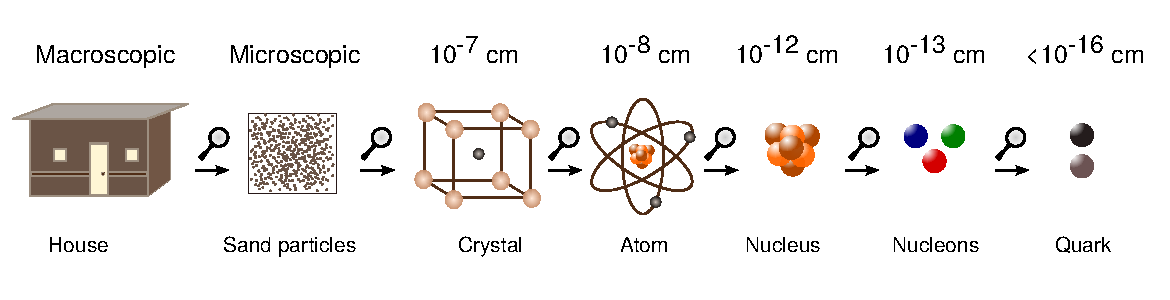
\includegraphics[width=1.0\linewidth]{Theory/Image/scale.pdf}
	  \caption{A schematic picture showing the hierarchy of building blocks
	  of the matter when one looks deeper and deeper, from right to left.
	  This figure is adopted from \cite{scienceabc}.}
  \label{fig:scale}
  \end{center}
\end{figure}

The quarks are of different types such as \textit{up} quark (\PQu), \textit{down} quark (\PQd), 
\textit{charm} quark (\PQc), \textit{strange} quark (\PQs), \textit{top} quark (t), and \textit{bottom}
quark (\PQb). The mass of each quark is different. The electric charge is 2/3 for \PQu, \PQc, \PQt 
quarks and -1/3 for \PQs, \PQb, and \PQd quarks. The electron has different partners such as 
\textit{muon} ($\mu$) and \textit{tau} ($\tau$). They differ in mass only, the electric charge 
is the same. The electron, muon, and tau are collectively called leptons. There are also 
electric-neutral partners of leptons called neutrinos such as \textit{electron-neutrino} ($\nu_e$), 
\textit{muon-neutrino} ($\nu_\mu$), and \textit{tau-neutrino} ($\nu_\tau$). The quarks are bound 
by a strong force mediated by a \textit{gluon}. The leptons interact themselves by an electromagnetic 
force mediated by a \textit{photon}. The lepton and neutrino interact by electro-weak force 
mediated by the \PW and \PZ boson. The quarks, leptons, photon, gluon, \PW/\PZ boson are 
the fundamental particles. The mass to these particles is given
by another fundamental particle called the \textit{Higgs} boson. The mass, electric charge,
and spin of all the fundamental particles are shown in Figure~\ref{fig:sm_particles}.
\begin{figure}
  \begin{center}
  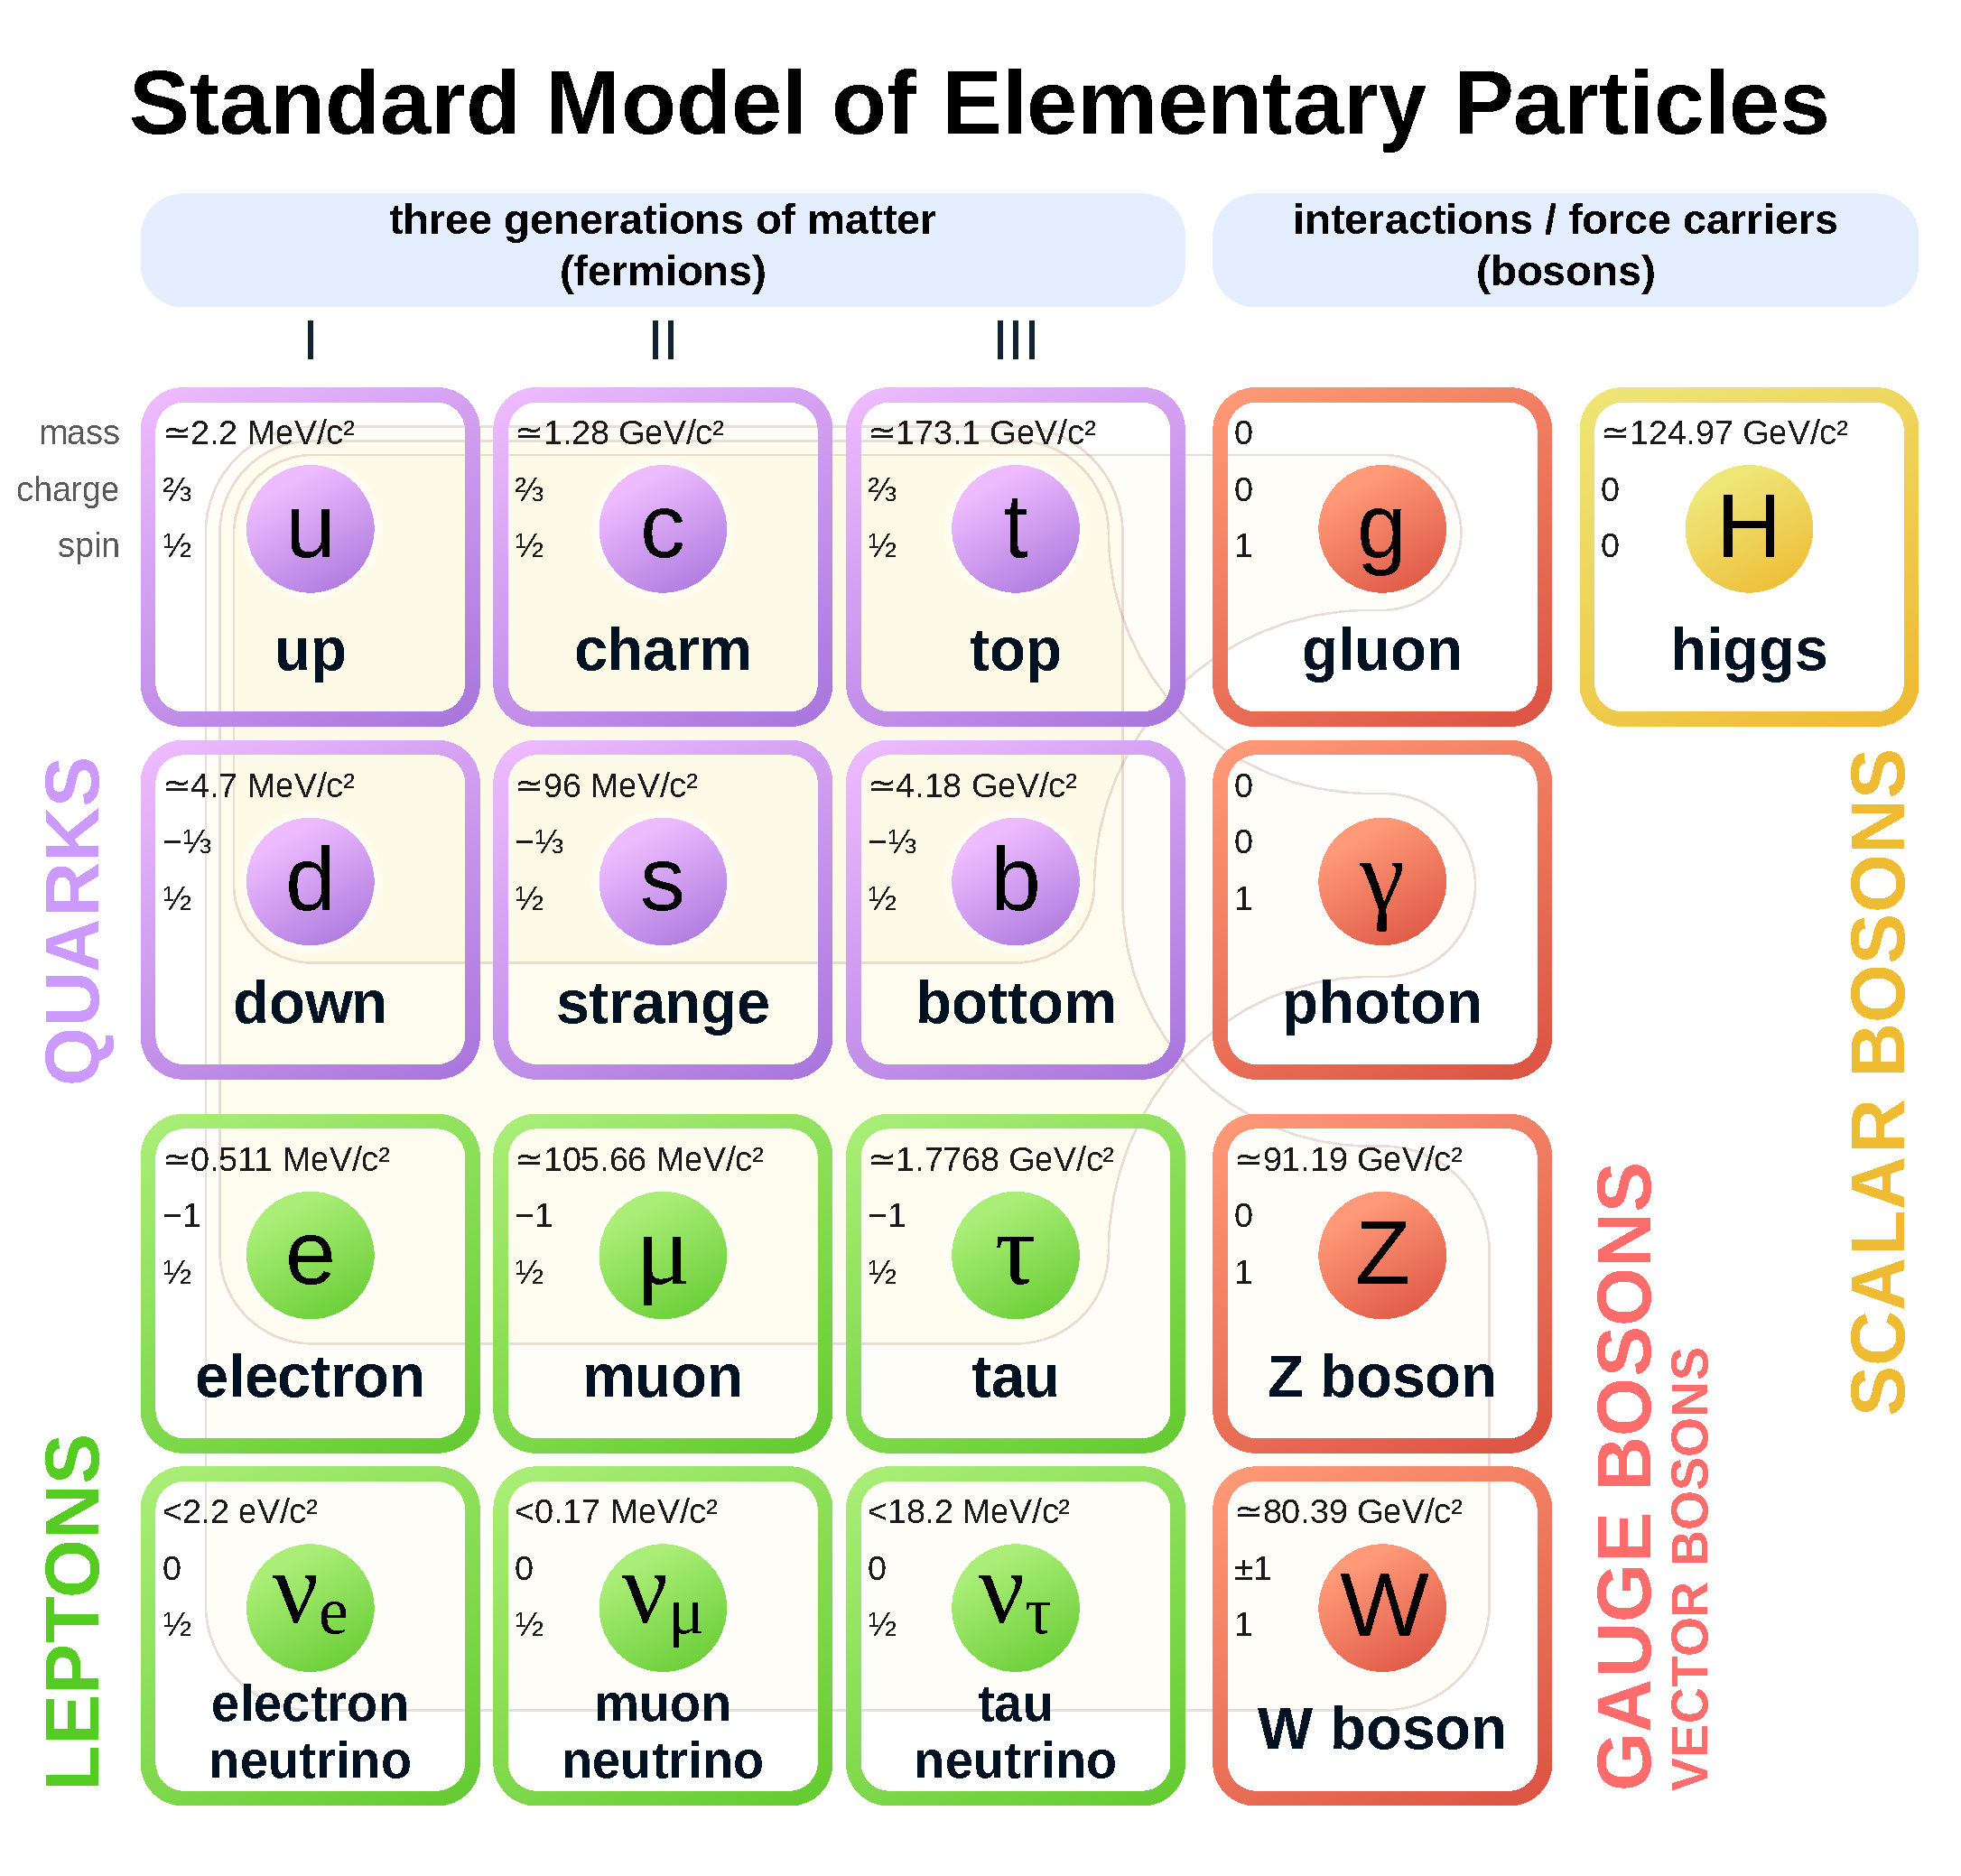
\includegraphics[width=0.80\linewidth]{Theory/Image/sm_particles.pdf}
\caption{Physical properties of the fundamental particles\cite{wikiSM}. 
	There are three generations of quarks and leptons grouped in the increasing
	order of mass. The gluon, photon, Z/W, and Higgs  bosons are force carriers.} 
  \label{fig:sm_particles}
  \end{center}
\end{figure}
All the composite particles are made of fundamental particles. All the physics
process in nature involves interactions between the fundamental particles. 
The standard model of particle physics describe all the interactions of the fundamental particles, 
as shown in Figure~\ref{fig:particle_int}. Here the photon can interact with a lepton, 
quarks, and W boson. The gluon can interact with only quarks and itself. The Higgs
boson interacts with itself, electron, muon, tau, \PW, \PZ, and all the quarks. 

The discovery of all the fundamental particles took centuries. Some of them were 
theoretically predicted many years before being experimentally observed.
The timeline of the fundamental particles are shown in Figure~\ref{fig:particle_timeline}. 
The electron was the first elementary particle to
be theorized and discovered in the late 19$^{\rm{th}}$ century. The photon, electron-neutrino,
and muon were discovered in the first 50\unit{yrs} of the 20$^{\rm{th}}$ century. All the quarks, 
except the \PQt quark, were discovered in the 60's and 70's of the 20$^{\rm{th}}$ century. The
Higgs boson is the only particle discovered in the 21$^{\rm{st}}$ century which took 48\unit{yrs}, 
it was theoretically predicted in 1964. A brief history of elementary particles 
can be found in \cite{Griffiths:111880}.
\begin{figure}
  \begin{center}
  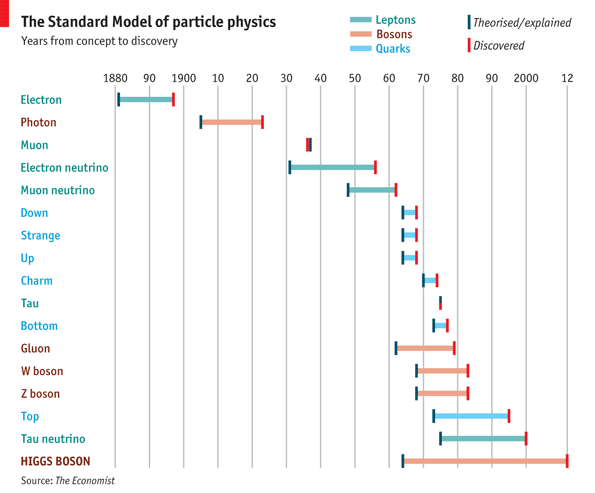
\includegraphics[width=0.75\linewidth]{Theory/Image/particle_timeline.png}
	  \caption{A timeline of the fundamental particles from their theoretical 
	prediction to the experimental observation.}
  \label{fig:particle_timeline}
  \end{center}
\end{figure}

\begin{figure}
  \begin{center}
  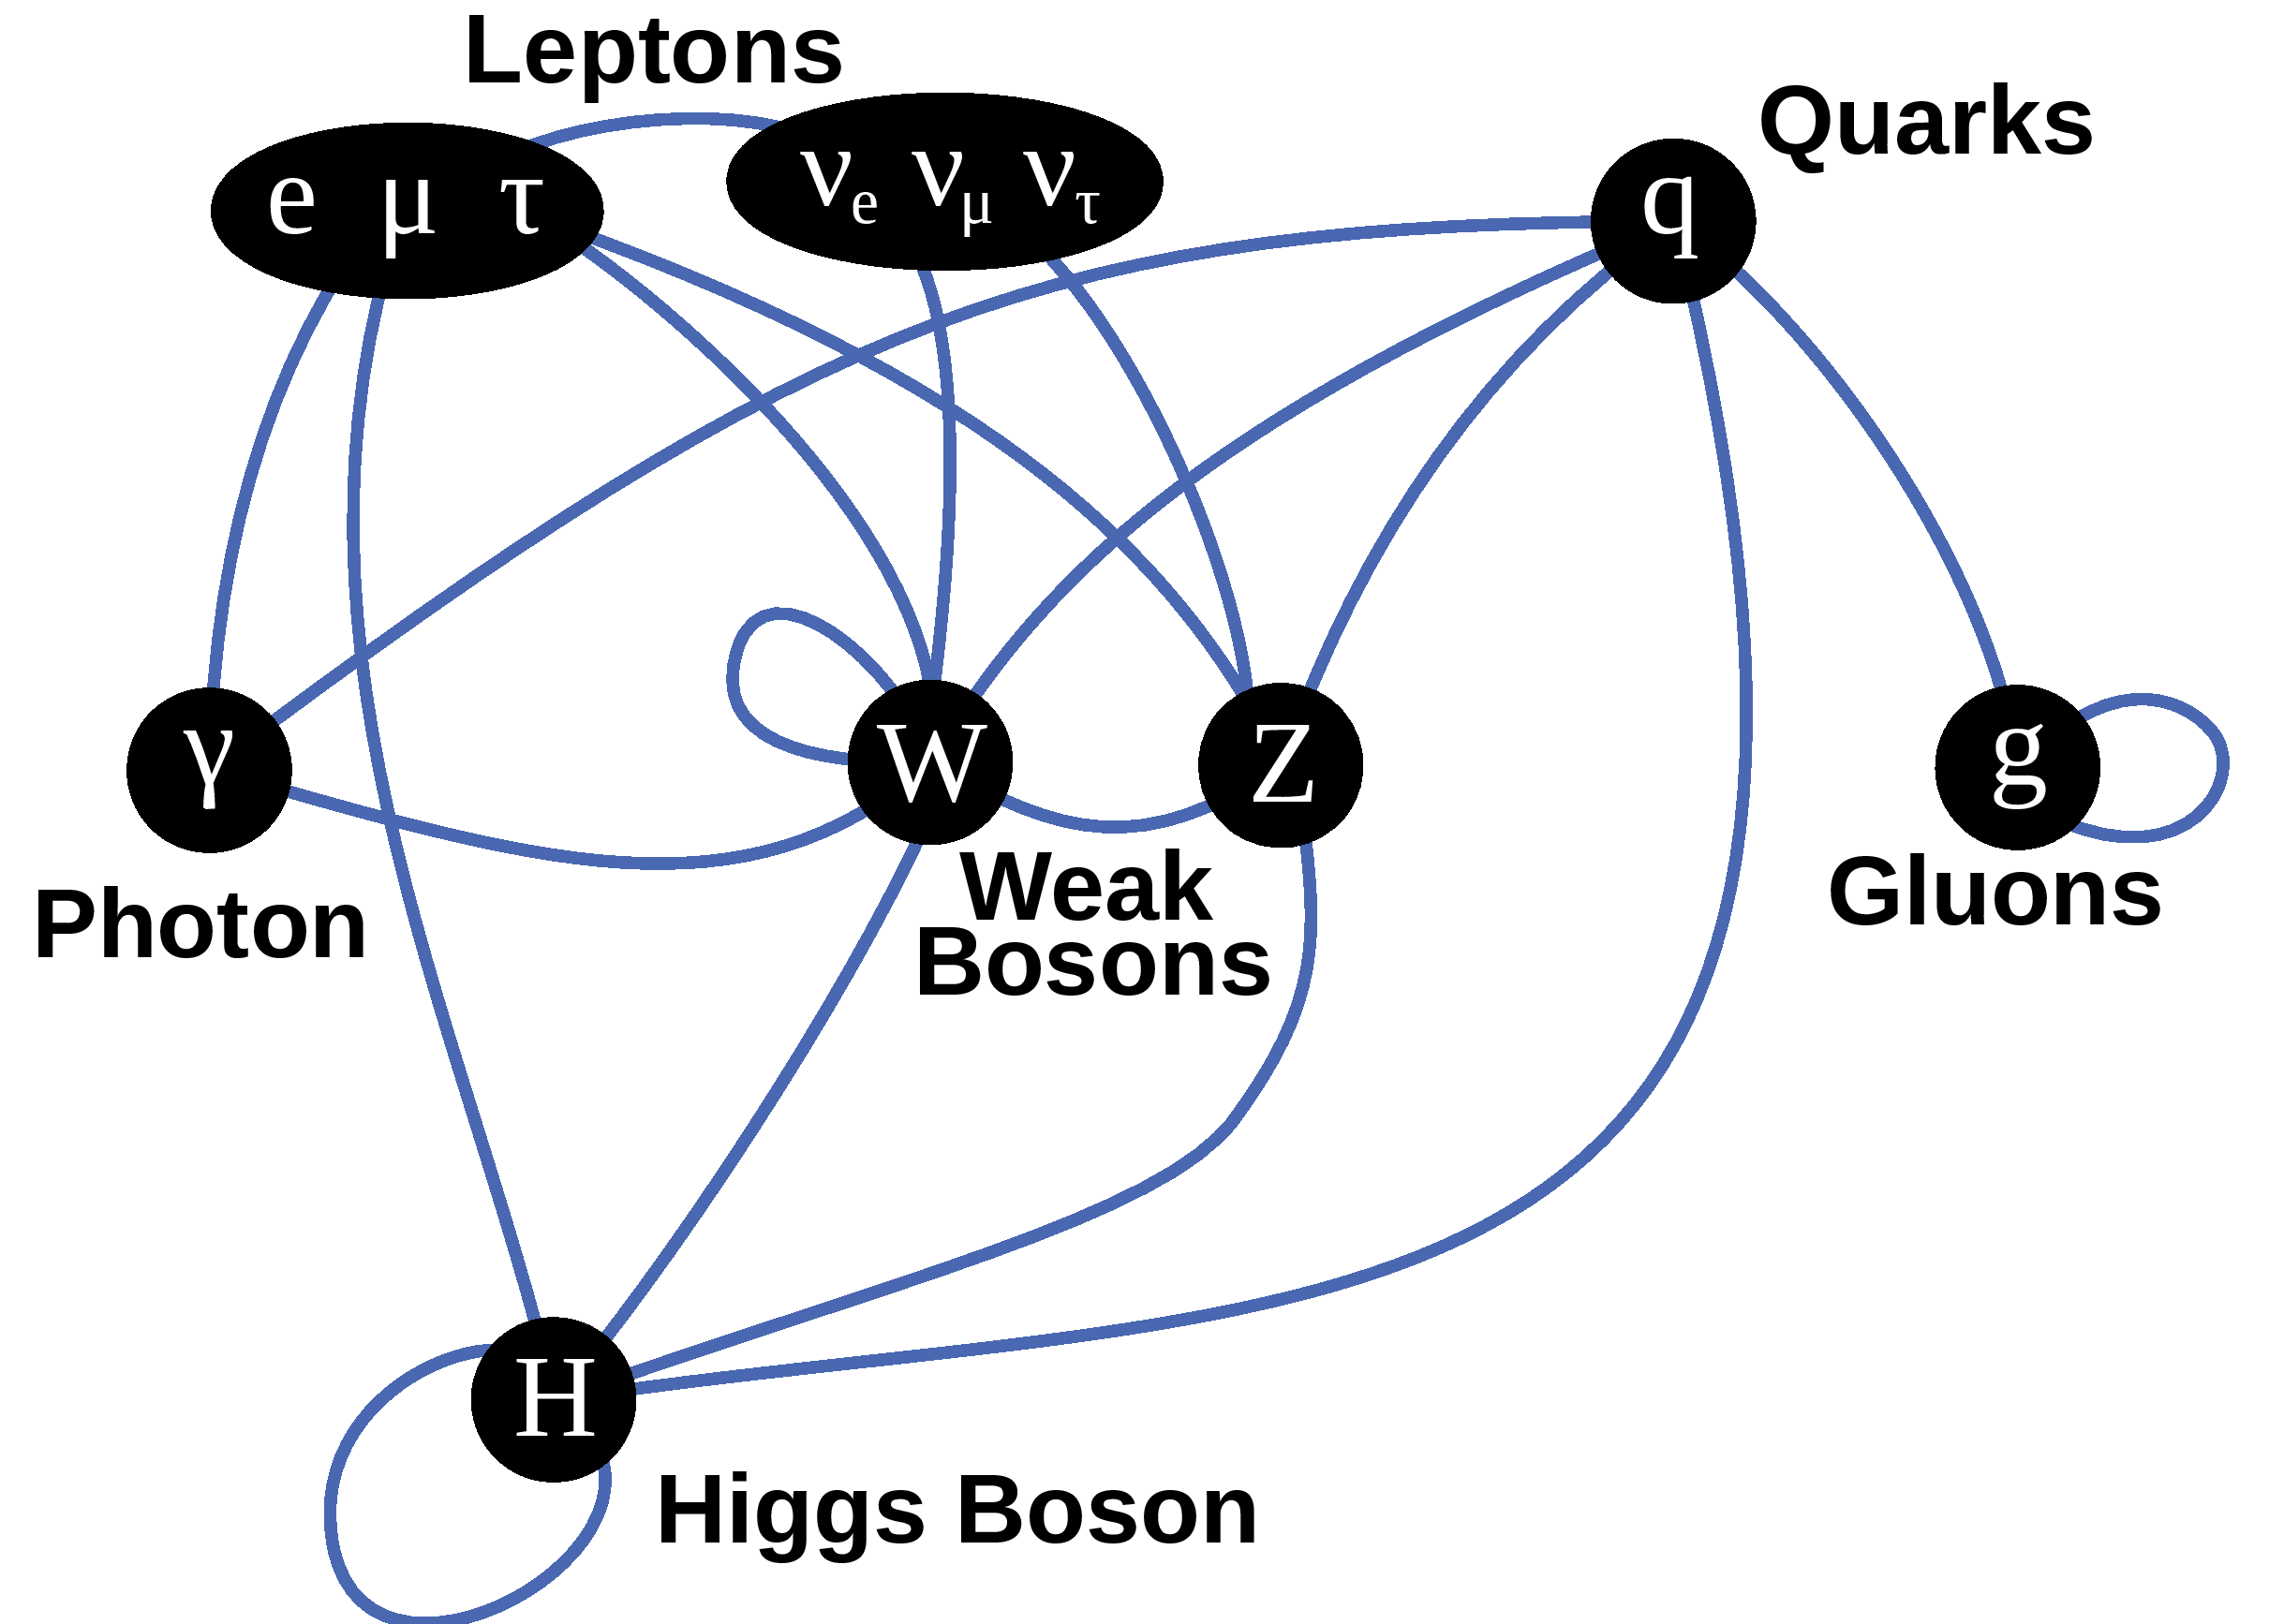
\includegraphics[width=0.50\linewidth]{Theory/Image/particle_int.png}
	\caption{A schematic diagram showing the interactions of fundamental 
	particles among themselves\cite{Isildak:2013kfa}.} 
  \label{fig:particle_int}
  \end{center}
\end{figure}

 

\section{Group and symmetry}
\label{s:smGroup}
In mathematics, a set $(G, \times)$ is called a group with respect to the 
multiplicative ($\times$) operator if the following conditions are satisfied: 
\begin{enumerate}
\item there exist an identity ($I$) element in $G$ so that $I\times g = g\times I = 
g$ where g is an element of $G$, 
\item the elements of the group follow associative 
law that is $(g_1\times g_2)\times g_3$ = $g_1\times (g_2\times g_3)$, and 
\item there exist an inverse of every element of $G$ so that $g\times g^{-1} = g^{-1}\times g = I$. 
\end{enumerate}
The group $(G, \times)$ is called an abelian group if 
the elements also follow commutative law that is $g_1\times g_2 = g_2\times g_1$. An example of a group in physics is the continuous rotation group. In general,
all the elements of a group can be generated by the parameters and generators 
of the group. For Lie groups, an element is given by $e^{i\alpha_a\tau_a}$ where
$\alpha_a$ (a = 1, 2, .., n) are the parameters and $\tau_a$ are the generators. For the theory 
of the standard model, we need the following three groups.
\begin{itemize} [leftmargin=*]
				\item \textbf{U(1)}: The unitary $1\times 1$ matrices form the U(1) 
								group. An element of the U(1) is given by $e^{i\alpha}$ where 
								$\alpha$ is the parameter. The identity element is the 
								generator of U(1).
				\item \textbf{SU(2)}: The elements of special unitary (SU) group are 
								$2\times 2$ unitary matrices. The \dq{special} implies that the
								determinant of each matrix is 1. There are in total 3 generators
								(the three Pauli matrices). All the elements of the SU(2) can be 
								constructed using these generators ($\tau_a$) and a set of 
								parameters ($\alpha_a$). An element of the SU(2) is given by 
								$e^{i\alpha_a\tau_a}$, where a = 1, 2,3. Out of three generators,
								one is diagonal. In general, the element of the SU(2) group do not 
								commute. Therefore, SU(2) is a non-Abelian group.
				\item \textbf{SU(3)}: A set of $3\times 3$ unitary matrices form the
								SU(3) group. There are 8 generators (Gell-Mann matrices) of the
								SU(3), two out of eight are diagonal. An element of the SU(3) 
								is given by $e^{i\alpha_a\lambda_a}$ where a = 1, 2, ..8, and
								$\lambda_a$ are the Gell-Mann matrices. In general, for a SU(N), 
								there are $N^2 -1$ generators, out of which $N-1$ are diagonal. 
								The SU(3) group is also non-Abelian.
\end{itemize}

A physical system is said to be invariant if it does not change under the
transformation of a group. For example, a function $f(\psi)$ is invariant 
under SU(2) if $f(\psi^\prime) = f(\psi)$ where $\psi^\prime = e^{i\alpha_a\tau_a} \psi$. There could be a function of more than one variable such as 
$f(\psi,\phi)$ where one of the variables (say $\psi$) might transform under 
SU(2) however, the other variable may not transform at all under this group. In
this case also, the function $f(\psi,\phi)$ will be invariant under SU(2). 
Therefore it is important to know about the transformation law of every variable
of a function. One can also construct a function where one variable transforms 
under one group (say SU(2)) and the other variable transforms under a different 
group (say U(1)). In this case, the function is said to be invariant under 
the combined group SU(2)$\times$ U(1). However, the generators of the individual 
group must commute for the invariance under combined group.

Noether theorem \cite{Noether:1918zz} demands that there is a conserved charge 
with every global (the parameters of the group are space-time independent) symmetry. 
For example, invariance under rotations leads to conservation of angular momentum. 
The quantum numbers for U(1) and SU(2) are denoted by $Q$ (called charge) and $T$ 
(called the weak-isospin). The third component of weak-isospin is denoted by $T_3$. In 
the context of the standard model, where electro-weak lagrangian (refer Section~\ref{s:smLag}) 
is invariant under the SU(2)$_L\times $U(1) group, an other 
quantum number called the hypercharge ($Y = 2( Q - T_3)$) is assigned to every 
particle. The $L$ in the SU(2)$_L$ implies that only left-handed fermions 
transform under the SU(2) group. The right-handed fermions are singlets, that is, 
they don't transform under this group. The various quantum numbers
associated with all the fundamental particles are shown in Table~\ref{tab:smGroup}. 
From this table, it can be seen that vector bosons 
($W^+$, $W^-$, \rm{ and } $Z$) form weak-isospin triplet, left-handed fermions form weak-isospin 
doublet, the Higgs boson is also part of the weak-isospin doublet, and the rest of 
the other particles (right-handed quarks and photon) are weak-isospin singlet.
\begin{table}
\caption{The third component of the weak-isospin, hypercharge, and charge quantum 
				numbers for leptons, quarks, and bosons.}
\label{tab:smGroup}
\begin{center}
\begin{tabular}{c c c c c c c}
\hline
\hline
				\multicolumn{1}{c}{Fermion type} &\multicolumn{3}{c}{Generation}
				& \multicolumn{1}{c}{$T_3$} 
				&\multicolumn{1}{c}{Y}& \multicolumn{1}{ c}{ Q } \\
				& 1st & 2nd  & 3rd & & & \\
\hline
\hline
				Leptons &$\begin{pmatrix} \nu_e \\ e \end{pmatrix}_L$ & $\begin{pmatrix} \nu_{\mu} \\ \mu \end{pmatrix}_L$ & $\begin{pmatrix} \nu_{\tau} \\ \tau \end{pmatrix}_L$  & $\begin{pmatrix} \frac{1}{2} \\ $-$\frac{1}{2} \end{pmatrix}$ & -1 & $\begin{pmatrix} 0 \\ $-1$ \end{pmatrix}$\\ [0.4cm]
				&$e_R$  & $\mu_R$ & $\tau_R$ & 0 & -2 & -1\\ [0.2cm]
				Quarks &$\begin{pmatrix} u \\ d \end{pmatrix}_L$ & $\begin{pmatrix} c \\ s \end{pmatrix}_L$ & $\begin{pmatrix} t \\ b \end{pmatrix}_L$  & $\begin{pmatrix} \frac{1}{2} \\ $-$\frac{1}{2} \end{pmatrix}$ & $\frac{1}{3}$ & $\begin{pmatrix} \frac{2}{3} \\ $-$\frac{1}{3} \end{pmatrix}$\\ [0.4cm]
				& $u_R$ & $c_R$ & $t_R$ & 0 &$\frac{4}{3}$ & $\frac{2}{3}$\\ [0.2cm]
				&$d_R$ & $s_R$ & $b_R$  & 0 & -$\frac{2}{3}$ & -$\frac{1}{3}$\\[0.2cm]\hline
				$W^+$ & & & & + 1 & 0 & + 1 \\[0.2cm]
				$W^-$ & & & & - 1 & 0 & - 1 \\[0.2cm]
				$Z$ & & & & 0 & 0 & 0 \\[0.2cm]
				$\gamma$ & & & & 0 & 0 & 0 \\[0.2cm]
				$H$ & & & & -$\frac{1}{2}$ & 1 & 0 \\[0.2cm]
\hline
\end{tabular}
\end{center}
\end{table}


\section{The Lagrangian density}
\label{s:smLag}
The physics of all fundamental particles is described by the Standard 
Model. The starting point of all physical theories is the 
construction of a Lagrangian density. The equations of motion for 
different fields, such as Klein-Gordon equation for scalar field, Dirac
equation for spinor field, Maxwell's equations of electromagnetism, etc, 
can be derived from a Lagrangian density using the Euler-Lagrange equation. For the
sake of convenience, we will call \dq{Lagrangian density} as \dq{Lagrangian} only.
The Lagrangian has to satisfy some basic principles.
First, it has to follow some symmetry principle, that is, it should be invariant under 
the transformation of the prescribed symmetry group. 
Second, the Lagrangian has to be \dq{renormalizable}. One 
of the criteria of renormalization demands that each interaction term in the Lagrangian
should have a coupling with mass dimension greater than or equals to zero 
(the mass dimension of fermion field, boson field, space-time derivative, and mass is 
3/2, 1, 1, 1, respectively). The advantage of Lagrangian formulation is that the Feynman 
rules can be obtained just by looking at the mathematical structure of individual terms, 
for example, the propagator is determined by the quadratic terms, and the vertex factor is 
determined by the interaction terms. The standard model (SM) is a unified theory incorporating 
electromagnetic, weak, and strong interactions. The SM Lagrangian is invariant 
under the SU(3)$_C\times$ SU(2)$_L\times$ U(1)$_Y$ group and written as
\begin{equation}
	\mathcal{L}_{\text{SM}} =  \mathcal{L}_\text{EW} + \mathcal{L}_\text{QCD} +
	\mathcal{L}_\text{H} + \mathcal{L}_\text{Yukawa}
  \label{eq:smLag}
\end{equation}
where individual terms are from electroweak, quantum chromodynamics, Higgs, and
Yukawa sectors. A detailed description of each individual term is given below.

\begin{itemize} [leftmargin=*]
\item \textbf{$\mathcal{L}_\text{EW}$}: The electro-weak (EW) Lagrangian
				follows SU(2)$_L\times$ U(1)$_Y$ symmetry and incorporates the interaction 
				between leptons (and quarks) and electro-weak gauge bosons along with the respective kinetic 
				energy terms. It is written as
				\begin{equation}
								\mathcal{L}_\text{EW} = \bar L \gamma^\mu \left(i\partial_\mu 
								- g^\prime \tfrac12 Y B_\mu - g \tfrac12 \tau_\text{a} 
								W_\mu^{\text{a}}\right)L + \bar R \gamma^\mu \left(i\partial_\mu 
								- g^\prime \tfrac12 Y B_\mu \right)R - \tfrac{1}{4} W_a^{\mu\nu} 
								W_{\mu\nu}^a - \tfrac{1}{4} B^{\mu\nu} B_{\mu\nu},
				\label{eq:LagEW}
				\end{equation}
				where $L$ ($\bar{L} = L^\dagger 
				\gamma^0$) is the doublet of left-handed leptons ($e_L, \nu_{e_L}; \mu_L, 
				\nu_{\mu_L}; \tau_L, \nu_{\tau_L}$) as shown in the first row of Table 
				\ref{tab:smGroup}, $R$ is the singlet of 
				right-handed lepton (only $e_R, \mu_R, \tau_R$) as shown in the second 
				row of Table~\ref{tab:smGroup}, the $\gamma^\mu$ are the Dirac matrices, $\tau_a$ are Pauli matrices, 
				$g^\prime$ and $g$ are coupling strength of the U(1) and SU(2) group, 
				respectively. In Equation (\ref{eq:LagEW}), we have not explicitly
shown the terms corresponding to quarks. The $B_\mu$ is the U(1) gauge field, 
				$W^a$ are the SU(2) gauge fields, $B_{\mu\nu} = 
				\partial_\mu 
				B_\nu - \partial_\nu B_\mu$ and $W_{\mu\nu}^a = \partial_\mu W_\nu^a - 
				\partial_\nu W_\mu^a + g \epsilon^{abc}W_\mu^bW_\nu^c$ are the 
				corresponding field strength tensors. Here $\epsilon^{abc}$ is totally 
antisymmetric Levi-Civita symbol. The $Y$ in Equation (\ref{eq:LagEW}) is the 
				hypercharge of the U(1) group. The summation in Equation (\ref{eq:LagEW}) 
				runs over three spaces; three generation of lepton, three generators of 
				the SU(2)(a = 1, 2, 3), and the 4 Lorentz indices ($\mu$ = 0, 1,2 ,3). 
				In Equation (\ref{eq:LagEW}), there is no coupling of $W^a$ with the 
				right-handed lepton, as they interact only with the left-handed 
				lepton. Under
				the SU(2)$_L\times$ U(1)$_Y$ group, the field $L, ~R, ~B_\mu$, and $W_\mu^a$ transform as $L^\prime = 
				e^{i\alpha_a(x)T^a + i\beta(x)Y}L, ~R^\prime = e^{i\beta(x)Y}R, 
				~B_\mu^\prime = B_\mu + \frac{1}{e}\partial_\mu\alpha(x), ~W_\mu^{\prime a}
				= W_\mu^a - \frac{1}{g}\partial_\mu\alpha_a(x) - f_{abc}\alpha_b(x) 
				W^c_\mu$, where $\alpha (x)$ and $\beta (x)$ are the local gauge parameters
				of the SU(2) and U(1) group, respectively. The Lagrangian $\mathcal{L}_\text{EW}$ is 
				invariant under these transformations.

\item \textbf{$\mathcal{L}_\text{QCD}$}: The Lagrangian for the quantum
chromodynamics involves the interactions of quarks and gluons and 
respects SU(3) symmetry. Unlike the lepton, the quarks have an additional 
color quantum number called \dq{color}. The Lagrangian is given as
\begin{equation}
\mathcal{L}_\text{QCD} = \bar Q_{i} \left( i\gamma^\mu(
\partial_\mu\delta_{ij} - i g_s G_\mu^a T^a_{ij})\right) Q_j
- \frac{1}{4} G^a_{\mu\nu} G^{\mu\nu}_a,
\label{eq:LagQCD}
\end{equation}
where the $i$ in $Q_i$ is the color index for $R$, $G$, and $B$. The $Q$ is
the Dirac spinor for each quark, $g_s$ is the strength
of strong coupling, $T^a$ are 8 (a = 1, 2, .., 8) generators of the SU(3)
also called Gell-Mann matrices, $G^a$ are the gauge fields of the strong 
interaction, $G_{\mu\nu}^a = \partial_\mu G_\nu^a - \partial_\nu G_\mu^a + g 
f^{abc}G_\mu^bG_\nu^c$ are the gluon field strength tensors, and $f^{abc}$ 
are the structure constants of SU(3). There are five summations involved
in Equation (\ref{eq:LagQCD}): quark family (Q = u, d, c, s, t, b), 
chirality of quarks, color (i = 1, 2, 3), a = 1, 2, .., 8, and
Lorentz ($\mu$ = 0, 1, 3, 4). Under the SU(3), the two fields transform as 
$Q^\prime = e^{i\alpha_a(x)T^a }Q, ~G_\mu^{\prime a} = G_\mu^a - 
\frac{1}{g}\partial_\mu\alpha_a(x) - f_{abc}\alpha_b(x) G^c_\mu$. The 
Lagrangian $\mathcal{L}_\text{QCD}$ is invariant under these transformations.

\item \textbf{$\mathcal{L}_\text{H}$}: The Higgs sector of the SM incorporates
				interaction of Higgs fields with gauge bosons of SU(2) and U(1) groups
				as well as a potential energy term for Higgs. The Higgs field is part 
				of a complex scalar doublet of the SU(2) group. The Lagrangian density is 
				given as
				\begin{equation}
				\mathcal{L}_\text{H} = \left|\left(\partial_\mu + \frac{i}{2} \left( 
								g^\prime Y B_\mu + g \tau_a W_\mu^a \right)\right)\varphi
								\right|^2 - V(\varphi), 
				\label{eq:LagHiggs}
				\end{equation}
				where the Higgs doublet is defined as
				\begin{equation}
				\varphi = \frac{1}{\sqrt 2} \left(\begin{array}{c}\varphi^+ \\ 
				\varphi^0\end{array}\right),
				\end{equation}
				with $\varphi^+$ and $\varphi^0$ having electrical charge +1 and 0, 
respectively. 
				The hypercharge of both fields is 1. The potential term for the Higgs 
				field $V(\varphi)$ is given in Section~\ref{s:smMass}. Under the SU(2)
				group, the Higgs doublet transforms as $\varphi^\prime = e^{i\alpha_a(x)
				\tau^a}\varphi$. The transformation law for the other two fields of 
				Equation (\ref{eq:LagHiggs}) is described in $\mathcal{L}_\text{EW}$. 
				The mass to the vector bosons is generated in $\mathcal{L}_\text{H}$ as
				discussed in Section~\ref{s:smMass}.

\item \textbf{$\mathcal{L}_\text{Yukawa}$}: The interactions of fermions (quarks and leptons) with 
Higgs boson are described by the Yukawa Lagrangian. It is written as 
\begin{equation}
\mathcal{L}_\text{Yukawa} =  G_l\bar L \varphi R + G_d \bar{q_L} \varphi d_R +G_u \bar{q_L} \varphi_c u_R + h.c.,
\end{equation}
where $G_l$ is the coupling of Higgs to lepton, $G_d$ ($G_u$) is the coupling
of Higgs to up (down) quark, and $\varphi_c = -i\tau_2\varphi^{\text{*}}$. 
\end{itemize}
    

\section{Mass of particles}
\label{s:smMass}

The Lagrangian, given in Equation (\ref{eq:smLag}), is complete in the sense that it 
is invariant under the SU(3)$_C\times $SU(2)$_L\times$ U(1)$_Y$ group and it is 
renormalizable. However, except for the Higgs boson, the mass terms for
other particles, such as the fermion mass term 
$m\bar\psi \psi$, 
are not included in Equation (\ref{eq:smLag}). The 
mass term for the Higgs boson is included in the potential 
\begin{equation}
V(\varphi) = \left(\partial_\mu\varphi\right)^\dagger \left(\partial^\mu
\varphi\right) - \mu^2\varphi^\dagger\varphi - \lambda\left(
\varphi^\dagger\varphi\right)^2,
\label{eq:potPhi}
\end{equation}
where, 
\begin{equation}
\varphi = \frac{1}{\sqrt 2} \left(\begin{array}{c}\varphi_1 (x) + 
i\varphi_2 (x) \\ \varphi_3 (x) + i\varphi_4 (x) \end{array}\right),
\label{eq:higgsPhi}
\end{equation}

After substituting $\varphi$ from Equation (\ref{eq:higgsPhi}) to the potential of
Equation (\ref{eq:potPhi}), it can be easily seen that all the four Higgs fields 
have a mass term of type $\mu^2\varphi_i^2$ where i = 1,2, 3, 4, where $\mu^2 < 0$. This
lead to spontaneous symmetry breaking as discussed in the next section.
Note that $\mu$ is not the physical mass of the Higgs particle. 
The physical masses of 
all particles are generated by the spontaneously breaking of symmetry 
\cite{PhysRev.127.965} and the Higgs mechanism 
\cite{PhysRevLett.13.321,HIGGS1964132,Isildak:2013kfa,PhysRevLett.13.508,PhysRevLett.13.585,PhysRev.145.1156,PhysRev.155.1554} as discussed below. 
\begin{itemize}[leftmargin=*]
\item \textbf{Spontaneous symmetry breaking (SSB) and Higgs mechanism}: 
The minima of the potential 
$V(\varphi)$ correspond to $\varphi_1^2 + \varphi_2^2 + 
\varphi_3^2 + \varphi_4^2 = v^2$, where $v = \sqrt{-\mu^2/\lambda}$ 
is the vacuum expectation value (vev), $\mu^2 < 0$, and $\lambda > 
0$. Next we  
 expand the potential about the minima.  
The minima can be chosen at 
$\varphi_1 = \varphi_2 = \varphi_4 = 0, \varphi_3 = v$, and the
potential in the Lagrangian $\mathcal{L}_H$ is expanded about this
minimum. That is, the field given by Equation (\ref{eq:higgsPhi})
is re-written as 
\begin{equation}
\varphi = \frac{1}{\sqrt 2} \left(\begin{array}{c} \varphi_1(x)+i\varphi_2(x)
\\ v + h(x) + i\varphi_4(x) \end{array}\right),
\label{eq:higgsPhi2}
\end{equation}
It turns out that the fields $\varphi_1$, $\varphi_2$ and $\varphi_4$ are
not physical and get eliminated from the physical particle spectrum. We 
see this by reparametrizing this equation as,
\begin{equation}
\varphi = \frac{e^{i\tau_a\theta^a(x)/v}}{\sqrt{2}}
\left(\begin{array}{c} 0
\\ v+h(x) \end{array}\right),
\label{eq:higgsPhi3}
\end{equation}
where $\theta^a$ are three new fields. We can now eliminate these fields 
by a gauge transformation. The Higgs multiplet can now be expressed as
\begin{equation}
\varphi = \frac{1}{\sqrt{2}}
\left(\begin{array}{c} 0
\\ v+h(x) \end{array}\right),
\label{eq:higgsPhi4}
\end{equation}
The resulting gauge choice is called the unitary gauge. In this gauge, only the physical Higgs field appears in the Lagrangian and
all the other scalar fields get eliminated. After substituting $\varphi$ from 
Equation (\ref{eq:higgsPhi4}) in $\mathcal{L}_H$, mass terms appear for gauge 
bosons $B_\mu$, $W_1$, $W_2$, and $W_3$. Furthermore the Higgs
field acquires physical mass. The other three scalar degrees of freedom now
act as the longitudinal modes of the massive gauge bosons. 

The $\mathcal{L}_H$ now contains only gauge fields $B_\mu, W_\mu^a$ and
the $h(x)$ with respective mass terms. We next identify the physical
gauge boson particle spectrum. We note that the vacuum preserves
the electromagnetic 
 $U(1)_{em}$ symmetry since 
 $\varphi_3$ has zero electric charge ($T^3 = -1/2$, 
$Y = 2$, hence $Q = 0$) hence does not transform under the 
$U(1)_{em}$ group. The gauge
bosons  are expressed in a new basis as 
$W^\pm = (W^1 \mp iW^2)/ \sqrt{2}, ~A_\mu = \cos\theta_W B_\mu 
+ \sin\theta_W W^3_\mu,
~Z_\mu = -\sin\theta_W B_\mu + \cos\theta_W W^3_\mu$. After writing
$\mathcal{L}_H$ in terms of $A_\mu, ~Z_\mu, ~W^\pm$, one can see that
the $A_\mu$ becomes massless and $W^\pm$, $Z_\mu$ remain
massive with masses $ \frac{1}{2}vg, ~\frac{1}{2}v\sqrt{g^2 + 
g^{\prime}}$, respectively. The mass of leptons (electron, muon, 
and tau) and quarks are generated using Equation (\ref{eq:higgsPhi3})
in $\mathcal{L}_{\rm{Yukawa}}$. The neutrino in the SM remains massless. 
\end{itemize}

Notice that before the symmetry breaking, there were 4 massless (gauge bosons) and 4 
scalar particles. The polarization degree of freedom ($P_{\text{dof}}$) 
for each Higgs is 1 and for each massless gauge boson is 2. 
Therefore, total $P_{\text{dof}}$ before the SSB is $4\times1 + 4\times 
2 = 12$. After the SSB, the massive gauge bosons get an additional $P_{\text{dof}}$
from the three scalar boson. Therefore, the total number of $P_{\text{dof}}$ after the SSB 
is also 12 ($1\times 1 + 3\times 0 + 1\times 2 + 3\times 3$). 

The masses of all the fundamental particles are shown in 
Table~\ref{tab:massSM} in terms of free parameters. However, the value of these 
parameters is determined from experiment.
Until now, the Lagrangian $\mathcal{L}_{\rm{SM}}$ contains 14 free parameters which 
are 3 couplings of gauge groups ($g, ~g^\prime, ~g_s$), 2 from Higgs field 
($v, ~\lambda$), 3 couplings ($G_l$) of Higgs-lepton interactions, and 6 couplings
($G_q$) of Higgs-quark interactions. There are 5 additional free parameters in the
SM which are 3 CKM mixing angles ($\theta_{12}, ~\theta_{23}, ~\theta_{13}$) 
\cite{PhysRevLett.10.531}, 1 CKM CP violation phase \cite{10.1143/PTP.49.652}, 
and 1 QCD vacuum angle ($\theta_{\rm{QCD}}$). Therefore, there are 19 free parameters 
in the SM.

\begin{table} 
\caption{The mass of all fundamental particles in terms of the free parameters of
				the standard model with the corresponding observed values.} 
\label{tab:massSM} 
\begin{centering} 
\begin{tabular}{ccc} 
\hline 
\hline 
Particles & Theoretical mass & Experimental mass \\ 
\hline 
\hline
\noalign{\vskip 0.1cm}
				H & $v\sqrt{2\lambda}$ & 125.1 \GeV \\ \noalign{\vskip 0.1cm}
				$W^\pm $ & $\frac{1}{2}vg$ & 80.4 \GeV \\ \noalign{\vskip 0.1cm}
				Z & $\frac{1}{2}v\sqrt{g^2 + g^{\prime}}$ & 91.2 \GeV \\ \noalign{\vskip 0.1cm}
				photon & 0 & 0\\ \noalign{\vskip 0.1cm}
				gluon & 0 & 0\\ \noalign{\vskip 0.1cm}
				$e, ~\mu, ~\tau$ & $\frac{G_lv}{\sqrt{2}}$ & shown in 
				Figure~\ref{fig:sm_particles}\\ \noalign{\vskip 0.1cm}
				neutrino & 0 & shown in Figure~\ref{fig:sm_particles}\\ \noalign{\vskip 0.1cm}
				Quarks & $\frac{G_qv}{\sqrt{2}}$  & shown in Figure~\ref{fig:sm_particles}\\
				\noalign{\vskip 0.1cm}
\hline 
\end{tabular} 
\par\end{centering} 
\end{table}

\section{Success and failure of the SM}
\label{s:meritSM}
The standard model is a mathematically complete and experimentally tested theory.
However, it does not provide explanations to all of the observed phenomena in
nature. A brief description of successes and failures of the SM is given below.
\begin{itemize}[leftmargin=*]
				\item \textbf{Success}: The SM describes the interaction among the 
								fundamental particles with excellent accuracy. The electro-weak
								gauge bosons ($W^\pm, ~Z$), gluon, top and charm quarks were
								predicted by the SM before being observed experimentally. The
								Higgs boson was predicted in 1964 and experimentally observed in
								2012 \cite{Aad:2015zhl}. Value to all the free parameters of the 
								SM has been experimentally assigned. The predictions from the SM 
								agree very well with the experimental observations.

\item \textbf{Failure}:
There are many shortcomings of the SM. A few of them are mentioned below:  
\begin{itemize}[leftmargin=*]
\item The $\mathcal{L}_{SM}$ includes 
three generations of leptons. However, only the first generation ($e, \nu_e$) is 
enough to form the nucleus and hence the visible content of the universe. The SM
does not provide any explanation for the existence of the second and the third
generations or why there should not be more than three?
\item The neutrinos in the SM are massless. However, it is observed by 
the SNO experiment that neutrinos do have a small mass. 
\item Third, why the Lagrangian $\mathcal{L}_{\rm{SM}}$ does not 
include gravity?
\item The SM does not explain the origin of dark matter \cite{Ade:2013zuv,
Ade:2013sjv} and dark energy which account for about 96\% of the universe. 
\item Why there are so many (19) free parameters in the SM? 
\item Why there is more matter than antimatter, etc? 
\end{itemize}
\end{itemize}
To explain the shortcomings of the SM, many beyond the standard model (BSM) 
theories have been proposed such as grand unified theories, supersymmetry 
\cite{Martin:1997ns}, etc. One of the extensions of the SM is described in the 
next chapter.


\chapter{The Two Higgs Doublet Model}
\label{c:sec2HDM}

\section{Introduction}
\label{s:secIntro2HDM}
As described in Section~\ref{s:meritSM}, although the predictions of the SM 
match well with the experimental observation, the SM has no explanation
to many other observed phenomena. To be able to explain such phenomena, 
many extensions of the SM have been proposed. One of the simplest
extensions is the two Higgs doublet model (2HDM) where an extra Higgs doublet is
added to Equation~(\ref{eq:smLag}). In Lagrangian of the SM, there is only one Higgs SU(2) 
doublet comprising four Higgs fields. After the spontaneous symmetry breaking, 
only one Higgs ($h$) remains in the model as the other three Higgses are eaten 
away by the three gauge bosons ($W^\pm, ~Z$). In the 2HDM, there are two SU(2) 
Higgs doublets comprising eight Higgs fields. Three of them are again 
eaten away by the gauge bosons and the five Higgses ($h, H, A, H^\pm$) remains 
in the model. Further, the 2HDM is divided into four types (I, II, X, Y) based 
on the coupling of quarks and leptons with the two Higgs doublets. The type II
of the 2HDM corresponds to the MSSM (minimal supersymmetric extension of the 
standard model).
% in the limit where the mass of each particle is decoupled on a very large scale.

\section{The Higgs sector}
The Higgs potential term for the 2HDM is constructed in such a way so that it is 
invariant under Z$_2$ symmetry, where the Higgs doublets transform as 
$\Phi_1 \rightarrow \Phi_1, ~ \Phi_2 \rightarrow \text{-} \Phi_2$. The Z$_2$ symmetry
is imposed to avoid the flavor changing neutral currents (FCNC). The CP-conserving 
potential is given by \cite{PhysRevD.80.015017}
\begin{align}
V^\text{2HDM}
&= m_1^2\Phi_1^\dag\Phi_1+m_2^2\Phi_2^\dag\Phi_2
-m_3^2\left(\Phi_1^\dag\Phi_2+\Phi_2^\dag\Phi_1\right)
+\frac{\lambda_1}2(\Phi_1^\dag\Phi_1)^2
+\frac{\lambda_2}2(\Phi_2^\dag\Phi_2)^2\nonumber \\
&\qquad+\lambda_3(\Phi_1^\dag\Phi_1)(\Phi_2^\dag\Phi_2)
+\lambda_4(\Phi_1^\dag\Phi_2)(\Phi_2^\dag\Phi_1)
+\frac{\lambda_5}2\left[(\Phi_1^\dag\Phi_2)^2
+(\Phi_2^\dag\Phi_1)^2\right], 
\label{eq:pot2HDM}
\end{align}
where $m_i$ and $\lambda_i$ are scalar potential parameters taken to be real. 
The parameters are chosen such that the potential admits spontaneous symmetry breaking. Let $v_i$ be
the vacuum expectation value (vev) of the Higgs field $\Phi_i$. We expand
the Higgs field around its vev~\cite{PhysRevD.80.015017}, such that,

\begin{align}
\Phi_i=\begin{pmatrix}\omega_i^+\\\frac1{\sqrt2}(v_i+h_i-i\,z_i)
\end{pmatrix}.
\label{eq:higgs2HDM}
\end{align}
After substituting new fields from Equation (\ref{eq:higgs2HDM}) into (\ref{eq:pot2HDM}), 
one can see that there are off-diagonal terms for 
$\omega_i^+, ~ h_i, ~z_i$ fields. To remove these off-diagonal terms from the 
potential, these fields are reparametrized in terms of new fields $\omega^\pm, 
~H^+, ~z, ~A, ~h,$ and $H$ by using the following transformations \cite{PhysRevD.80.015017}
\begin{align}
\begin{pmatrix}h_1\\h_2\end{pmatrix}=\text{R}(\alpha)
\begin{pmatrix}H\\h\end{pmatrix},\quad
\begin{pmatrix}z_1\\z_2\end{pmatrix}=\text{R}(\beta)
\begin{pmatrix}z\\A\end{pmatrix},\quad
\begin{pmatrix}\omega_1^+\\\omega_2^+\end{pmatrix}=\text{R}(\beta)
\begin{pmatrix}\omega^+\\H^+\end{pmatrix},
\end{align}
where $R(\alpha), ~R(\beta)$ are the rotation matrices given by 
\cite{PhysRevD.80.015017}
\begin{align}
\text{R}(\theta)=\begin{pmatrix}\cos\theta&-\sin\theta\\
\sin\theta&\cos\theta\end{pmatrix}.
\end{align}
After the Higgs mechanism, the three Higgses are eliminated from the potential 
terms. They are eaten away by the three gauge bosons ($W^\pm, ~Z$). The free 
parameters in the potential are masses of the remaining five Higgses, $m_3^2$, 
$v$, $\tan\beta$, and $\cos(\beta -\alpha)$, where $v = \sqrt{v_1^2 + v_2^2}$ and 
$\tan\beta = v_1/v_2$. The scalar parameters in the potential and the physical parameters are 
listed in Table~\ref{tab:param2HDM}. 
%At tree level, only two physical parameters ($\tan\beta, ~m_A$) are independent, 
%the rest can be expressed in terms of these two.
\begin{table}
\begin{centering}
\caption{The scalar potential and physical parameters of the Higgs sector of the 2HDM.}
\label{tab:param2HDM}
\begin{tabular}{cc}
	\hline \noalign{\vskip 0.2cm}
	Scalar potential parameters & $m_1, ~m_2, ~m_3, ~\lambda_1, ~\lambda_2, ~\lambda_3,
	~\lambda_4, ~\lambda_5$\\ \noalign{\vskip 0.2cm}
	Physical parameters & $m_h^2, ~m_H^2, ~m_{H^\pm}^2 ~m_A^2, ~m_3^2, ~v, 
	~\tan\beta, ~\cos(\beta-\alpha)$ \\ \noalign{\vskip 0.2cm}
	\hline
	\end{tabular}
	\par\end{centering}
\end{table}

\section{The Yukawa sector}
The Yukawa sector of the 2HDM is considerably more complicated in comparison to that
of a single Higgs doublet. The general Lagrangian free from FCNC for the Yukawa sector is 
given as
%\begin{align}
%{\mathcal L}_\text{yukawa}^\text{2HDM} =
%&-{\overline Q}_LY_u\widetilde{\Phi}_uu_R^{}
%-{\overline Q}_LY_d\Phi_dd_R^{}
%-{\overline L}_LY_\ell\Phi_\ell \ell_R^{}+\text{H.c.},
%\label{eq:lagYu2HDM}
%\end{align}
\begin{equation}
\mathcal{L}_\text{Yukawa}^\text{2HDM} =  G^l\bar L \varphi_i R + G^d \bar{q_L} \varphi_i d_R +G^u \bar{q_L} \varphi_i^c u_R + h.c.,
\label{eq:lagYu2HDM}
\end{equation}
where $i$ can be 1 or 2. The interactions of the two Higgs doublets are different for different 
flavors of the fermions. Based on the different types of interaction, the 
2HDM is divided into four types as shown in Table~\ref{tab:type2HDM}. For example,
in Type II, the up-type quarks interact with the second Higgs doublet ($\varphi_2$), down 
type-quarks and leptons interact with the first Higgs doublet ($\varphi_1$).
\begin{table} 
\begin{centering} 
\caption{The different types of 2HDM. The quarks and leptons interact either
	with the first or the second Higgs doublet in different types.}
\label{tab:type2HDM} 
\begin{tabular}{ccccc} 
\hline 
\hline 
Coupling of &\textbf{Type-I} &\textbf{Type-II} &\textbf{Type-X} &\textbf{Type-Y}
\\ 
\hline 
\hline
\noalign{\vskip 0.1cm}
up-type quarks 	& $\Phi_2$  & $\Phi_2$ & $\Phi_2$ & $\Phi_1$ \\ 
\noalign{\vskip 0.1cm}                                                     
down-type quarks 	& $\Phi_2$  & $\Phi_1$ & $\Phi_2$ & $\Phi_2$ \\ 
\noalign{\vskip 0.1cm}                                                     
leptons 		& $\Phi_2$  & $\Phi_1$ & $\Phi_1$ & $\Phi_2$ \\ 
\noalign{\vskip 0.1cm}
\hline 
\end{tabular} 
\par\end{centering} 
\end{table}

The general form of the Lagrangian, as given by Equation (\ref{eq:lagYu2HDM}),
for all types of the 2HDM can be written as \cite{PhysRevD.80.015017}
\begin{align}
{\mathcal L}_\text{yukawa}^\text{2HDM} =
&-\sum_{f=u,d,\ell} \left( \frac{m_f}{v}G_h^f{\overline
f}fh+\frac{m_f}{v}G_H^f{\overline
f}fH-i\frac{m_f}{v}G_A^f{\overline f}\gamma_5fA\right)\nonumber\\
&-\left\{\frac{\sqrt2V_{ud}}{v}\overline{u}
\left(m_uG_A^u\text{P}_L+m_dG_A^d\text{P}_R\right)d\,H^+
+\frac{\sqrt2m_\ell G_A^\ell}{v}\overline{\nu_L^{}}\ell_R^{}H^+
+\text{H.c.}\right\},\label{Eq:Yukawa}
\end{align}
where $f$ is the fermion, $G^f_h$ is the coupling of fermion $f$ with the Higgs
boson $h$, and $P_{L/R}$ are projection operators. The value of $G^f$ is 
different for different types of the 2HDM as shown in Table~\ref{tab:coupling2HDM}. 
Only couplings with the Higgs $A$ is shown in this table
as only that is needed for the study of branching ratios of the charged Higgs boson.
Couplings of fermions with all the Higgses are given in \cite{PhysRevD.80.015017}
. The branching ratio of \PQt quark decays and the charged Higgs decays have been 
given in the next sections.
\begin{table} 
\begin{centering} 
\caption{The coupling of quarks and leptons with Higgs $A$ for all types of 2HDM.}
\begin{tabular}{ccccc} 
\hline 
\hline 
Coupling & Type-I & Type-II & Type-X & Type-Y \\ 
\hline 
\hline
\noalign{\vskip 0.1cm}
$G^u_A$ & $\cot\beta$  & $\cot\beta$ & $\cot\beta$ & $\cot\beta$ \\ 
\noalign{\vskip 0.1cm}
$G^d_A$ & $-\cot\beta$  & $\tan\beta$ & $-\cot\beta$ & $\tan\beta$ \\ 
\noalign{\vskip 0.1cm}
$G^l_A$ & $-\cot\beta$  & $\tan\beta$ & $\tan\beta$ & $-\cot\beta$ \\ 
\noalign{\vskip 0.1cm}
\hline 
\end{tabular} 
\par\end{centering} 
\label{tab:coupling2HDM} 
\end{table}


%\begin{figure}
%\begin{center}
%\begin{minipage}{0.24\hsize}
%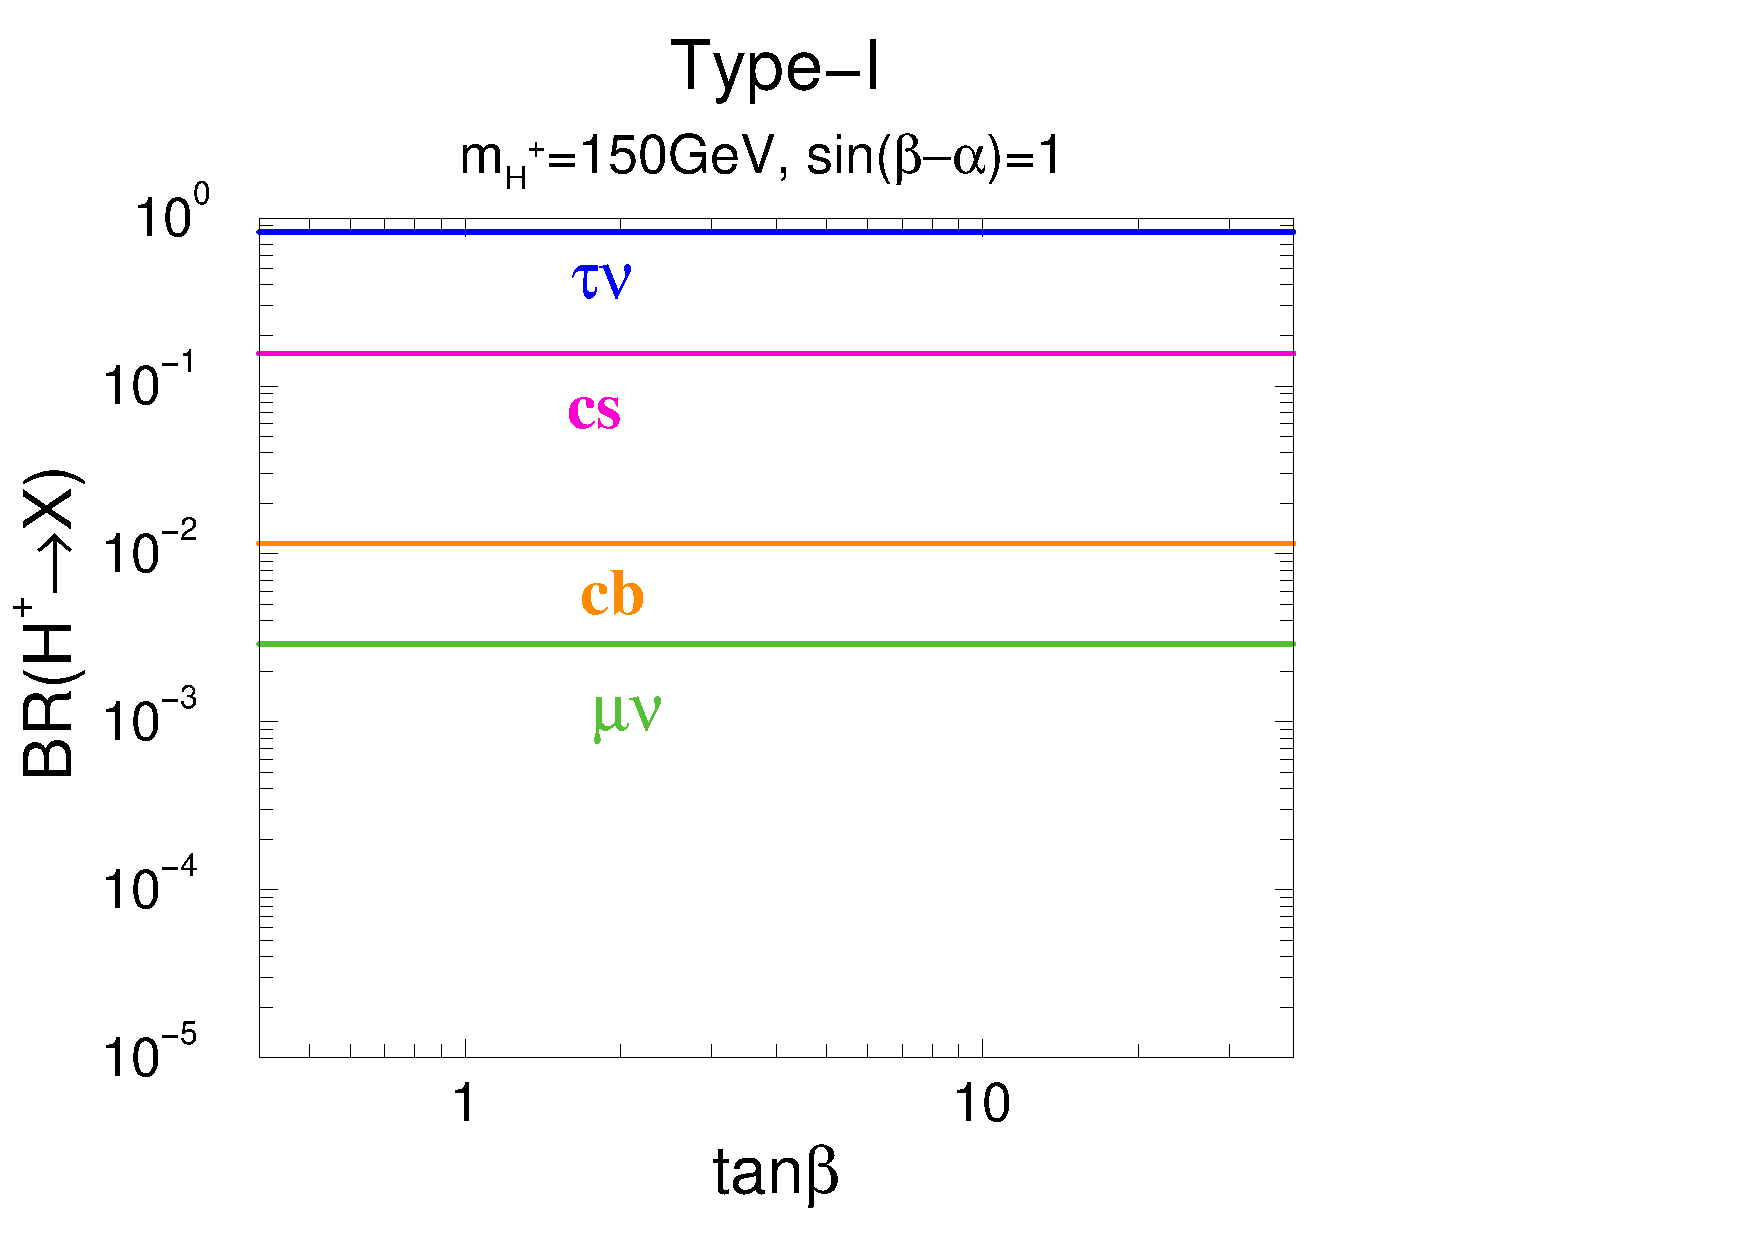
\includegraphics[width=1.7\linewidth]{Theory/Image/BR_ch_1.pdf}
%\end{minipage}
%\begin{minipage}{0.24\hsize}
%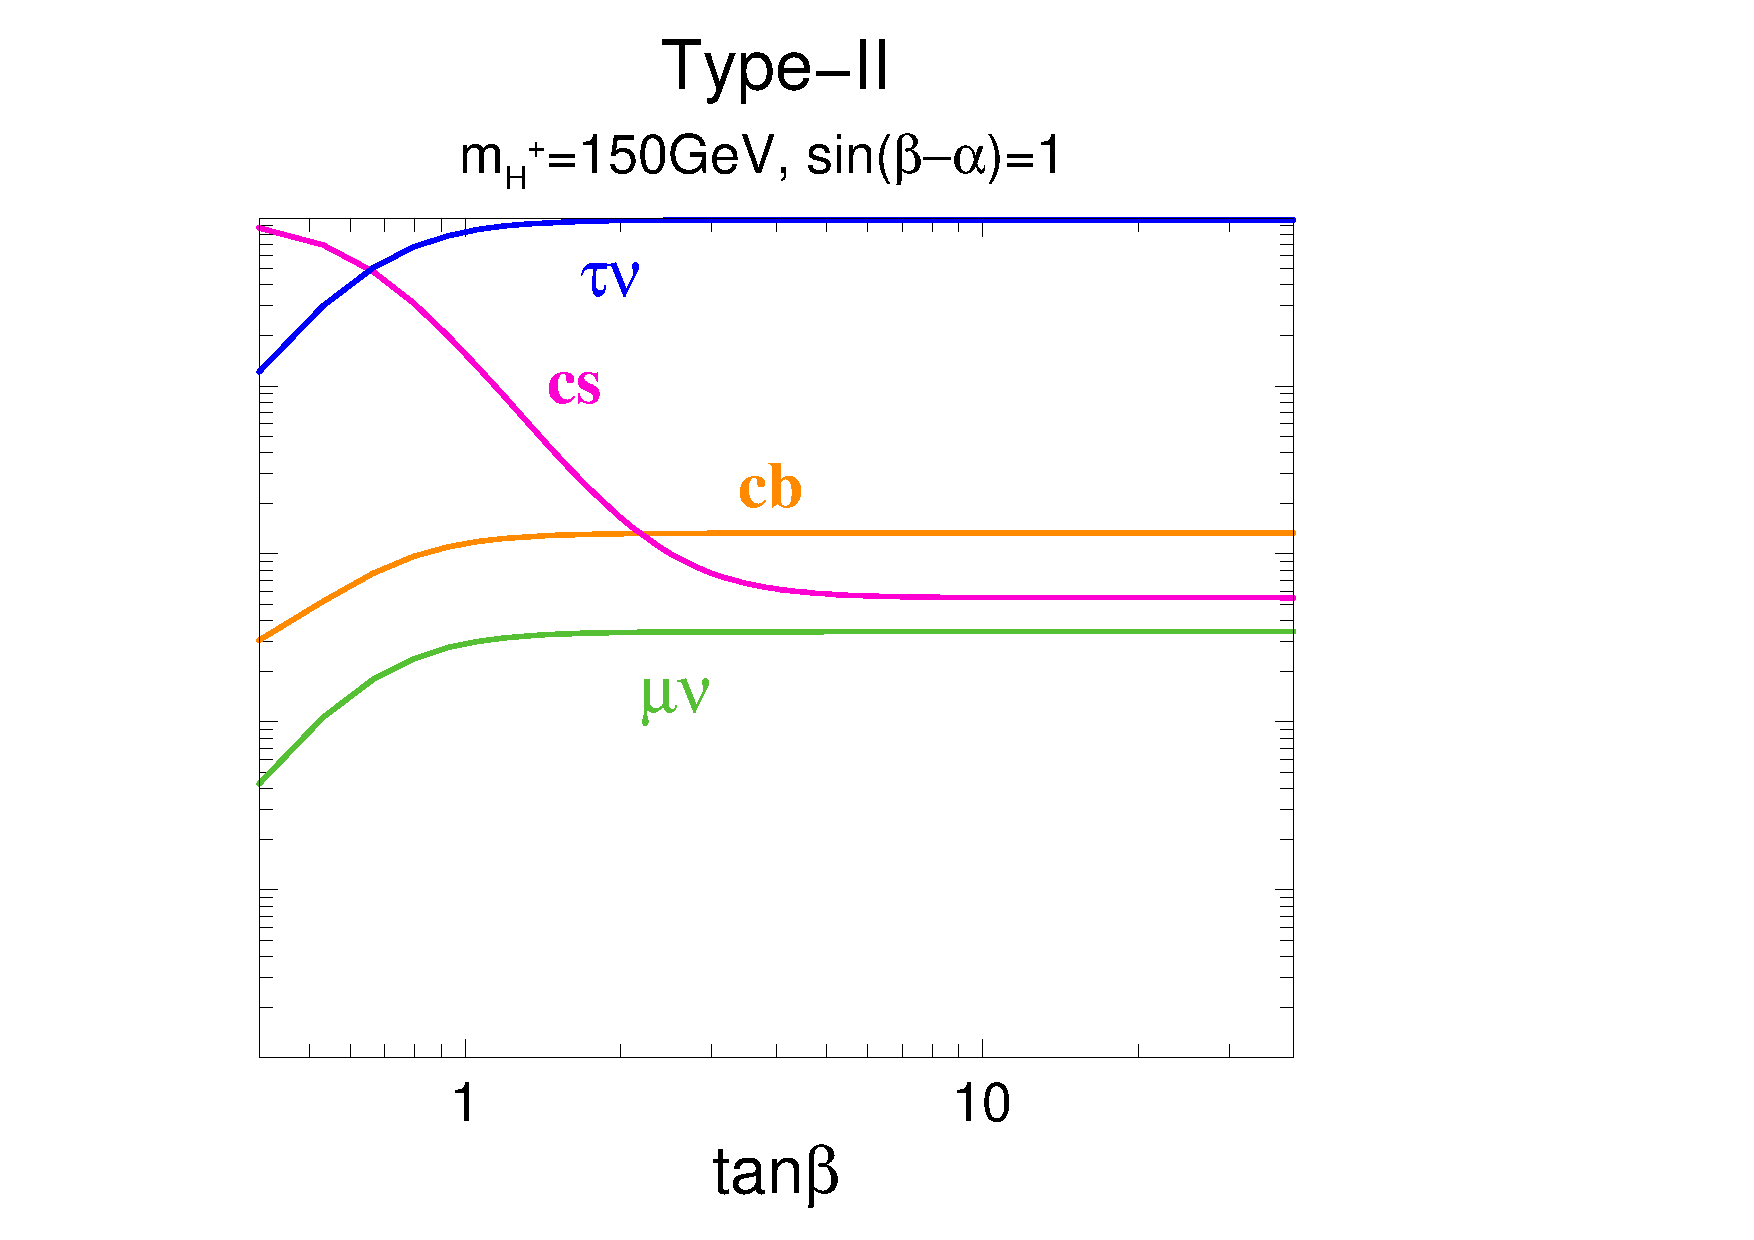
\includegraphics[width=1.7\linewidth]{Theory/Image/BR_ch_2.pdf}
%\end{minipage}
%\begin{minipage}{0.24\hsize}
%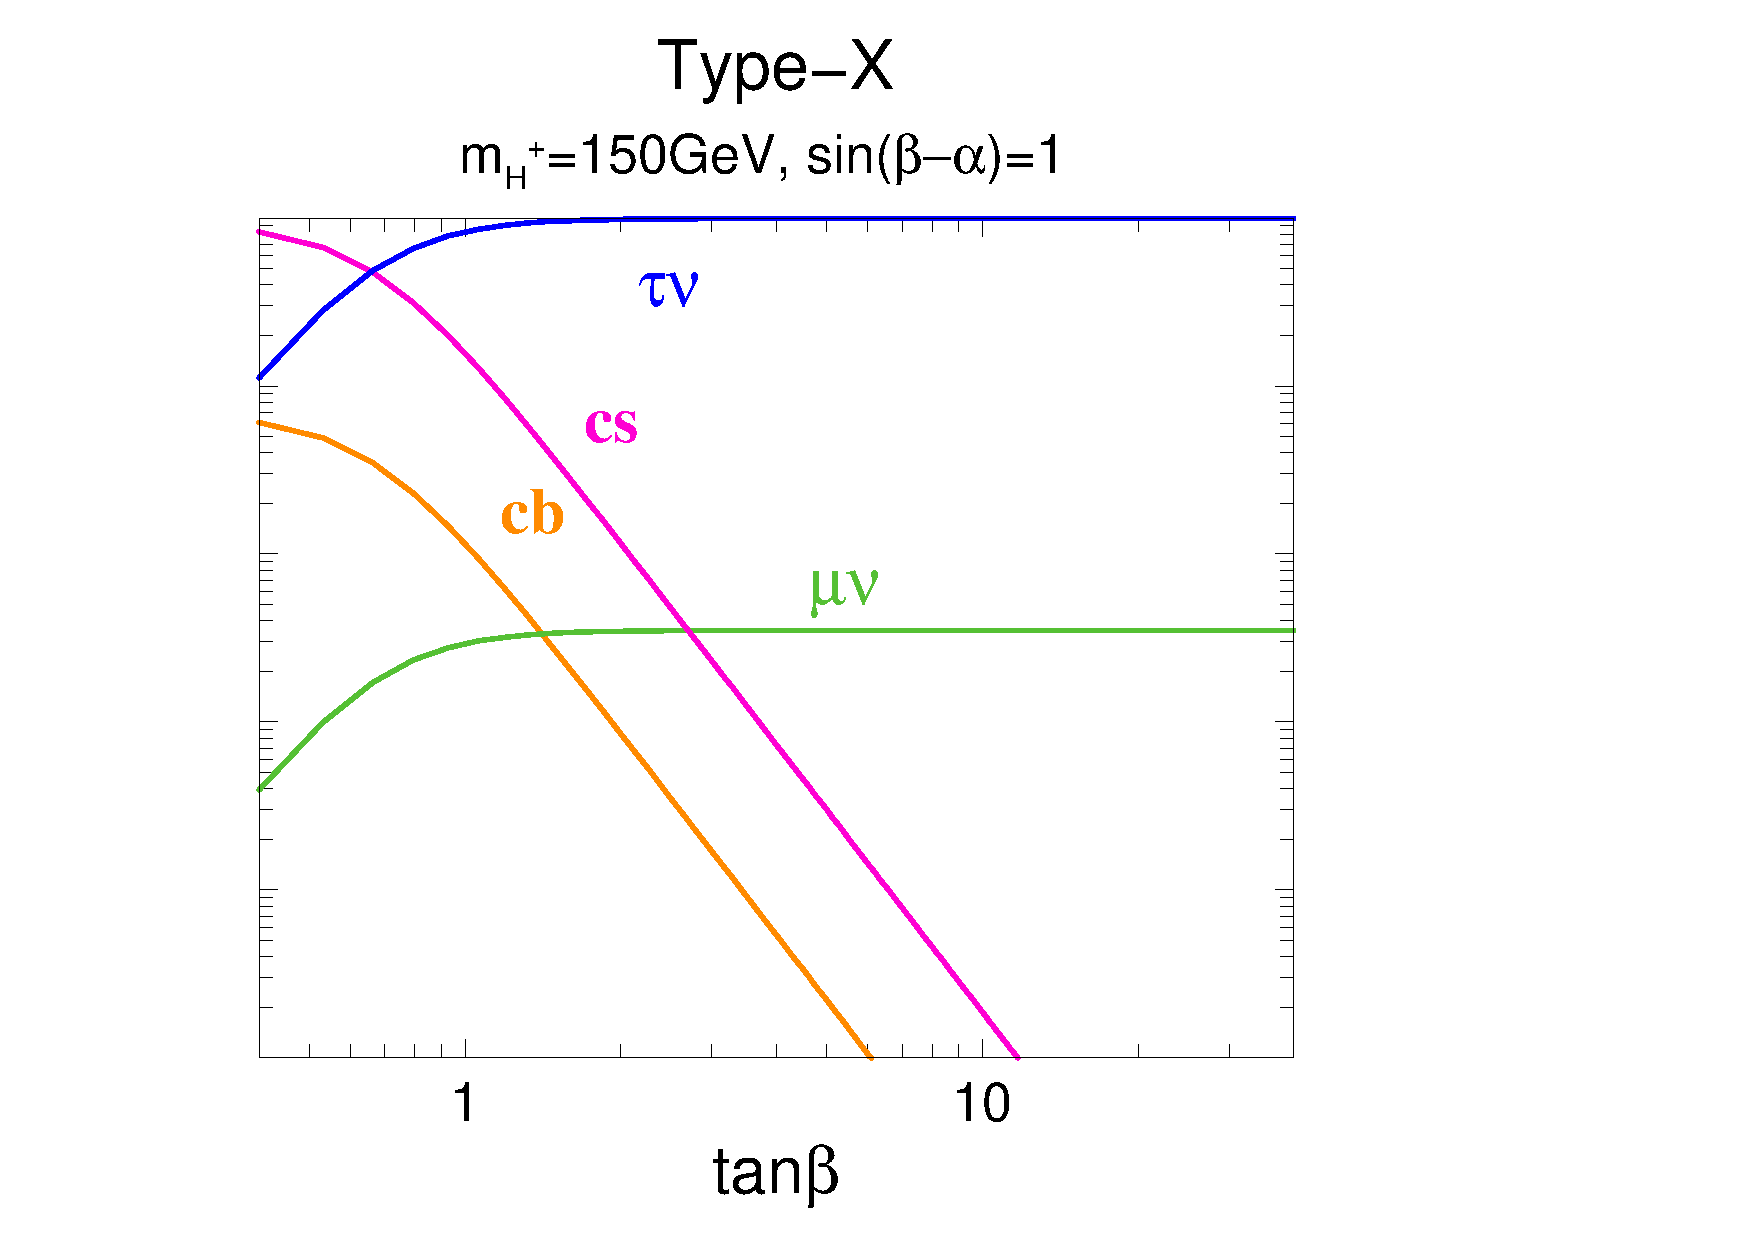
\includegraphics[width=1.7\linewidth]{Theory/Image/BR_ch_X.pdf}
%\end{minipage}
%\begin{minipage}{0.24\hsize}
%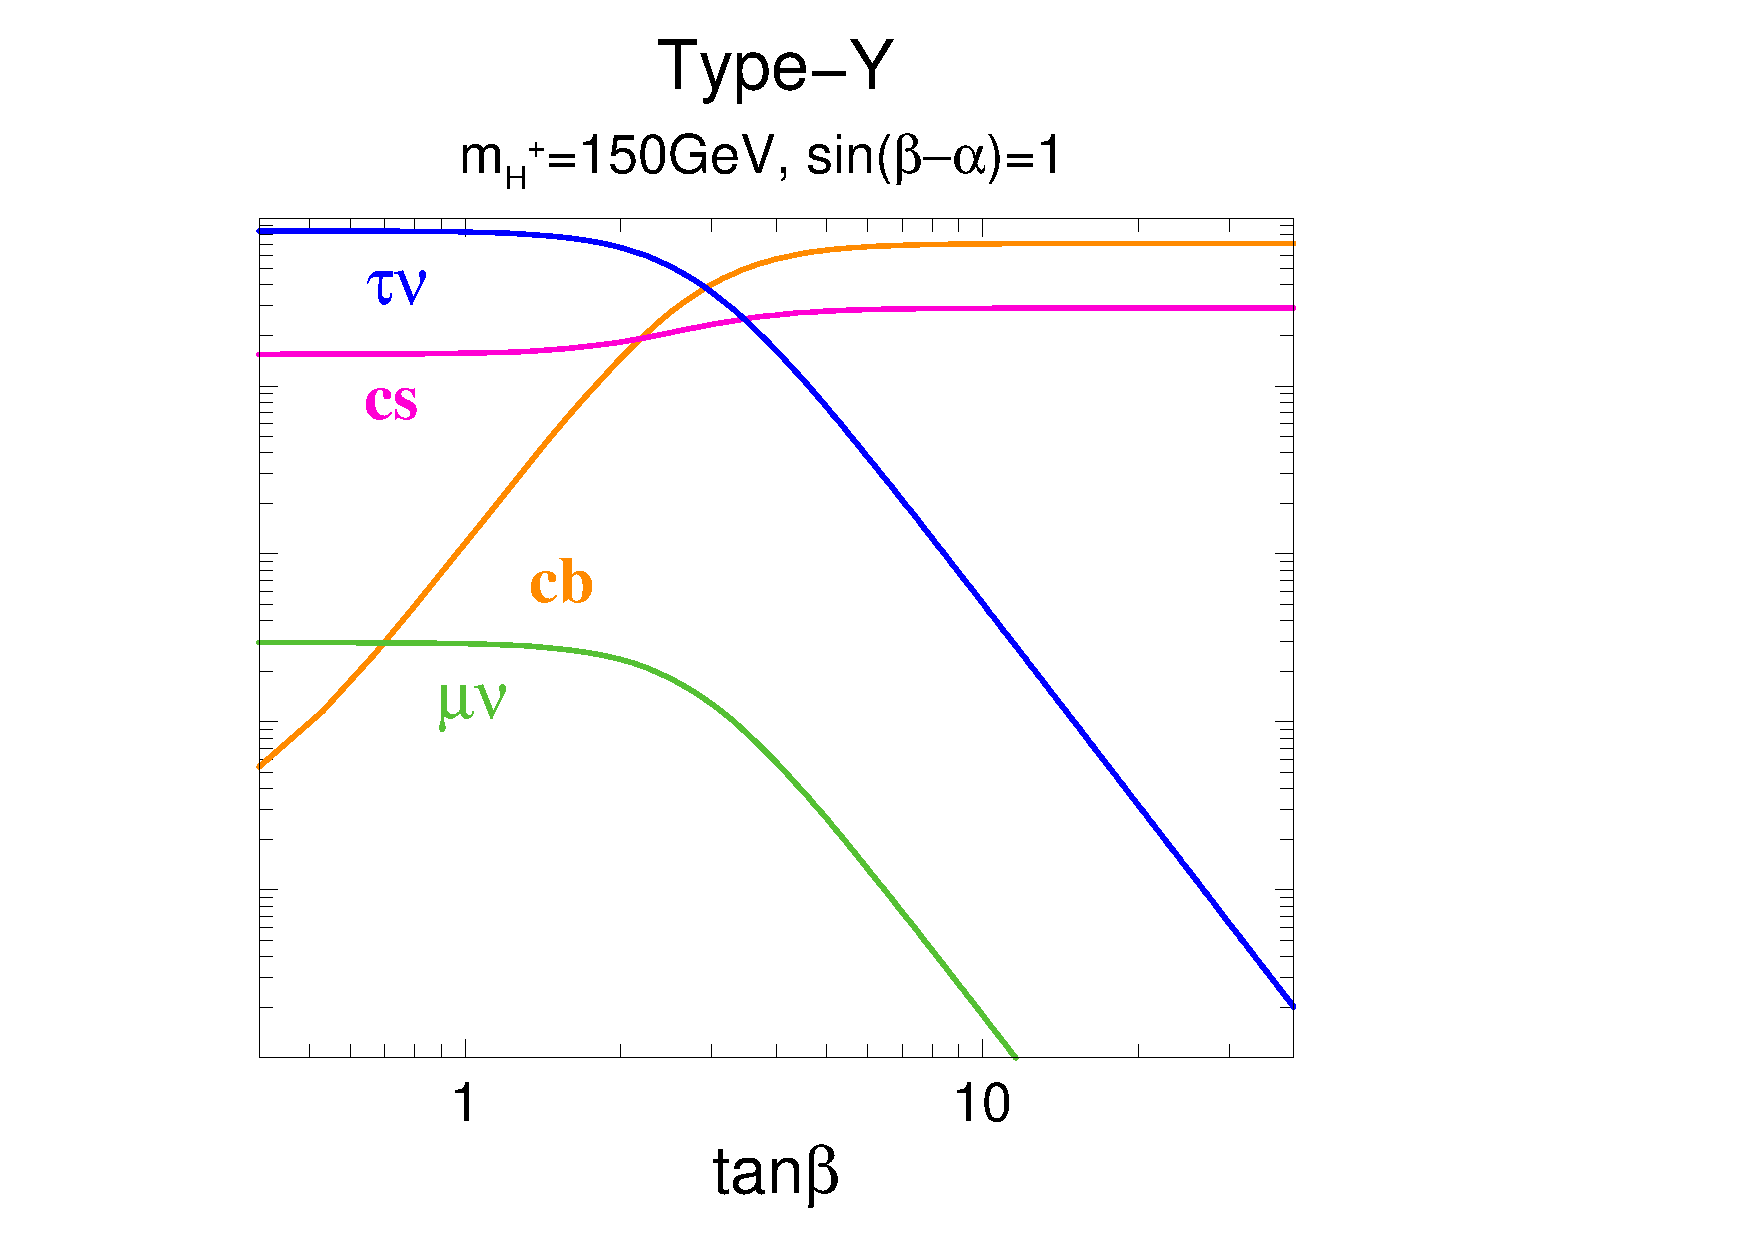
\includegraphics[width=1.7\linewidth]{Theory/Image/BR_ch_Y.pdf}
%\end{minipage}
%\caption{Decay branching ratios of $H$, $A$ and $H^\pm$
%in the four different types of THDM as a function of $\tan\beta$
%for $m_H^{}=m_A^{}=m_{H^\pm}^{}=150$ GeV and $M=149$ GeV.
%The SM-like limit $\sin(\beta-\alpha) =1$ is taken, where $h$
%is the SM-like Higgs boson.}
%\label{FIG:br_150}
%\end{center}
%\end{figure}

\section{Branching ratio of top quark decay}
\label{s:brThb}
Being a very short-lived particle with a lifetime of $5\times 10^{-25}$\unit{s}, the
\PQt quark decays immediately. In the SM, it decays only to W boson
and \PQb quark as its decay involving other quarks (s, d) is suppressed
by the corresponding element of the CKM matrix. The ratio R = \brTwb/\brTwq 
where q = \PQb, \PQs, and \PQd is 0.90 $\pm$ 0.04 as was earlier 
determined from D0 experiment using 5.4 $\fbinv$ 
data \cite{PhysRevLett.107.121802}. The CDF experiment using 162 
pb$^{-1}$ luminosity has put a lower bound at 95\% CL on it, 
R $>$ 0.61 \cite{PhysRevLett.95.102002}. The latest lower bound, R $>$ 
0.95, is obtained from the CMS experiment at 8 \TeV using 19.7\fbinv 
luminosity \cite{Khachatryan:2014nda}  which suggests that the \PQt 
quark can have other decay channels beyond the SM. In the 2HDM, it is allowed to 
decay into $H^+q$ channel. The branching ratio of this decay process is given by
\begin{equation}
BR(t\to H^+q) = \frac{\Gamma(t\to H^+q)}{\Gamma(t\to W^+q)+\Gamma(t\to H^+q)}
\label{eq:brThb}
\end{equation}
where $\Gamma(t\to H^+q)$ and $\Gamma(t\to W^+q)$ are the partial decay widths. 
For the \PQb quark, these decay widths are given as \cite{PhysRevD.80.015017}
\begin{align}
\Gamma(t\to H^+b) =&
\frac{G_F\left|V_{tb}\right|^2}{8\sqrt2\pi m_t}
\lambda\left(\frac{m_b^2}{m_t^2},\frac{m_{H^\pm}^2}{m_t^2}\right)^{1/2}
\nonumber\\
&\times
\left\{m_t^2\left[m_t^2{G_A^u}^2\left(1+\frac{m_b^2}{m_t^2}-\frac{m_{H^\pm}^2}{m_t^2}\right)+m_b^2{G_A^d}^2\right]
+4m_t^2m_b^2G_A^uG_A^d\right\},
\end{align}
and 
\begin{equation}
\Gamma(t\to W^+b) = \frac{G_F\left|V_{tb}\right|^2}{8\sqrt2\pi}m_t^3
\end{equation}
where
\begin{equation}
\lambda(x,y) = 1+x^2+y^2-2x-2y-2xy,
\end{equation}
and \mt = 166 \GeV (running mass of the \PQt quark), $m_b$ (running mass of \PQb quark) = 3.0 \GeV, $G_{F}$ = 
$1.1663\times 10^{-5}$, and $V_{tb}$ = 0.99. The variation of \brThb as 
a function of $\tan\beta$ and the mass of the charged Higgs is shown in Figure~\ref{fig:brThb}. 
From the plots shown on the left side, it can be seen that for low $\tan\beta < 1$, the $\brThb$ is 
the same for all the types 
of 2HDM. For higher $\tan\beta$, the \brThb increases in the Type II model as compared to Type X.
The similar $\tan\beta$ dependence can be explicitly seen from the right hand plots of this figure. 
Please note that \brThb is the same for Type I and X, and for Type II and Y as the coupling 
of quarks with charged Higgs is same as shown in Table~\ref{tab:coupling2HDM}. 
We also see that \brThb does not change much with respect to the mass of charged Higgs
for \mHp $<$ 150 \GeV.

\begin{figure}
\centering  
\subfigure[]
	{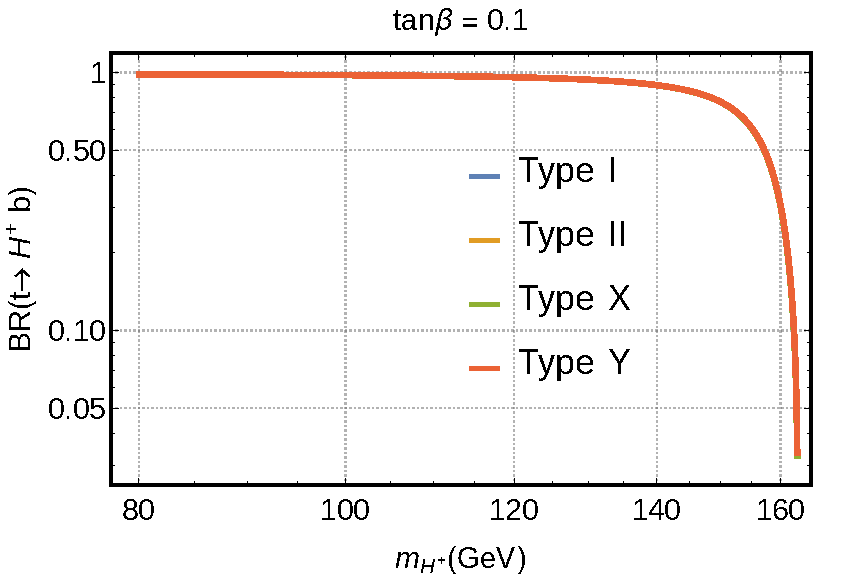
\includegraphics[width=0.45\linewidth]{Theory/Image/BR_topToHb_b0p1.pdf}}
\subfigure[]
	{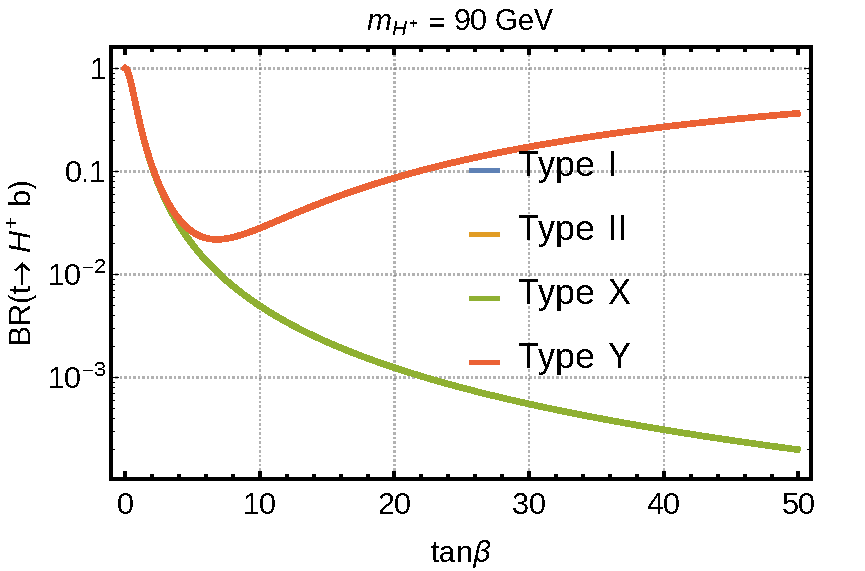
\includegraphics[width=0.45\linewidth]{Theory/Image/BR_topToHb_mH90.pdf}}
\vfil
\subfigure[]
	{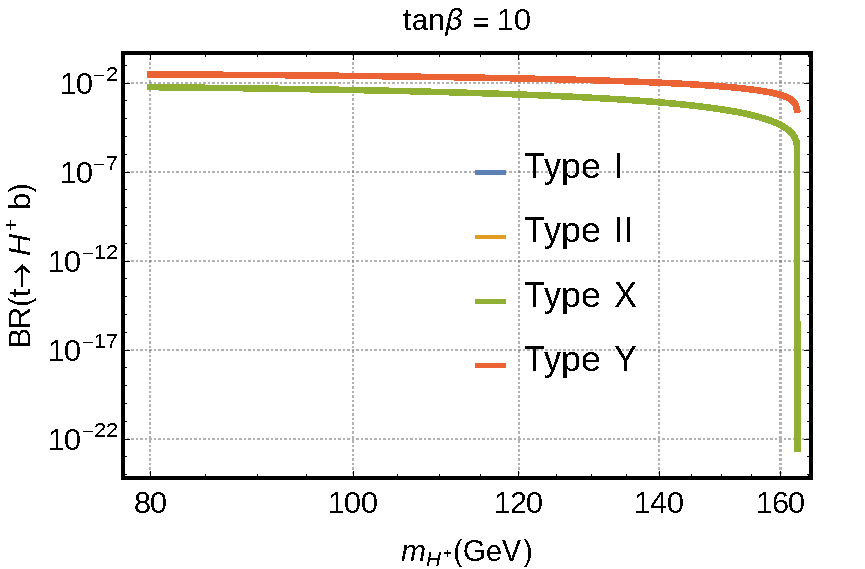
\includegraphics[width=0.45\linewidth]{Theory/Image/BR_topToHb_b10.pdf}}
\subfigure[]
	{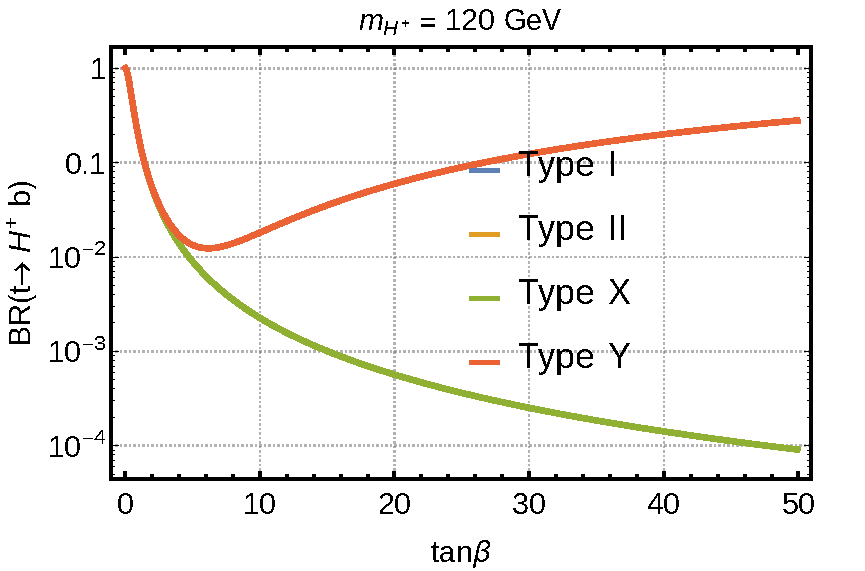
\includegraphics[width=0.45\linewidth]{Theory/Image/BR_topToHb_mH120.pdf}}
\vfil
\subfigure[]
	{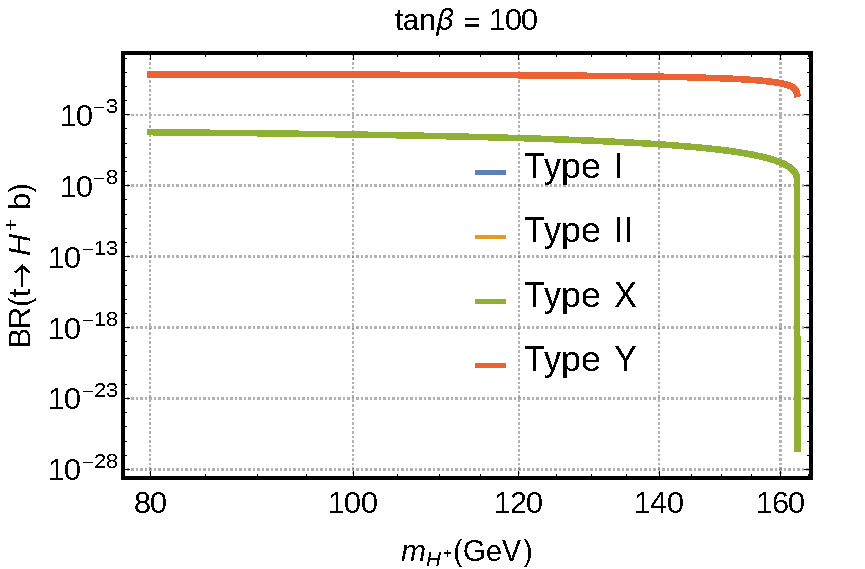
\includegraphics[width=0.45\linewidth]{Theory/Image/BR_topToHb_b100.pdf}}
\subfigure[]
	{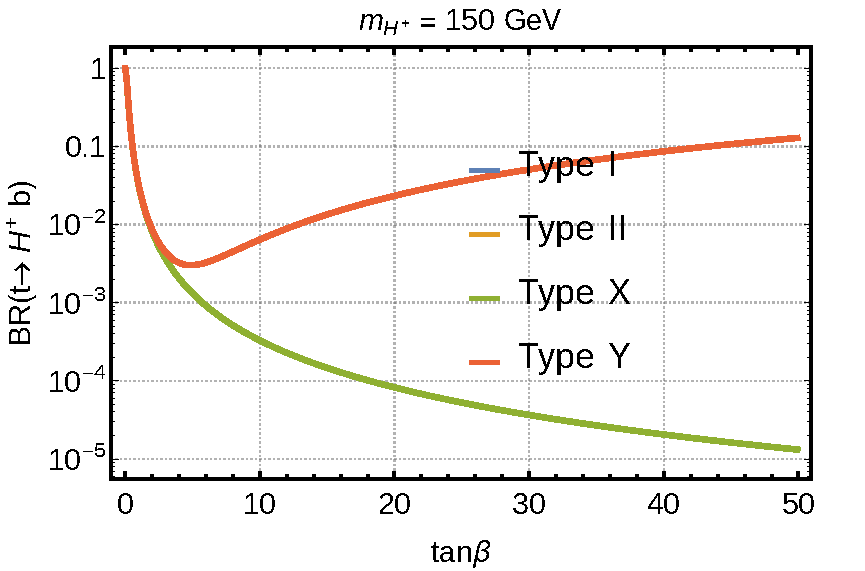
\includegraphics[width=0.45\linewidth]{Theory/Image/BR_topToHb_mH150.pdf}}
\caption{Variation of \brThb as a function of the mass of the charged Higgs 
	(left side plots) and $\tan\beta$ (right side plots).}
\label{fig:brThb}
\end{figure}

\section{Branching ratio of charged Higgs decay}
\label{s:brHqq}
For the search of charged Higgs boson, it is very important to study all of its 
possible decay channels to have an estimate of the dominance of respective
channels for a given value of $\tan\beta$, \mHp, etc. In the 2HDM, the charged
Higgs is allowed to decay into fermions and gauge bosons for example 
$H^+ \rightarrow c\bar{s}$, $H^+ \rightarrow c\bar{b}$, 
$H^+ \rightarrow t\bar{b}$, $H^+ \rightarrow \tau^+\nu_\tau$, 
$H^+ \rightarrow W^+\gamma$, $H^+ \rightarrow W^+Z$, $H^+ \rightarrow hW^+$, 
$H^+ \rightarrow HW^+$, and $H^+ \rightarrow AW^+$. The partial decay width of charged 
Higgs decaying to quarks and leptons is given by \cite{PhysRevD.80.015017}
\begin{align}
\Gamma(H^+\to u{\bar d}) = N_C
\frac{G_Fm_{H^\pm}^{}\left|V_{ud}\right|^2}{4\sqrt2\pi}\beta_{ud}^{}
\left\{\left(m_u^2{G^u_A}^2+m_d^2{G^d_A}^2\right)
\left(1-\frac{m_u^2+m_d^2}{m_{H^\pm}^2}\right)-\frac{4m_u^2m_d^2
{G^u_A}{G^d_A}}{m_{H^\pm}^2}\right\},
\label{Eq:H+ud}
\end{align}
and 
\begin{align}
\Gamma(H^+\to \ell^+\nu) =
\frac{G_Fm_{H^\pm}^{}m_\ell^2}{4\sqrt2\pi}{G^\ell_A}^2
\left(1-\frac{m_\ell^2}{m_{H^\pm}^2}\right)^2
\label{Eq:H+nul}
\end{align}
where 
\begin{align}
\beta_{XY}^{} &= \lambda^{1/2}\left(\frac{m_X^2}{m_\varphi^2},
\frac{m_Y^2}{m_\varphi^2}\right),
\end{align}
and $ N_C = 3, ~V_{cs} = 0.97, ~m_c = 0.81$ \GeV, $m_s = 0.046$ \GeV, $V_{cb} = 
0.0412, ~m_\tau = 1.77$ \GeV, $m_\mu = 0.105$ \GeV. The total decay width of charged
Higgs decay is given by
\begin{align}
\Gamma(H^+\to \rm{All}) = \Gamma(H^+\to \tau^+\nu) + \Gamma(H^+\to c\bar{s}) + 
\Gamma(H^+\to c\bar{b}) + \Gamma(H^+\to \mu^+\nu))
\end{align}
The branching ratio of charged Higgs decay into different channels is shown in
Figure~\ref{fig:brHqq}. As shown in this figure, the $\tau^+\nu$ channel is
dominant for all $\tan\beta$ in the Type I model. For low $\tan\beta$, the 
$c\bar{s}$ channel is dominant in Type II and Type X. 
\begin{figure}
\centering  
\subfigure[]{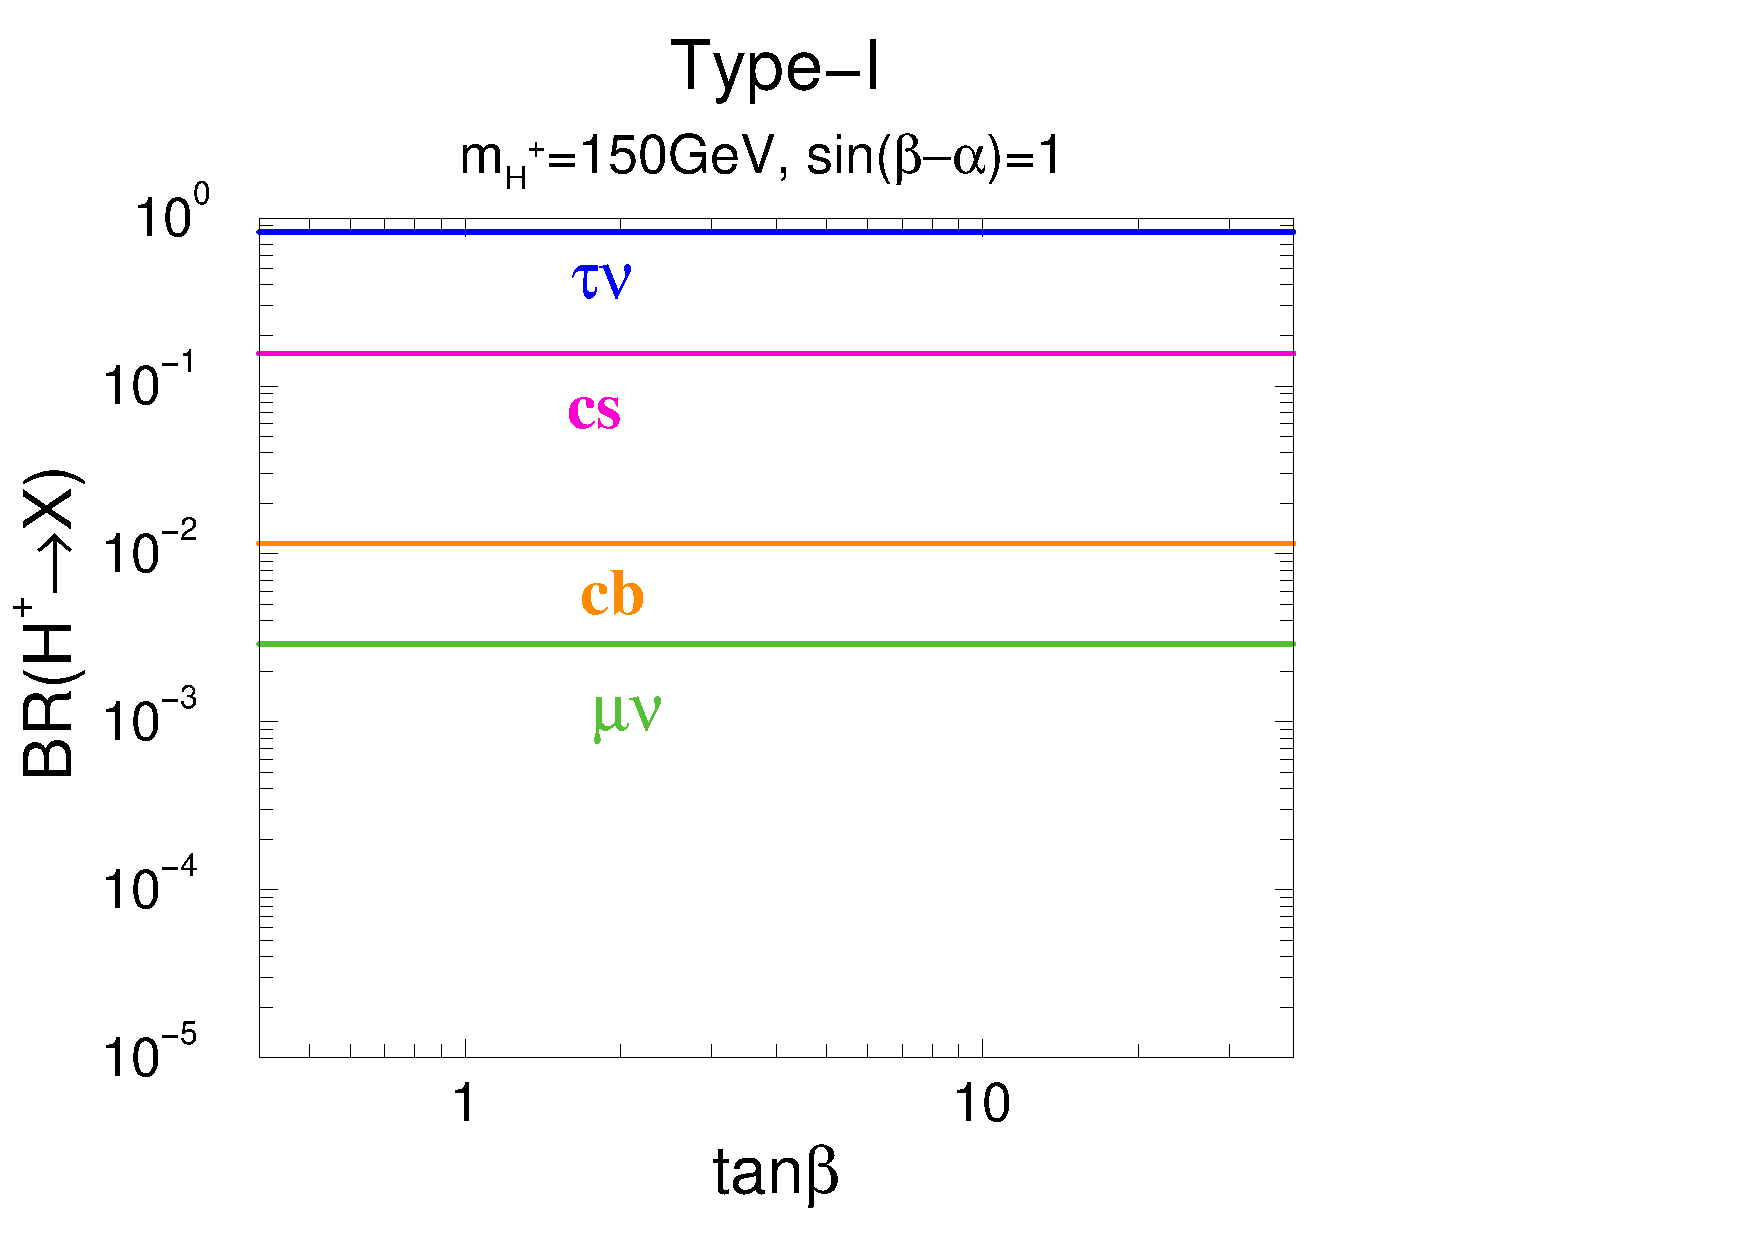
\includegraphics[width=0.49\linewidth]{Theory/Image/BR_ch_1.pdf}}
\subfigure[]{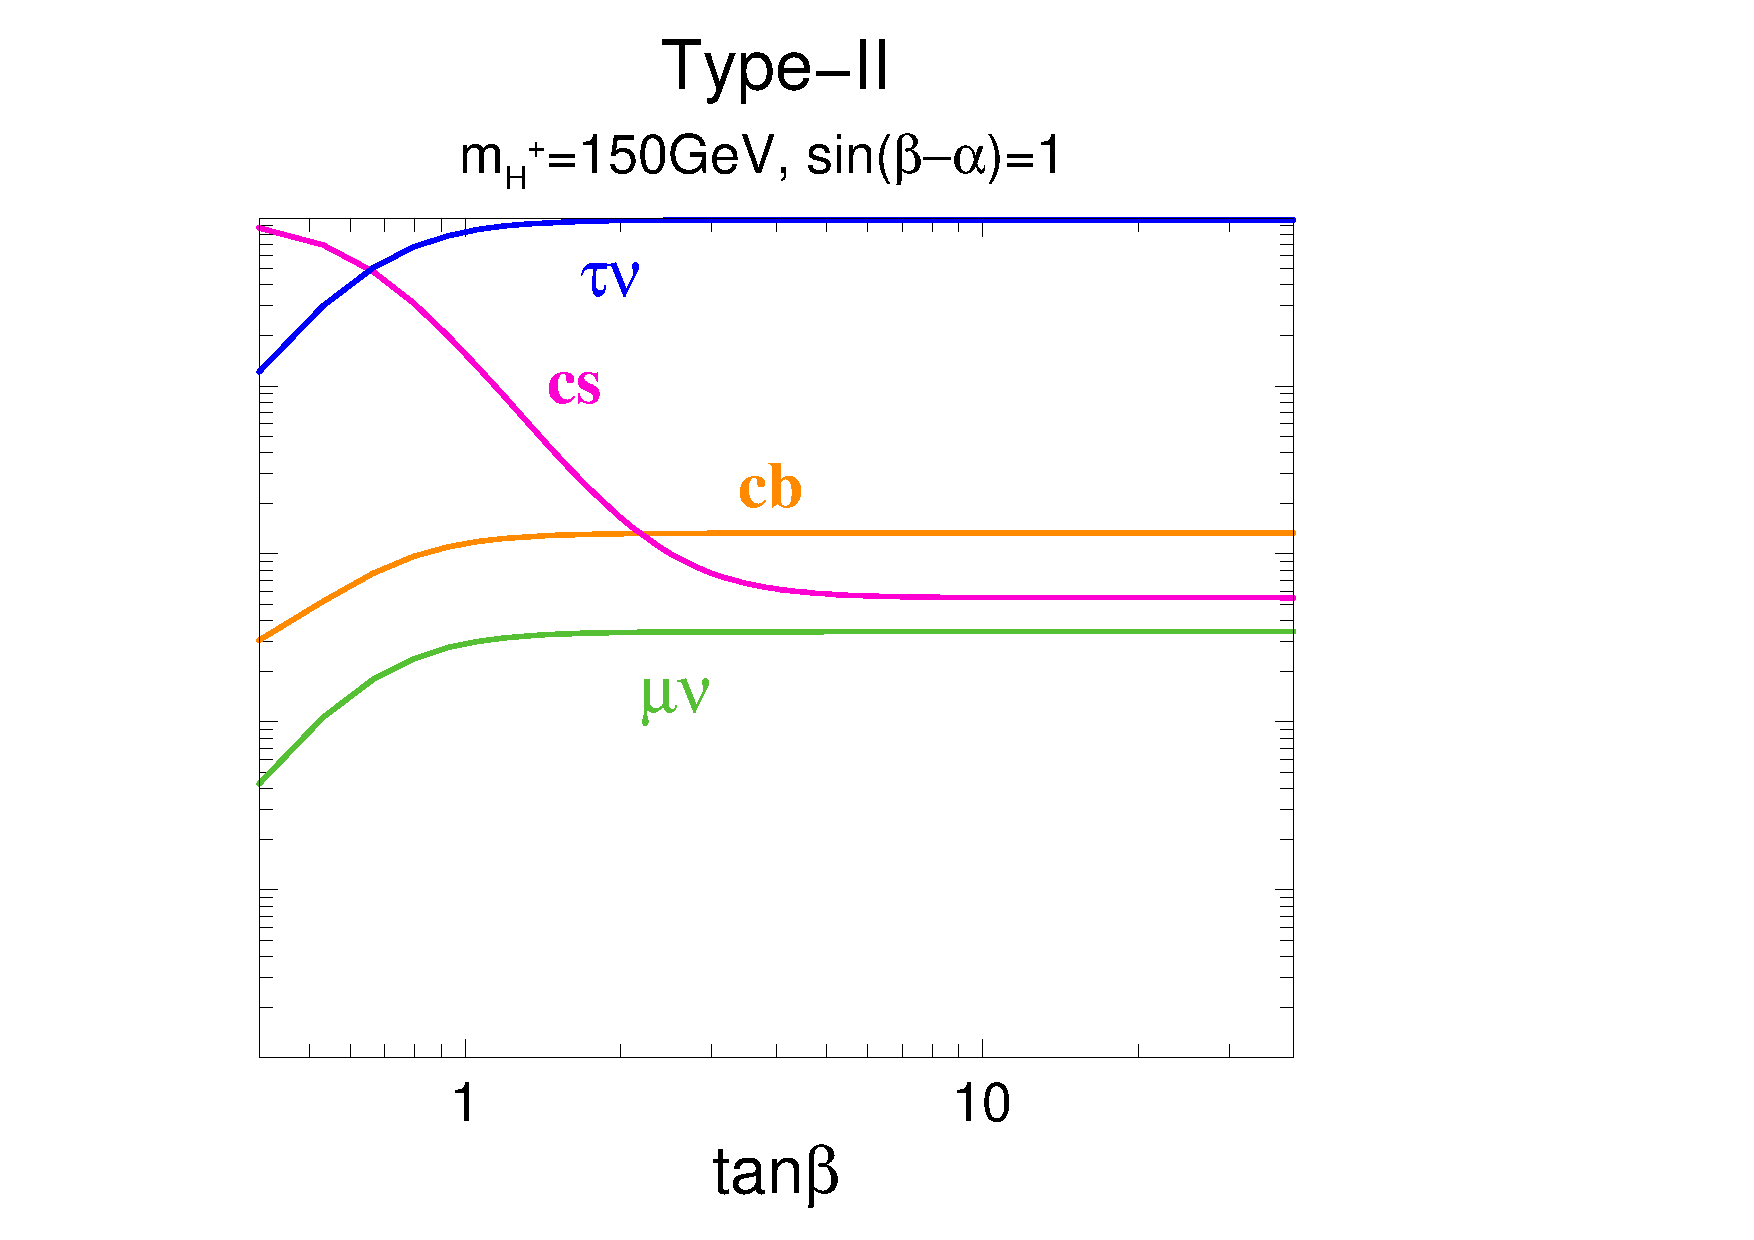
\includegraphics[width=0.49\linewidth]{Theory/Image/BR_ch_2.pdf}}
\vfil
\subfigure[]{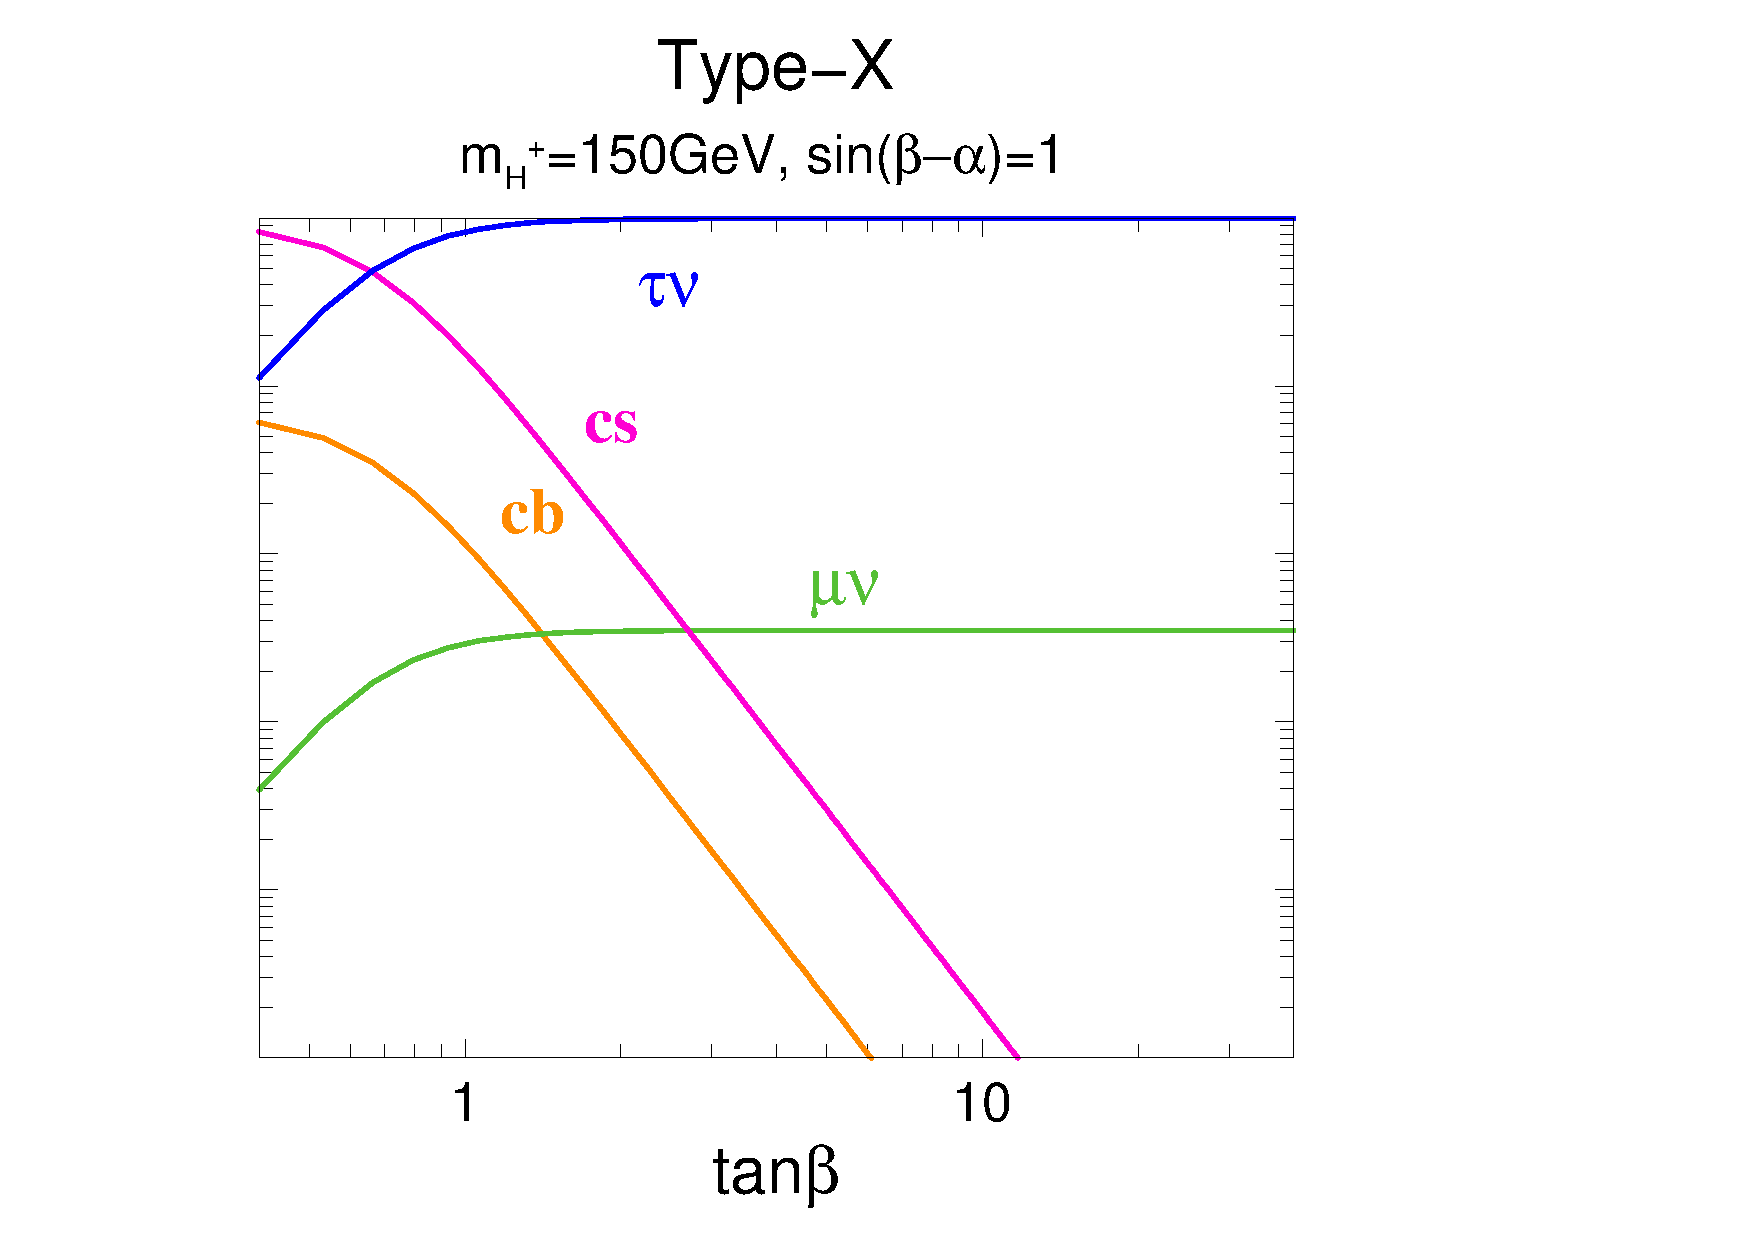
\includegraphics[width=0.49\linewidth]{Theory/Image/BR_ch_X.pdf}}
\subfigure[]{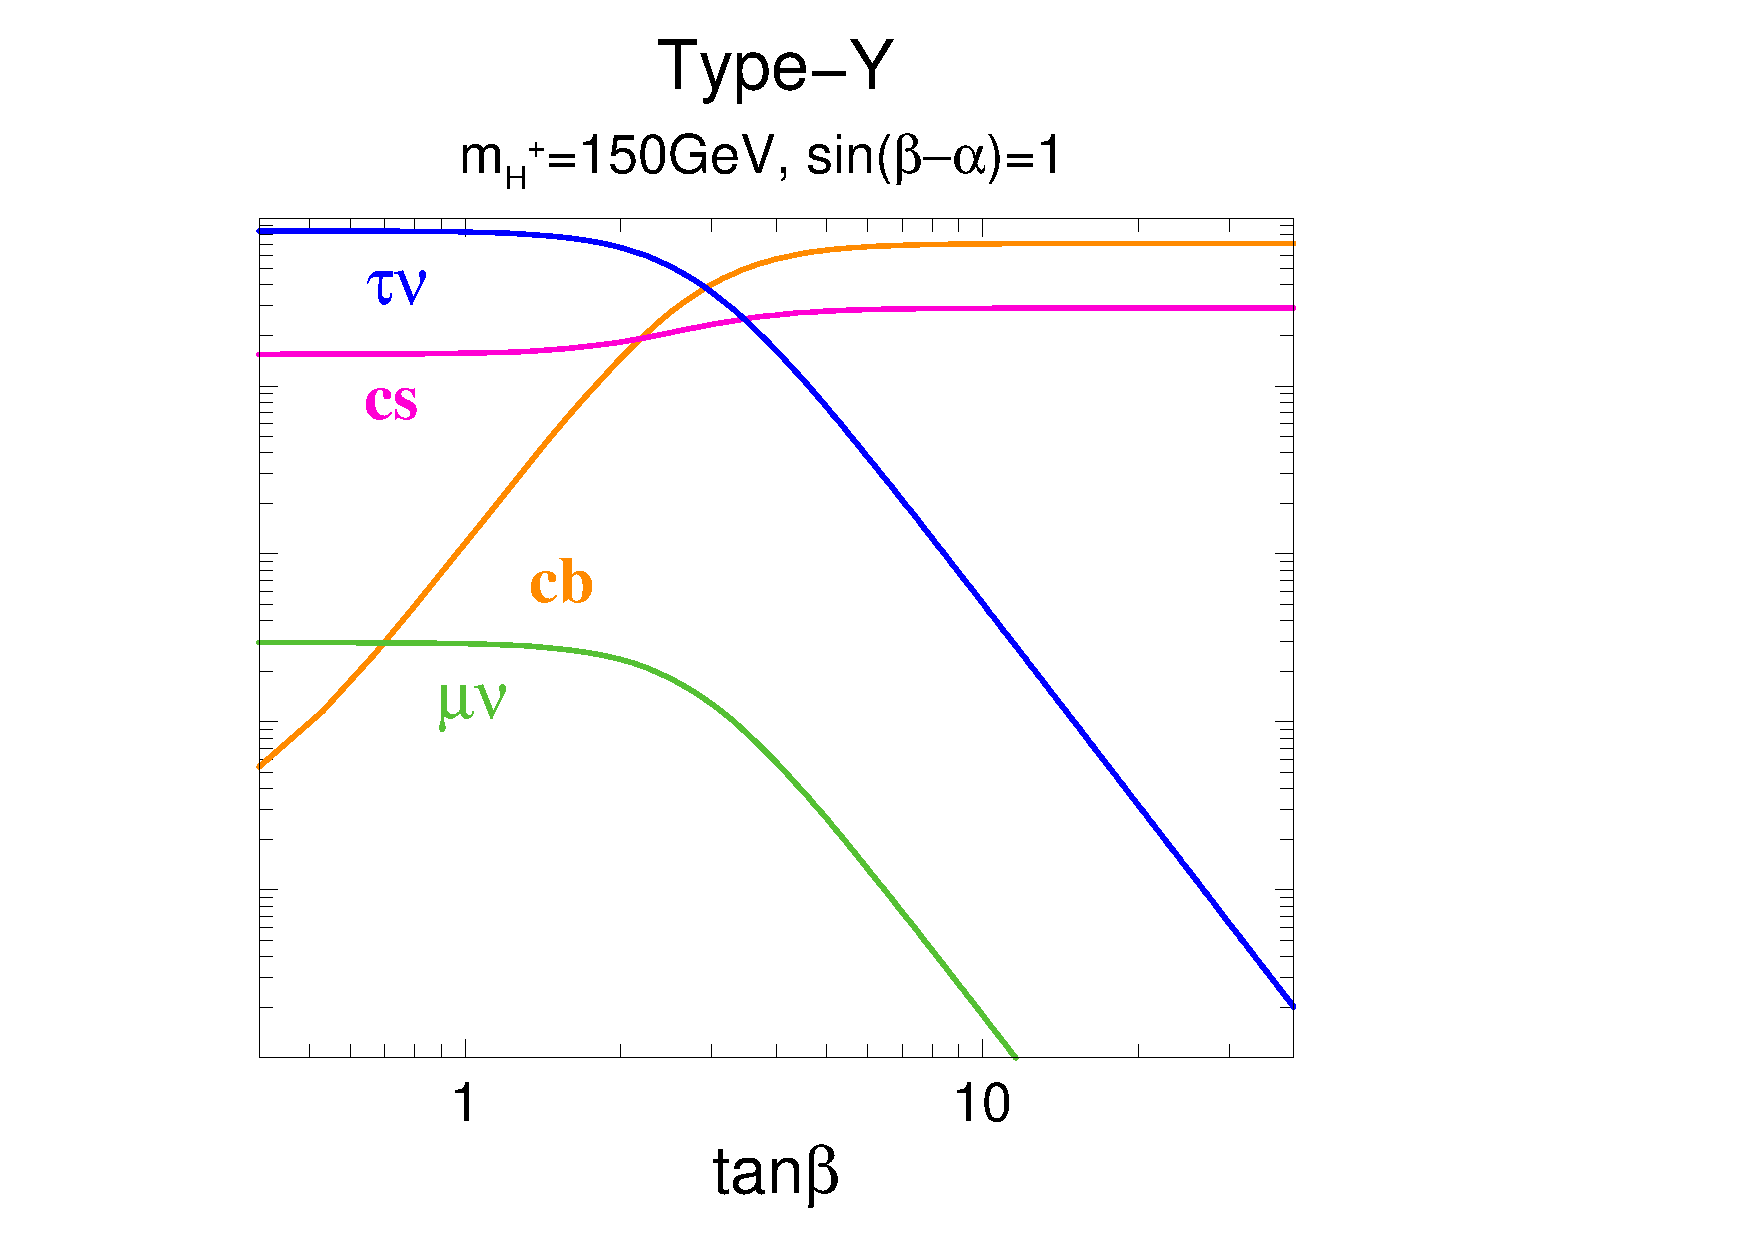
\includegraphics[width=0.49\linewidth]{Theory/Image/BR_ch_Y.pdf}}
\caption{The branching ratio of charged Higgs decay in different channels
	 as a function of $\tan\beta$ for $\mHp$ = 150 \GeV in 
	different types of the 2HDM. These plots are taken from \cite{PhysRevD.80.015017}. }
\label{fig:brHqq}
\end{figure}


\section{Current status of searches for charged Higgs}
\label{s:searchHplus}
There have been several searches for the charged Higgs boson in last two decades, 
particularly in the context of Type II of the 2HDM. However, no signature of the 
existence of the charged Higgs has been found
as of now. In the absence of any signal for the charged Higgs, various constraints
have been imposed from a wide range of theoretical studies as well as low and high energy 
collider experiments. The theoretical constraints come from the vacuum stability,
perturbative unitarity, and electro-weak precision observables 
\cite{Arhrib:2018ewj}. The low energy constraints are from the indirect searches
\cite{Akeroyd:2016ymd} where a charged Higgs appears in the loop such as the 
decay of B-mesons ($B \rightarrow X_s\gamma$). The high energy constraints are 
from the direct production of charged Higgs at the collider experiments 
\cite{Achard:2003gt, Heister:2002ev, Abdallah:2003wd, Abbiendi:2008aa,
Aaltonen:2009ke,Abazov:2009aa,Aad:2013hla,Khachatryan:2015uua}. The constraints 
from direct searches are more reliable as compared to those from indirect searches 
or theoretical predictions.

The direct searches of the charged Higgs have been performed at the different
experiments such as ALEPH, L3, DELPHI, and OPAL at the large electron-positron 
collider (LEP), D0 and CDF at the Tevatron, and finally CMS and ATLAS at the large hadron
collider (LHC) in different decay channels of the charged Higgs. These searches
have been performed at different center of mass energies, different luminosities,
and for a wide range of the mass of the charged Higgs boson. Constraints have
been imposed on various parameters such as the mass of charged Higgs, $\tan\beta$, 
branching ratio of \PQt quark decay into the charged Higgs and \PQb quark, etc. A 
summary of all constraints from the collider experiment is shown in Tables 
\ref{tab:searchHplus1} and \ref{tab:searchHplus2}. The current best constraints 
are: \mHp $\textgreater$ 79.3 \GeV from the ALEPH at 0.2 \TeV (0.63\fbinv), 
\brThb $\textless$ 0.8-0.5\% for \mHp in range 90 to 150 \GeV at 13 \TeV 
(35.9\fbinv) from the CMS experiment, \sigHp $\times$ \brHtv $\textless$ 
4.2-0.0025\unit{pb} for \mHp in range 90 to 2000 \GeV at 13 \TeV (36.1\fbinv) from 
the ATLAS, \sigHp $\times \mathcal{B}(\text{H}^+ \rightarrow \text{t}\bar{\text{b}})$  $\textless$ 
9.6-0.01\unit{pb} for \mHp in range 200 to 3000 \GeV at 13 \TeV (35.9\fbinv) from 
the CMS, and $\tan\beta < $ 1 values are excluded for all \mHp up to 
160 \GeV from both CMS as well as ATLAS. A few of the current best constraints 
are shown in Figure~\ref{fig:searchHplus}.
\begin{table}
	\caption{Allowed range at 95\% CL for various parameters from the search 
	for charged Higgs involving $c\bar{s}$ channel at different collider 
	experiments.}
	\label{tab:searchHplus1}
\begin{centering}
\begin{tabular}{ccp{3cm}p{5cm}p{3cm}}
	\hline
	\hline
	Experiment & Year & $\sqrt{s}$ ($\lumi_{int}$) & Allowed range at 95\% CL
	& Assumption \\ \noalign{\vskip 0.2cm} 
	& 	& \TeV (\fbinv)    &  	&\\
	\hline
	\hline \noalign{\vskip 0.2cm}
	ALEPH 	& 2002 \cite{Heister:2002ev} & 0.189-0.209 (0.629) & \mHp 
	$\textgreater$ 79.3 \GeV  & 
	\brHtv + \brHcs = 1\\ \noalign{\vskip 0.2cm}
	L3 	& 2003 \cite{Achard:2003gt} & 0.189-0.209 (0.629) & \mHp 
	$\textgreater$ 76.5 \GeV  & 
	\brHtv + \brHcs = 1\\ \noalign{\vskip 0.2cm}
	DELPHI 	& 2004 \cite{Abdallah:2003wd} & 0.189-0.209 (0.220) & \mHp 
	$\textgreater$ 74.5 \GeV  & 
	Pair production of $ H^+H^-$ in channels 
	$\tau^+\nu_\tau\tau^-\bar{\nu}_\tau, ~c\bar{s}\bar{c}s, 
	~c\bar{s}\tau^-\bar{\nu}_\tau$
	\\ \noalign{\vskip 0.2cm}
	OPAL 	& 2012 \cite{Abbiendi:2008aa} & 0.189-0.209 (0.6) & \mHp 
	$\textgreater$ 76.3 \GeV & 
	\brHtv + {\ensuremath{\mathcal{B}(H^+ \rightarrow \text{q}\text{q}^\prime)}\xspace} = 1
	\\ \noalign{\vskip 0.2cm}
	\hline
	CDF 	& 2009 \cite{Aaltonen:2009ke}& 1.96 (2.2) & \brThb $\textless$ 
	10-30\%, for \mHp in 
	range 60 to 150 \GeV& \brHcs = 1\\ \noalign{\vskip 0.2cm}
	D0 	& 2009 \cite{Abazov:2009aa} & 1.96 (1.0) & \brThb $\textless$ 
	22\%, for \mHp in 
	range 80 to 155 \GeV& \brHcs = 1\\ \noalign{\vskip 0.2cm}
	\hline
	ATLAS 	& 2013 \cite{Aad:2013hla} & 7 (4.7) & \brThb $\textless$ 5.1\%, 
	for \mHp in 
	range 90 to 150 \GeV& \brHcs = 1\\ \noalign{\vskip 0.2cm}
	CMS 	& 2016 \cite{Khachatryan:2015uua} & 8 (19.7) & \brThb $\textless$ 
	6.5-1.2\%, for \mHp in 
	range 90 to 150 \GeV& \brHcs = 1\\ \noalign{\vskip 0.2cm}
	CMS 	& 2019 & 13 (35.9) & \textcolor{red}{Presented in 
	this thesis} & \brHcs = 1\\ \noalign{\vskip 0.2cm}
	\hline
	\end{tabular}
	\par\end{centering}
\end{table}


\begin{table}
	\caption{Allowed range at 95\% CL for various parameters from the search 
	for charged Higgs involving other channels such as $\tau^+\nu, ~c\bar{b}$, 
	and $t\bar{b}$ at different collider experiments.}
	\label{tab:searchHplus2}
\begin{centering}
%\begin{tabular}{cccccc}
\begin{tabular}{ccp{2.0cm}p{6cm}p{3.5cm}}
	\hline
	\hline
	Experiment & Year & $\sqrt{s}$ ($\lumi_{int}$) & Allowed range at 95\% CL
	& Assumption \\ \noalign{\vskip 0.2cm} 
	& 	& \TeV (\fbinv)    &  	&\\
	\hline
	\hline \noalign{\vskip 0.2cm}
	D0 	& 2009 \cite{Abazov:2009aa} & 1.96 (1.0) & \brThb $\textless$ 
	15-19\%, for \mHp in range 80 to 155 \GeV& \brHtv = 1\\ \noalign{\vskip 0.2cm}
	ATLAS 	& 2013 \cite{Aad:2012rjx} & 7 (4.6) & \brThb $\textless$ 0.8-3.4\%, 
	for \mHp in range 90 to 160 \GeV& \brHtv = 1\\ \noalign{\vskip 0.2cm}
	ATLAS 	& 2015 \cite{Aad:2014kga} & 8 (19.5) & \sigHp$\times$\brHtv 
	$\textless$ 4.5-0.76\unit{pb} for \mHp in range 180 to 1000 \GeV, \brThb $\times$ 
	\brHtv $\textless$ 
	0.23-1.3\% for \mHp in range 80 to 160 \GeV, and $\tan\beta$ $\textless$ 
	1 for \mHp in range 80 to 160 \GeV& \brHtv = 1\\ \noalign{\vskip 0.2cm}
	ATLAS 	& 2016 \cite{Aaboud:2016dig} & 13 (3.2) & \sigHp $\times$ \brHtv 
	$\textless$ 1.9-0.015\unit{pb} for \mHp in range 200 to 2000 \GeV& \brHtv = 1\\ \noalign{\vskip 0.2cm}
	ATLAS 	& 2016 \cite{ATLAS:2016grc} & 13 (14.2) & \sigHp $\times$ \brHtv 
	$\textless$ 2.0-0.008\unit{pb} for \mHp in range 200 to 2000 \GeV& \brHtv = 1
	\\ \noalign{\vskip 0.2cm}
	ATLAS 	& 2018 \cite{Aaboud:2018gjj}& 13 (36.1) & \sigHp $\times$ \brHtv 
	$\textless$ 
	4.2-0.0025\unit{pb} for \mHp in range 90 to 2000 \GeV, \brThb $\times$ \brHtv 
	$\textless$ 0.25-0.031\% for \mHp in range 90 to 160 \GeV, and $\tan\beta$ 
	$\textless$ 1 is excluded for all \mHp up to 160 \GeV& \brHtv = 1
	\\ \noalign{\vskip 0.2cm}
	CMS 	& 2018 \cite{Sirunyan:2018dvm}& 8 (19.7) & \brThb $\textless$ 
	0.8-0.5\%, for \mHp in 
	range 90 to 150 \GeV& $\mathcal{B}(H^+\rightarrow \text{c}\bar{\text{b}})$ = 1\\ 
	\noalign{\vskip 0.2cm}
	CMS 	& 2019 \cite{Sirunyan:2019hkq}& 13 (35.9) & \sigHp $\times$ 
	\brHtv $\textless$ 
	6.0-0.005\unit{pb} for \mHp in range 80 to 3000 \GeV, and $\tan\beta$ $\textless$ 
	1 is excluded for all \mHp up to 160 \GeV& \brHtv = 1
	\\ \noalign{\vskip 0.2cm}
	CMS 	& 2019 \cite{CMS:1900zym} & 13 (35.9) & \sigHp $\times \mathcal{B} 
	(H^+\rightarrow t \bar{b})$ $\textless$ 9.6-0.01\unit{pb}, for \mHp in range 
	200 to 3000 \GeV & $\mathcal{B} (\text{H}^+\rightarrow \text{t} \bar{\text{b}})$ = 1
	\\ \noalign{\vskip 0.2cm}
	\hline
	\end{tabular}
	\par\end{centering}
\end{table}

\begin{figure}
\centering
\subfigure[Limit on \brThb \cite{Aad:2013hla}]{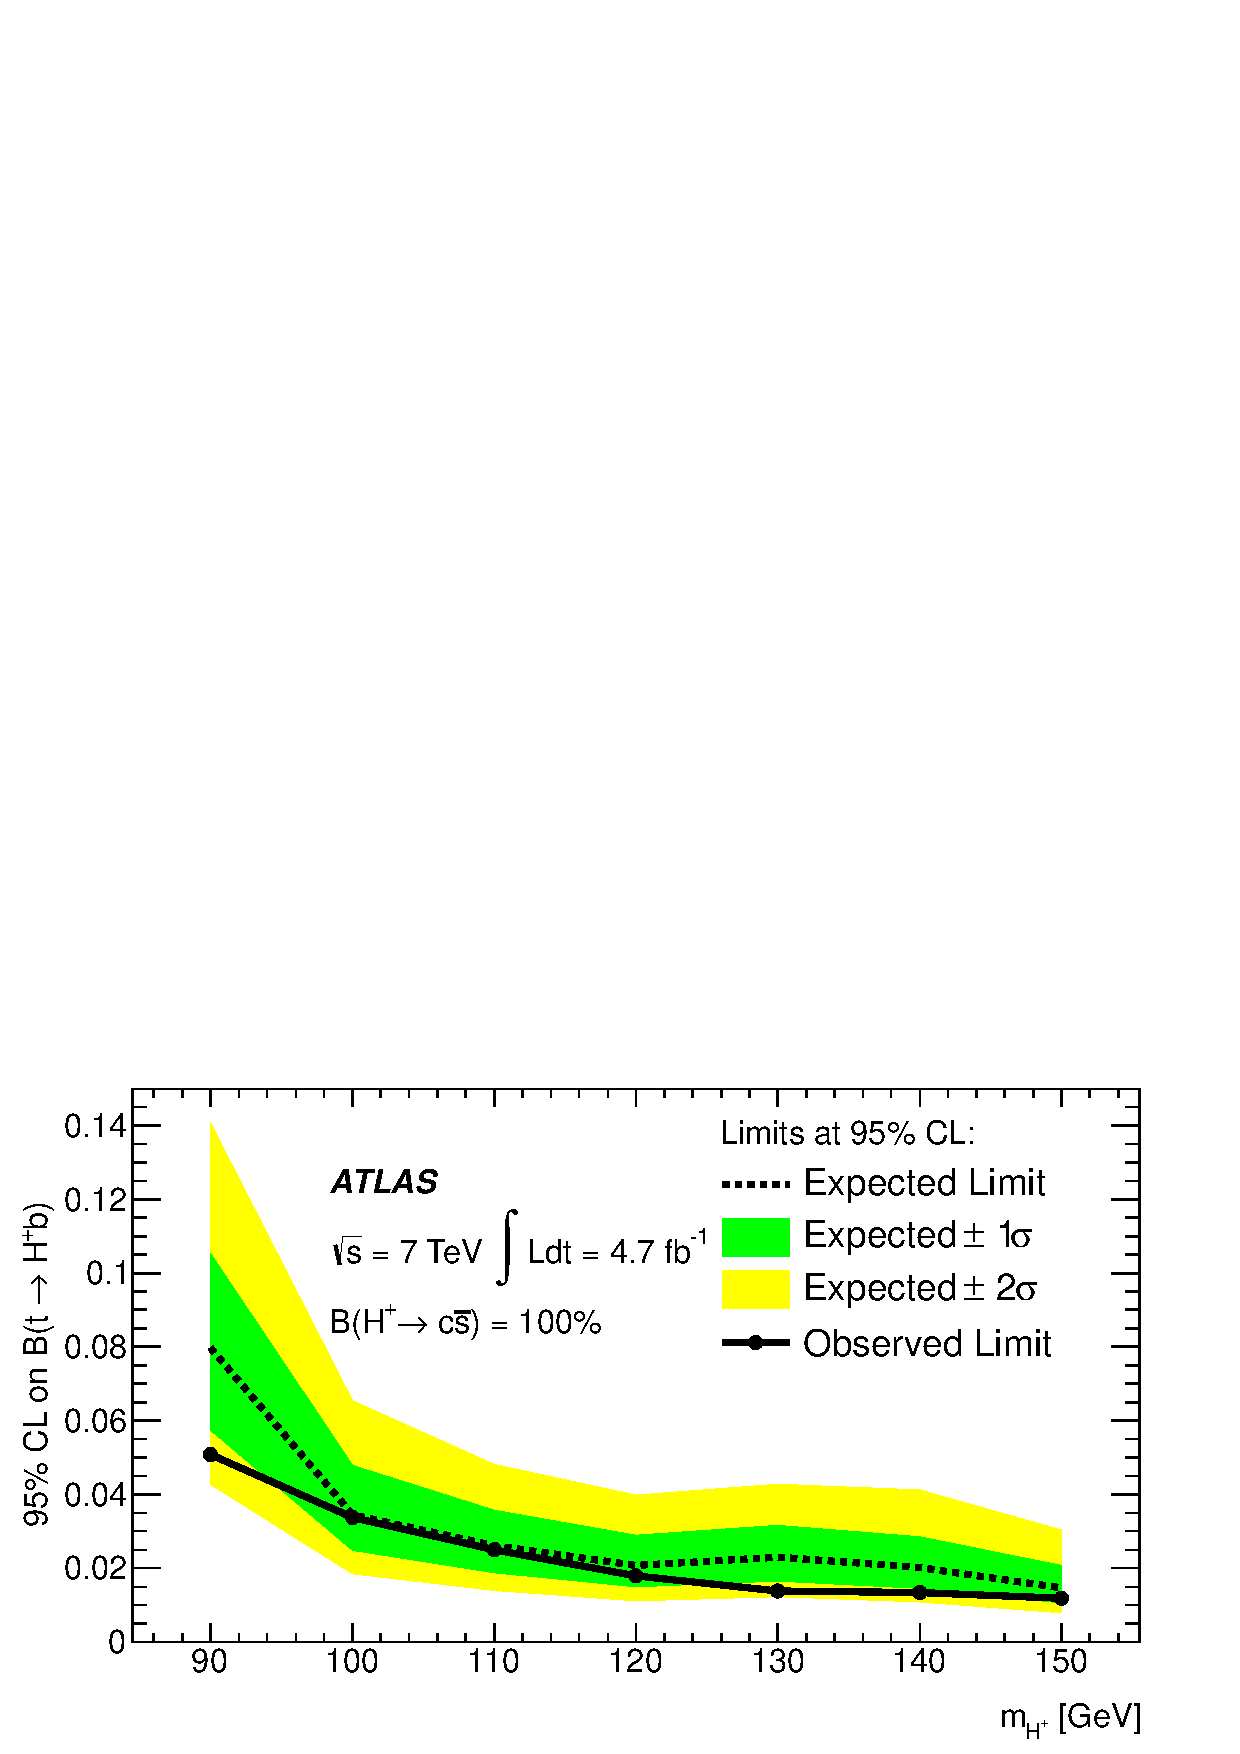
\includegraphics[width=0.50\linewidth]{Theory/Image/OldLimit/limit_atlas_csbar_7TeV.pdf}}
\subfigure[Limit on \sigHp$\times$\brHtv \cite{Aaboud:2018gjj}]{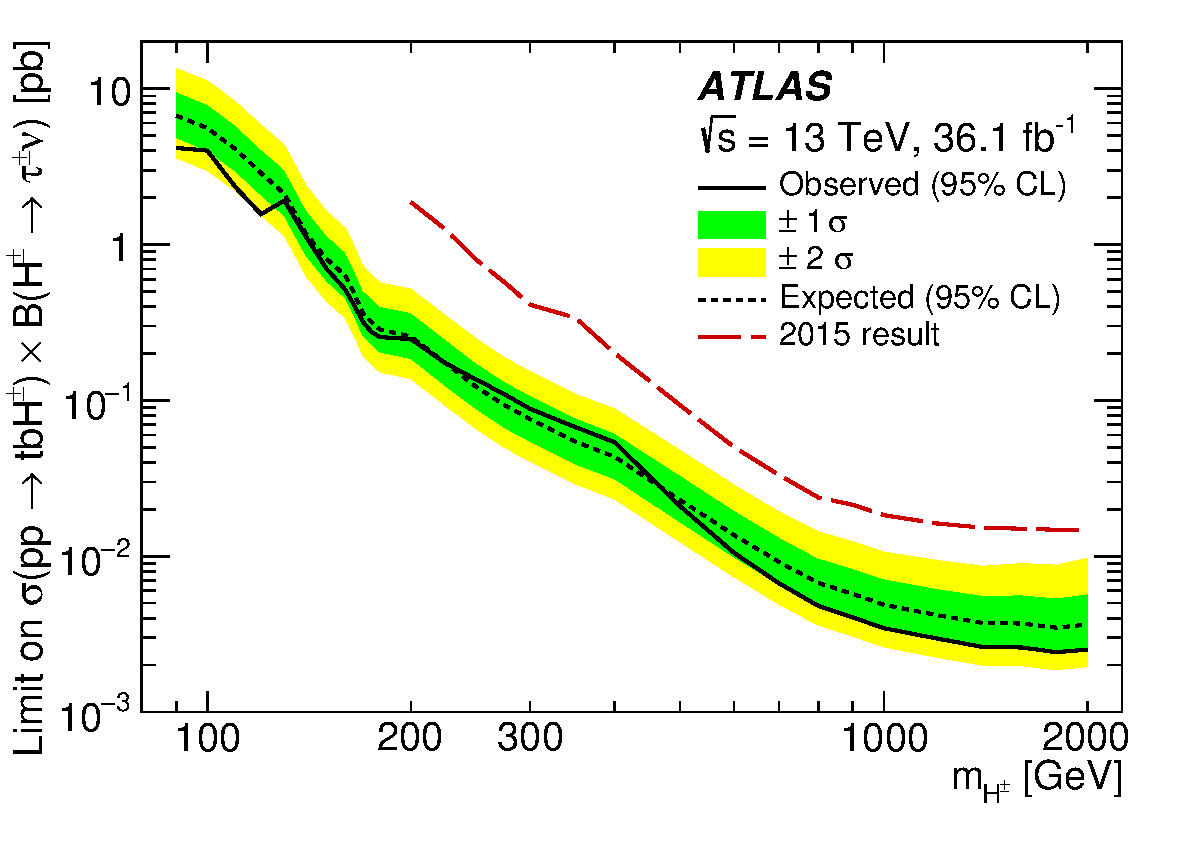
\includegraphics[width=0.40\linewidth]{Theory/Image/OldLimit/sigmaBR_atlas_13TeV_taunu.pdf}}
\vfil
\subfigure[Limit on \brThb \cite{Khachatryan:2015uua}]{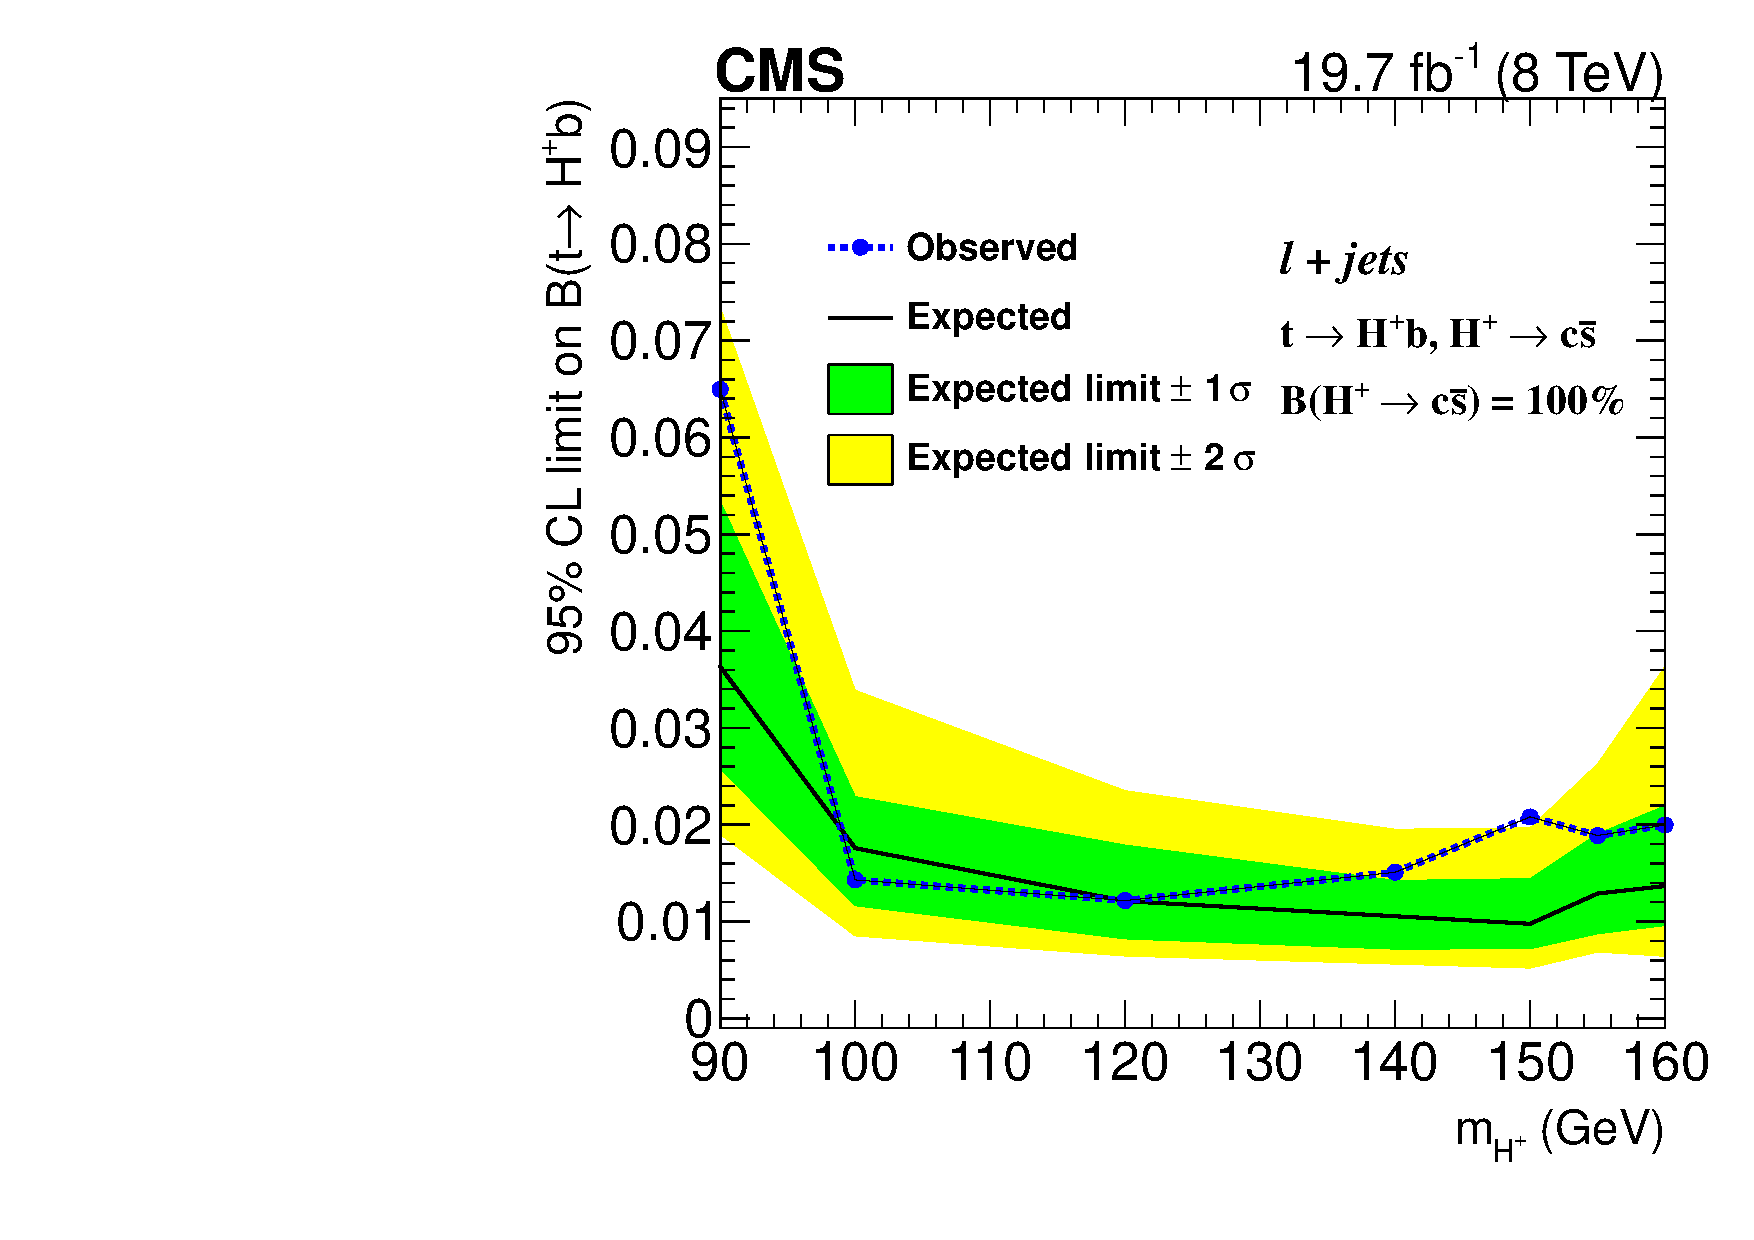
\includegraphics[width=0.45\linewidth]{Theory/Image/OldLimit/limit_CMS_csbar_8TeV.pdf}}
\subfigure[Limit on \sigHp$\times$\brHtv \cite{Sirunyan:2019hkq}]{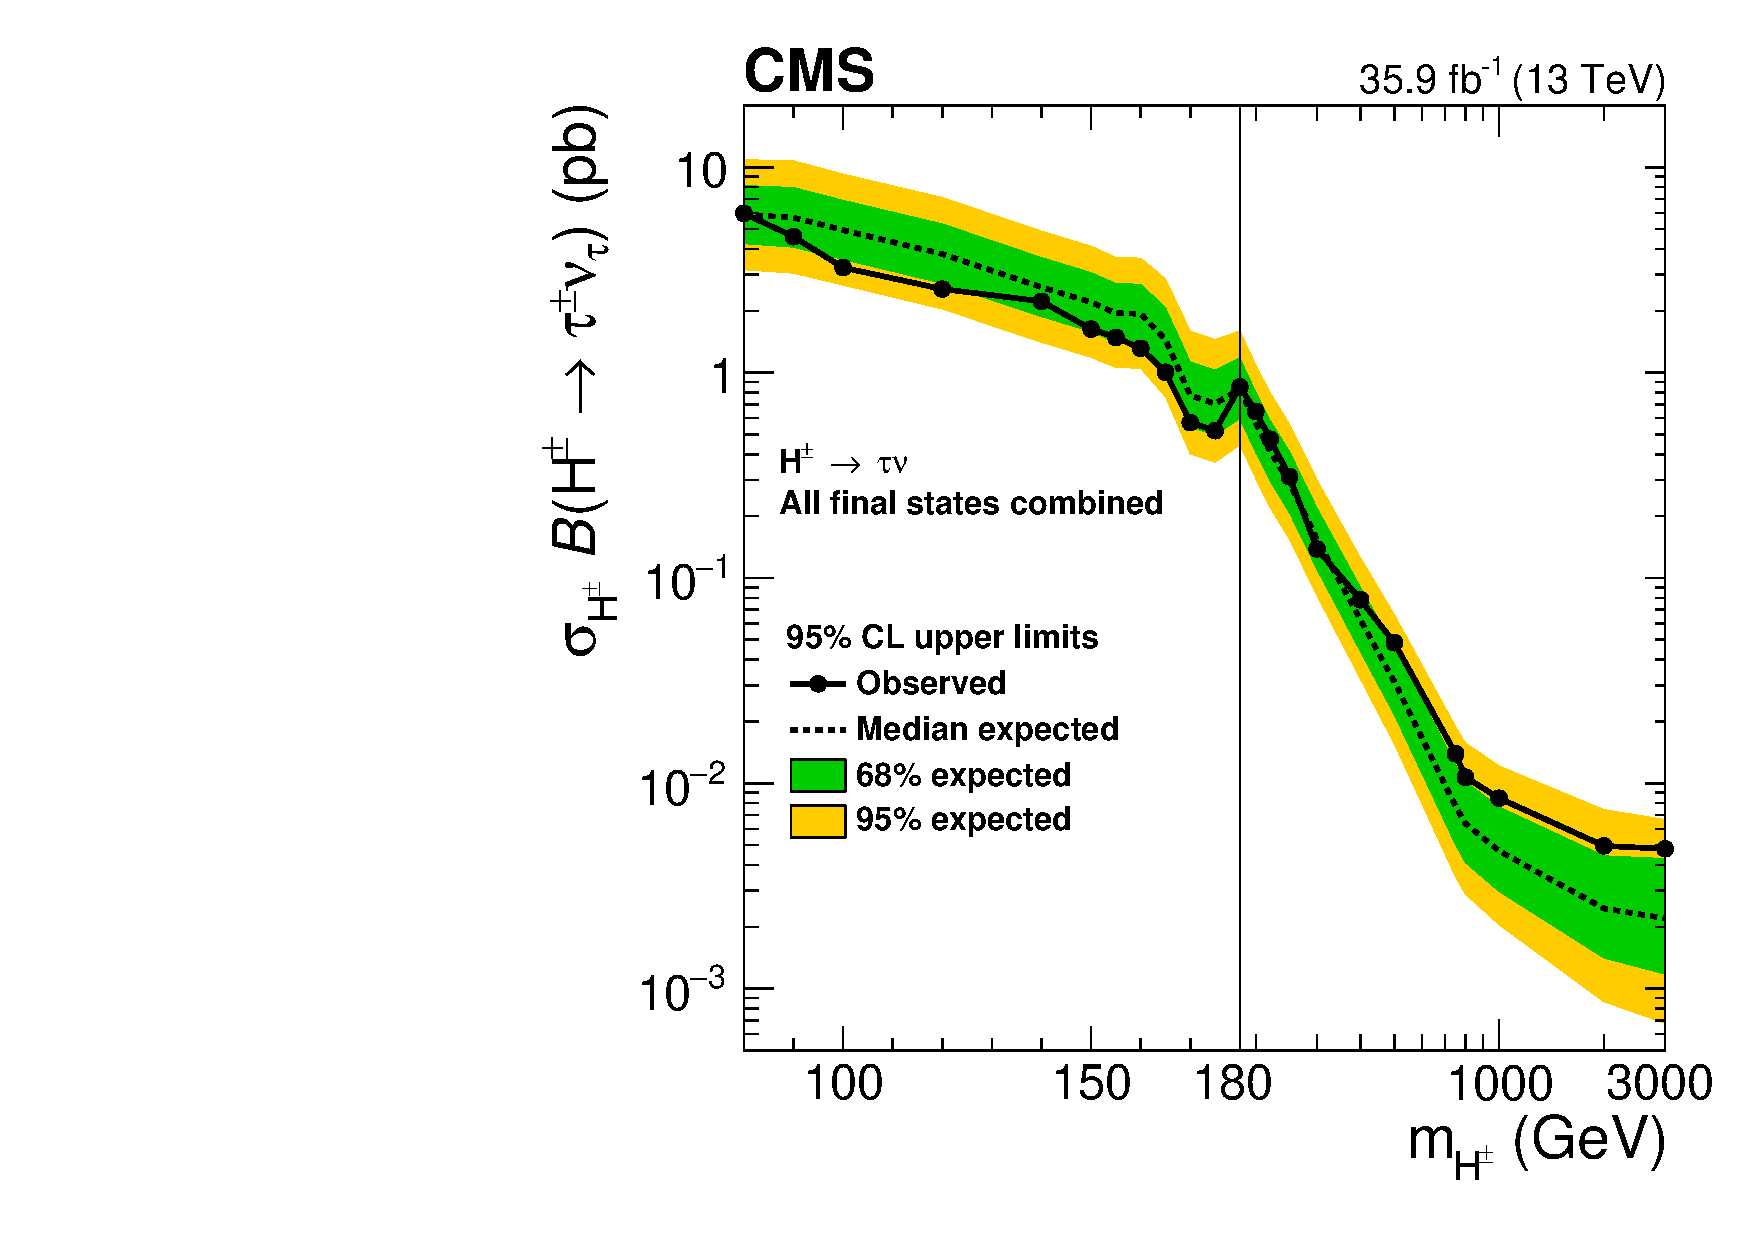
\includegraphics[width=0.45\linewidth]{Theory/Image/OldLimit/sigmaBR_cms_13TeV_taunu.pdf}}
\vfil
\subfigure[Limit in ($\tan\beta, ~\mHp$) plane \cite{Aaboud:2018gjj}]{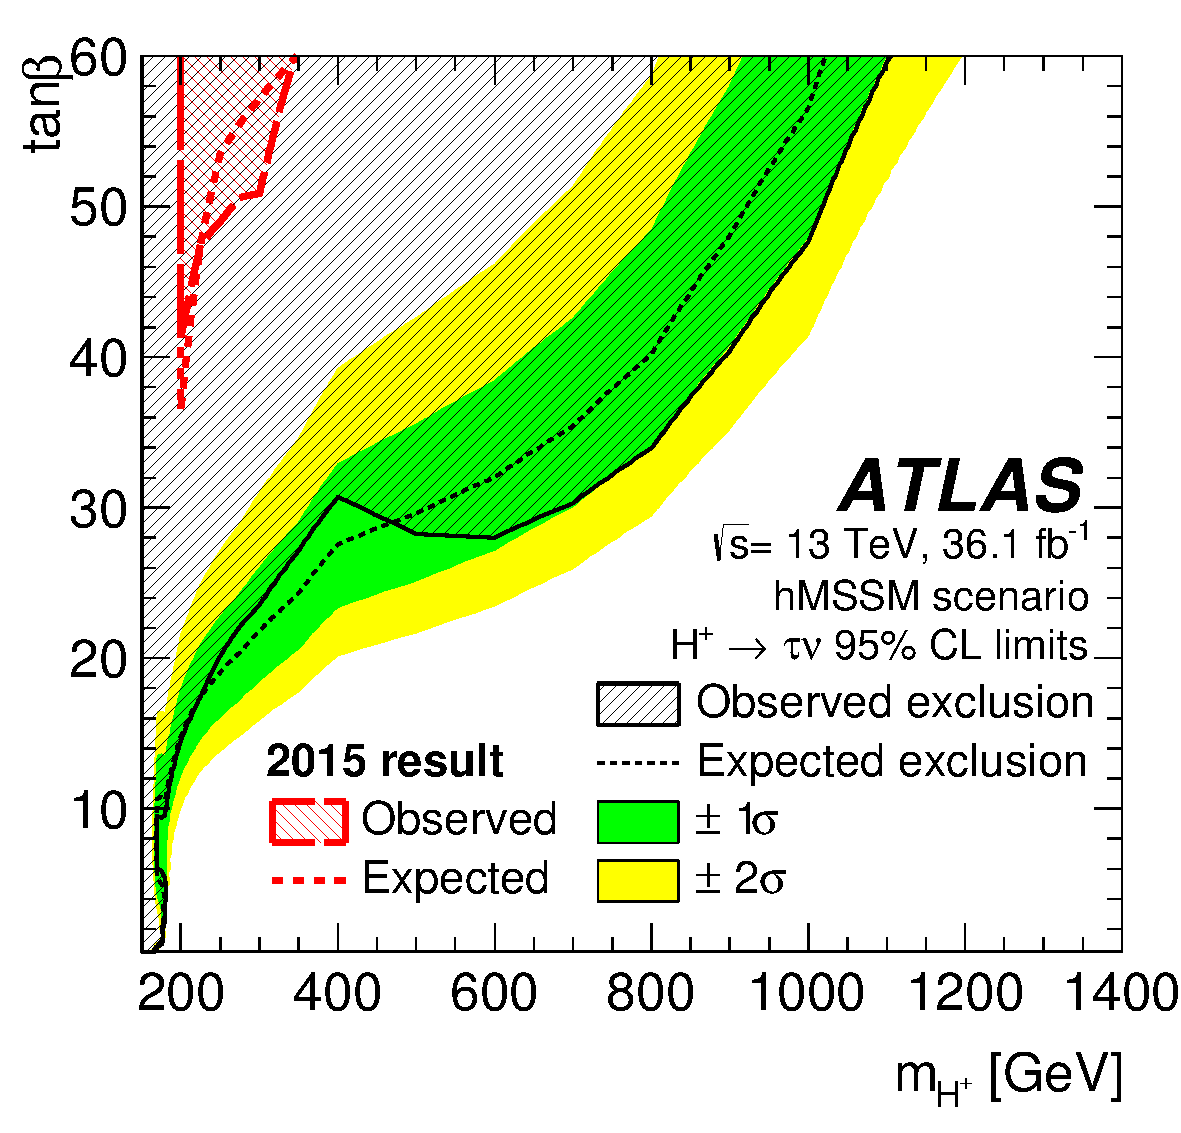
\includegraphics[width=0.45\linewidth]{Theory/Image/OldLimit/tanbeta_atlas_13TeV_taunu.pdf}}
\subfigure[Limit in ($\tan\beta, ~\mHp$) plane \cite{Sirunyan:2019hkq}]{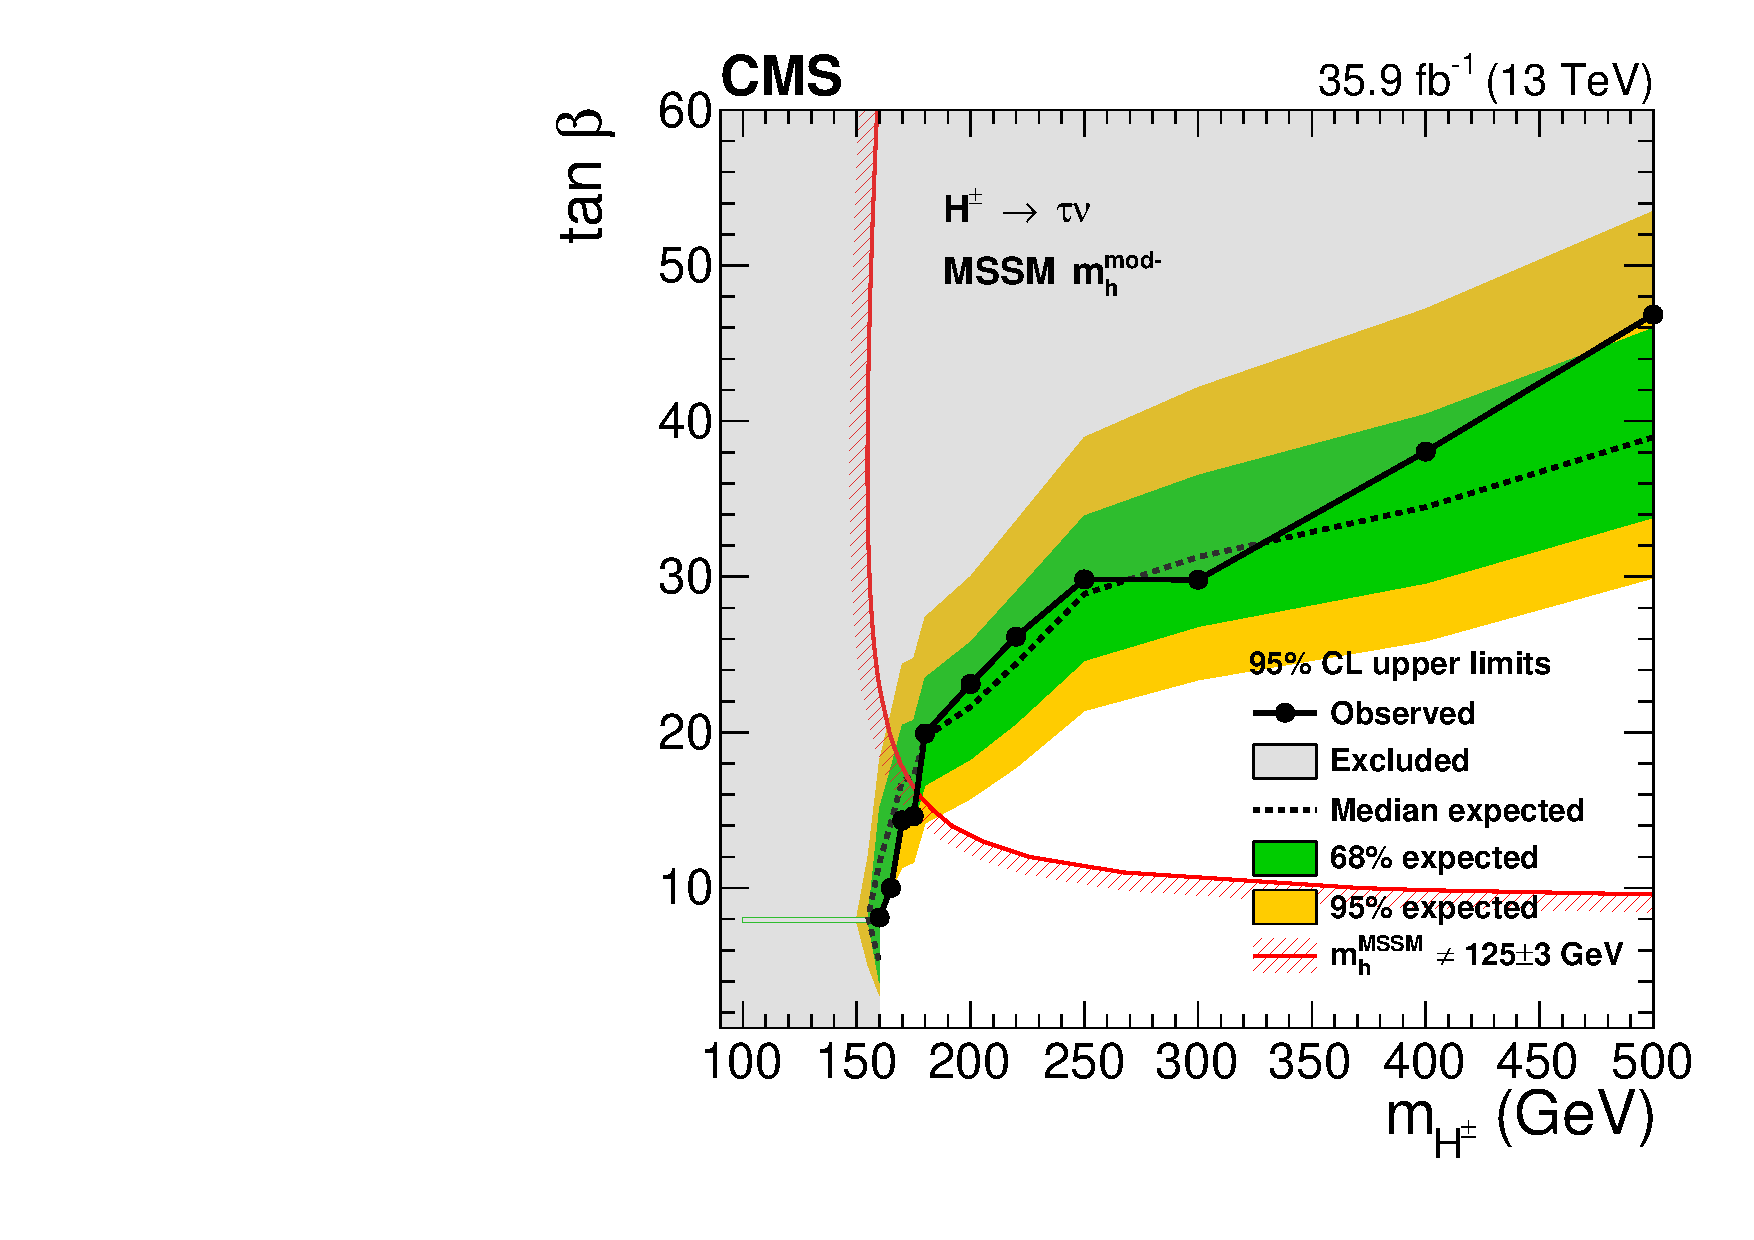
\includegraphics[width=0.45\linewidth]{Theory/Image/OldLimit/tanbeta_cms_13TeV_taunu.pdf}}
\caption{Current allowed range at 95\% CL from ATLAS and CMS.}
\label{fig:searchHplus}
\end{figure}




 
\section{Search strategy for the charged Higgs at 13 TeV}
\label{s:searchStrategy}

The search for the charged Higgs boson in the $c\bar{s}$ channel at 13 \TeV 
in the CMS experiment adopted a similar strategy as that of the previous analysis
at 8 \TeV \cite{Khachatryan:2015uua}. An additional charm quark tagging have been
further exploited to improve sensitivity. The invariant mass of the jets originating from 
charm and strange antiquark is taken as the observable for the search of charged Higgs, in the 
low mass region from 80 to 160 \GeV. In the absence of an excess in the observed data,
a 95\% CL limit is put on the \brThb. The charm tagging is extensively used to
improve this limit. As shown on the right side of the Figure~\ref{fig:feyn_diag_sig}, 
for the signal process, one \PQt quark decays to $H^+ b$ and the other one to 
$W^- \bar{b}$. The $W^+/H^+$ decays hadronically, whereas the $W^-$ decays 
leptonically. As a result, in the final states, there are four jets (2 \PQb jets, 
1 \PQc jet, 1 \PQs jet), one lepton (electron or muon, $\tau$ is not considered) 
and missing transverse energy attributed to neutrino. In this thesis, we assume that the \brHcs =100\%.
\begin{figure}
\centering
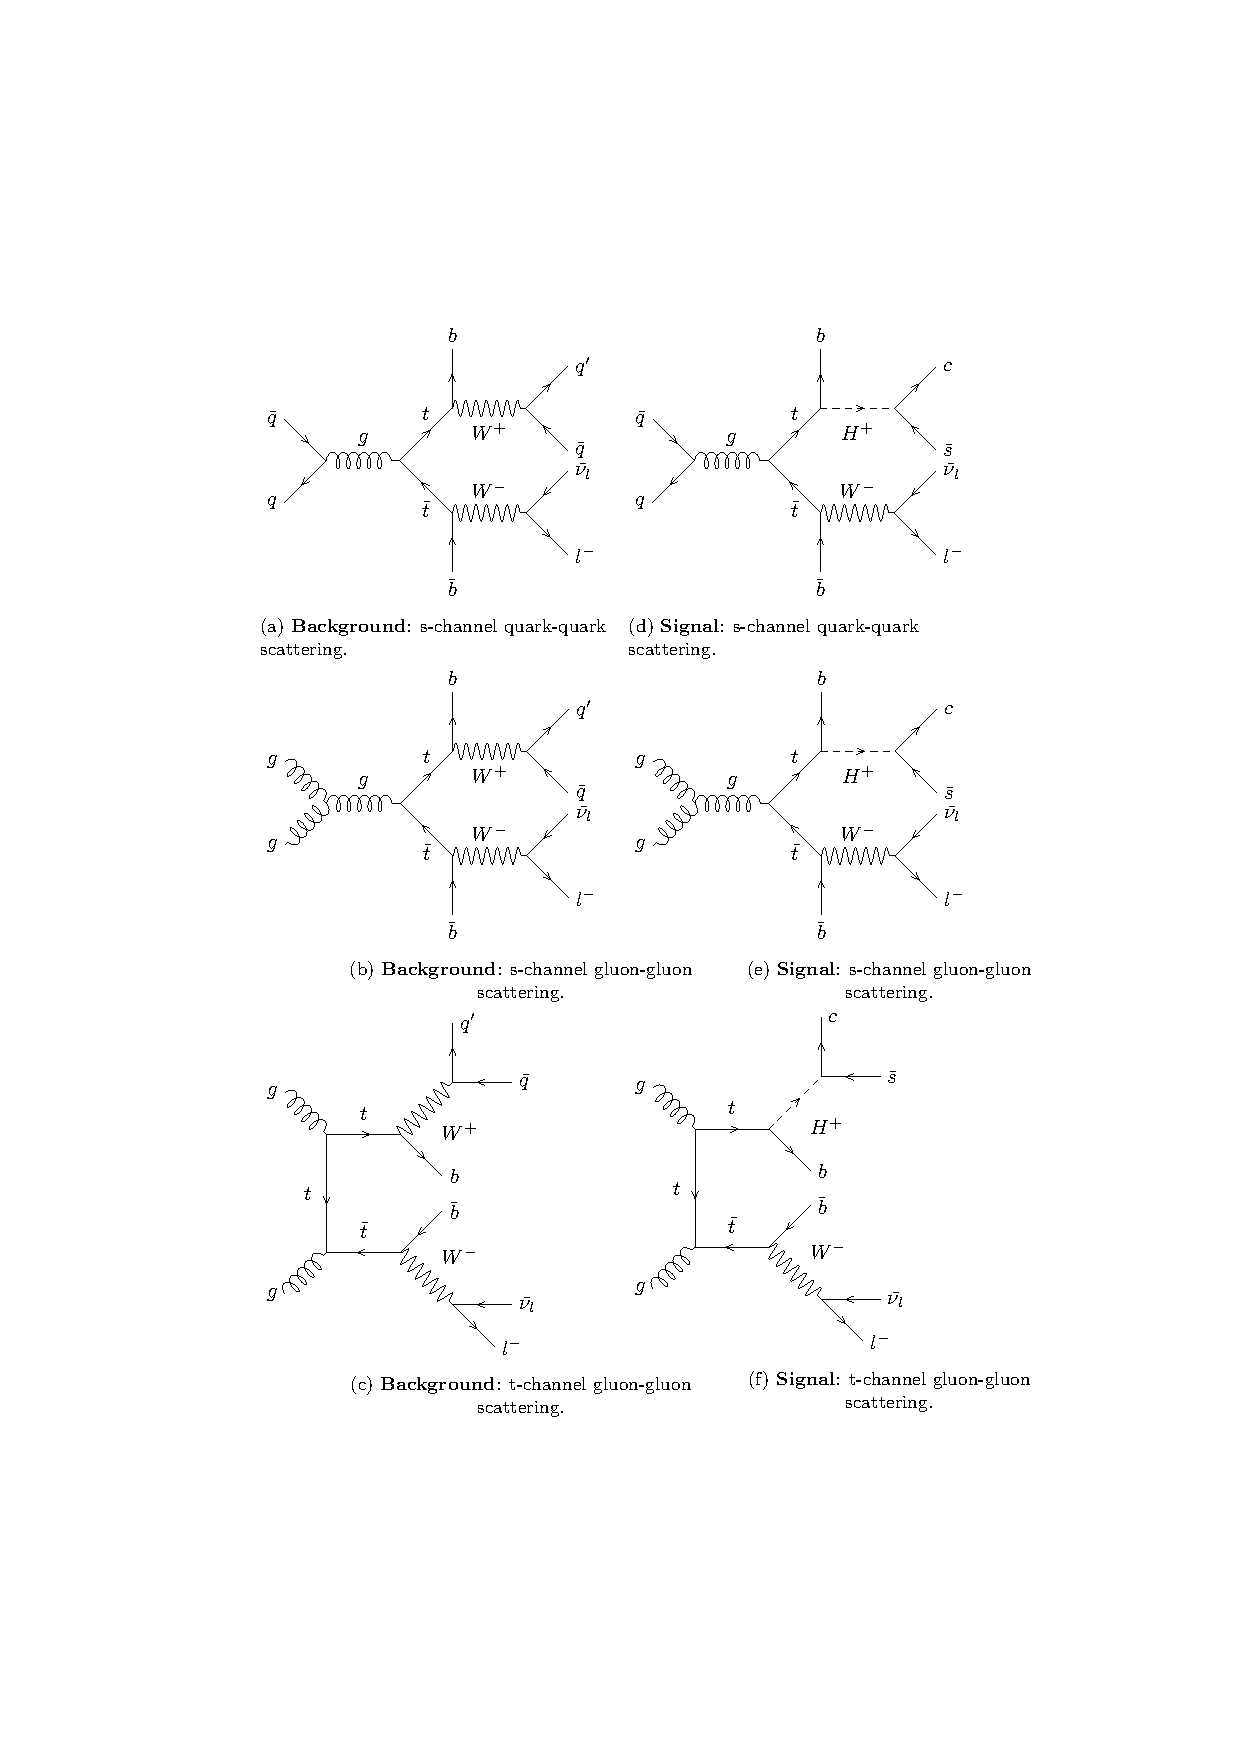
\includegraphics[width=0.75\textwidth]{Image/FeynDiag/feyn_diag_sig.pdf}
\caption{Production of \ttbar from gluon-gluon and quark-quark scattering. 
         The quark-scattering production process has a dominant contribution at 
         Tevatron energies whereas gluon-gluon scattering diagrams are dominant 
         at LHC energies ~\cite{Gerber:2014xea, Fiorini:2012fe}. The SM production
         of \ttbar is shown in (a), (b) and (c). The charged Higgs boson 
         production and its decay are shown in (d), (e), and (f).}
\label{fig:feyn_diag_sig}
\end{figure}

The standard Model processes that give same final states (4 jets + 1 lepton + missing 
energy) are considered as backgrounds for this analysis. The standard model
\ttbar production is the most dominant, irreducible background process. 
As shown in the left side of the Figure~\ref{fig:feyn_diag_sig}, for
SM \ttbar process, one \PQt quark decays to the $W^+$ and \PQb quark 
($t\rightarrow W^+ b$) and the other decays to $W^- \bar{b}$ 
($\bar{t}\rightarrow W^-\bar{b}$). The SM \ttbar contributes around 94\%
of the total backgrounds. Other sub-dominant backgrounds that give rise to similar 
final states are single \PQt quark production, QCD multijet, \wjets, \dyjets, 
and vector boson pair production processes. The following background processes are considered
for the search for charged Higgs. They are ordered in their significance of contribution.
\begin{enumerate}[leftmargin=*]
\item $\textbf{SM \ttjets}$: Feynman diagrams 
	for \ttjets production are shown on the left hand side of Figure
	\ref{fig:feyn_diag_sig}. This is the most dominant background channel
	in the signal search region (SR).

\item {\bf{Single \PQt}}: The single \PQt quark production process can also mimic the signal 
	topology. Three different ways, as shown in Figure~\ref{fig:feyn_diag_st}, 
	of production of single top quark considered in this analysis. It is produced through 
	s-channel, t-channel, and tW-channel. In the s-channel and t-channel the initial quarks 
	can be \PQu, \PQd, \PQc and \PQs (4-flavour scheme). However, in the tW-channel, 
	the initial quark is only \PQb quark (5-flavor scheme).
	\begin{figure}
	\begin{center}
	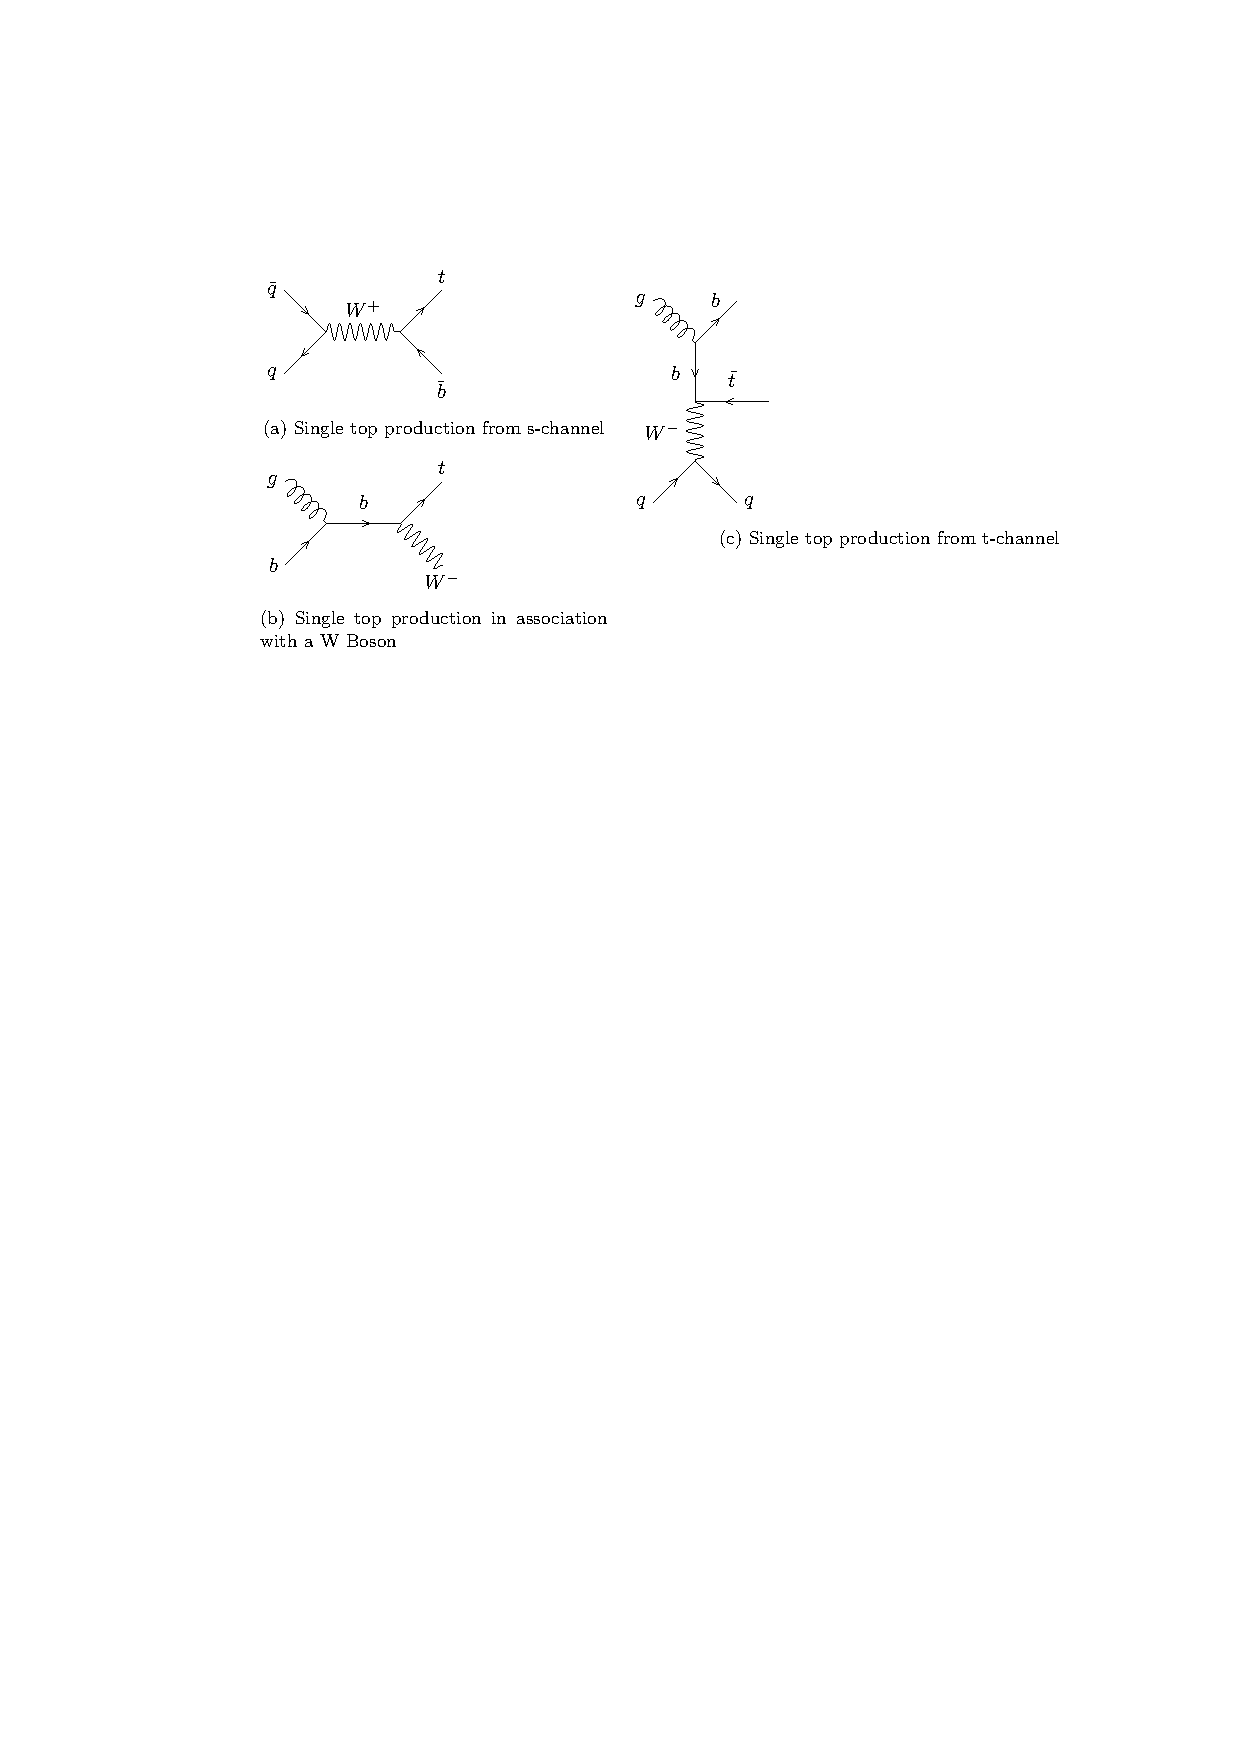
\includegraphics[width=0.75\textwidth]{Image/FeynDiag/feyn_diag_st.pdf}
	\caption{Representative Feynman diagrams for single \PQt quark production processes.}
	\label{fig:feyn_diag_st}
	\end{center}
	\end{figure}

\item {\bf{QCD multijet}}: The QCD multijet events contain only jets at parton level. However, after
	event reconstruction, they can still have leptons from misidentifications, and \MET due to 
	poor measurement of energy in the detector. Thus these events also mimic the signal topology.

\item {\bf{\wjets}}: In this process, a \PW boson is produced in the proton-proton 
	collisions which subsequently decays leptonically. Following \wjets 
	background process are considered in this analysis:
  	\begin{enumerate}[leftmargin=*]
  	  \item $\PW + \rm{jets  }(\PW^\pm \rightarrow l^+ \nu (l^-\bar{\nu}))$
  	  \item $\PW + \rm{1 jet }(\PW^\pm \rightarrow l^+ \nu (l^-\bar{\nu}))$
  	  \item $\PW + \rm{2 jets }(\PW^\pm \rightarrow l^+ \nu (l^-\bar{\nu}))$
  	  \item $\PW + \rm{3 jets }(\PW^\pm \rightarrow l^+ \nu (l^-\bar{\nu}))$
  	  \item $\PW + \rm{4 jets }(\PW^\pm \rightarrow l^+ \nu (l^-\bar{\nu}))$
  	\end{enumerate} 
	The Feynman diagram for these processes are shown in Figure~\ref{fig:feyn_diag_wjet}.
	\begin{figure}
	\begin{center}
	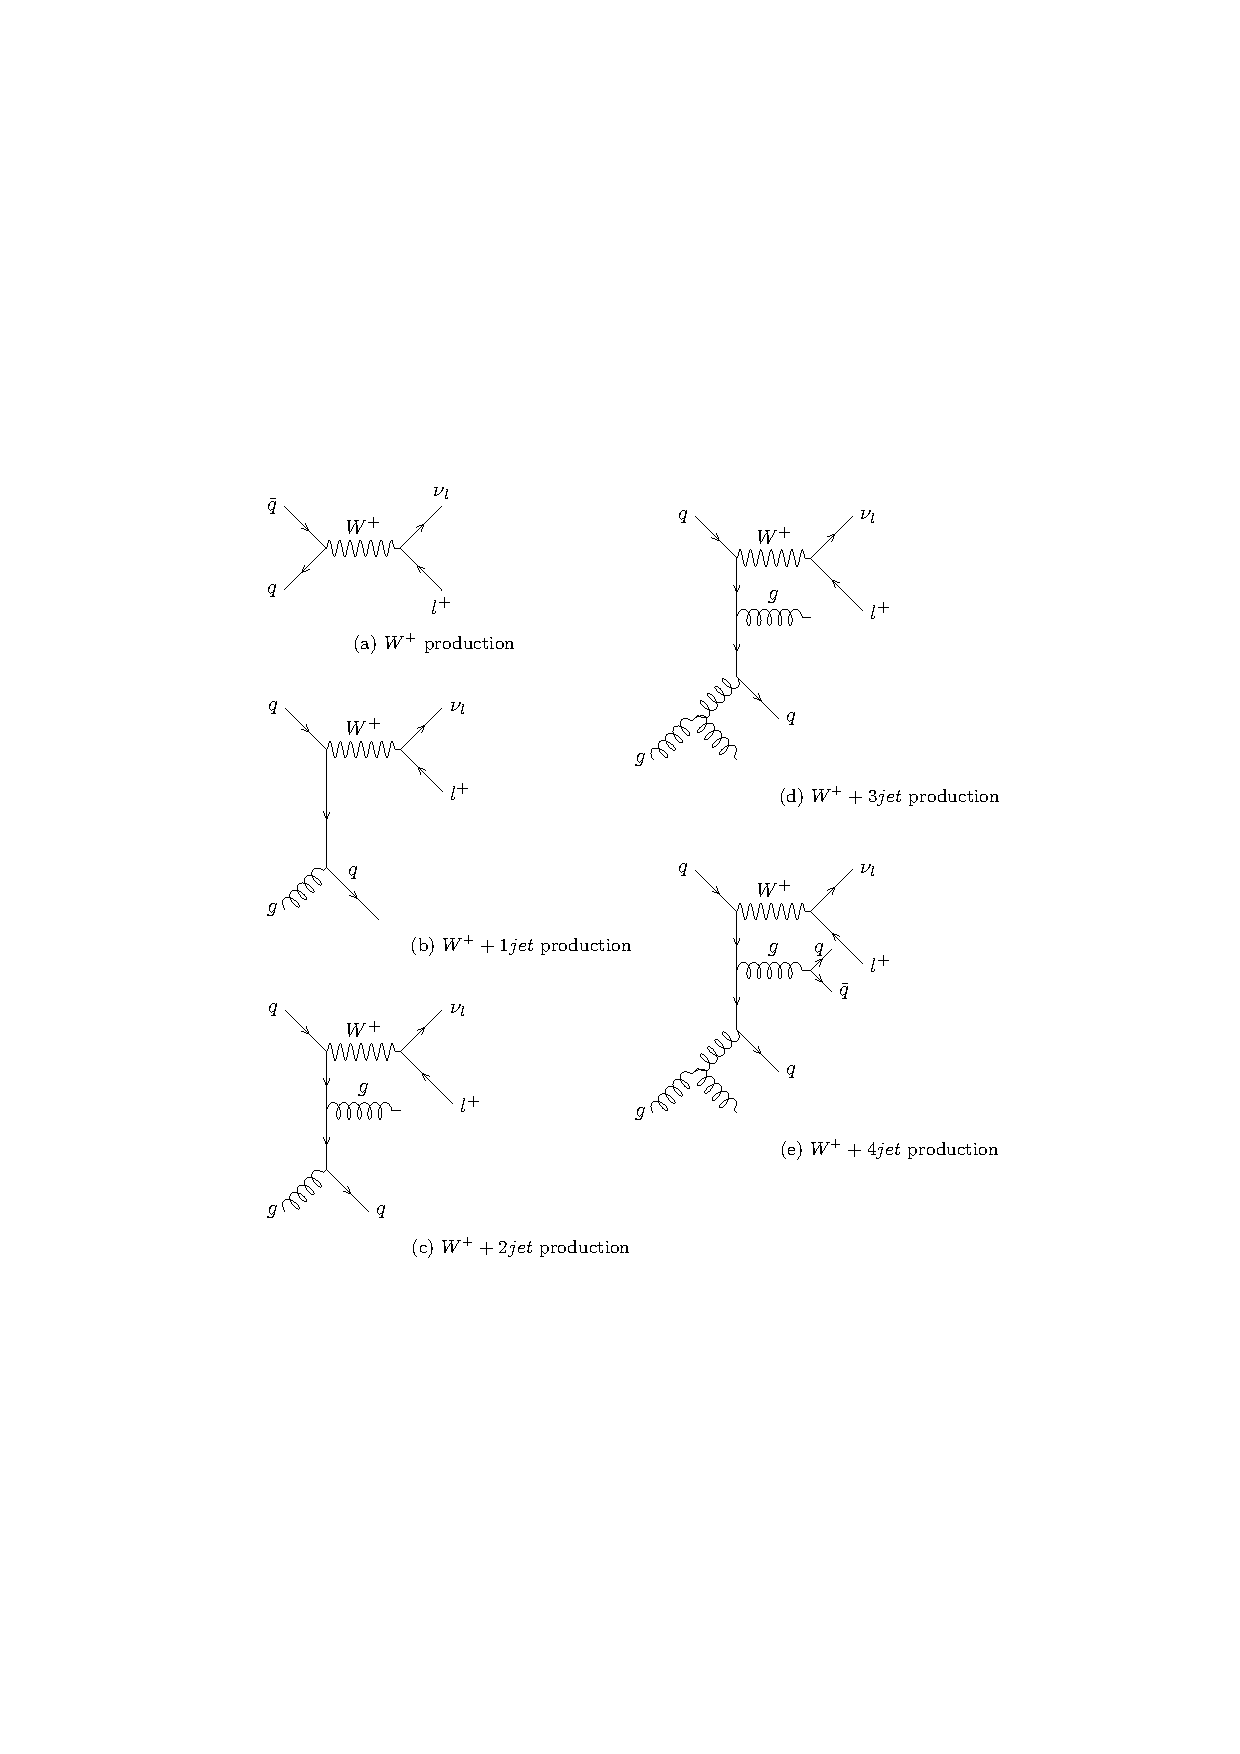
\includegraphics[width=0.75\textwidth]{Image/FeynDiag/feyn_diag_wjet.pdf}
	\caption{Representative Feynman diagrams for $\PW + \rm{n jets}$ channel. The 
	\PW boson is produced by quark-quark and quark-gluon scattering 
	along with n jets (n = 0, 1, 2, 3, 4).}
	\label{fig:feyn_diag_wjet}
	\end{center}
	\end{figure}

\item ${\bf{Z/}}$$\gamma$ ${\bf{+ jets}}$: The Drell-Yan processes in which 
	$Z/\gamma$ are produced along with jets, have lepton and jets at parton level as 
	shown in Figure~\ref{fig:feyn_diag_dyjet}. However, after the 
	reconstruction, the \MET is also found in the events due to the poor 
	measurement of energy in the detector.
	\begin{enumerate}[leftmargin=*]
  	\item $Z/\gamma +\rm{ jets   }(Z/\gamma \rightarrow l^+ l^-)$
  	\item $Z/\gamma +\rm{ 1 jet  }(Z/\gamma \rightarrow l^+ l^-)$
  	\item $Z/\gamma +\rm{ 2 jets }(Z/\gamma \rightarrow l^+ l^-)$
  	\item $Z/\gamma +\rm{ 3 jets }(Z/\gamma \rightarrow l^+ l^-)$
  	\item $Z/\gamma +\rm{ 4 jets }(Z/\gamma \rightarrow l^+ l^-)$
  	\end{enumerate}
	\begin{figure}
	\begin{center}
	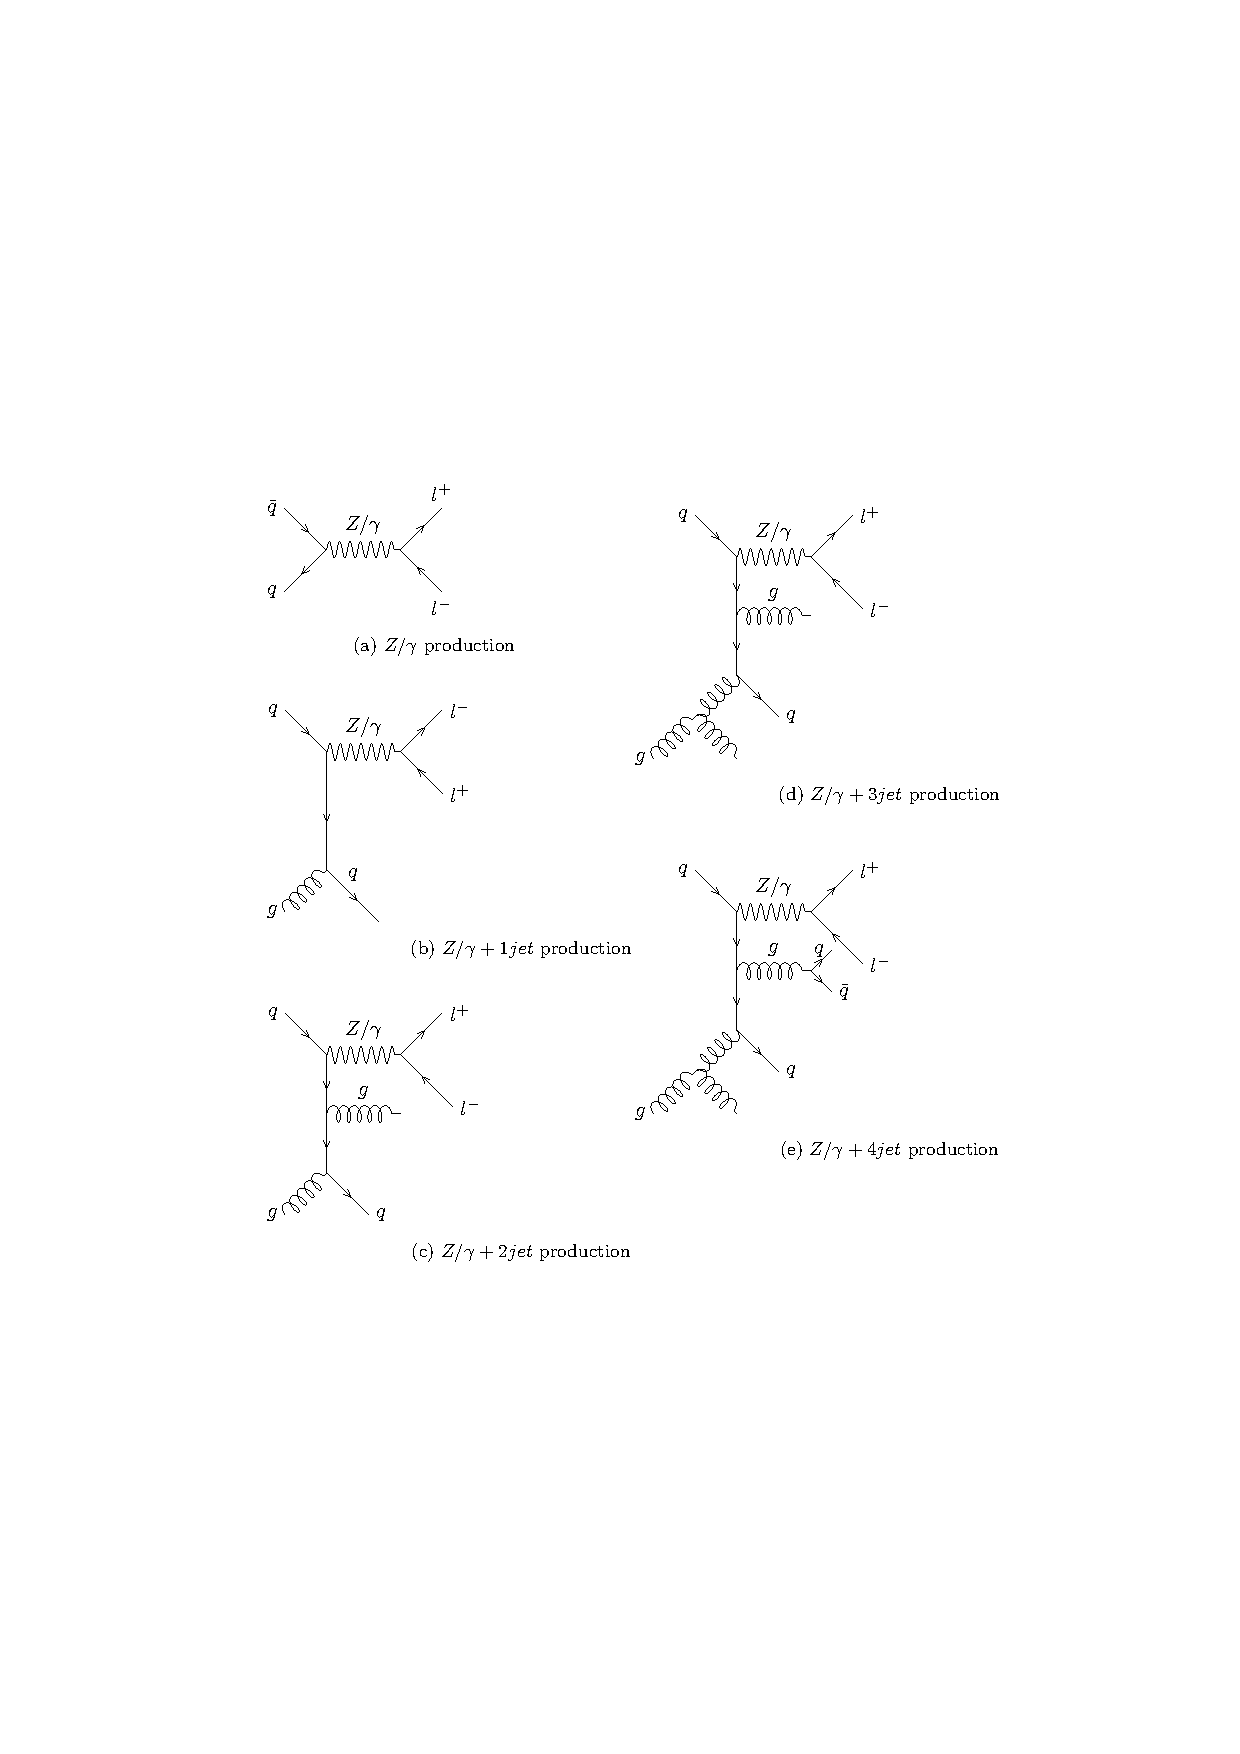
\includegraphics[width=0.75\textwidth]{Image/FeynDiag/feyn_diag_dyjet.pdf}
	\caption{Representative Feynman diagrams for $ Z/\gamma + \rm{n jets}$ channel. 
	The $Z/\gamma$ is produced by quark-quark and quark-gluon scattering 
	along with n jets (n = 0, 1, 2, 3, 4).}
	\label{fig:feyn_diag_dyjet}
	\end{center}
	\end{figure}

\item {\bf{VV}}: Vector boson fusion processes are the smallest background in the signal 
	search region. The fusion happens via tri-linear coupling between the 
	$W^\pm$ and \PZ. The \PZ boson further decays to $l^+l^-$. The vector boson pair production process (VV) has 
	three sub-categories: WW, WZ, and ZZ.
\end{enumerate}




\part{The CMS Experiment at The LHC, CERN}
\label{part:cms} 
\chapter{The LHC at CERN}
\label{c:lhc}
\section{Introduction}
\label{s:secIntroLHC}
The European Organisation for Nuclear Research 
(CERN- \emph{Conseil Europ\'{e}n pour la Recherche Nucl\'{e}aire}), located at Geneva, 
Switzerland, is one of the leading laboratories in the world in the field of experimental 
high energy physics. The experimental collaborations at CERN involve more than 1700 people 
from 41 countries. The research activity at CERN ranges from the understanding of fundamental 
constituents of matter such as the Higgs Boson to the hunt of dark matter. Particles such as protons 
(p), lead nuclei (Pb) are accelerated to a very high speed (nearly the speed of light) and collided 
head-on. The acceleration of these particles proceeds in several stages, such as shown in Figure 
\ref{fig:lhc}.
\begin{figure}
  \begin{center}
  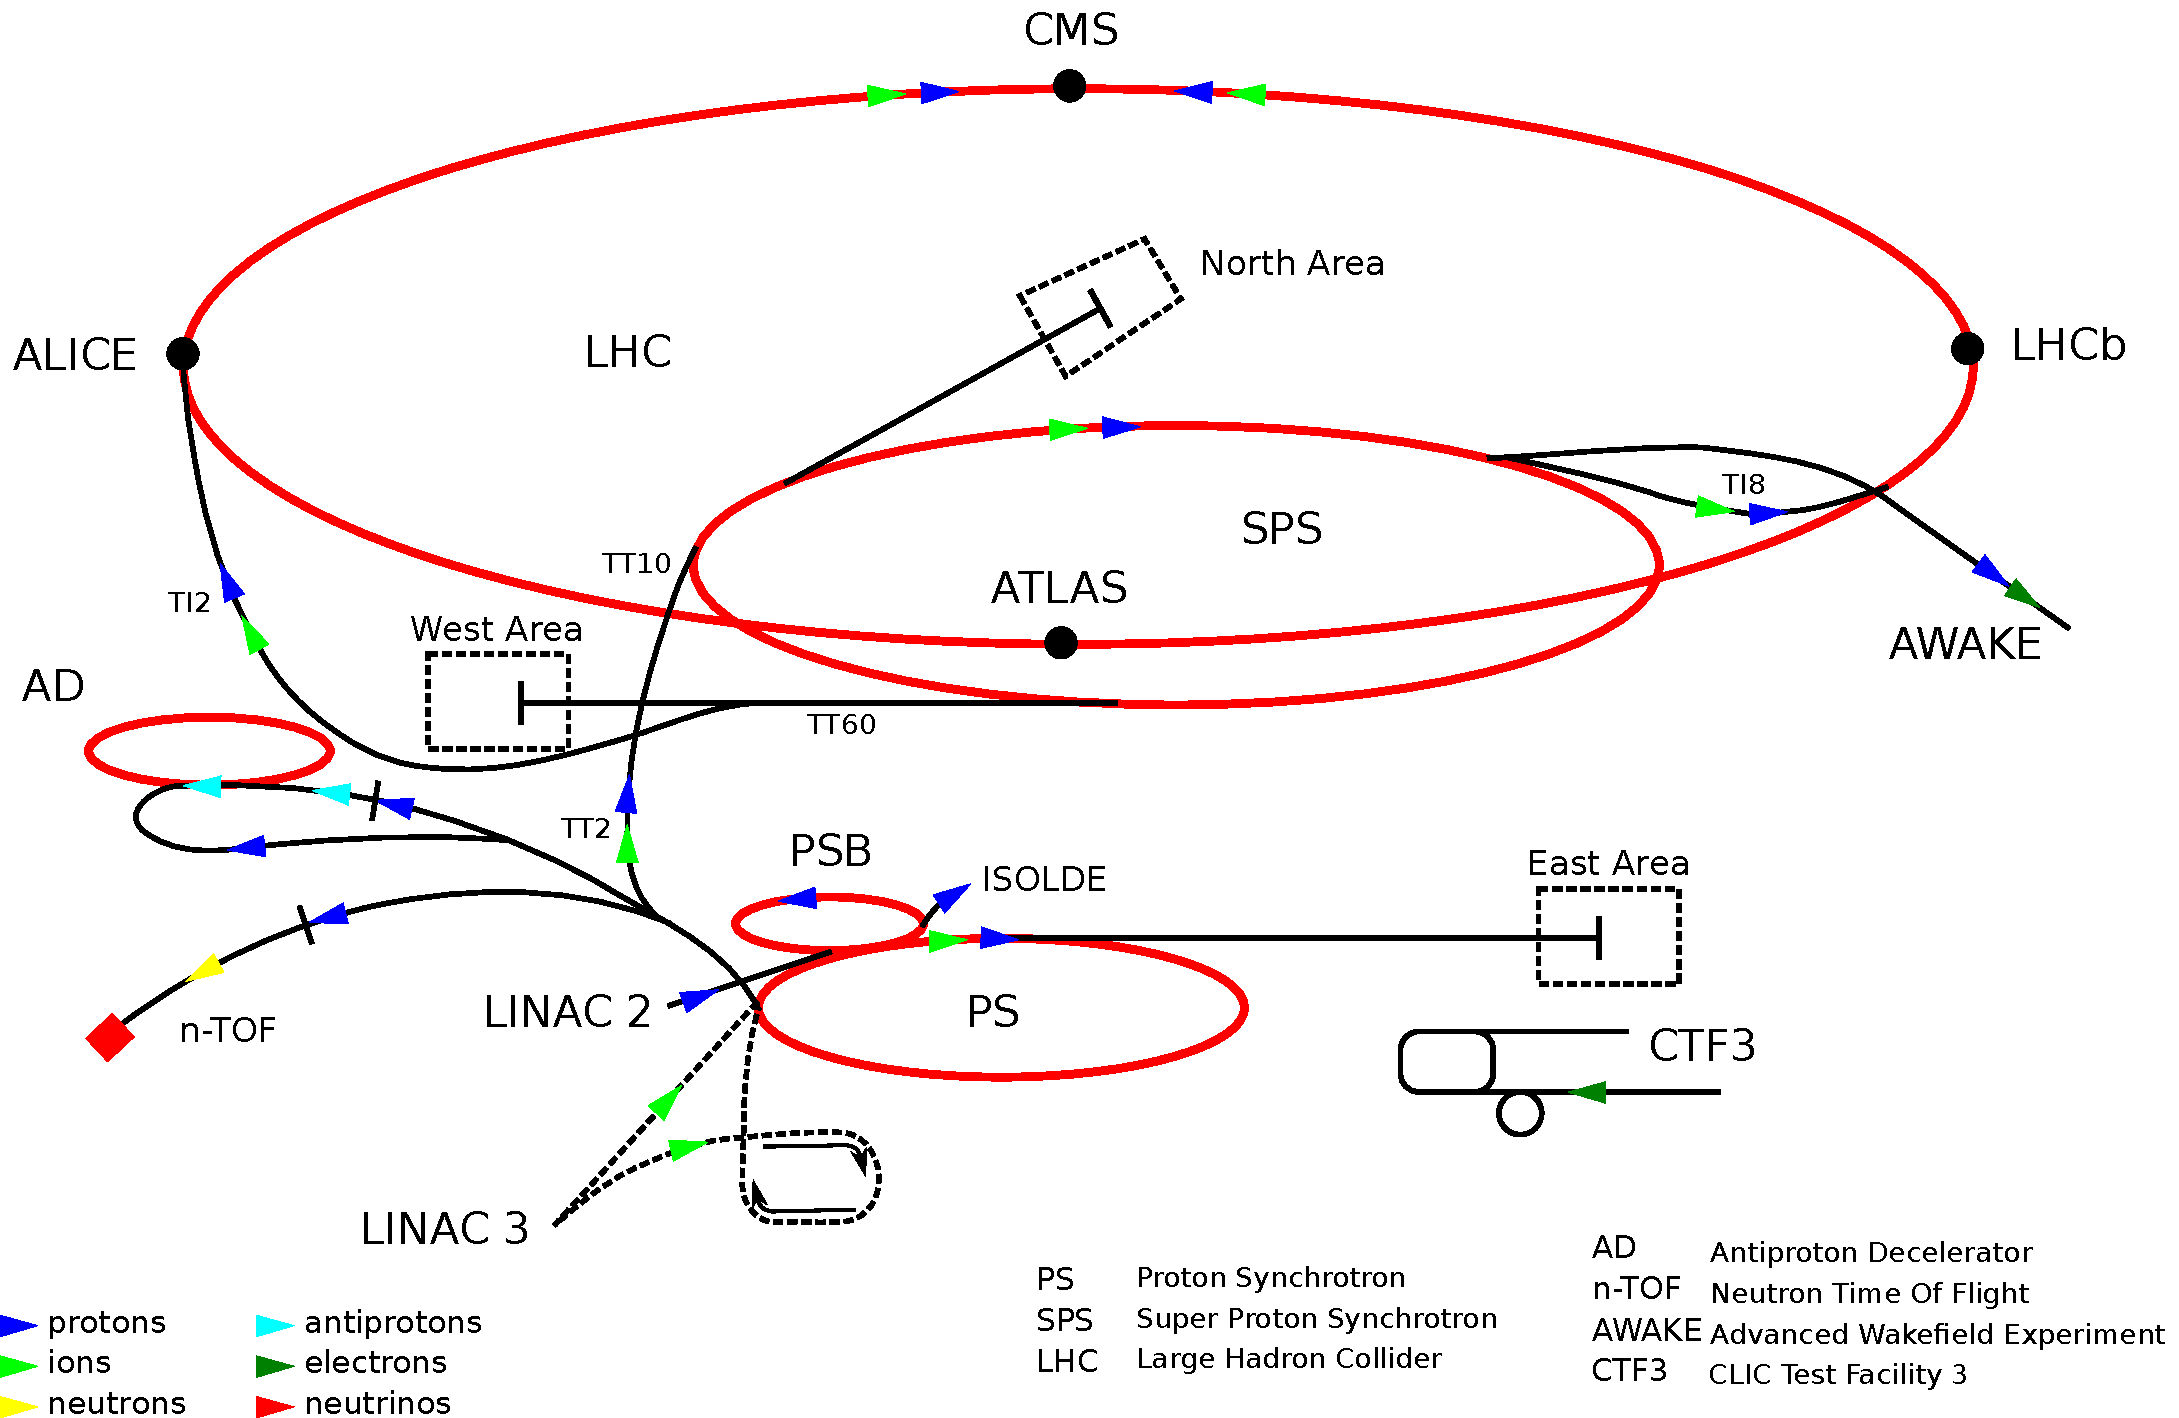
\includegraphics[width=0.80\linewidth]{Experiment/LHC/Image/cernacc.pdf}
  \caption{The CERN accelerator complex~\cite{wiki:cernAcc}. The particles are accelerated 
	at various stages, starting from LINAC to PSB to PS to SPS to LHC. Various detectors 
	such as ATLAS, LHCb, CMS, and ALICE are placed at the collision points.}
  \label{fig:lhc}
  \end{center}
\end{figure}

Bunches of protons (\emph{$H^+$}, after the electron is stripped-off from a hydrogen 
atom) are first passed through the Linear Accelerator (LINAC2), which accelerates the 
protons to an energy of 50 \MeV. Subsequently, the proton bunches are passed through the 
Proton Synchrotron Booster (PSB) which accelerates the protons to an energy of 1.4 \GeV.
Further, the bunches are circulated in a bigger Proton Synchrotron (PS) accelerating protons 
up to an energy of 26 \GeV. After that, the proton bunches are circulated 
inside the Super Proton Synchrotron (SPS) which accelerates them to an energy of 
450 \GeV. Finally, the bunches are injected into the Large Hadron Collider (LHC)
ring. Where protons are accelerated to a speed of 99.99\% of the speed of light.
At such a large speed the proton bunches come so close that they look like a beam. 
The increment in the energy of protons at various stages are listed in 
Table~\ref{tab:lhc}.
\begin{table} 
\caption{\label{tab:lhc} The energy of protons after passing through various 
	accelerators.} 
\begin{centering} 
\begin{tabular}{cc} 
\hline  
\hline 
\noalign{\vskip 0.1cm}
LINAC2 & 50 \MeV \tabularnewline 
\noalign{\vskip 0.1cm}
PSB & 1.4 \GeV \tabularnewline 
\noalign{\vskip 0.1cm}
PS & 26 \GeV \tabularnewline 
\noalign{\vskip 0.1cm}
SPS & 450 \GeV \tabularnewline 
\noalign{\vskip 0.1cm}
LHC & 7 \TeV \tabularnewline 
\hline  
\hline 
\end{tabular} 
\par\end{centering} 
\end{table}

A typical synchrotron consists of many components such as dipole magnets to bend the beams,
quadrupole magnets to focus the beams, radio frequency (RF) cavities to accelerate
the beams, cryogenics for superconducting and cooling the LHC ring, and beam diagnostics
to monitor the beam movement.
Two proton beams, moving in the opposite direction, are collided at four points of 
the LHC ring, as shown in Figure~\ref{fig:lhcRing}. 
\begin{figure}
  \begin{center}
  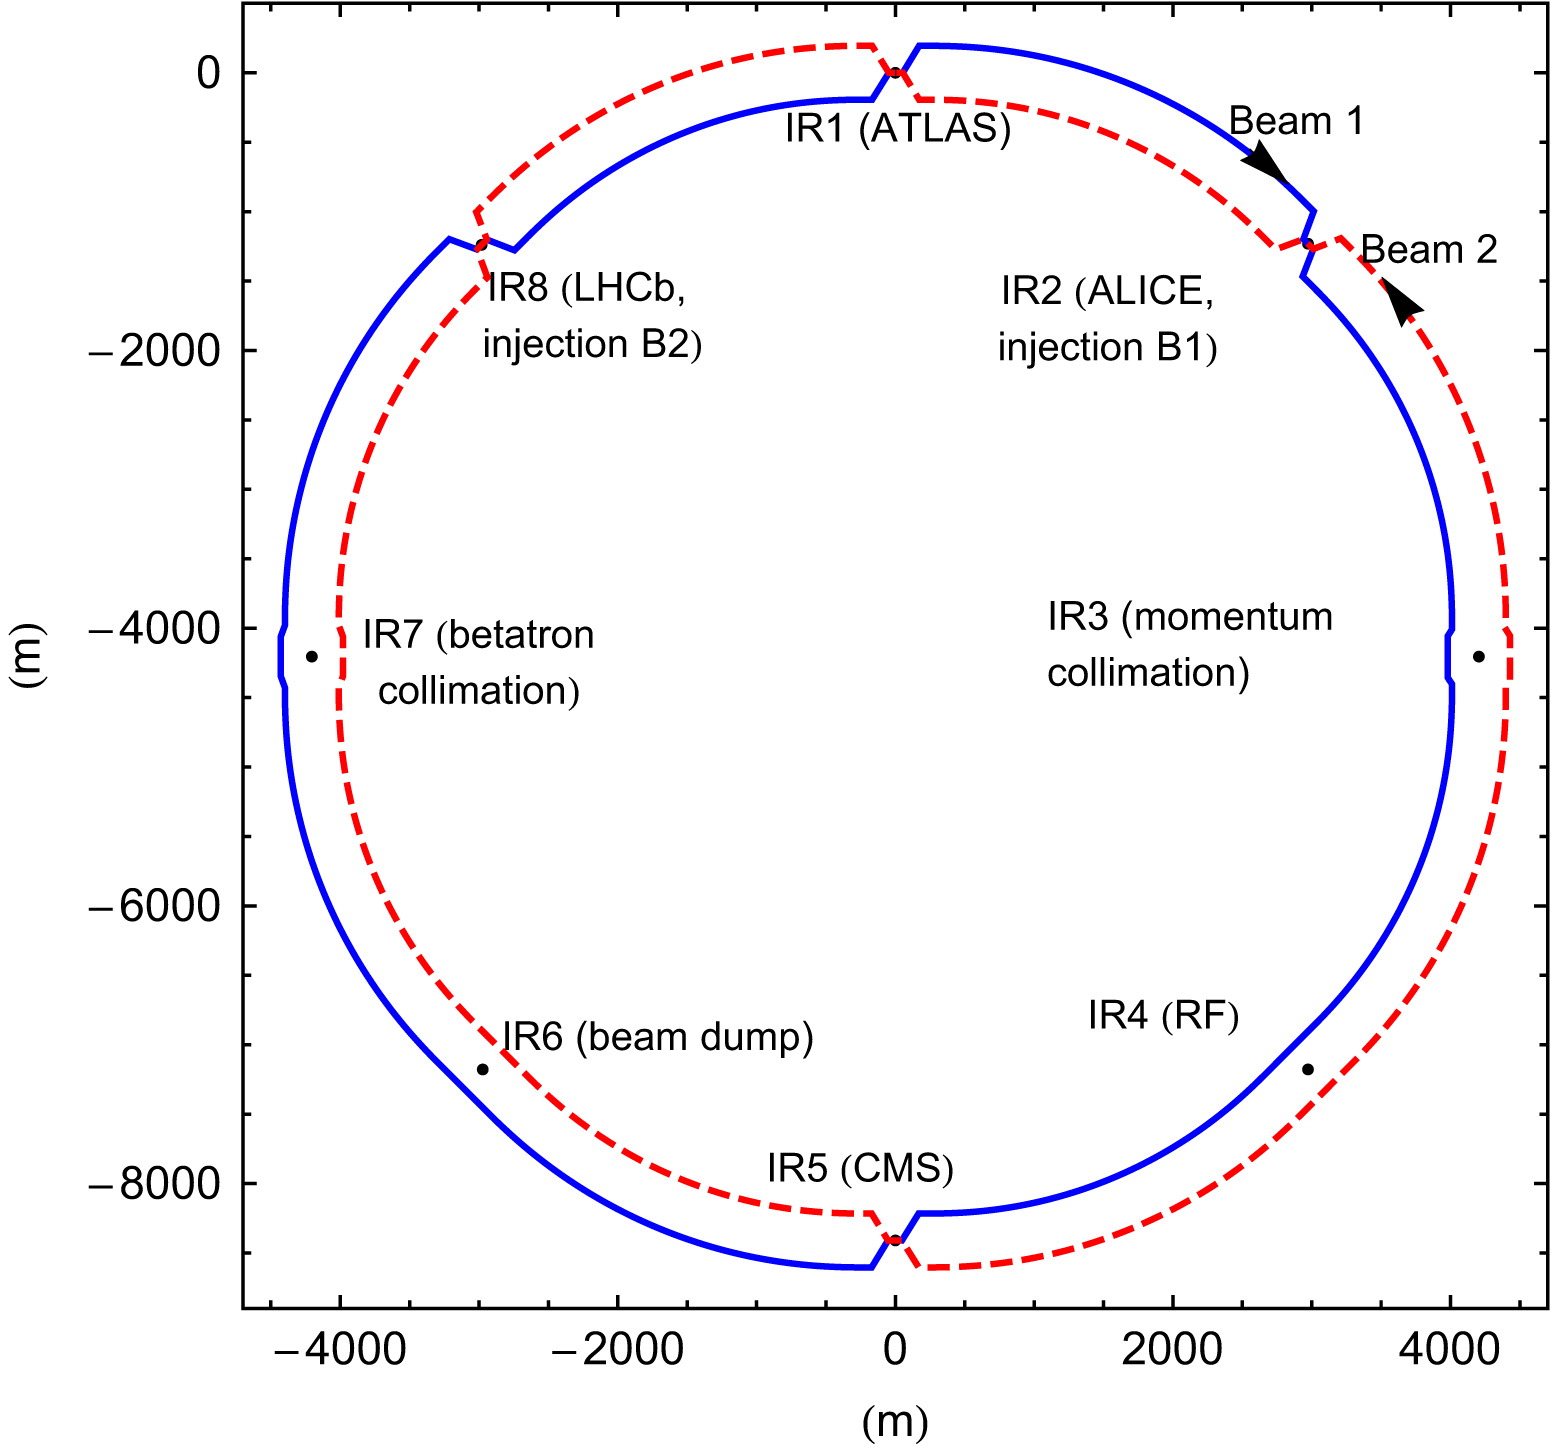
\includegraphics[width=0.50\linewidth]{Experiment/LHC/Image/lhc_ring.jpg}
	  \caption{The layout of insertion regions (IRs) at the LHC ring \cite{BRUCE2013825}.
	  The separation between the two colliding beams is not to scale. The 
	  separation between them is exaggerated for illustration. The total circumference
	  of the LHC ring is 27\unit{km}. Oppositely moving beams (Beam 1 and 2) are made 
	  to collide at four points of the ring. At the collision points, detectors such as
	  CMS, ALICE, ATLAS, and LHCb are installed to record the collision.}
  \label{fig:lhcRing}
  \end{center}
\end{figure}

There are eight insertion regions (IRs) at the LHC ring as shown in Figure~\ref{fig:lhcRing}. 
At four of them, where collision happens, four main detectors are installed,
ATLAS at IR1, ALICE at IR2, CMS at IR5, and LHCb at IR8. Three other small detectors namely 
LHCf, TOTEM, and MoEDAL are placed in the same cavern as ATLAS, CMS, and LHCb, 
respectively. At other IRs, the collimators are installed 
such as the momentum collimator at IR3, betatron at IR7, and RF at IR4. The beam dumping system 
is placed at IR6. Near the collision points, various systems such as dipole and quadrupole
magnets are installed to bend and focus the proton beams as shown in Figure~\ref{fig:lhc_beamBend}.
Using these magnets the two counter rotating beams are brought closer for a head-on
collision. A brief description of various detectors is given in the next section.
%https://cds.cern.ch/record/2207171/plots
\begin{figure}
  \begin{center}
  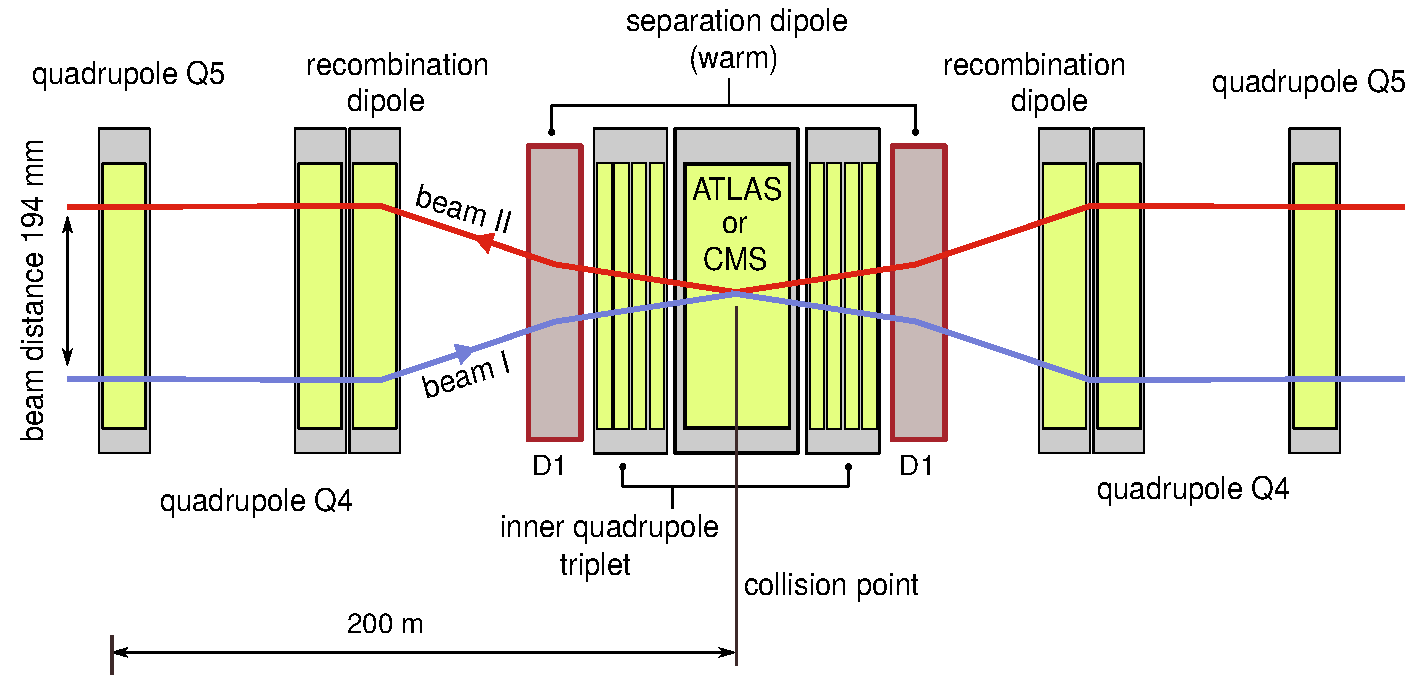
\includegraphics[width=0.75\linewidth]{Experiment/LHC/Image/lhc_beamBend.pdf}
  \caption{Schematic diagram showing quadrupole and dipole magnets 
	  for focussing and bending proton beams at the interaction point (IP). 
	The D1 dipole separate beams from both sides of the IP. This figure is adopted 
	from \cite{Schmidt:2207171}.}
  \label{fig:lhc_beamBend}
  \end{center}
\end{figure}

\section{Detectors at the LHC}
\begin{itemize}[leftmargin=*]		
	\item $\textbf{ATLAS}$ (A Toroidal LHC ApparatuS):  The 
	ATLAS~\cite{Collaboration_2008_ATLAS} is a general purpose
	detector built to study the physics of the standard model and beyond it such
	as the origin of dark matter. It was one of the two detectors that discovered the 
	Higgs Boson in 2012~\cite{Aad:2012tfa}. It is 25\unit{m} in diameter, 
	contains around 3000\unit{km} of cable, 46\unit{m} long, and weighs nearly 7000 tonnes.
\item $\textbf{LHCf}$ (Large Hadron Collider forward): The 
	LHCf~\cite{Collaboration_2008_LHCf} is placed at IR1, 
	on both sides of the ATLAS detector. It is designed to study collisions in the 
	forward region that appreciates very high radiation. 
	One of the physics goals of LHCf is to study the neutral pions ($\pi^0$) produced in 
	collisions. A Proper measurement of the energy of $\pi^0$ will help to understand and double
	check the origin of ultra-high-energy cosmic rays which have already been 
	measured by other experiments such as the Telescope Array Project in Utah,
	and the Pierre Auger Observatory in Argentina.
\item $\textbf{ALICE}$ (A Large Ion Collider Experiment): 
	The ALICE~\cite{Collaboration_2008_ALICE} detector is mainly designed
	for the study of heavy ion collisions such as proton-lead (p-Pb) and lead-lead 
	(Pb-Pb). At the collision point, due to an extremely high temperature, the 
	quark-gluon plasma is produced. It is believed that similar conditions existed 
	just after the Big Bang where quarks and gluons were in a free state before 
	combining to form hadrons. In 2011, the ALICE experiment measured the size of
	the fireball in Pb-Pb collision \cite{Aamodt:2011mr}. The ALICE with a weight 
	of 10000 tonnes, weighs more than the Eiffel tower.
\item $\textbf{CMS}$ (Compact Muon Solenoid): The CMS~\cite{Collaboration_2008_CMS} 
	is a general purpose detector 
	like the ATLAS. A detailed information about this experiment is given in
	Section~\ref{c:secCMS}.
\item $\textbf{TOTEM}$ (TOTal Elastic and diffractive cross section Measurement): The
	TOTEM~\cite{Collaboration_2008_TOTEM} is a small detector placed at IR5 in the 
	same cavern where the CMS is.
	As the name suggests, its aim is to measure the total cross-section, and to study 
	diffractive processes and elastic scattering.
\item $\textbf{LHCb}$ (Large Hadron Collider beauty): The 
	LHCb~\cite{Collaboration_2008_LHCb} experiment specially built 
	for the study of physics processes involving \PQb and \PQc quarks such as the parameters of
	CP violation from the decays of \PQb hadrons. During 2010-2012,
	LHCb has published many physics results including the measurement of branching
	fraction of the $B_{s} \rightarrow \mu^+ \mu^-$ decay~\cite{Aaij:2012nna}, the 
	forward-backward symmetry of muon pair from the $B_{d} \rightarrow K^* \mu^+ \mu^-$ decay, 
	the properties of radiative B decays, the determination of the unitarity
	triangle parameters, and two-body charmless decay of B mesons.
\item $\textbf{MoEDAL}$ (Monopole and Exotics Detector At the LHC): 
	The MoEDAL~\cite{Acharya:2014nyr} 
	detector is placed in IR8 adjacent to the LHCb. Its physics goal 
	is to search for the existence of magnetic monopoles. So far it has not found any 
	evidence for magnetic monopoles and has accordingly set an exclusion limit on 
	their production cross section.
\end{itemize}

\section{The LHC parameters}
\label{s:lhc_param}
The proton beams have a number of associated parameters such as the energy of each beam, 
collision frequency, number of particles in each beam, luminosity etc. An accurate 
and updated knowledge of these parameters is very important during the data taking.
Because they are used in the reconstruction of various physics objects, as well as 
to apply correction on simulated Monte Carlo samples for a better comparison of the 
observed data with simulated results. The information about these parameters is referred to as
\dq{non-event} data since they only contain information about the hardware 
configuration. These parameters are regularly updated on the online master database
system (OMDS). They are later retrieved from the OMDS for offline usage
using dedicated online-to-offline tools. There are thousands of such parameters. 
A few important ones are described below:
\begin{itemize}[leftmargin=*]		
\item $\textbf{The number of particles in each beam}$: One of the basic parameters about the
    	beam is the number of particles in each beam. A proton beam consists of proton
    	bunches. There are nearly 2556 proton bunches in each beam. A typical
	configuration of the bunch is shown in Figure~\ref{subfig:lhc_bunchConf}. There are
    	$1.15\times 10^{11}$ protons in one bunch. Each bunch is separated by 7.5\unit{m} from 
	each other across the LHC ring. The collision frequency of the 
    	bunches is 25\unit{ns}, that is after each 25\unit{ns} counter rotating proton bunches
    	are made to collide at the IP. There is another parameter called
    	\dq{bunches filled for each beam}. It tells out of $2556$ bunches which are filled
    	and which are empty during the data taking. Assuming that all the bunches of
    	a beam are filled, the number of protons in each beam will be 
    	$2556 \times 1.15\times 10^{11} \approx 10^{14}$.
\item $\textbf{Crossing angle ($\alpha$)}$: The $\alpha$ is the angle at which the
	two beams cross at the IP as shown in Figure~\ref{subfig:lhc_xangle}
    	. Its typical value lies in the \unit{$\mu$rad} range. Even though $\alpha$ is 
	very small, a slight change in it affects the number of interactions happening at the
    	collision point. A relatively smaller $\alpha$ implies that the two colliding
    	beams are closer to each other away from the IP. This results in a long-range collision 
	away from the IP. However, a larger value of $\alpha$ reduces the number of collisions as 
	the overlapping area between the beams is smaller.
    	\begin{figure}
    	\centering
      	\subfigure[A typical configuration of proton bunches at the LHC. 
    	\label{subfig:lhc_bunchConf}]
    	{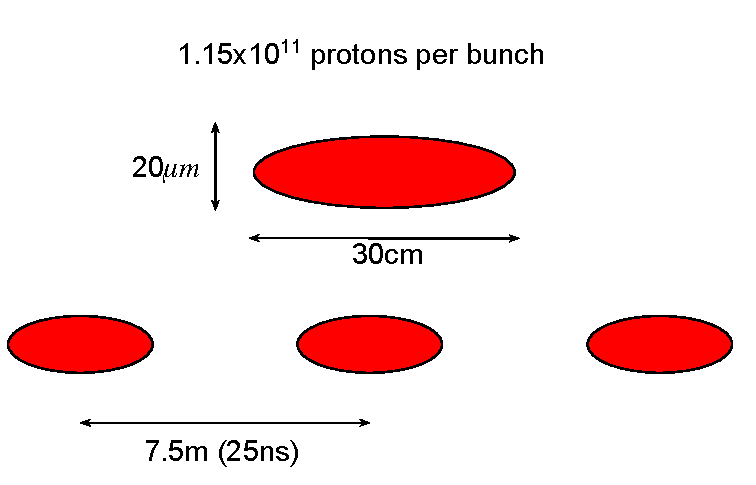
\includegraphics[width=0.49\linewidth]{Experiment/LHC/Image/lhc_bunchConf.pdf}}
    	\hfil
      	\subfigure[The crossing of the beams at the interaction point. 
    	\label{subfig:lhc_xangle}]
    	{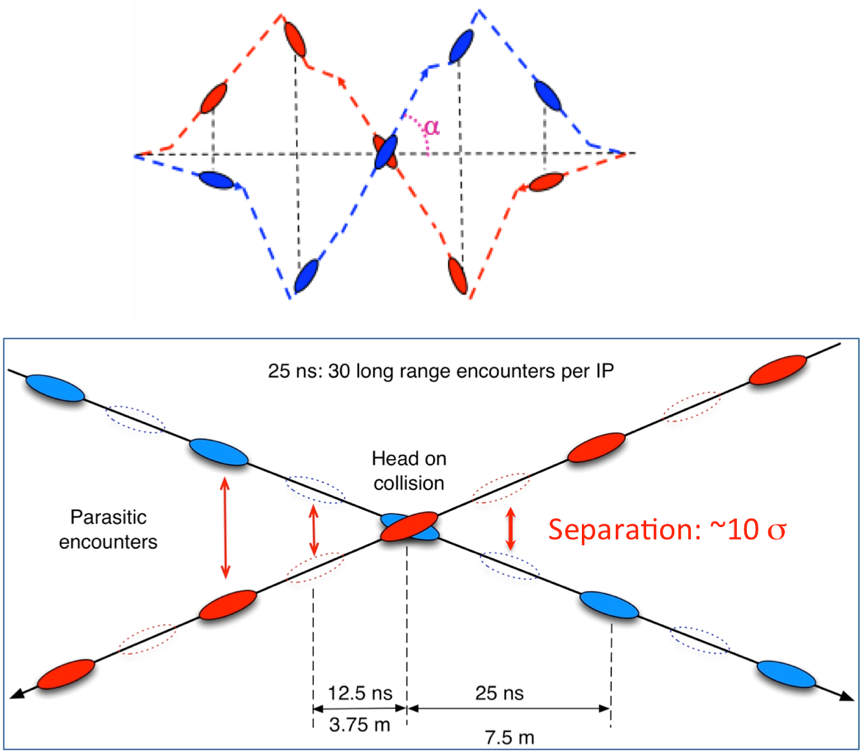
\includegraphics[width=0.49\linewidth]{Experiment/LHC/Image/lhc_xangle.png}}
      	\caption{The bunch configuration and crossing angle. The bunches are separated 
		by 7.5\unit{m}. The crossing angle shown is exaggerated for illustration.
		Figure~\ref{subfig:lhc_bunchConf} is adopted from \cite{CMSDAS} and 
		Figure~\ref{subfig:lhc_xangle} is taken from \cite{Mike}.}
    	\label{subfig:lhc_bunch_xangle}
      	\end{figure}
\item $\textbf{The $\beta^*$}$: The beam sizes do not remain constant throughout the 
	ring. Near the IP, the beams are bent using dipole magnets as shown in 
	Figure~\ref{fig:lhc_beamBend}. Therefore, the beams are a bit squeezed near the IP,  
	the extent of which is quantified with a parameter, called $\beta$. 
	The $\beta^*$ is $\beta$ value at IP. It is the distance from the IP up to a point 
	where the beam size is doubled. 
	The value of $\beta^*$ lies in the \unit{mm} range. Smaller value of $\beta^*$ 
	implies the beam is squeezed near the IP and vice-versa. The formula of $\beta^*$ 
	is given by~\cite{Baird:1017689}
     	\begin{equation}
     		\beta^* = \frac{\pi \sigma^2_{b}}{\epsilon}
     	\end{equation}
     	where $\sigma^2_{b}$ is the cross-sectional size of the bunch and 
	$\epsilon$ is the emittance, the smallest opening a beam
	can be squeezed through ~\cite{Baird:1017689}.
\item $\textbf{Center-of-mass energy ($\sqrt{s}$)}$: The counter rotating protons 
	collide head-on along the z-axis. In the center-of-mass frame, 
	$p_{1z} + p_{2z} = 0$. In addition, the momentum in the transverse plane must be conserved.
	If there is an imbalance in \pt, it would imply the production of some (unknown) particles 
	which has passed the detector without being detected; neutrino is an example. For the two 
	colliding protons with energy $E_1$ and $E_2$, the center-of-mass energy is given by 
	\begin{equation}
		\sqrt{s} = E_1 + E_2
	\end{equation}
     	For the 2016-18 data taking, the energy of each beam was 6.5 \TeV, leading to 
	$\sqrt{s}$ = 13 \TeV. The production of new particles in the physics
	process largely depends on $\sqrt{s}$. Higher the value of $\sqrt{s}$, more is
	the number of produced events for a given process. Many beyond the standard model 
	theories predict the existence of a new particle at higher $\sqrt{s}$. Therefore, 
	the $\sqrt{s}$ is an important parameter of the LHC.
\item $\textbf{Luminosity}$: Like the center-of-mass energy, luminosity is another important 
	parameter which is a measure of how many collisions occur.
	Higher luminosity means a higher chance of producing rare physics process in the
	collisions. With higher luminosity, the standard model predictions can be tested
	with more accuracy thanks to more statistics, hence less uncertainty. It is defined as:  
	\begin{equation}
		L = \frac{1}{\sigma_p}\frac{dR}{dt}
	\end {equation}
	where $\frac{dR}{dt}$ is the number of events per second and $\sigma_p$ is the cross section.
	In the \rm{CGS} unit, the dimension of $L$ is $\unit{cm}^{-2} \unit{s}^{-1}$. However,
	\fbinv (inverse femtobarn) is often used in the collider experiments.
	The luminosity is recorded by experiments over a certain period of time. The
	integrated luminosity is the integration of instantaneous luminosity over a period of time
	\begin{equation}
		L_{\rm{int}} =  \int L dt
	\end{equation}
	At the LHC, the luminosity is calculated in terms of beam parameters such as number of
	particles ($N$), collision frequency ($f$), the number of bunches in the beam ($N_b$), 
	etc \cite{Herr:941318}. 
	\begin{figure}
	  \begin{center}
	  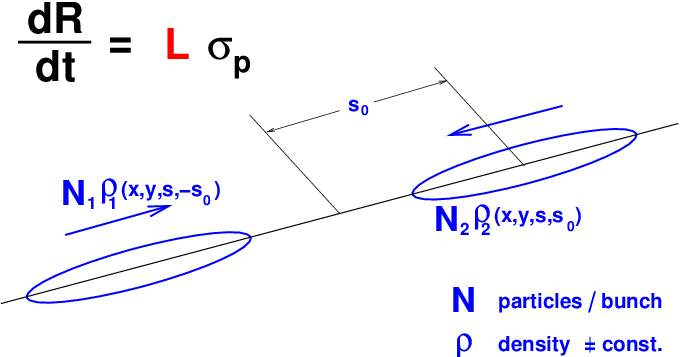
\includegraphics[width=0.50\linewidth]{Experiment/LHC/Image/lhc_lumi.png}
	  \caption{Two oppositely moving bunches with the total number of particles $N_1$ and
		  $N_2$, and beam density distribution functions $\rho_1(x, y, s, -s_0)$ and 
		  $\rho_2(x, y, s, s_0)$
		  \cite{Herr:941318}.}
	  \label{fig:lhc_lumi_rho}
	\end{center}
	\end{figure}
	For two counter rotating bunches with total number of particles 
	$N_1$ and $N_2$, and beam density distribution functions $\rho_1(x, y, s, -s_0)$ and 
	$\rho_2(x, y, s, s_0)$ as shown in Figure~\ref{fig:lhc_lumi_rho}, the luminosity is given 
	by~\cite{Herr:941318} 
	\begin{equation}
		L =  2N_1N_2fN_b\int\int\int\int \rho_1(x, y, s, -s_0) 
		\rho_2(x, y, s, s_0) dxdydsds_0.
	\label{eq:lhc_lumi1}
	\end{equation}
	where $s$ corresponds to the $z$-coordinate which is along the beam direction and $s_0$ is
	the $4^{\rm{th}}$ component of space-time coordinate, that is, $s_0 = ct$. As shown in 
	Figure~\ref{fig:lhc_lumi_rho}, the two bunches meet at $s_0 = 0$. Assuming that the two
	bunches collide head-on and the beam density is uncorrelated along all directions, 
	Equation (\ref{eq:lhc_lumi1}) can be written as
	\begin{equation}
		L =  2N_1N_2fN_b\int\int\int\int \rho_{1x}(x)\rho_{1y}(y)
		\rho_{1s}(s-s_0)\rho_{2x}(x)\rho_{2y}(y)\rho_{2s}(s+s_0) dxdydsds_0.
	\label{eq:lhc_lumi2}
	\end{equation}
 	The beam density distribution at the LHC follows a Gaussian distribution, that is, the 
	proton density is more in the middle of the beam and lesser as one goes away from the
	middle point. Therefore, for the two beams, the beam density functions in 
	Equation (\ref{eq:lhc_lumi2}) can be written as
	\begin{equation}
		\rho_{ix}(x) = \frac{1}{\sigma_{ix}\sqrt{2\pi}}
		\exp\left(-\frac{(x)^2}{2\sigma_{ix}^2}\right), i = 1, 2
	\end{equation}
	\begin{equation}
		\rho_{iy}(x) = \frac{1}{\sigma_{iy}\sqrt{2\pi}}
		\exp\left(-\frac{(y)^2}{2\sigma_{iy}^2}\right), i =1, 2
	\end{equation}
	\begin{equation}
		\rho_s(s\pm s_0) = \frac{1}{\sigma_s\sqrt{2\pi}}
		\exp\left(-\frac{(s\pm s_0)^2}{2\sigma_s^2}\right)
	\end{equation}
	where $\sigma_{ix}$ and $\sigma_{iy}$ are the standard deviation of Gaussian distribution 
	of the two beams along the $x$ and $y$-direction. Using these, Equation (\ref{eq:lhc_lumi2}) 
	becomes \cite{Herr:941318}
	\begin{equation}
		L = \frac{N_1N_2fN_b}{2\pi\sqrt{\sigma_{1x}^2 + \sigma_{2x}^2}
		\sqrt{\sigma_{1y}^2 + \sigma_{2y}^2}}
	\label{eq:lhc_lumi}
	\end{equation}
        Equation (\ref{eq:lhc_lumi}) holds in the ideal situation where the beam profile 
	is uncorrelated in all directions and the machine operates in an ideal condition. However 
	in real life, there are various additional machine effects that need to be 
	incorporated such as finite crossing angle, collision offset, hourglass effect, non-Gaussian 
	beam profiles, nonzero dispersion at the collision point, and so on ~\cite{Herr:941318}. 
	The luminosity given by Equation (\ref{eq:lhc_lumi}) is what delivered by the LHC. Each 
	detector records the luminosity individually during the collision. The recorded luminosity 
	is always smaller than the delivered one due to the detector effects. Five sub-detectors of 
	the CMS experiment are used to monitor and measure the luminosity. These are the silicon 
	pixel detector, the Hadron Forward Calorimeter (HF), the Drift Tubes in the barrel (DT), 
	Pixel Luminosity Telescope (PLT), and  the Fast Beam Conditions Monitor 
	(BCM1f)~\cite{CMS-PAS-LUM-15-001}.

	The luminosity delivered by the LHC and recorded by CMS for 2016 data taking is shown 
	in Figure~\ref{fig:lhc_lumi_2016} over a period of time. The integrated 
	recorded luminosity is 37.8\fbinv for the 2016 data taking. However, a luminosity
	mask is applied to reject some amount where some parts of the CMS detector 
	were not operating in the normal mode. Accordingly, the recorded
	luminosity reduced to 35.9\fbinv. The analysis of 2016 data is what presented in this thesis.
	Delivered luminosity for different center-of-mass energies and during different years
	are shown in Figure~\ref{fig:lhc_lumi_allYear}. The total delivered luminosity at
	13 \TeV during 2015-18 is about 160\fbinv.
	\begin{figure}
       	\centering
      	\subfigure[Delivered luminosity by the LHC and recorded by CMS in 2016 data taking. 
      	\label{fig:lhc_lumi_2016}]
      	      {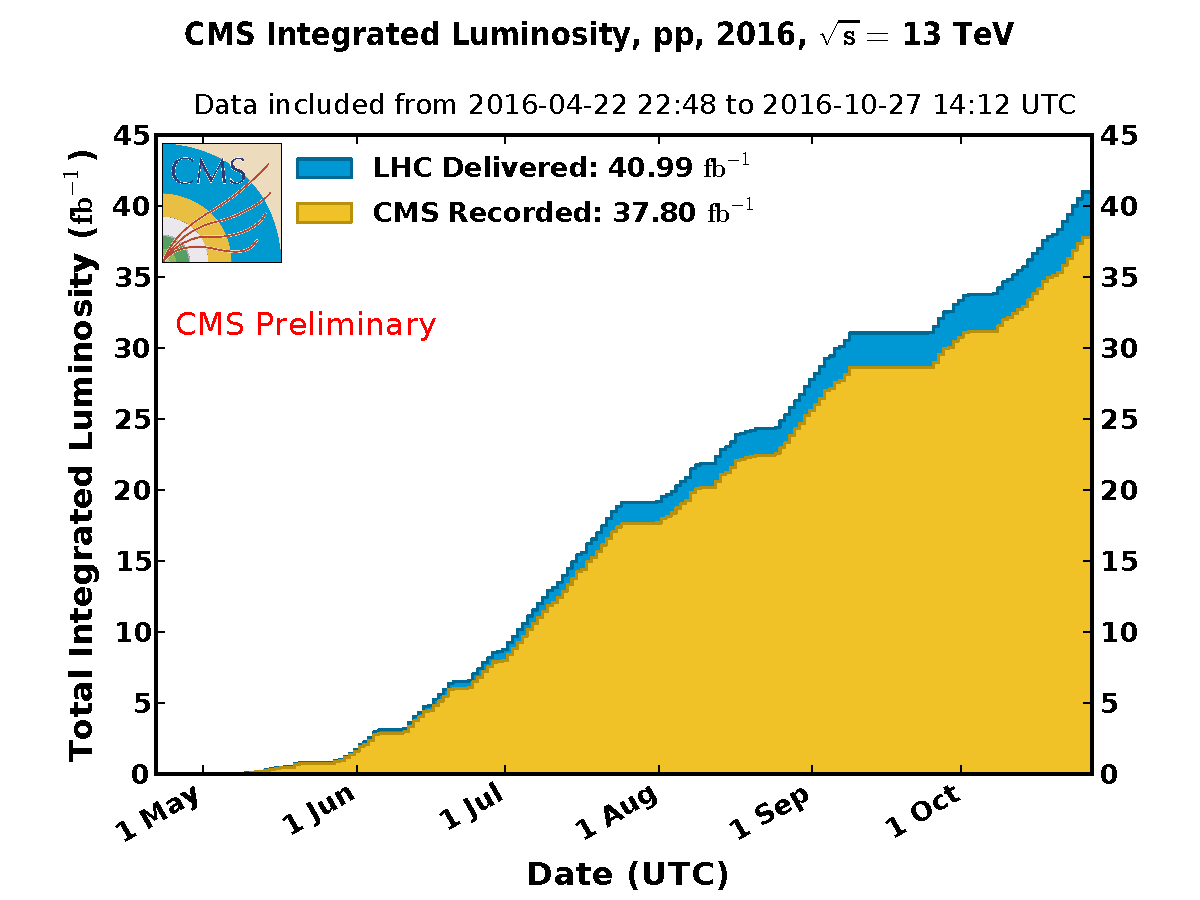
\includegraphics[width=0.49\linewidth]{Experiment/LHC/Image/lumi_2016.pdf}}
      	\hfil
      	\subfigure[Delivered luminosity by the LHC for different years at the different 
	center-of-mass energies, starting from 2010 to 2018.
      	\label{fig:lhc_lumi_allYear}]
	{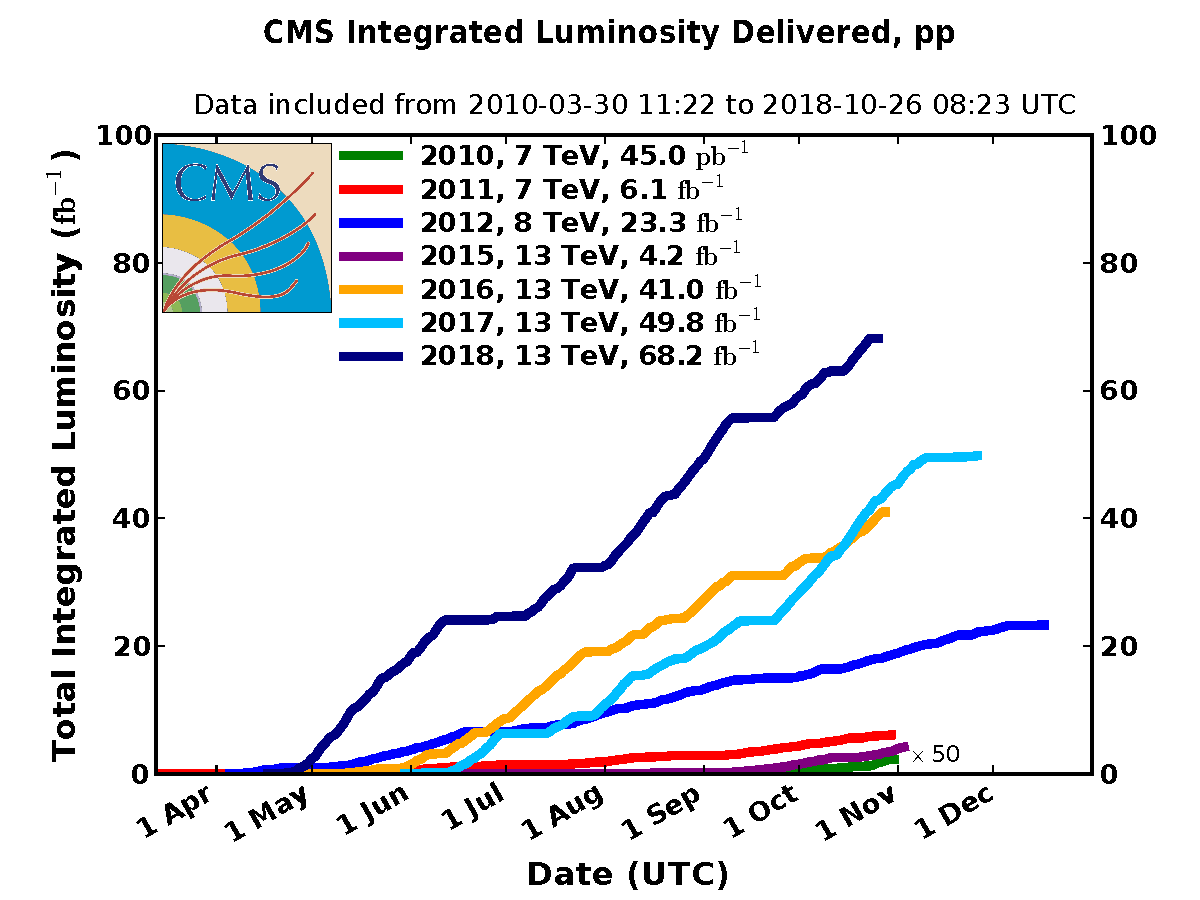
\includegraphics[width=0.49\linewidth]{Experiment/LHC/Image/lumi_allYear.pdf}}
	\caption{Luminosity measurement from different years of the data taking \cite{CMSLumi}. 
		In this thesis, the analysis presented uses the one for the 2016 data taking
		(golden yellow line in the right plot). The total delivered luminosity at 13 \TeV 
		from all years is about 160\fbinv.}
      	\label{fig:lhc_lumi}
     	\end{figure}
\end{itemize}
At the LHC, there are various beam modes indicating the beam status such as 
\dq{Squeeze} (the beams are squeezed by betatron towards the target collision, for most of
the 2016 data taking the $\beta^*$ = 30\unit{cm}), \dq{Adjust} (the separation between the beams
is made to collapse, bringing them for collision), \dq{Stable beams} (it signals that
the physics data taking can be started), and \dq{Dump} (the beams are dumped after the data
taking ends). The stable beam mode lasts for a few hours during which the collisions are recorded.

A \dq{Fill} is created as soon as the stable beams are achieved and all the detector information
is updated in the online database. A Fill lasts for few hours and is divided in 
\dq{Runs} for better management. Further, a Run is divided in \dq{lumi sections}. The duration
of each lumi section (LS) is 23\unit{s}. Therefore, the data taking by a detector has a granularity
of 23\unit{s}. That is, the detector information is updated/stored after each 23\unit{s}. An LS 
is marked as good or bad depending on whether all the parts of the detector were
on or some of them were off. The integrated luminosity is obtained by summing over all LS.

All the LHC parameters are measured regularly during the data taking. Most of them
do not change on a regular day-to-day basis. However, few do change on every day during the data
taking such as the ones shown in Figure~\ref{fig:lhc_param_day}. Other parameters change over
a period of time, for example on a month-to-month basis, and some even on a yearly basis
such as the ones shown in Figure~\ref{fig:lhc_param_month}.

\begin{figure}
  \begin{center}
  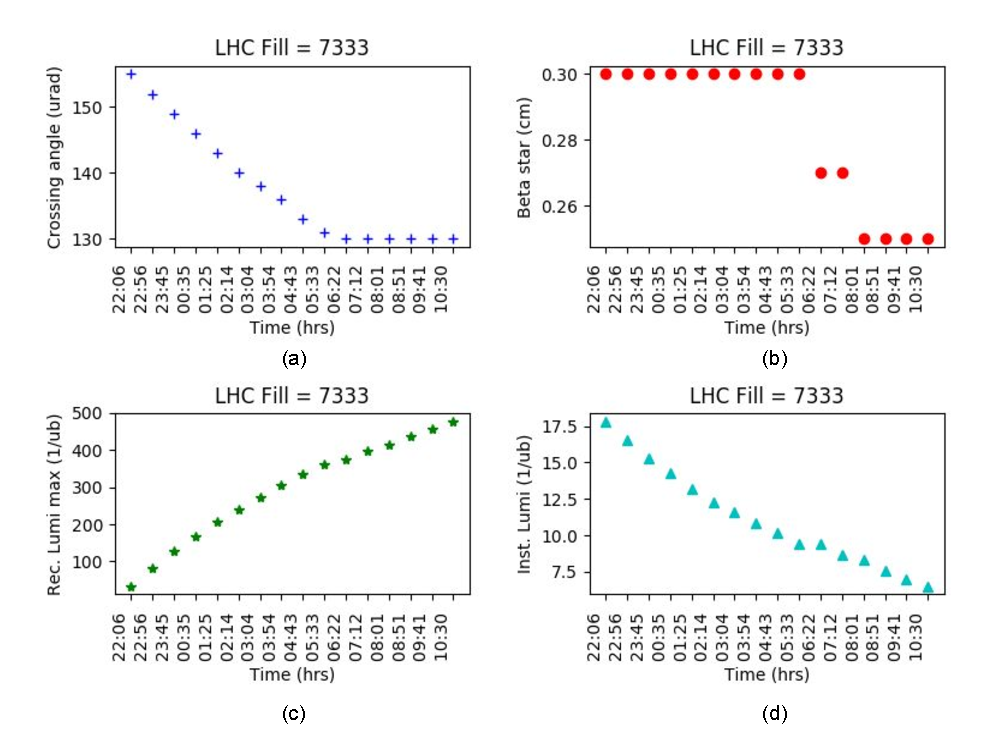
\includegraphics[width=0.70\linewidth]{Experiment/LHC/Image/lhc_param_day.pdf}
  \caption{Variation of few LHC parameters during the data taking on 22-23rd October
	  2018 (Fill = 7333). All these parameters change over a different point of time.
	  Other parameters such as the center-of-mass energy, number of particles in 
	  each beam, etc do not change on a given day.
	  }
  \label{fig:lhc_param_day}
  \end{center}
\end{figure}
\begin{figure}
  \begin{center}
  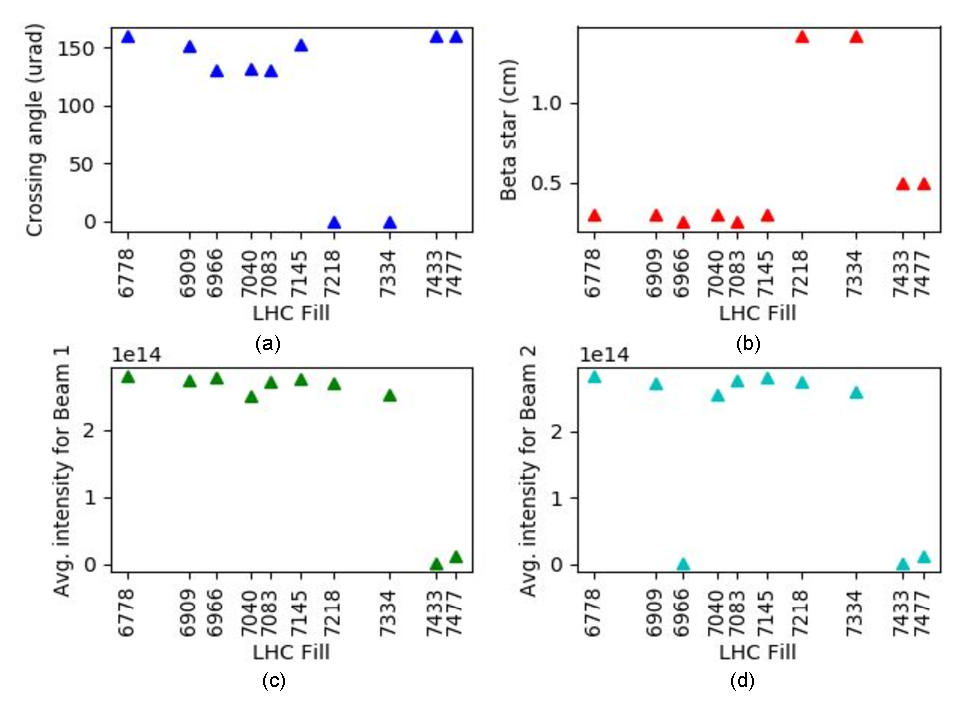
\includegraphics[width=0.70\linewidth]{Experiment/LHC/Image/lhc_param_month.pdf}
  \caption{Variation of few LHC parameters during the data taking from random days in
	  the period of June-November 2018. Only a few days (Fills) have been chosen for
	  illustration. The last two Fills (7433 and 7477) correspond to Pb-Pb, 
	  rest are from proton-proton collisions. The average intensity of the beam is the 
	  number of particles in each beam. As can be seen, all these parameters change over 
	  a different period of time.
	  }
  \label{fig:lhc_param_month}
  \end{center}
\end{figure}

\section{The LHC coordinate system}
\label{s:lhc_cord}
Most of the detectors placed at the IRs have a cylindrical shape with the axis of
the cylinder lying along the beam direction. Within the detectors, various sub-detectors are placed
either parallel (barrel region) to the beam direction or perpendicular (endcap region) to it.
At the LHC, the $z$-axis lies along the beam direction, while the $x$-$y$ plane is perpendicular 
to it as shown in Figure~\ref{fig:lhc_cord}. 
%https://wiki.physik.uzh.ch/cms/latex:example_spherical_coordinates
\begin{figure}
  \begin{center}
  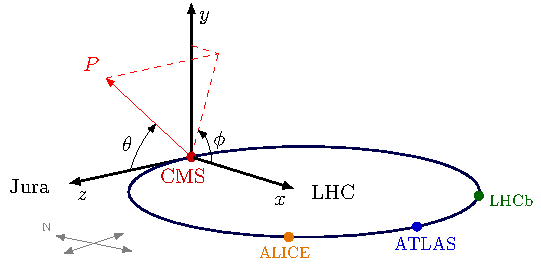
\includegraphics[width=0.50\linewidth]{Experiment/LHC/Image/cord.pdf}
  \caption{The LHC coordinate system \cite{CMSWiki} with the $z$-axis lying along the beam direction. 
	At CMS, the $z$-axis points towards the mountain Jura in France.}
  \label{fig:lhc_cord}
  \end{center}
\end{figure}
The following derived quantities are often used by the LHC experiments:
\begin{itemize}[leftmargin=*]
\item $\textbf{Transverse momentum (\pt)}$: 
	Out of $10^{11}$ protons in a bunch, only about 20 hard collisions occur 
	in one bunch crossing. Rest of the protons move in the forward region, some of 
	them with soft collision and some even without being collided. The hard 
	collisions produce actual physics process of interest. Due to the head-on 
	collision, the particles produced in hard collisions mostly go in the transverse 
	plane. The momentum in the $x$-$y$ plane, \pt, is defined as
	\begin{equation}
		\pt = \sqrt{p_x^2 + _y^2}
	\end{equation}
	where $p_x$ and $p_y$ are the $x$ and $y$ components of the momentum vector, respectively. 
	Detecting a higher \pt in an event indicates the occurrence of actual physics process.
\item $\textbf{Pseudorapidity $(\eta)$}$: As shown in Figure~\ref{fig:lhc_cord}, 
	the azimuthal angle ($\phi$) is the angle between $\vec{p_x}$ and the $x$-axis. 
	It covers the full barrel region and ranges from 0 to 2$\pi$. On the other hand $\theta$ 
	is the angle between the momentum vector $\vec{p}$ and $z$-axis which varies from 0 to 
	$\pi$ to cover both sides of the endcap. 
	In the collider experiments, one measures 4-vector ($E, \vec{p}$) of a 
	particle. Just looking at the 4-vector, its not easy to predict the direction
	of the particle with respect to the beam axis. In view of this, there is a quantity 
	called \dq{rapidity}, given by \cite{EDaw}
	\begin{equation}
		y = \frac{1}{2}\ln\left(\frac{E+p_z}{E-p_z}\right)
	\label{eq:lhc_y}
	\end{equation}
	which is very useful to know the value of $\theta$. For example, $y = 0$ implies 
	that $E > p_z$. That is, the particle is produced in the transverse plane which
	implies $\theta = \pi/2$. For $y = \pm 1$, $E<p_z$. That is the particle is
	moving mostly in the beam direction implying $\theta = 0$ or $\pi$. The
	another advantage of rapidity is that the difference in rapidities is Lorentz 
	invariant. For example, under the Lorentz boost, the 4-momentum transforms as 
	$E^\prime = \gamma (E-\beta p_z) , ~p^\prime_x = p_x, ~p^\prime_y = p_y, ~p^\prime_z = \gamma(p_z - \beta E)$, so the rapidity is transformed as
	\begin{equation}
		y^\prime = y - \tanh^{-1}\beta
	\end{equation}
	where $\beta = v$ ($v$ is the velocity of the boosted frame), and 
	$\gamma = \sqrt{1-\beta^2}$. If an observer measures rapidities of two particles
	in the boosted frame then difference $y_1^\prime -y_2^\prime = y_1 - y_2$.
	That is, the difference in rapidities is Lorentz invariant. This is very useful
	when one is interested in the angular separation between two physics objects such
	as a muon and a hadronic jet.

	The relativistic limit of rapidity is called pseudorapidity ($\eta$). In such limit, 
	the momentum of a particle is much larger than its rest mass 
	, that is, $E = \sqrt{p^2 + m_0^2} \approx p$. Therefore, Equation (\ref{eq:lhc_y}) becomes
	\begin{equation}
		y = - \ln\tan \left(\frac{\theta}{2}\right) \to \eta
	\label{lhc_eta}
	\end{equation}
	The $\eta$ variable is mostly used everywhere at the LHC as it is directly related to the
	angle $\theta$. The relationship between $\eta$ and $\theta$ is shown in Figure 
	\ref{fig:lhc_eta}.
	%https://en.wikipedia.org/wiki/Pseudorapidity
	\begin{figure}
	\begin{center}
	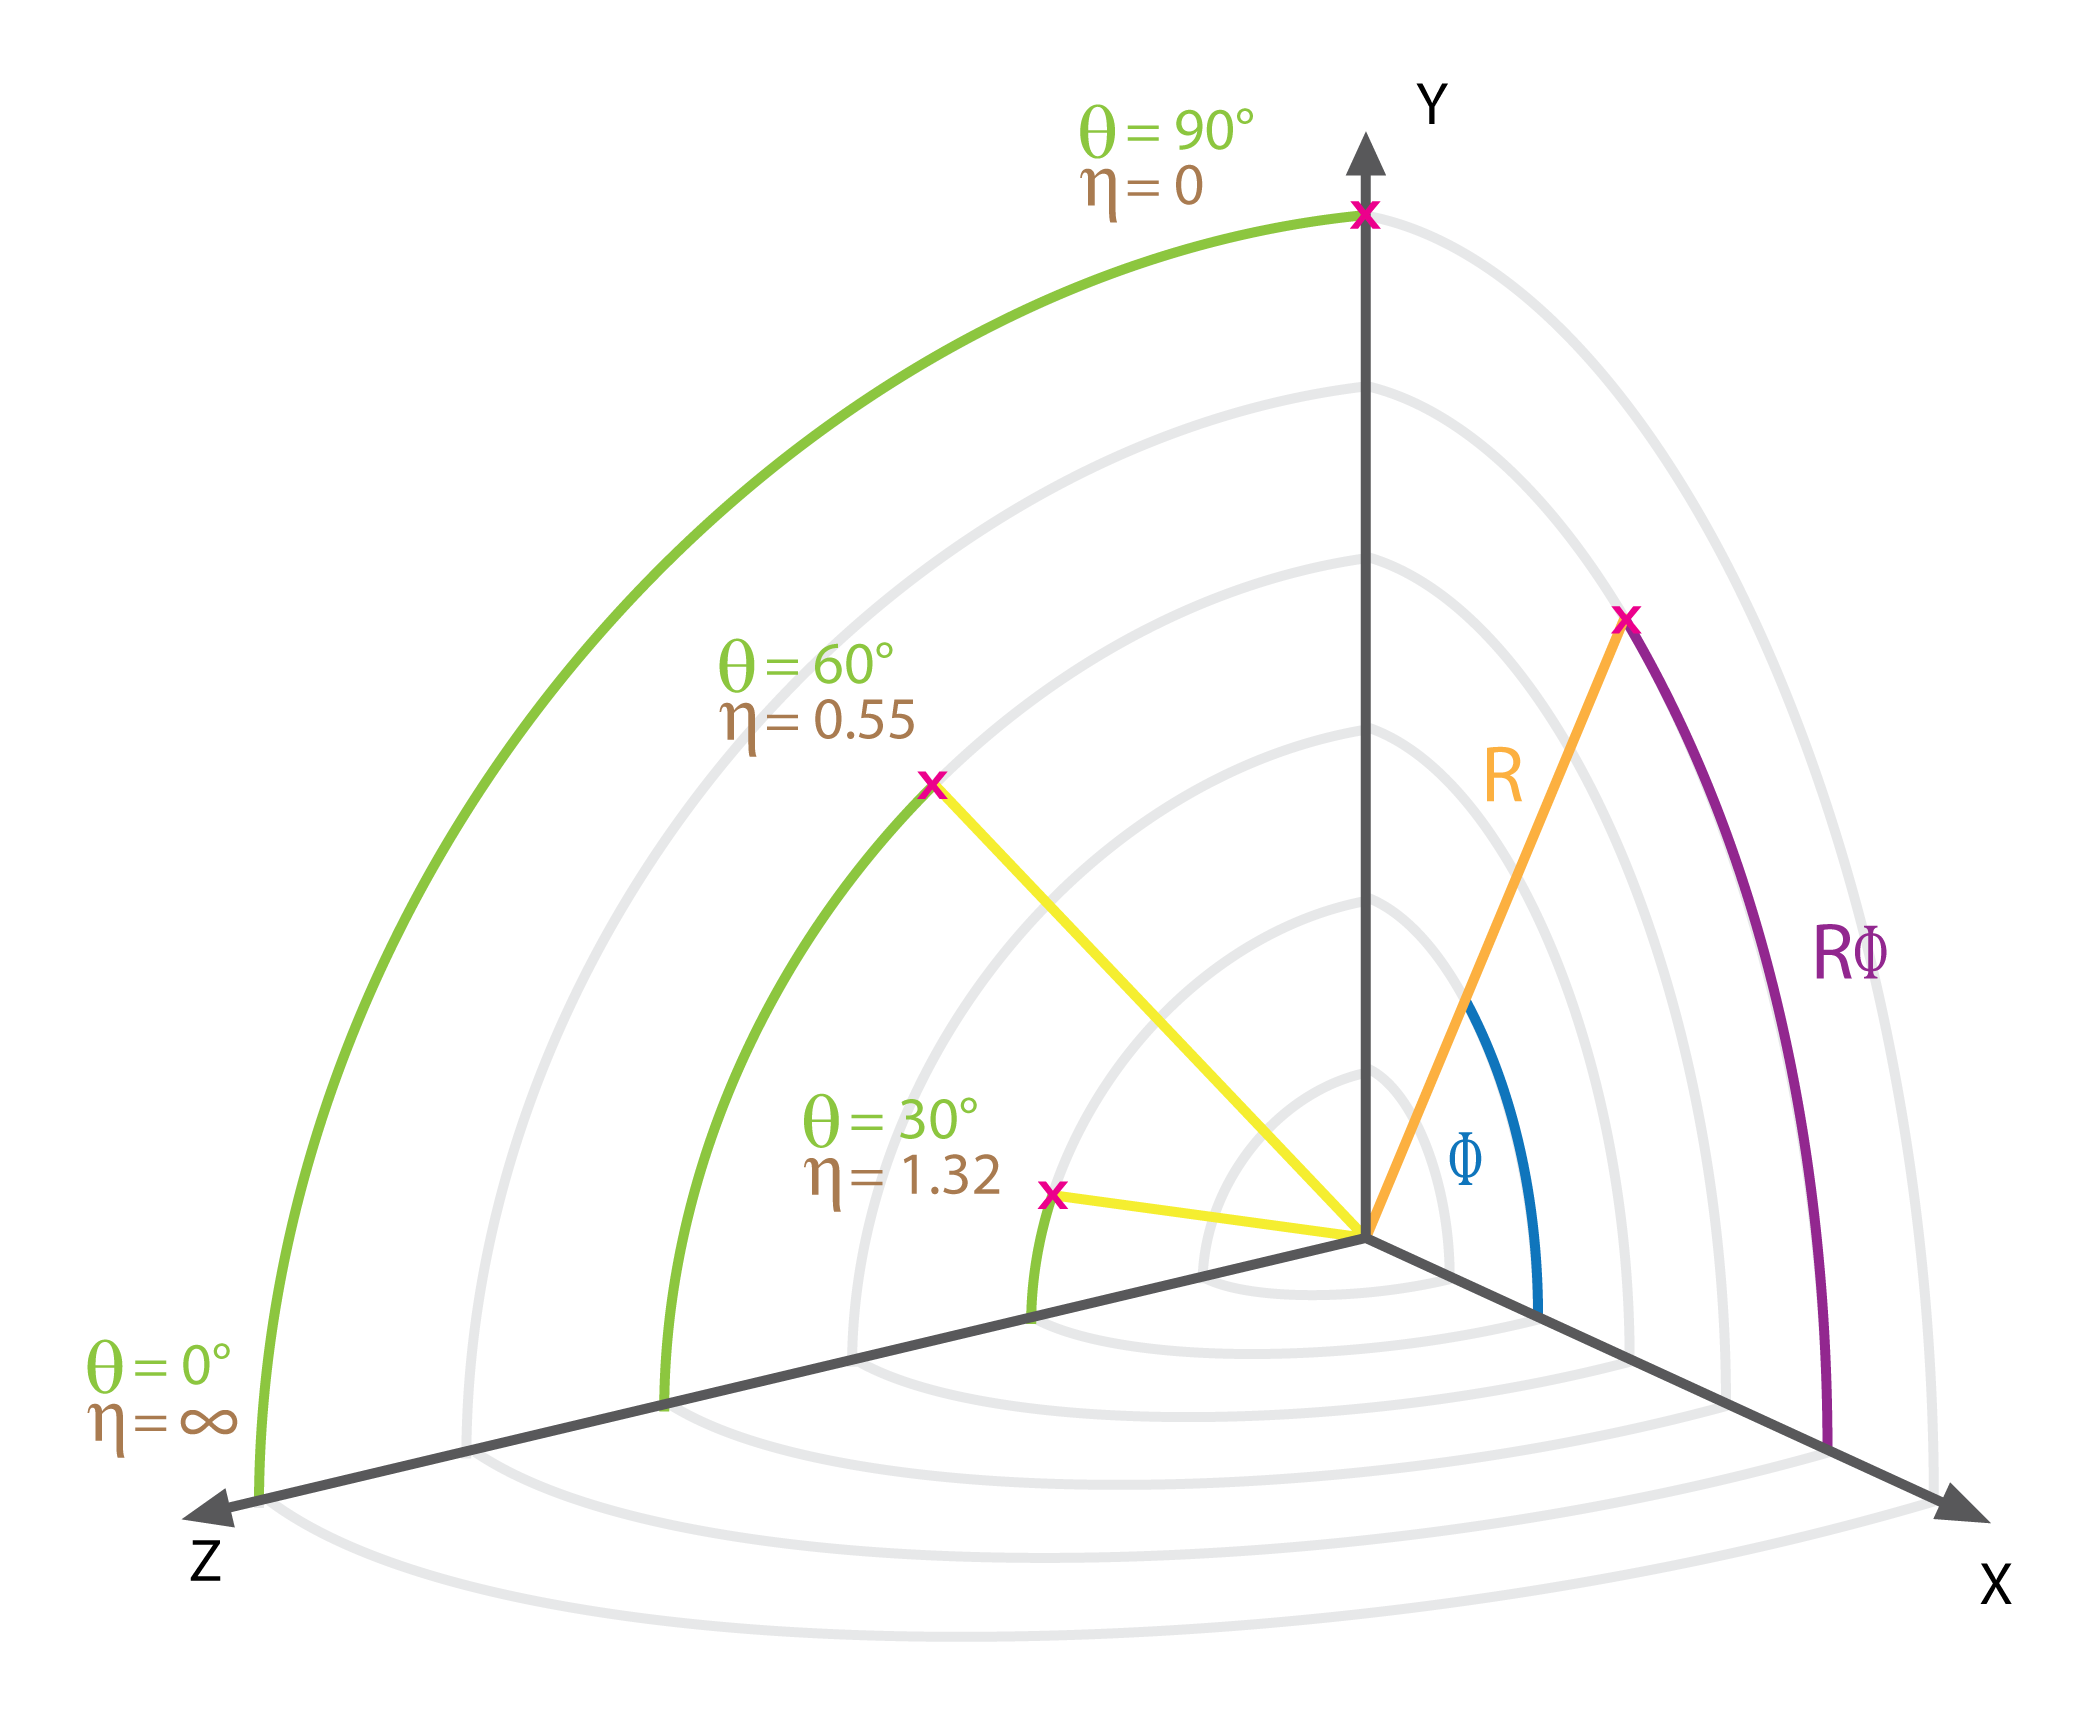
\includegraphics[width=0.50\linewidth]{Experiment/LHC/Image/lhc_eta.png}
		\caption{The relationship between $\theta$ and $\eta$ \cite{Lenzi:2013xpa}. The 
	value of $\eta = 0$ implies $\theta = \pi/2$. That is, lower the value of $\eta$ the farther 
	away we are from the beam axis in the perpendicular direction and vice versa.}
	\label{fig:lhc_eta}
	\end{center}
	\end{figure}
	One can see that for a large value of $\eta$, \eg, $\eta = 4 (-4)$, the particle is 
	close to the beam axis [$\theta = 0 (\pi)$]. Similarly, the lower value of $\eta$ indicates 
	that the particle is produced in the transverse plane. The lower and higher values of
	$\eta$ correspond to barrel and endcap region of the detector, respectively.
\end{itemize}


\chapter{The CMS Experiment at The LHC}
\label{c:secCMS}
\section{Introduction}
\label{s:secIntroCMS}
\begin{figure}
  \begin{center}
  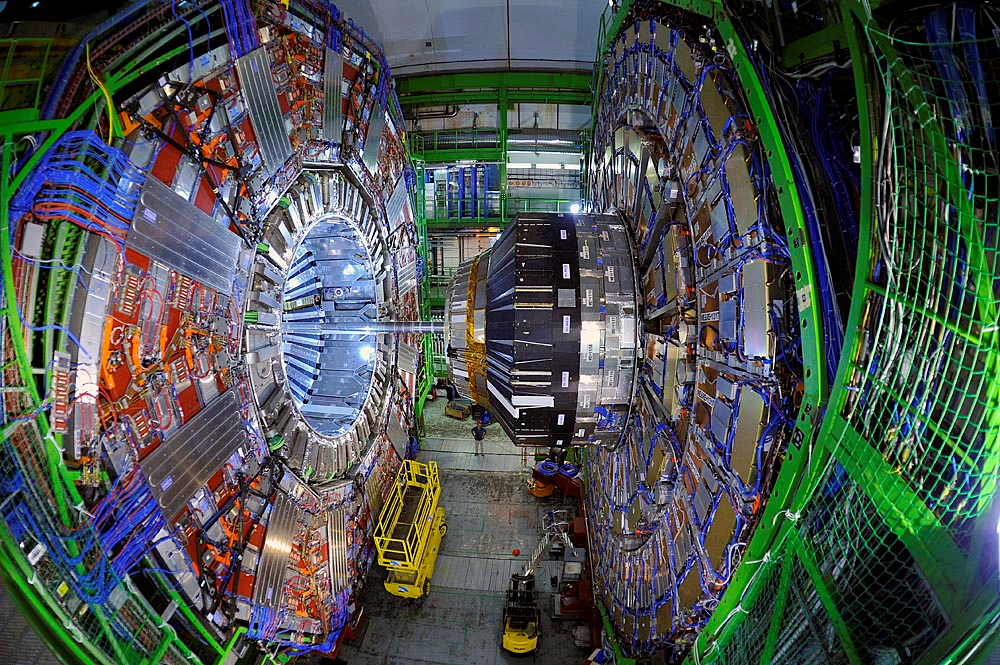
\includegraphics[width=0.90\linewidth]{Experiment/CMS/Image/cms.png}
  \caption{The CMS detector installed in IR5 at the LHC~\cite{Collaboration_2008_CMS}.}
  \label{fig:cms_exp}
  \end{center}
\end{figure}
The Compact Muon Solenoid (CMS) detector is installed in IR5 at the LHC ring. 
CMS is one of the biggest international collaborations involving 43 countries, 
199 institutes, with around 4000 people. The weight of the CMS detector is about 
14000 tonnes (around the weight of 2500 African elephants). Such a huge weight is 
accommodated in a small volume (the shape of CMS is cylindrical with length of 
21.5\unit{m}, and diameter of 15.6\unit{m}). That is why the \dq{compact} word has been 
attached to it. One of the main physics goals of the CMS experiment is to detect \dq{muons} 
as they are produced in most of the Standard Model processes. Of course, other particles 
such as an electron, photon, neutral and charged hadrons are also detected. A huge 
\dq{solenoid} magnet is placed inside the CMS to bend the tracks of charged particles so that 
their momentum can be measured precisely. An image of the CMS experiment is shown
in Figure~\ref{fig:cms_exp}, while various parts of the detectors are shown in Figure
\ref{fig:cms_diag}. The beam axis is along the center of the cylinder. The 
tracker (silicon pixel and strip) is the first sub-detector followed by the 
electromagnetic calorimeter (ECAL), and the hadron calorimeter (HCAL). The
magnetic solenoid is placed outside the HCAL followed by the muon chambers.
The iron yoke provides stand for the muon chambers and contains the magnetic 
flux outside the solenoid. A detailed description of each 
sub-detector is given in the next sections. 

The trajectories of various particles inside the CMS detector are shown in Figure
\ref{fig:cms_track}. The particles are produced at the IP and
move towards various layers of the detector. The charged particles are bent
thanks to the presence of a strong magnetic field inside the solenoid. Outside of it, 
the charged particles are bent in the opposite direction. On the other hand, the neutral particles 
do not bend inside the detector. The particles detected by the CMS experiment are 
muon, electron, charged hadron (e.g. pion), neutral hadron (e.g. neutron), and photon.
\begin{figure}
  \begin{center}
  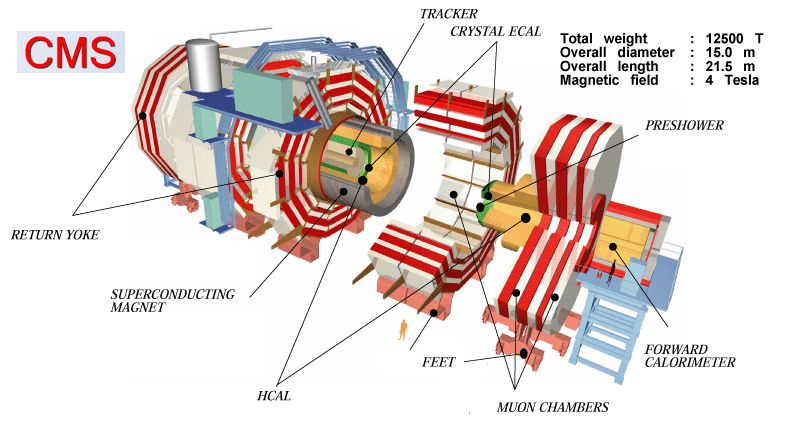
\includegraphics[width=0.90\linewidth]{Experiment/CMS/Image/cmsdiag.png}
	  \caption{Diagram of the CMS detector \cite{cmsDiagram}. Various parts 
	  of the CMS detector are shown starting from tracker to ECAL to HCAL to magnet to 
	  the muon chambers.}
  \label{fig:cms_diag}
  \end{center}
\end{figure}
%Fig\pdfcomment[author={FIG COURTESY}]{http://physics.stackexchange.com/questions/139540/how-detectors-in-particle-colliders-can-differentiate-neutrons-from-antineutrons}}
\begin{figure}
  \begin{center}
  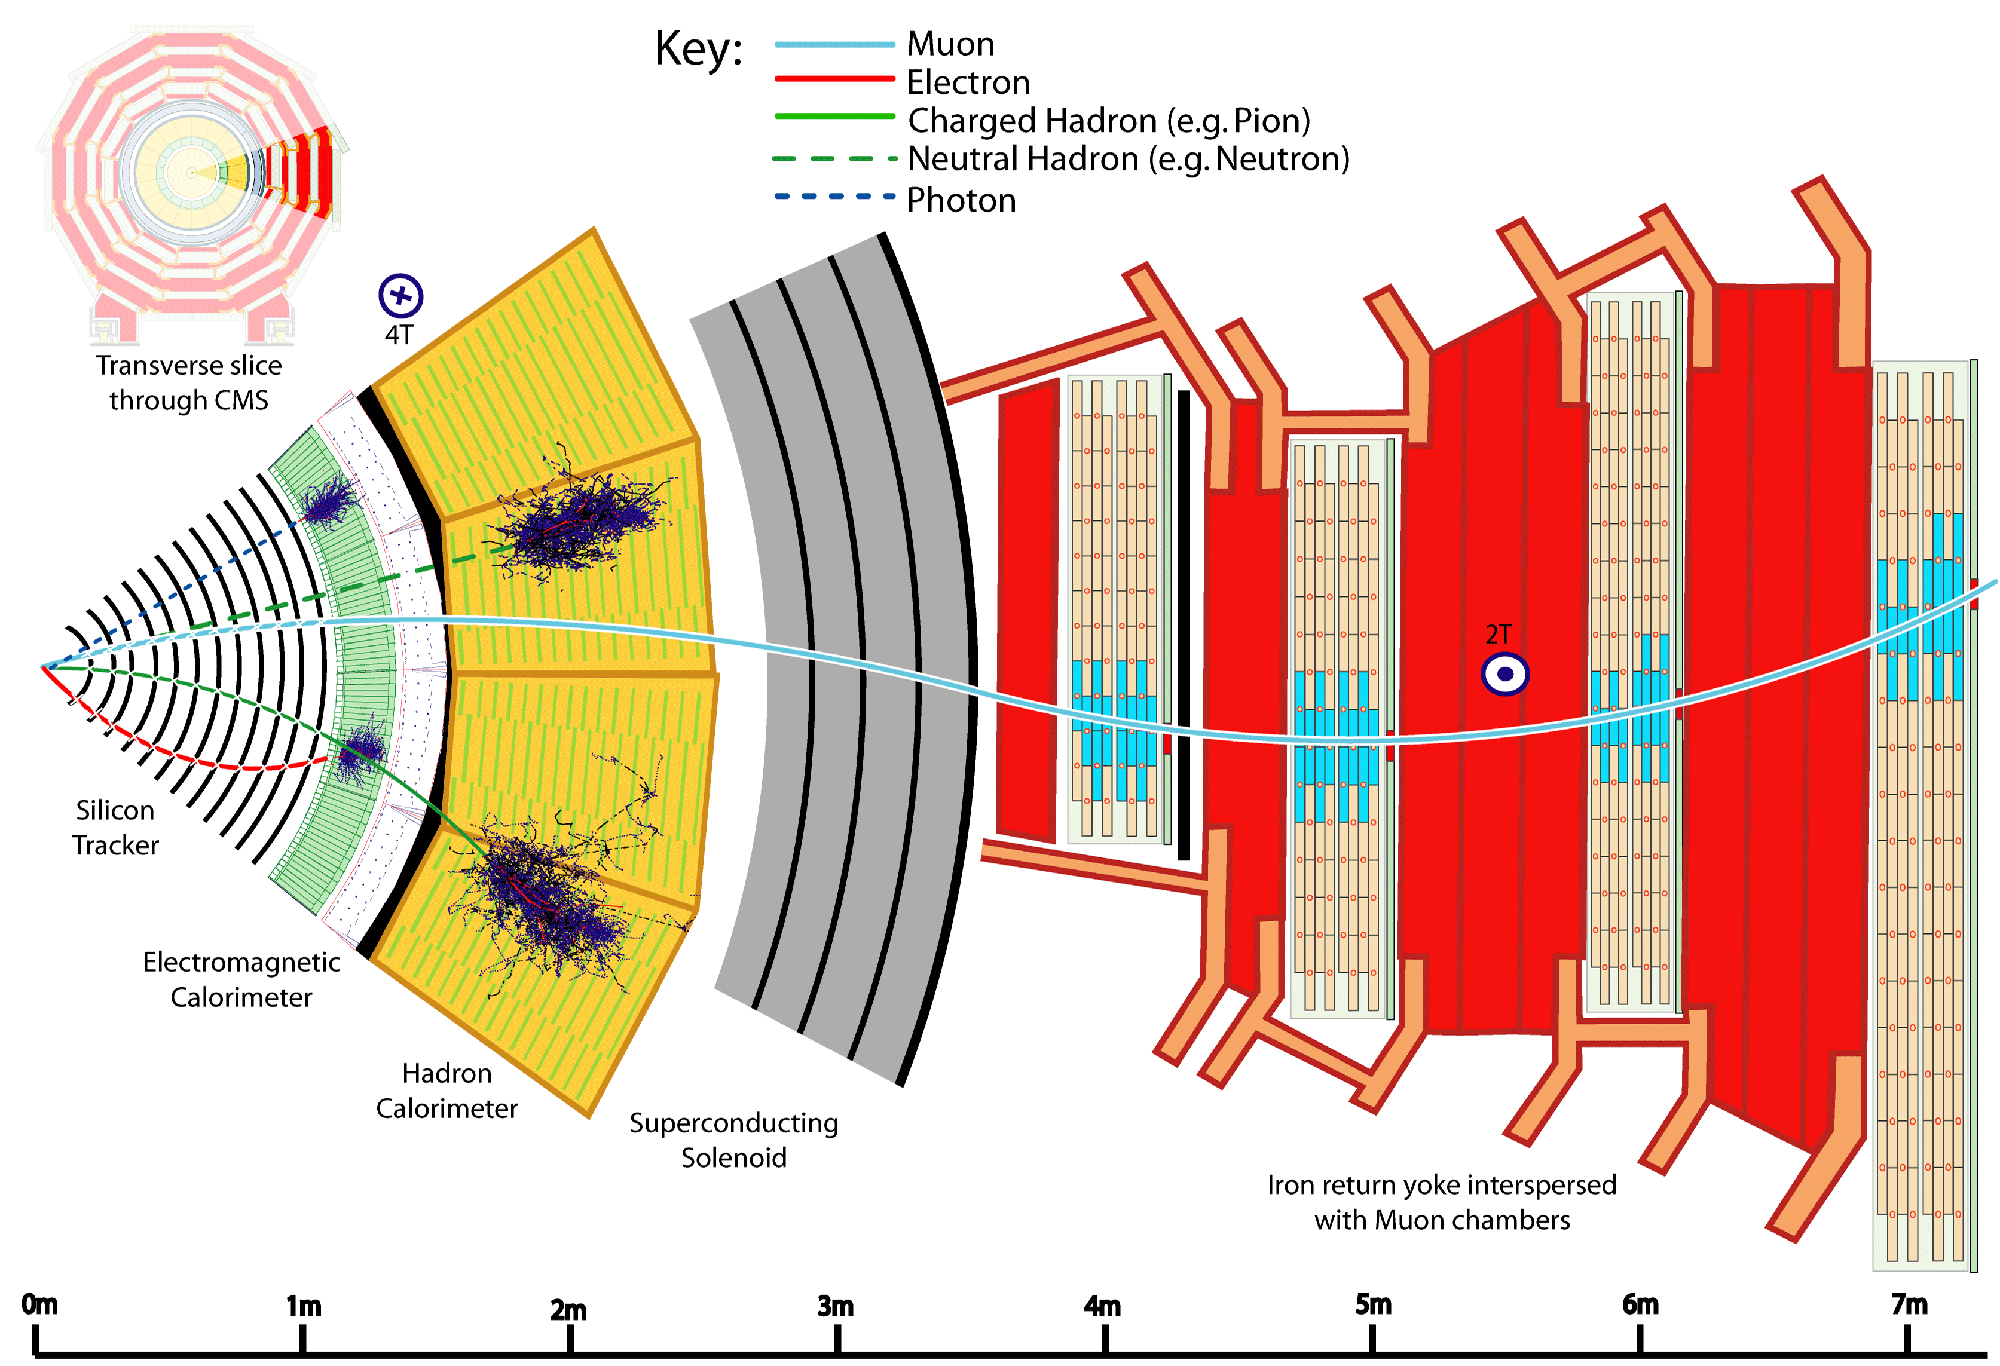
\includegraphics[width=0.90\linewidth]{Experiment/CMS/Image/cmstrack.png}
	  \caption{Trajectories of various particles inside the CMS detector 
	  \cite{Sirunyan:2270046}. The charged particles
	  such as electrons, muons, and charged pions ($\pi^\pm$) are bent inside and 
	  outside the
	  solenoid whereas the neutral particles such as photons and neutral pions ($\pi^0$)
	  traverse without being bent. The silicon tracker is mainly for measuring
	  the momentum of particles whereas the ECAL and HCAL measure the 
	  energy deposits. The electrons and photons deposit their energy inside the 
	  ECAL whereas the hadrons deposit in both ECAL and HCAL. The muons are the
	  only particles that traverses all the way to the muon chambers.}
  \label{fig:cms_track}
  \end{center}
\end{figure}


\section{Silicon tracker}
\label{ss:cms_tracker}
Due to the small band gap (1.12\unit{eV}), high carrier mobility (1450 \unit{$\rm{cm}^2/Vs$}), 
and high specific density (2.33 \unit{$\rm{g}/\rm{cm}^3$}) the silicon detectors are used in 
the CMS experiment for the measurements of trajectory and momentum of the particles 
produced in the collision.
The silicon tracker of the CMS is closest to the beam axis. Its location is shown in 
Figure~\ref{fig:cms_tracker}. It has 3 (2) layers of pixel tracker in the barrel (endcap) region, and
10 (9) layers of the strip tracker in the barrel (endcap) region. There are about 48 
(18) million pixels in the barrel (endcap) region covering an area of 200\unit{$\rm{m}^2$} which
makes it the biggest silicon detector ever built in the world.
\begin{figure}
  \centering
  \subfigure[The inner part of one of the tracker inner barrels (TIBs) of the
	CMS experiment \cite{cmsInfo}.
  \label{subfig:cms_track}]
  {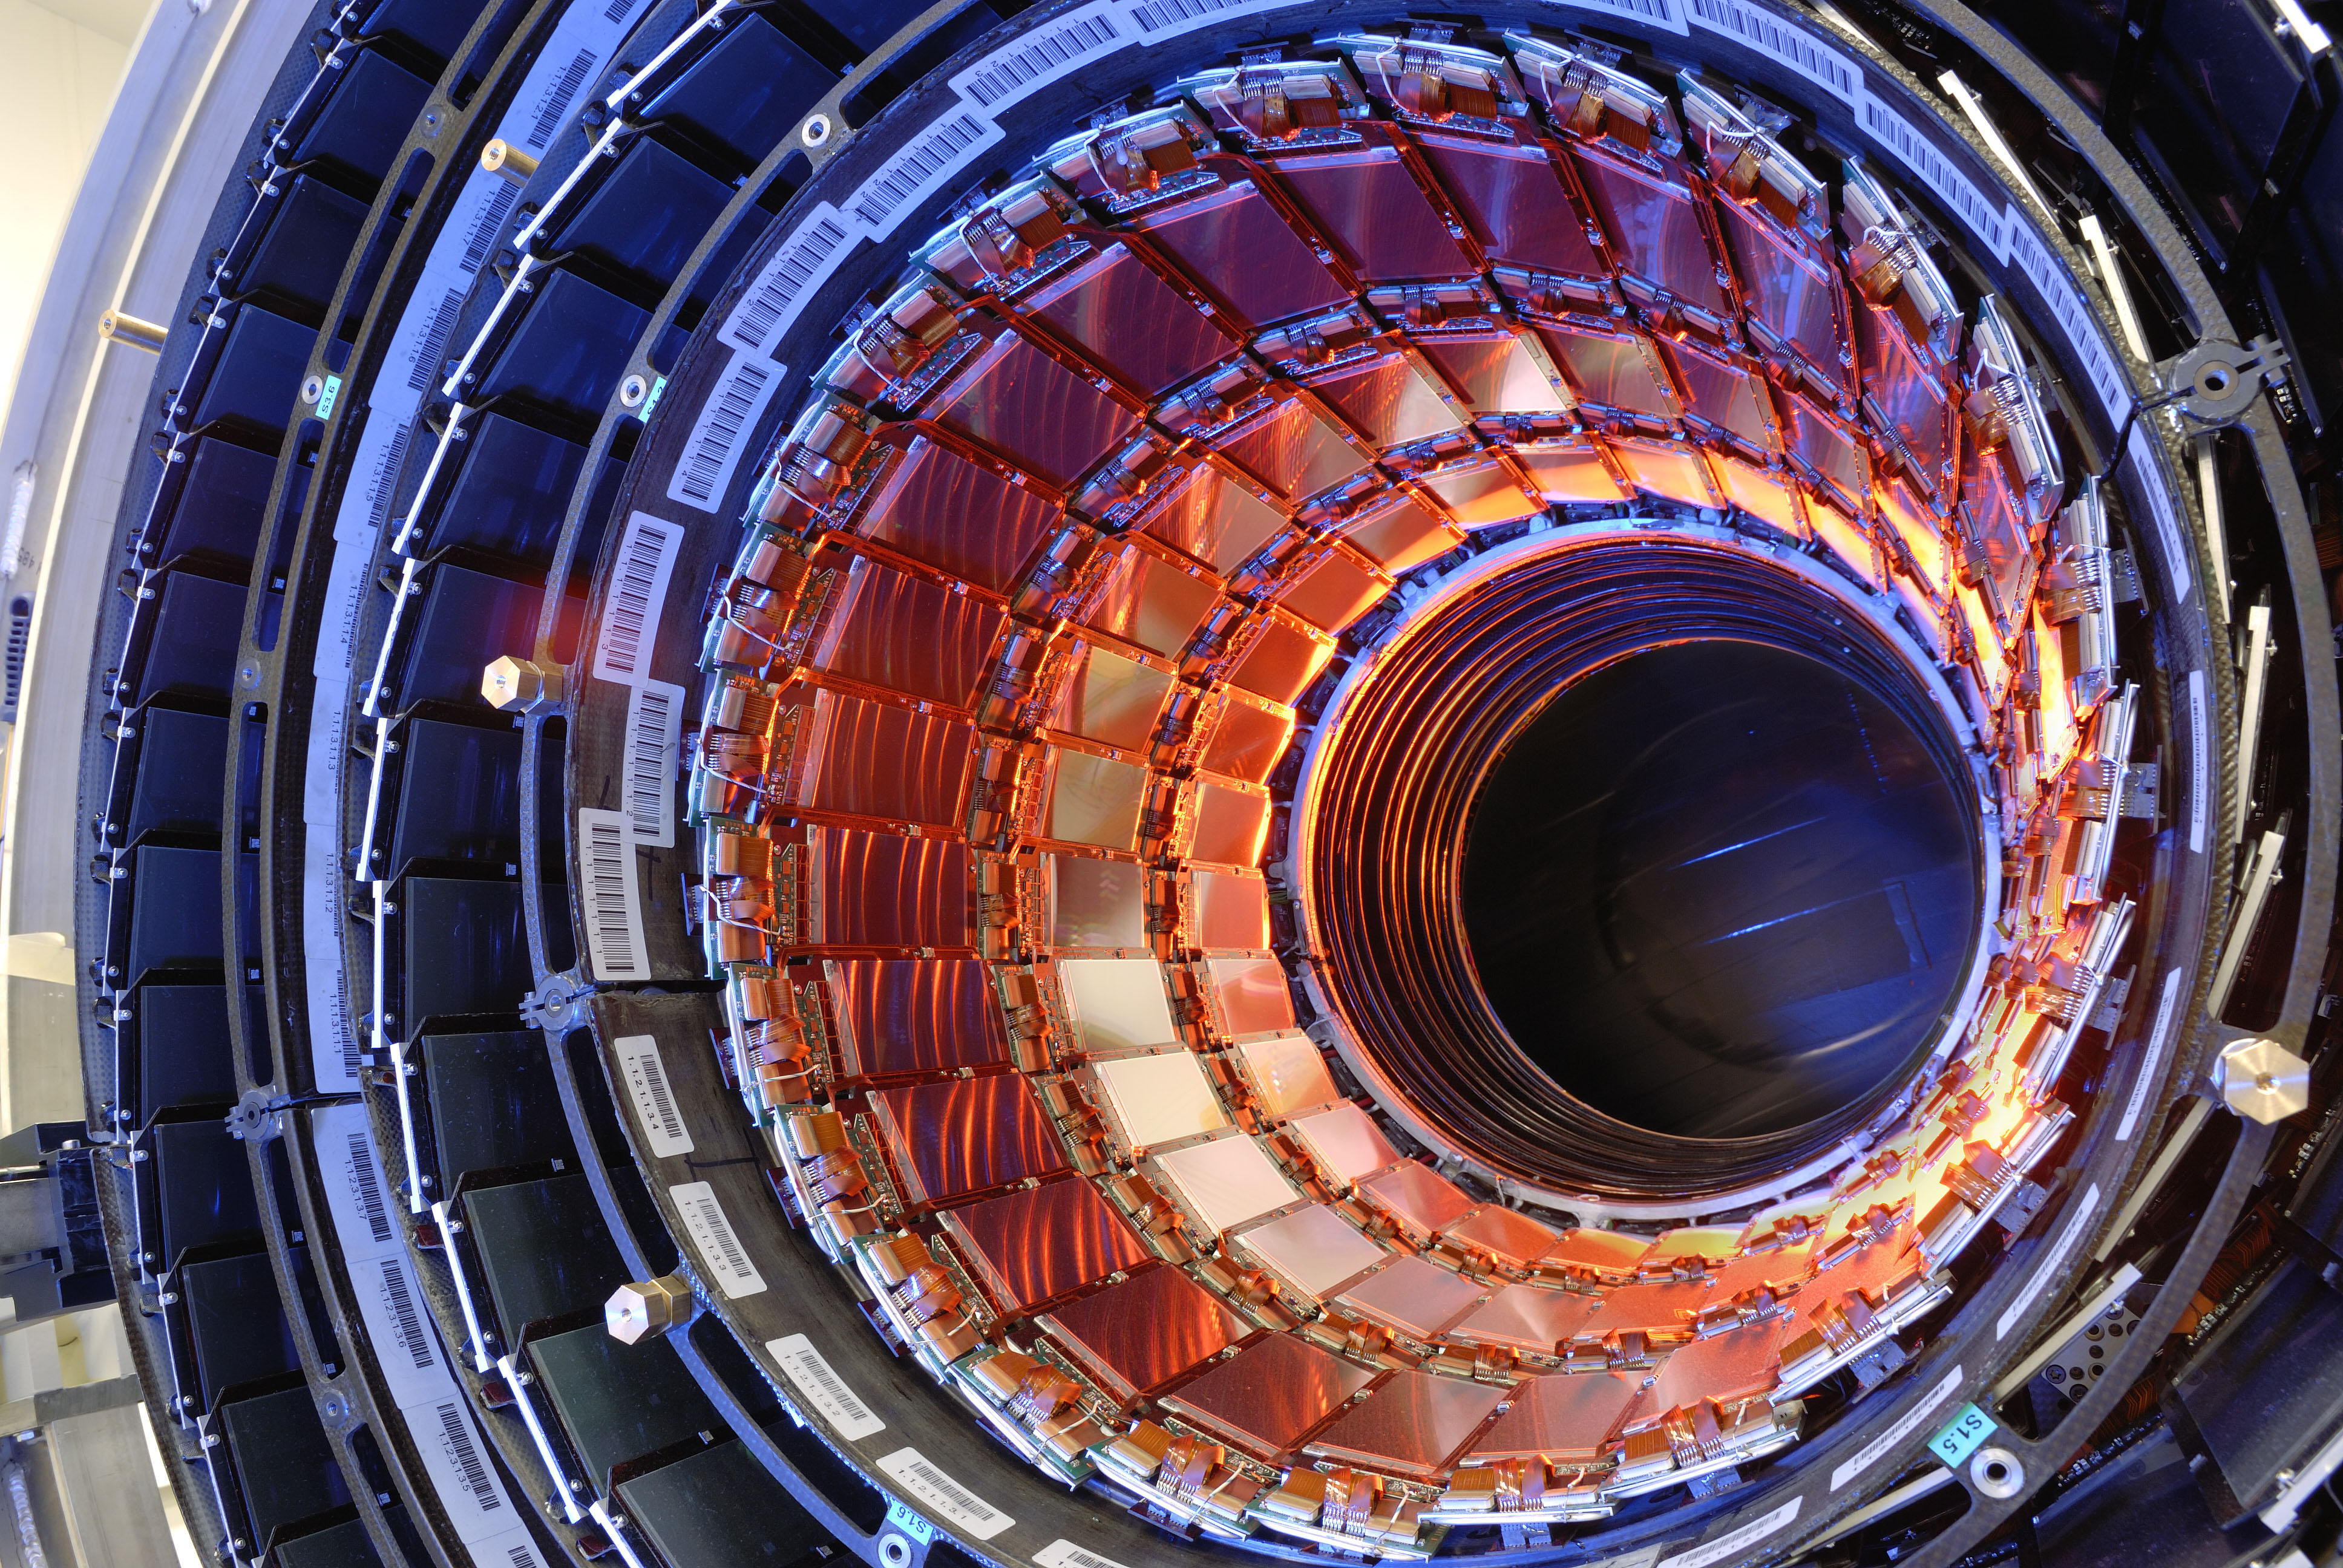
\includegraphics[width=0.70\linewidth]{Experiment/CMS/Image/Tracker/cms_track.jpg}}
  \hfil
  \subfigure[The position of silicon tracker on both sides of the IP ($z$ = 0\unit{cm}) \cite{Chatrchyan:2014fea}. 
	The pixel trackers are very close to the IP. For the strip tracker,
	there are tracker inner barrel (TIB), tracker outer barrel (TOB)
	in the barrel region, tracker endcap (TEC), and tracker inner disk (TID)
	in the transition region. The black (blue) lines correspond to single 
	(double) sided silicon strips. 
  \label{subfig:cms_track_pos}]
  {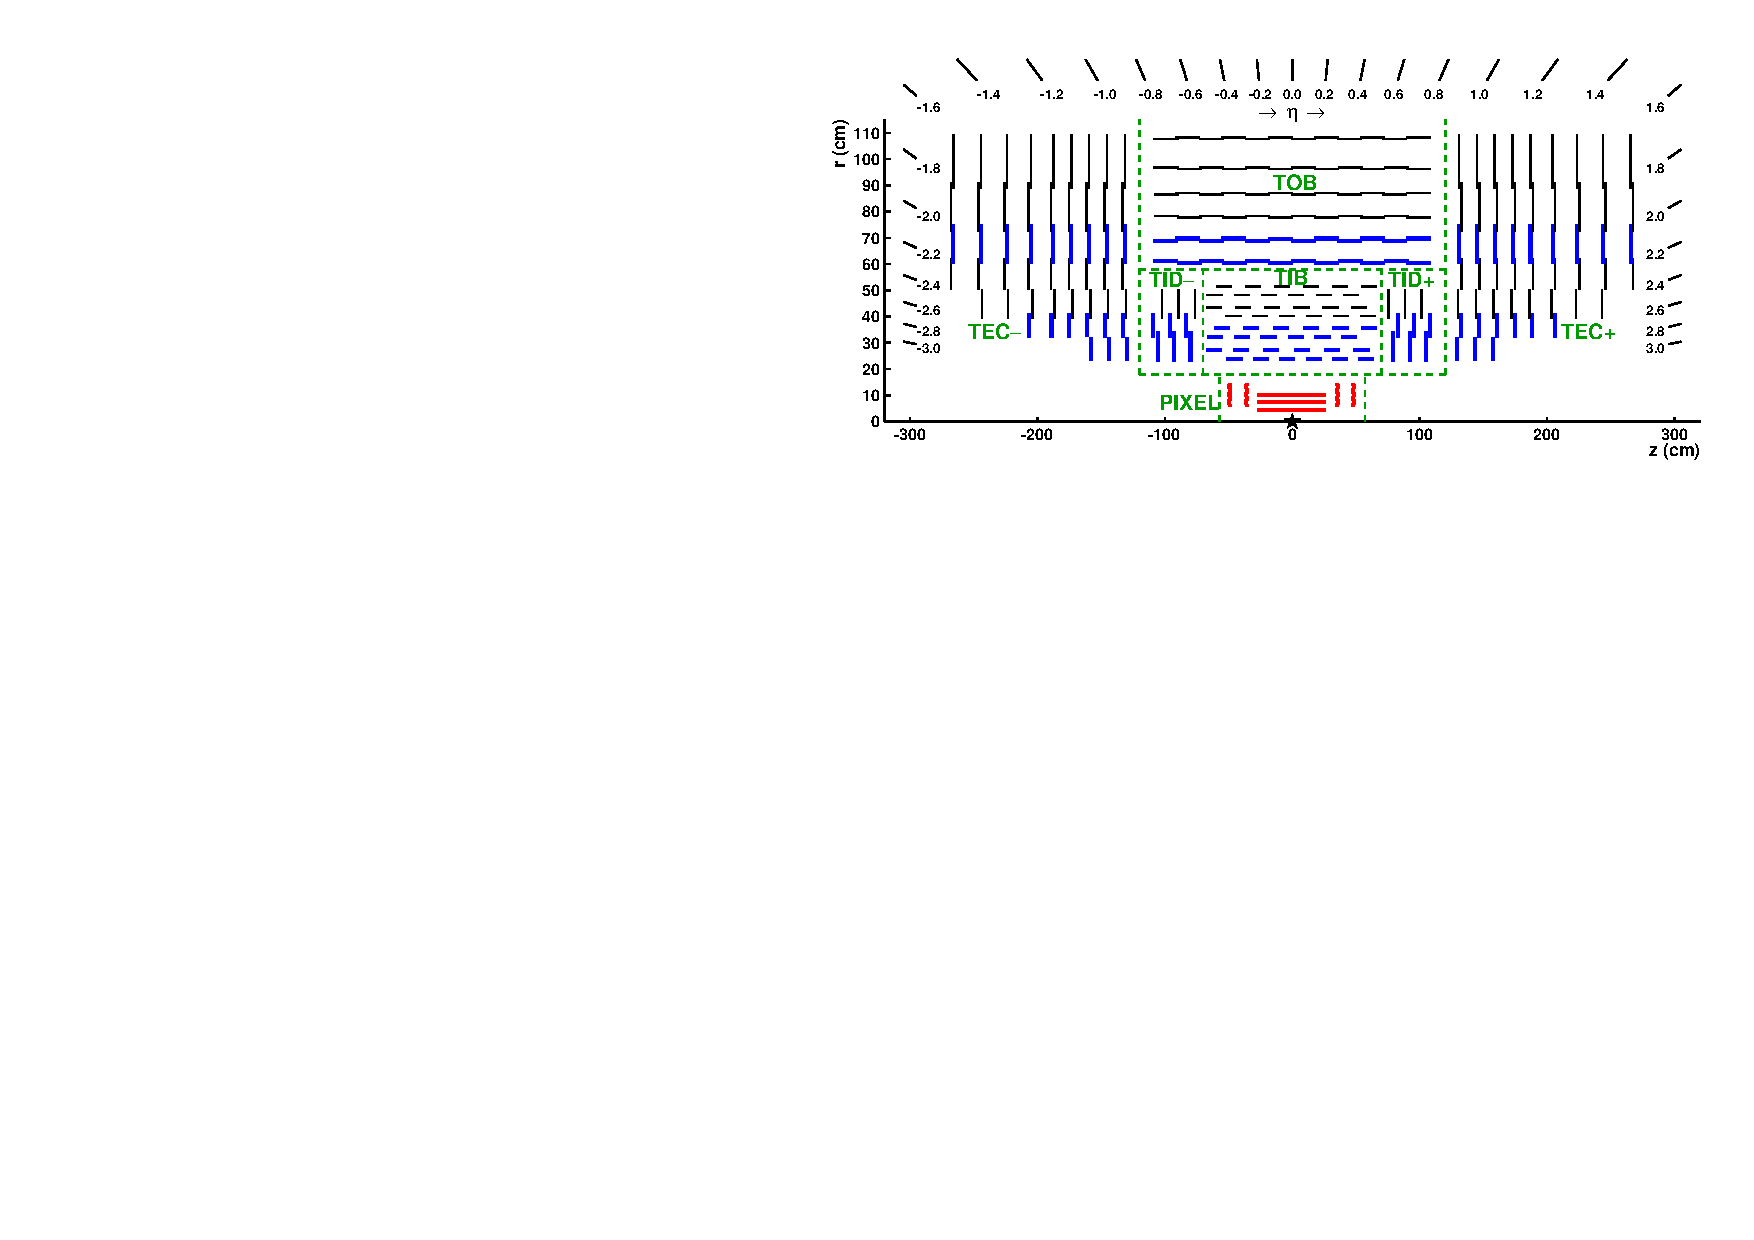
\includegraphics[width=0.90\linewidth]{Experiment/CMS/Image/Tracker/TrackerLayoutNew.pdf}}
  \caption{The silicon tracker of the CMS. The picture of one of trackers 
	inner barrel is shown in (a). The radial and $\eta$ position of the various
	parts of the pixel and strip tracker is shown in (b).}
  \label{fig:cms_tracker}
\end{figure}

The silicon detector is a reverse biased \rm{pn} junction, whose principle of operation 
is shown in Figure~\ref{fig:cms_diode}. Under the reverse 
bias voltage (80V), when a particle (for example, a minimum ionising particle) traverses 
through the bulk n-type region, several electron-hole pairs ( about 24,000) are created in 
the depletion region. The electrons, thus created, are attracted towards the $\rm p^+$ 
implant due to the applied electric field within very short time of about 10 ns.
The electrons collected at $\rm p^+$ implant are amplified and readout by the backend electronics.
\begin{figure}
  \begin{center}
	  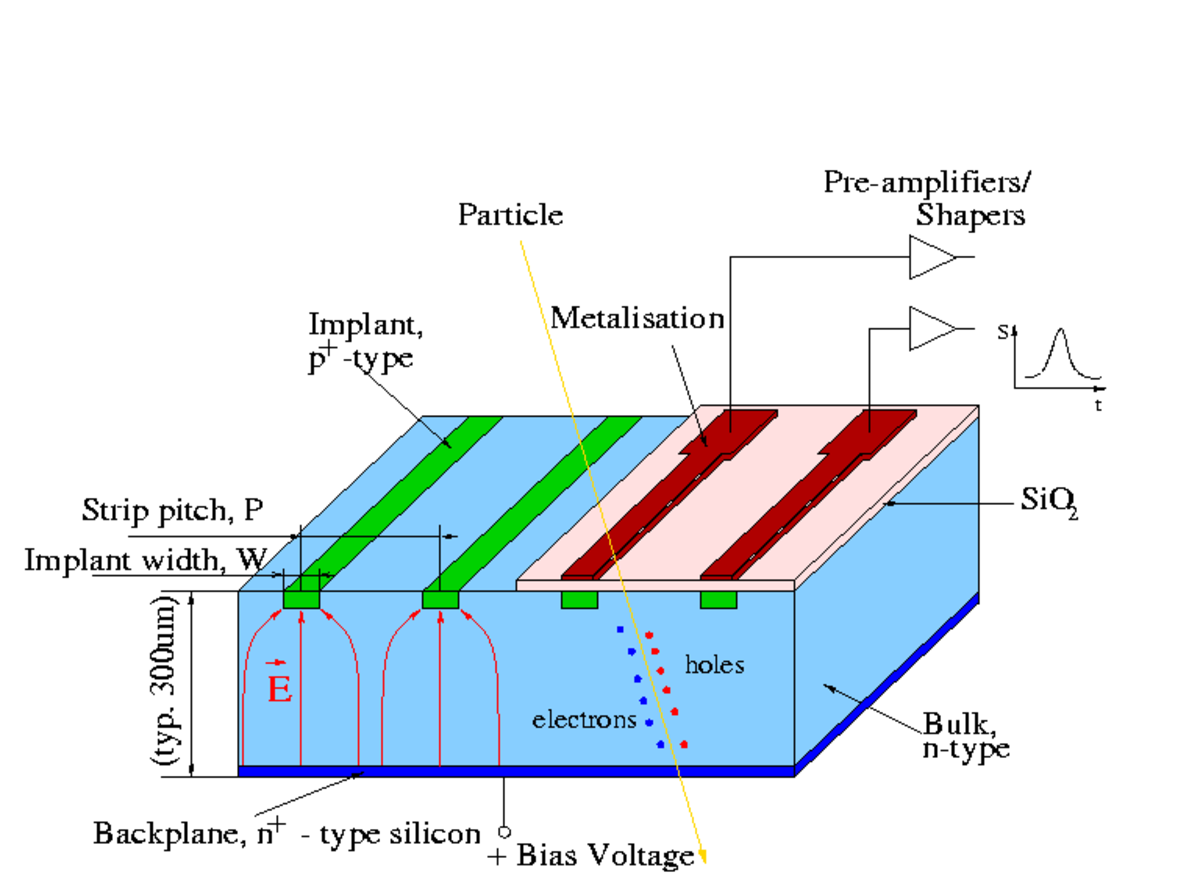
\includegraphics[width=0.75\linewidth]{Experiment/CMS/Image/Tracker/cms_diode.pdf}
  \caption{The principle of operation of a silicon detector \cite{Diode}. The green
	  strips are $\rm p^+$ -type of semiconductor where the electrons are 
	  attracted after being produced in the depletion region when a particle
	  passes through. The $\rm{SiO}_2$ layer along with metallic surface, on top of 
	  the green strips, provides conducting circuits for the electron. The 
	  amplifiers/shapers are used to amplify and shape the electron current.
	  The holes are attracted towards the $+ve$ bias voltage.}
  \label{fig:cms_diode}
  \end{center}
\end{figure}

As alluded earlier, the CMS silicon tracker is divided into two types:
\begin{itemize}[leftmargin=*]		
\item $\textbf{Pixel tracker}$:
	The innermost component of the tracker, the pixel detector occupies the central 
	region close to which the collision happens. It operates in a 
	high-radiation environment. The length of the pixel detector from 
	interaction point along the beam axis is 46.5\unit{cm}, while two endcaps are placed 
	at $z$ = 34.5 and 46.5\unit{cm} from both sides of the IP. The 3-layers of the detector
	are placed at r = 4.4, 7.3, and 10.2\unit{cm} in the barrel region as shown in 
	Figure~\ref{fig:cms_pixel}. 
	\begin{figure}
	  \centering
		\subfigure[Pixel layers \cite{Chatrchyan:2009aa} 
	  \label{subfig:cms_pixel}]
	  {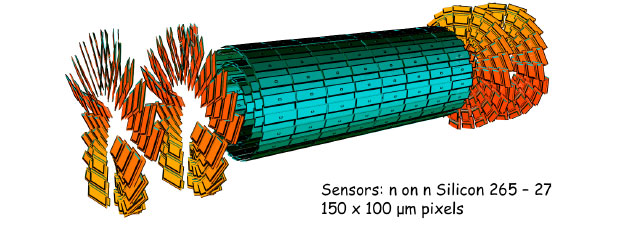
\includegraphics[width=0.50\linewidth]{Experiment/CMS/Image/Tracker/pixel.png}}
	  \hfil
	  \subfigure[Locations of pixel layers \cite{Veszpremi:2014exa}. 
	  \label{subfig:pixel_pos}]
	  {\includegraphics[width=0.40\linewidth]{Experiment/CMS/Image/Tracker/pixel2.png}}
	  \caption{The pixel detector of the CMS tracker. The location of pixel layers 
		in the barrel and endcap region is shown in (b).}
	  \label{fig:cms_pixel}
	\end{figure}
\item $\textbf{Strip tracker}$:
	The major part of the tracker is covered by the silicon strip detectors 
	as shown in Figure~\ref{fig:cms_tracker}. The length of strip detectors
	is 5.8\unit{m}, and diameter is 2.5\unit{m}. There are over 15000 modules covering 
	$0 \geq \eta \geq 2.5$. The charge generated, when a particle passes 
	through the strip detectors, is read and amplified from each micro-strip 
	as shown in Figure~\ref{fig:cms_diode}. 
\end{itemize}

The total thickness of tracker material in units of radiation length (it is a characteristic 
of a material defined as the distance traveled by an electron when it
loses $1/e$ of its energy due to the Bremsstrahlung radiation) and nuclear interaction length
(it is the mean distance a hadronic particle travels before undergoing an inelastic
nuclear interaction) is shown in Figure~\ref{fig:cms_track_budget}. In the direction
perpendicular to the $z$-axis ($\eta = 0$), the thickness is small ($t/X_0 \approx 0.4$).
That is, an electron produced at collision point can traverse in the $\eta = 0$ 
direction by losing only 14.7\% (0.4/2.718) of its initial energy. The thickness is 
maximum in the endcap region as shown in Figure~\ref{fig:cms_track_budget}.
\begin{figure}
  \centering
  \subfigure[Thickness in units of radiation length]
  {\includegraphics[width=0.49\linewidth]{Experiment/CMS/Image/Tracker/MaterialBudget_RadLengths.pdf}}
  \hfil
  \subfigure[Thickness in units of interaction length]
  {\includegraphics[width=0.49\linewidth]{Experiment/CMS/Image/Tracker/MaterialBudget_InteractionLengths.pdf}}
  \caption{Total thickness of the silicon tracker in units of radiation and interaction 
	lengths \cite{Chatrchyan:2014fea}. The thickness of supporting tube and beam 
	pipe is also shown.}
  \label{fig:cms_track_budget}
\end{figure}

The resolution is the parameter that characterizes how accurately a measurement
is performed. For example, if a detector \dq{measures} the momentum of a particle
to be 100 \GeV and the momentum \dq{resolution} is 5 \GeV then it implies that the 
\dq{actual} value of the momentum would be in the range of 95 to 105 \GeV. Hence lower the 
value of detector resolution, the more precise is the measurement. The absolute 
(relative) resolution of $\phi$ (\pt) of the silicon tracker as a function of $\eta$
is shown in Figure~\ref{fig:cms_track_reso_part} of muons, electrons, and charged
pions \cite{Chatrchyan:2014fea}. The $\eta$ and \pt resolution of all particles are 
better in the barrel region as compared to that in endcap regions. The resolution 
for muons is better as compared to electrons and charged pions in all regions. Also, 
the higher the \pt, better is the resolution for all charged particles. For \pt = 100 \GeV, 
the momentum resolution at $\eta$ = 0 is 2\%, 30\%, and 3\% for muons, electrons, and pions 
respectively.
The silicon tracker is essential for the reconstruction of trajectories of charged particles. 
Being very close to the collision point, these are also useful for high level triggering as discussed 
in Section~\ref{ss:secTrig}. 

\begin{figure}
  \centering
  \subfigure[]
  {\includegraphics[width=0.40\linewidth]{Experiment/CMS/Image/Tracker/mu_resolutionPhiVsEta.pdf}}
  \subfigure[]
  {\includegraphics[width=0.40\linewidth]{Experiment/CMS/Image/Tracker/mu_resolutionPtVsEta.pdf}}
  \vfil
  \subfigure[]
  {\includegraphics[width=0.40\linewidth]{Experiment/CMS/Image/Tracker/ele_resolutionPhiVsEta.pdf}}
  \subfigure[]
  {\includegraphics[width=0.40\linewidth]{Experiment/CMS/Image/Tracker/ele_resolutionPtVsEta.pdf}}
  \vfil
  \subfigure[]
  {\includegraphics[width=0.40\linewidth]{Experiment/CMS/Image/Tracker/pi_resolutionPhiVsEta.pdf}}
  \subfigure[]
  {\includegraphics[width=0.40\linewidth]{Experiment/CMS/Image/Tracker/pi_resolutionPtVsEta.pdf}}
  \caption{The absolute resolution of $\phi$ and relative resolution of \pt measurement
  of muons, electrons, and charged pions from the silicon tracker as function of 
  $\eta$ \cite{Chatrchyan:2014fea}. Other resolution such as $d_0, z_0$, 
  and $\cot\theta$ are given in Reference~\cite{Chatrchyan:2014fea}. The open (solid) markers 
  correspond to the half-width for 90\% (68\%) intervals \cite{Chatrchyan:2014fea}.}
  \label{fig:cms_track_reso_part}
\end{figure}

\section{Electromagnetic calorimeter}
The electromagnetic calorimeter (ECAL) is used to measure the energy deposited by 
electrons, photons, and jets. Due to the high collision rate (collisions happen after 
every 25\unit{ns}), the ECAL has to be very fast and responsive. In view of this, most 
part of ECAL is made of lead tungstate (PbWO$_4$) crystals which are birefringent,
tetragonal, and radiation-hard \cite{PbWO4}. A small part is made of the Pb absorber
(placed in the endcap region, primarily to differentiate events coming from 
$H\rightarrow \gamma\gamma$ and $\pi^0 \rightarrow \gamma\gamma$). A typical PbWO$_4$ 
crystal is shown in Figure~\ref{subfig:cms_ecal_PbWO4}. The volume of a PbWO$_4$ crystal is 
roughly equal to the volume of a coffee cup, and the weight of each crystal is 1.5\unit{kg} (the 
density is 8.3\unit{$\rm g/\rm {cm}^3$}). 
The PbWO$_4$ crystals are grouped in to form modules, and the modules are grouped to form 
super-modules. These super-modules are placed in barrel and endcap region of the ECAL as 
shown in Figure~\ref{subfig:cms_ecal_pos}. The ECAL is made up of 76,000 lead tungstate 
crystals (61,200 in the barrel and 14,800 in the endcap region).
%Fig\pdfcomment[author={FIG COURTESY}]{Ecal-pic: https://inspirehep.net/record/1251416/plots, crystal-pic:http://cms.web.cern.ch/news/electromagnetic-calorimeter}}
\begin{figure}
  \centering
	\subfigure[PbWO$_4$ crystal \cite{Collaboration_2008_CMS}
	 \label{subfig:cms_ecal_PbWO4}]
	 {\includegraphics[width=0.40\linewidth]{Experiment/CMS/Image/ECAL/ecal2.jpg}}
	 \hfil
	\subfigure[Components of the ECAL \cite{Collaboration_2008_CMS}
 	\label{subfig:cms_ecal_pos}]
 	{\includegraphics[width=0.40\linewidth]{Experiment/CMS/Image/ECAL/ecal.png}}
 	\caption{(a) A PbWO$_4$ scintillating crystal. (b) The various components of the 
	electromagnetic calorimeter in the barrel and endcap regions.}
 	\label{fig:cms_ecal}
\end{figure}

When a particle passes through the PbWO$_4$ crystals, photons are produced by the
scintillating process. The PbWO$_4$ are inorganic scintillator doped with impurities.
Other inorganic scintillators are alkali halide (NaI+TI, CsI+Na), 
Cerium-activated fast inorganics (LaBr$_3$), etc. Pure crystals such as NaI (octahedral) 
don't produce visible photons so impurities such as TI (activators) are added which 
create special sites in the lattice as shown in Figure~\ref{fig:cms_sinti}. When a
particle passes through the crystal it creates electron-hole pairs. The electrons are 
excited to the conduction band whereas the holes ionise the impurity atoms. The excited 
electron recombines the ionised impurity atoms creating its own excited configurations.
The impurity excited configuration de-excites to the ground state by emitting photons. 
\begin{figure}
  \centering
  {\includegraphics[width=1.0\linewidth]{Experiment/CMS/Image/ECAL/Scintillation.pdf}}
	\caption{The energy band structure in pure (impure) inorganic scintillator shown
	on left (right) side. The impurity creates intermediate excited states between
	the valence and conduction band. The photons are emitted when activator 
	de-excites.}
  \label{fig:cms_sinti}
\end{figure}

The photons thus produced are converted into an electrical signal by the 
photomultiplier tubes (PMTs) or avalanche photodiodes (APDs). The APDs in the
barrel and vacuum phototriodes (VPTs) are placed in the endcap region. The 
electrical signals are amplified and stored. The working principle of PMT is shown 
in Figure~\ref{subfig:cms_pmt}. The photons 
are absorbed on photocathodes. Due to the photoelectric effect, electrons are emitted, 
if the energy of incoming photons is more than $\approx$ 3\unit{eV}. The emitted electrons 
are directed towards the dynodes by an electric field. From the dynodes, the
secondary electrons are emitted with an efficiency (the ratio of number of secondary 
and primary electrons) of $\approx$ 6-8. These electrons are then directed towards 
other dynodes and the process continues. In the end, there are many electrons. 
A schematic diagram of APD is shown in Figure~\ref{subfig:sinti_apd}. When a photon enters 
the depletion region, electron-hole pairs are created. The created electron-holes start moving towards
the respective electrode due to large reverse bias voltage. While moving, they
create additional electron-hole pairs. The process continues producing an avalanche
multiplication.
\begin{figure}
  \centering
	\subfigure[Schematic diagram of photomultiplier tube \cite{pmt}
	 \label{subfig:cms_pmt}]
	 {\includegraphics[width=0.50\linewidth]{Experiment/CMS/Image/ECAL/pmt.jpg}}
	 \hfil
	\subfigure[Principle of operation of the avalanche photo-diode \cite{apd}
	 \label{subfig:sinti_apd}]
	 {\includegraphics[width=0.30\linewidth]{Experiment/CMS/Image/ECAL/apd.png}}
	 \caption{The schematic diagram of a circular and cylindrical PMT (a). 
	 The principle of operation of an APD is shown in (b).}
	 \label{fig:cms_pmt_apd}
\end{figure}

An electromagnetic pre-shower, as shown in Figure~\ref{subfig:cms_ecal_preS} is placed
in the endcap region at $z$ = 298.5\unit{cm} to distinguish photons coming from Higgs and pion.
The photons produced by the pion ($\pi^0$) are likely to be narrowly separated and
will be traveling in the forward direction. However, those coming from the Higgs 
are well separated and mostly in the transverse direction. Therefore, if
there is a photon in an event which was reconstructed using the preshower then
it most likely came from the $\pi$ decay and can be rejected for the study of
$H \rightarrow \gamma \gamma$ process.
The preshower has a diameter of 240\unit{cm} with a thickness of 20\unit{cm}. It 
has alternate layers of absorber and detectors on both sides of its center. 
Electromagnetic showers are produced from lead layers when a photon passes through it, 
which silicon sensors detect. The two layers are used to determine the position of the 
particles. 
\begin{figure}
  \centering
	\subfigure[Preshower disk 
  \label{subfig:cms_ecal_preS}]
  {\includegraphics[width=0.30\linewidth]{Experiment/CMS/Image/ECAL/ecal3.png}}
  \hfil
  \subfigure[Composition of preshower
  \label{subfig:sinti_ecal_preS_pos}]
  {\includegraphics[width=0.50\linewidth]{Experiment/CMS/Image/ECAL/ecal4.jpg}}
  \caption{ECAL preshower \cite{preS} placed in the endcap region at $z$ = 298.5\unit{cm}. The 
	preshower is made of alternate layers starting from the moderator, to 
	heating film to foam to cooling block to the absorber (Pb) to silicon
	detectors to the digital electronics. The width of the lead (Pb) absorber
	is not the same on both sides.}
  \label{fig:cms_ecal_pre}
\end{figure}

For a given energy \textit{E} (in \GeV), the energy resolution of ECAL is given by 
\cite{Chatrchyan:2013dga}
\begin{equation}
	\frac{\sigma_E}{E} = \frac{2.8\%}{\sqrt{E}} \oplus \frac{12.8\%}{E} \oplus 0.3\%
	\label{eq:cms_ecal_reso}
\end{equation}
where the terms in the quadrature sum correspond to the stochastic correction which accounts
for the energy deposited in the preshower and event-by-event fluctuations, the noise term
due to noise in backend electronics, and a constant term which takes into account
the non-uniformity of the detector and temperature gradient. From 
Equation (\ref{eq:cms_ecal_reso}), it is clear that the stochastic and noise term 
dominate at lower energies whereas the constant term becomes dominant at higher energies. 

The relative energy resolution as a function of $\eta$ of supercluster 
($ 3\times 3$ crystal) for electron and photon is shown in 
Figure~\ref{fig:cms_ecal_reso}. The relative resolution is shown in both barrel and
endcap region for $R_9 < 0.94$, $R_9 > 0.94$, where $R_9$ is a cluster shape parameter 
defined as $\rm{max}(E_{3\times 3})/E_{\rm{sc}}$. The $\rm{max}(E_{3\times 3})$ is the 
maximum energy deposited in a particular crystal out of 9 crystal, and $E_{\rm{sc}}$ is
the energy deposited in the supercluster, that is, the sum of energy deposited in all 9
crystals \cite{Chatrchyan:2013dga}. The relative energy resolution from observed data,
simulated MC, and smeared MC were determined 
at $\sqrt{s} = 7$ \TeV. The relative resolutions are better in the barrel as compared to 
the endcap region for $R_9 < 0.94$ as well as $R_9 > 0.94$ for electron and photon. From data, 
the minimum (maximum) resolution is about 1\% (5\%) for both electron and photon.

\begin{figure}
  \centering
  \subfigure[]
  {\includegraphics[width=0.39\linewidth]{Experiment/CMS/Image/ECAL/SCe_EtaR9calib_regression_EB_ER_ir9_0.pdf}}
  \subfigure[]
  {\includegraphics[width=0.39\linewidth]{Experiment/CMS/Image/ECAL/SCphoton_Reso_EB_ER_ir9_0.pdf}}
  \vfil
  \subfigure[]
  {\includegraphics[width=0.39\linewidth]{Experiment/CMS/Image/ECAL/SCe_EtaR9calib_regression_EB_ER_ir9_1.pdf}}
  \subfigure[]
  {\includegraphics[width=0.39\linewidth]{Experiment/CMS/Image/ECAL/SCphoton_Reso_EB_ER_ir9_1.pdf}}
  \vfil
  \subfigure[]
  {\includegraphics[width=0.39\linewidth]{Experiment/CMS/Image/ECAL/SCe_EtaR9calib_regression_EE_ER_ir9_0.pdf}}
  \subfigure[]
  {\includegraphics[width=0.39\linewidth]{Experiment/CMS/Image/ECAL/SCphoton_Reso_EE_ER_ir9_0.pdf}}
  \vfil
  \subfigure[]
  {\includegraphics[width=0.39\linewidth]{Experiment/CMS/Image/ECAL/SCe_EtaR9calib_regression_EE_ER_ir9_1.pdf}}
  \subfigure[]
  {\includegraphics[width=0.39\linewidth]{Experiment/CMS/Image/ECAL/SCphoton_Reso_EE_ER_ir9_1.pdf}}
	\caption{The relative energy resolution of electron and photon as a function
	of supercluster $\eta$ in the barrel and endcap region of the ECAL 
	\cite{Chatrchyan:2013dga}.}
  \label{fig:cms_ecal_reso}
\end{figure}


\section{\rm{H}adron calorimeter}
The hadron calorimeter (HCAL) of the CMS experiment is used to measure the 
energy deposited
by hadrons (protons, pions, neutrons, kaons, etc). It is also useful
in estimating the missing transverse energy (as described in Section~\ref{s:secMET}) 
which is attributed to the neutrinos and unknown particles such as the dark 
matter. The HCAL is made of alternating layers of absorbers and plastic scintillators.
The absorber is made of brasses and steels whereas the scintillators are made
of Bicron-BC408 and Kuraray-SCSN81. When a particle passes through the 
absorber, it produces hadronic showers (a cascade of secondary particles). The 
secondary particles of the shower interact with the scintillating material
producing photons. The photons are converted into an electronic signal by hybrid
photodiodes (HPDs). The HCAL is made up of 36 barrel, 36 endcap wedges 
(weight of 1 wedge = 26 tonnes), 70000 tiles, and contains over 400 
optical decoder units which take light to the HPDs.
\begin{figure}
  \centering
  \subfigure[A prototype of HCAL barrel
  \label{subfig:cms_hcal1}]
  {\includegraphics[width=0.31\linewidth]{Experiment/CMS/Image/HCAL/hcal1.jpg}}
  \hfil
  \subfigure[The actual HCAL endcap
  \label{subfig:sinti_hcal2}]
  {\includegraphics[width=0.55\linewidth]{Experiment/CMS/Image/HCAL/hcal2.jpg}}
	\caption{The CMS hadron calorimeter \cite{Collaboration_2008_CMS}. A prototype of 
	HCAL barrel is shown in silver color in (a). The actual endcap part of the HCAL 
	is shown in (b).}
  \label{fig:cms_hcal}
\end{figure}

Plastic (organic) scintillators are used in HCAL, unlike the inorganic scintillators 
of the ECAL. The organic scintillators have a wide range of varieties such as a
pure organic crystal (anthracene $\rm C_{14}\rm H_{10}$), organic liquids 
(p-terphenyl $\rm C_{18}\rm H_{14}$), and a plastic scintillator (polyethylene 
naphthalate). The typical gap between the electronic (vibrational) energy 
levels is 3-4\unit{eV} (0.15\unit{eV}). The scintillation mechanism in an organic scintillator
is shown in Figure~\ref{fig:cms_org_sinti}. At room temperature, all 
molecules having an energy about 0.025 eV are in the singlet ground state
($S_{00}$). When a particle passes through the scintillator, it transfers part of its 
kinetic energy to the molecules exciting them to higher states. The 
de-excitations from $S_2 \rightarrow S_1$ and $S_3 \rightarrow S_1$ are radiationless transitions.
That is, a photon is not produced in such a transition. However, as a result of 
these transitions, the population at $S_1$ increases considerably. The 
transitions from $S_1$ to lower energy states result in the emission of 
photons. There are two types of such transitions. The first is from 
$S_1 \rightarrow S_0$ called fluorescence, and the second is 
$S_1 \rightarrow T_1 \rightarrow S_0$ called phosphorescence. The light 
produced from such transitions is converted into electric signals by HPDs. 
The HPD uses photomultiplier-cum-semiconductor photodiode principle.  
\begin{figure}
  \begin{center}
  \includegraphics[width=0.5\linewidth]{Experiment/CMS/Image/HCAL/organic_sinti.pdf}
	\caption{The energy levels of a molecule of an organic scintillator 
	  \cite{wiki:orgSinti}. The ground state is $S_0$ followed by vibration
	  sublevels ($S_{01}, S_{02}$ etc). The $S_{1, 2, 3}$ are the excited 
	  singlet energy levels. In between the singlet, there are triplet energy 
	  levels shown as $T_{1, 2, 3}$. The fluorescence (phosphorescence) occurs
	  when there is a transition from $S_1 (T_1) \rightarrow S_{03, 02, 01, 00}$.}
  \label{fig:cms_org_sinti}
  \end{center}
\end{figure}


The HCAL calorimeters are placed in the barrel and endcap regions as shown in
Figure~\ref{fig:cms_hcal_pos} along with its various components. 
\begin{figure}
  \begin{center}
  \includegraphics[width=0.75\linewidth]{Experiment/CMS/Image/HCAL/hcal.png}
	  \caption{The location of various components (HB, HO, HE, and HF) of 
	  the HCAL \cite{Isildak:2013kfa}.}
  \label{fig:cms_hcal_pos}
  \end{center}
\end{figure}
The hadron calorimeters are in the barrel (HB), endcap (HE), outer (HO), and 
forward (HF) region. The HO is placed outside of the magnetic solenoid acting
as a tail catcher. The HF is used to study jets in the forward region coming
from high radiations. More description of various components of the HCAL is given below:
\begin{itemize}[leftmargin=*]
  \item \textbf{Hadron Barrel}:
	The HB has a fine and uniform granularity in the $\eta-\phi$ plane, 
	for example, $\Delta\eta\times\Delta\phi = 0.087\times 0.087$.
	Due to high thickness, around 7-11 times of the interaction length,
	the HB stops almost all the hadrons passing through it.
  \item \textbf{Hadron Outer}:
	Even though all the hadrons are supposed to be stopped in the HB, there
	is a chance for high energetic hadrons to go outside the HB and magnetic
	solenoid. To measure the energy of hadronic showers from such hadrons,
	the HO is placed outside the magnet. The HO covers $|\eta| = 1.26$ range. 
  \item \textbf{Hadron Endcap}: The HE covers the $1.3\geq |\eta|\geq 3.0$
	region, with 14 additional calorimeter towers. Being close to the beam
	pipe, it is radiation hard. The response of the HE is regularly 
	calibrated during the data taking. The HB and HE overlap in the 
	1.305 $\geq |\eta| \geq 1.392$ region.
  \item \textbf{Hadron Forward}: The HF is located in the forward region
	in the range $1.3\geq |\eta| \geq 3.0$, and $z = \pm$ 11.2 m from the
	collision point. The length of the HF is 1.65 m, divided into 900 towers.
	The hadronization product of the beam remnants and jets with very high
	$\eta$ value are detected by the HF.
\end{itemize}

The energy resolution of the HCAL is given by
\begin{equation}
	\left(\frac{\sigma}{E}\right)^2 = \left(\frac{s}{\sqrt{E}}\right)^2 + c^2,
\end{equation}
where the energy of hadron ($E$) is measured in \GeV, the constant 
$s = (0.847)$\GeV$^{1/2}$ and $c = 0.074$ for all part of 
the HCAL except the HF. For the HF, $s = 1.98 $ \GeV $^{1/2}$ and $c = 0.09$.
The pion energy resolution from the HCAL is shown in Figure~\ref{fig:cms_hcal_reso}.
For low $E$, the resolution is poor, while for $E > 100$ \GeV, it lies in 5-10\%
range.
\begin{figure}
  \begin{center}
  \includegraphics[width=0.50\linewidth]{Experiment/CMS/Image/HCAL/cms_hcal_reso.pdf}
  \caption{The HCAL energy resolution as a function of pion energy measured using
	  hybrid photodiodes, and silicon photomultipliers with different pixel
	  density \cite{Mans:1481837}.}
  \label{fig:cms_hcal_reso}
  \end{center}
\end{figure}

\section{Magnet}
The magnet bends charged particles moving inside and
outside of it. Lower the momentum of a particle, the more it is bent and vice
versa. The weight of the magnet is 12,000 tonnes, being the largest superconducting
magnet ever built.
\begin{figure}
  \begin{center}
  \includegraphics[width=0.50\linewidth]{Experiment/CMS/Image/cmssol.jpg}
	  \caption{An artistic view of the CMS solenoid~\cite{cmsSol}. 
	  An aluminum alloy shell, with a thickness of 50\unit{mm}, is placed on the 
	  inner and outer surface of the solenoid and used as a cooling wall.
	  Outside the solenoid are the return iron yokes which hold the 
	  magnetic flux.}
  \label{fig:cms_sol}
  \end{center}
\end{figure}
There are three main parts of the magnet: a solenoid, a vacuum 
tank, and the return iron yoke. A brief description of each component is given below:
\begin{itemize}[leftmargin=*]
\item \textbf{Solenoid}:
	The solenoid is made of NbTi (Niobium Titanium) coils which 
	is an aluminum-stabilized and mechanically reinforced superconducting 
	material. The solenoid is formed by placing 5 modules side-by-side 
	along the $z$-axis. With the length of 2.5\unit{m}, each module has 4 internal 
	layers of winding, each with 109 turns. Therefore, the total length of 
	the solenoid is $5\times 2.5$\unit{m} $ = 12.5$\unit{m}, with $5\times 4 \times 109 = 
	2180$ turns. The diameter of the solenoid is 6\unit{m}. The magnetic field 
	inside the solenoid is given by
	\begin{equation}
		B = k\mu_0\times N\times I/L
	\end{equation}
	Where $k$ is the relative permeability. Therefore, with 
	\textit{k} = 0.90, $\mu_0 = 4\pi\times 10^{-7}$\unit{mT/A}, N = 2180, 
	I = 19.14\unit{kA}, and L = 12.5\unit{m}, the magnetic field inside the solenoid, 
	B = 3.8\unit{T}, which is 100,000 times stronger than the Earth's magnetic 
	field. Being a very high energy experiment, such a large magnetic 
	field is necessary for better tracking resolution.
\item \textbf{Vacuum tank}: A huge amount of heat is produced due to the 
	flow of such a large current. The energy contained inside the solenoid 
	is 2.7\unit{GJ} which is more than enough to melt 18 tonnes of gold. A 
	dedicated cooling system is placed to cool the solenoid down to 
	-268$^\circ$C.
\item \textbf{Return yoke}: With four layers in the barrel region, and six
	disks in the endcap region, a giant iron return yoke is placed outside 
	the solenoid to contain the magnetic flux. The iron yokes in the barrel 
	region are shown in Figure~\ref{fig:cms_sol}. Total weight of the
	iron yoke is 10000 tonnes.
\end{itemize}

The longitudinal and transverse component of the magnetic field produced from 
the solenoid is shown in Figure~\ref{fig:cms_mag}. The longitudinal component
is the strongest compared to the transverse component. The transverse one
 is everywhere zero except at the endcap in the region 6\unit{m} $<z<$ 10\unit{m}. 
The magnetic field of the longitudinal component is 3.8\unit{T} inside the solenoid,
and about 2\unit{T} inside the return iron yoke. Further, the longitudinal component
inside and outside the solenoid is in the opposite direction. By virtue of this property, 
the charged particles are bent in the opposite direction.
\begin{figure}
  \centering
  \subfigure[Longitudinal component of the magnetic field
  \label{subfig:cms_magl}]
  {\includegraphics[width=0.50\linewidth]{Experiment/CMS/Image/magl.png}}
  \hfil
  \subfigure[Transverse component of the magnetic field
  \label{subfig:sinti_magt}]
  {\includegraphics[width=0.50\linewidth]{Experiment/CMS/Image/magt.png}}
	\caption{Component of the magnetic field inside CMS~\cite{Lenzi:2013xpa}.}
  \label{fig:cms_mag}
\end{figure}


\section{Muon chambers}
\label{fig1:cms_muon2}
%Fig\pdfcomment[author={FIG COURTESY}]{http://cms.web.cern.ch/news/muon-drift-tubes}}
Detection of muons was the primary physics motive for the CMS experiment. Being
a minimum ionizing particle, the muon traverses most part of CMS without
losing much energy in the calorimeters. Except for the muons, other particles
produced in the collision are stopped either in ECAL or HCAL. In view of this,
muon chambers are placed at the outermost side of CMS where only muons are
supposed to be detected. The muon chambers have a different configuration in the
barrel and endcap regions. When a muon passes through the muon chambers, filled
with gases, atomic electrons are knocked out. Subsequently, the current corresponding
to these electrons is amplified and stored. As shown in Figure~\ref{fig:cms_mu},
the CMS experiment has the following three types of the muon chambers: drift tubes (DTs),
cathode strip chambers (CSCs), and resistive plate chambers (RPCs). The momentum resolution of 
the muon detector is 10\% (20\%) in the barrel (endcap) region for a muon with 
\pt = 40 \GeV. Various properties and parameters of the muon subsystem are listed in 
Table~\ref{tab:muChamberParam}. A brief description of these subsystems is given below.
\begin{figure}
\centering
\includegraphics[width=0.75\linewidth]{Experiment/CMS/Image/mu2.png}
\caption{Location of the various sub-detectors of the CMS 
	\cite{Sirunyan:2018fpa}. The DTs and CSCs are placed in barrel and 
	endcap regions. The RPCs are placed in both regions. The muon chamber
	in the barrel region is formed by placing three \dq{wheels} side-by-side
	along the $z$-axis whereas in the endcap regions different segments
	of RPC and CSC are placed along the radial direction.}
\label{fig:cms_mu}
\end{figure}
\begin{table}
   \caption{Various properties and parameters of the CMS muon subsystems 
	\cite{Sirunyan:2018fpa}.}
   \centering
   \begin{tabular}{cccc}
     \hline
     \hline
     Muon subsystem                &    DT                               &    CSC                  & RPC              \\
     \hline
     \hline
     $|\eta|$ coverage         & 0.0--1.2                            & 0.9--2.4                & 0.0--1.9         \\
     Number of stations            & 4                                   & 4                       & 4                \\
     Number of chambers            & 250                                 & 540                     & Barrel: 480      \\
                                   &                                     &                         & Endcap: 576      \\
     Number of layers per chamber      & \textit{R}-$\phi$: 8; \textit{z}: 4 & 6                       & 2 in RB1 and RB2 \\
                                   &                                     &                         & 1 elsewhere      \\
     Number of readout channels    & 172000                             & Strips: 266112         & Barrel: 68136   \\
                                   &                                     & Anode channels: 210 816 & Endcap: 55296   \\
     Percentage of active channels &   98.4\%                            &   99.0\%                &  98.3\%          \\
     \hline
   \end{tabular}
   \label{tab:muChamberParam}
 \end{table}

\begin{itemize}[leftmargin=*]
\item \textbf{Drift tube}: The DTs are placed in the barrel region. 
A schematic diagram of a DT is shown in Figure~\ref{fig:cms_dt}, where the 
red dots are the aluminum wires pointing into the page. The region between the wires 
are filled 85\% with Argon (Ar) and 15\% with $\rm{CO}_2$ gases. When a muon passes through 
the DTs, atomic electrons are knocked-out of the gases. The anode wires attract electrons
towards themselves. The distance traveled by electrons up to the anode wire is shown
by horizontal arrows. The information about the length of such arrows gives direction
in which the muon could have traversed inside the DTs, which give the $z$ and $\phi$ 
coordinates of the muon.
\begin{figure}
\centering
\includegraphics[width=0.50\linewidth]{Experiment/CMS/Image/DT.png}
\caption{Schematic view of one of the DTs of the muon chamber \cite{Collaboration_2008_CMS}. 
	The red dots are the aluminum wires pointing into the page, the red arrow is the
	direction of an incoming muon, and the horizontal blue lines are the 
	distance traveled by secondary electrons.}
\label{fig:cms_dt}
\end{figure}

\item \textbf{Cathode strip chamber}: A schematic diagram of the cathode strip
	chamber is shown in Figure~\ref{fig:cms_csc}. The CSC is placed in the
	endcap region where particle multiplicity is very high. It consists
	of anode wires of gold-plated tungsten and cathode strips made of copper. 
	The wires and strips are placed perpendicular to each other. A 
	mixture of different gases consisting of 50\% CO$_2$, 40\% Ar, and 10\% 
	CF$_4$ is filled between anode and cathode. When muon passes
	through the CSC, atomic electrons are knocked out of the gasses and attracted
	towards the anode wires. Whereas the ions are attracted towards the cathode
	strips. Therefore, two coordinates is determined from the CSC,
	unlike the DT where only one coordinate is determined. 
\begin{figure}
\centering
\includegraphics[width=0.50\linewidth]{Experiment/CMS/Image/CSC.png}
\caption{Schematic view of one of the cathode strip chambers~\cite{Collaboration_2008_CMS}. 
	The wires shown in red and cathode strips shown in cyan are placed perpendicular to each
	other.}
\label{fig:cms_csc}
\end{figure}

\item \textbf{Resistive plate chamber}: The response from the RPC is very
	fast, hence, it helps in quick triggering (see Section~\ref{ss:secTrig}).
	The time resolution of the RPC is 3\unit{ns}.
	A schematic diagram of one of the RPCs is shown in Figure~\ref{fig:cms_rpc}.
	There are two resistive plates: one acts as the anode and the other as the cathode.
	Only the anode plate is transparent to the secondary electrons.
	The region between the plates is filled with a mixture of gases (95.2\% 
	C$_2$H$_2$F$_4$, 4.5\% i-C$_4$H$_{10}$,	and 0.3\% SF$_6$). When a muon 
	passes through the gases, atomic electrons are knocked out. These electrons are 
	picked up by anode strips placed above the anode plate. The momentum of a 
	muon is measured from the hit pattern in the strips. The muon information is 
	conveyed to the global muon trigger (see Section~\ref{ss:secTrig}). 
\begin{figure}
\centering
\includegraphics[width=0.65\linewidth]{Experiment/CMS/Image/RPC.pdf}
\caption{Schematic diagram of one of the RPCs. The cathode (bottom red plate) and 
	anode (top red plate) is separated by a separator (shown in gray). The
	region between the two plates is filled with gas. The anode is
	transparent to the secondary electrons. The orange strips (above anode)
	picks the secondary electrons. The high voltage aluminum foil is placed
	at the bottom. This figure is adopted from ~\cite{Collaboration_2008_CMS}.}
\label{fig:cms_rpc}
\end{figure}
\end{itemize}



\section{The trigger}
\label{ss:secTrig}
At the LHC, the proton beams are made to collide after 25\unit{ns}. Due to such a high
collision rate a huge number of events, roughly 40 million, are produced at
every second. Storing all these events would require many petta bytes
(1\unit{PB} = 1000000\unit{GB}) of computer memory, which is practically not possible as the
collision happens over a large period of time (many months). Even if somehow one 
can get around this challenge, most of the events are produced from soft collision 
and contain no interesting physics process. To filter events which are of physics 
interest, a two-tier trigger system is deployed at the CMS experiment. The first is 
called Level-1 (L1) trigger which is based on hardware (by collecting information from 
various sub-detectors) and the second is called High Level Trigger (HLT) which 
is based on software algorithms. The event rate after passing through these 
triggers are shown in Table~\ref{tab:trigRate}. After applying the HLT, the 
event rate is reduced to 200\unit{Hz} which requires about 200\unit{MB} of computer memory. 
A brief description of the L1 and HLT triggers are given in this thesis. A detailed 
description of these can be found in Reference~\cite{Khachatryan:2016bia}.
\begin{table}
\caption{\label{tab:trigRate} Event rate after applying level-1 and high-level
	triggers.}
\begin{centering}
\begin{tabular}{cccc}
\hline
\hline
\noalign{\vskip 0.1cm}
	Input event rate & Trigger & Type & Output event rate 
\tabularnewline
\hline
\hline
\noalign{\vskip 0.1cm}
	40\unit{MHz} & L1   & Hardware & 100\unit{KHz} \tabularnewline
\noalign{\vskip 0.1cm}
	100\unit{KHz} & HLT & Software & 200\unit{Hz} \tabularnewline
\hline
\end{tabular}
\par\end{centering}
\end{table}


\begin{itemize} [leftmargin=*]
\item \textbf{Level-1 Trigger}: L1 is also called online trigger as 
events are triggered during the data taking. The L1 trigger is 
required to be very fast with a latency of 4\unit{$\mu$s}. The decision to either 
keep or reject events by this trigger is based on a set of information 
provided by various sub-detectors as shown in Figure~\ref{fig:L1Trig}.
Over 8000 towers of the calorimeters (ECAL and HCAL) send transverse energies
and quality flags to the regional calorimeter trigger (RCT). These pieces of
information are processed in parallel by the RCT. The $e/\gamma$ candidates along 
with $E_{T}$ sums based on $4\times 4$ towers are sent by RCT to the global calorimeter
trigger (GCT). The GCT finds central-jets, forward-jets, tau-jets, and missing transverse energy.
The decision based on the findings of GCT is conveyed to the global trigger (GT) 
whether to keep an event or not. The other decision conveyed to the GT comes 
from the global muon trigger (GMT). The GMT takes input from different muon chambers.
The hits from RPC is sent to the pattern comparator (PC) which finds muon 
candidates. The information about the number of muon candidates from the PC is 
shared with the GMT. The front-end trigger electronics identify segments from 
the hits in CSC and DT. These segments are sent to the regional track finder (TF).
In the TF, the PC comparator identifies muon candidates and measures momentum 
from the bending of tracks due to the magnetic field. The muon candidates with the
corresponding momentum from the TF are shared with GMT. The GMT decides whether
an event is worth keeping from muon's point of view. Finally, the collective
decision from the GCT and GMT is passed to the global trigger which takes
the final call. The decision of the GT is conveyed to the data acquisition system 
(DAQ) which stores data from sub-detectors such as tracker (TRK), ECAL, HCAL, and muon 
chambers. If the event is going to be rejected by the GT then the DAQ does not 
store corresponding data from the sub-detectors.
\begin{figure}
  \begin{center}
  \includegraphics[width=0.70\linewidth]{Experiment/CMS/Image/L1Trig.pdf}
  \caption{Workflow of decisions for the Level-1 trigger \cite{Khachatryan:2016bia}.}
  \label{fig:L1Trig}
  \end{center}
\end{figure}

\item \textbf{High Level Trigger}: After applying L1 trigger, the filtered events
are passed as input to the HLT. The L1 bits available in the event serve
as the seed for HLT. The decision to reject or keep an event from the HLT
is taken based on whether an event has a reasonable number of physics objects
such as electrons, muons, and jets  with transverse momentum above some
threshold. In order to reconstruct these physics objects, a set of dedicated
software algorithms is run for every event. During the run, the input from one 
step is passed to the subsequent steps. For every event, the HLT decision is 
stored in the form of programming strings also called trigger paths. 

The HLTs are applied to select events enriched
with desired physics objects. Depending on the topology of analysis, an 
event is selected if the corresponding trigger path is available in that 
event. In this thesis, we have 1 lepton, at least 4 jets, and neutrino in the 
final state. Therefore, an event is selected if it has a trigger 
path of \verb|HLT_IsoMu24*| and \verb|HLT_IsoTkMu24*| with logical \verb|OR| 
for the muon channel, and \verb|HLT_Ele27_WPTight_Gsf| for the electron 
channel. Having these muon trigger paths in the event ensures that there is at least one 
isolated muon with \pt more than 24 \GeV (see Section~\ref{s:muReco}) whereas
the electron trigger path implies the presence of at least one electron with \pt 
more than 27 \GeV with tight working point (WP) reconstructed with Gaussian sum 
filter algorithm (see Section~\ref{s:eleReco}). The efficiency of these triggers depends on 
\pt and $\eta$ of the lepton. For lower \pt, the efficiency is very poor and has 
a sudden increase at a particular value. That sudden increase is called trigger 
turn-on and the leptons are required to have a \pt greater than that at the turn-on.

The muon and electron trigger efficiency as a function of \pt is shown 
in Figure~\ref{fig:trigEff}. The trigger turn-on for muon trigger is 
at about \pt = 24 \GeV, hence in the subsequent selection (Section~\ref{s:muReco}),
the muon is required to have \pt $>$ 26 \GeV. For the electron trigger 
(\verb|HLT_Ele27_WPTight_Gsf|), the trigger turn-on is at around 
\pt = 33 \GeV, therefore a cut of \pt $>$ 35 \GeV is applied on 
electrons in the subsequent selection (Section~\ref{s:eleReco}).
\begin{figure}
\centering
\subfigure[Muon trigger efficiency \cite{ref:muon-twiki}]
{\includegraphics[width=0.60\linewidth]{Image/Muon/muSF_png/muonTrigEff.pdf}}
\vfil
\subfigure[Electron trigger efficiency in the barrel region \cite{eleTrigEff}]
{\includegraphics[width=0.49\linewidth]{Image/Electron/eleSF_png/eleTrigEB.pdf}}
\subfigure[Electron trigger efficiency in the endcap region \cite{eleTrigEff}]
{\includegraphics[width=0.49\linewidth]{Image/Electron/eleSF_png/eleTrigEE.pdf}}
\caption{Muon and electron trigger efficiency as a function of \pt. 
The trigger turn-on is at about \pt = 24 \GeV for muon, and 33 \GeV for electron trigger.}
\label{fig:trigEff}
\end{figure}
\end{itemize}



\section{Data distribution system}
The collision and simulated data are stored at different tiers located at 
different places in the world. Being a very large collaboration, where thousands
of people from across the world work on the same data, the CMS distributes 
its data in such a way that any user can access these through the worldwide
LHC grid. The data distribution system is divided into various tiers such as 
tier-0 (T0), tier-1 (T1), and tier-2 (T2) depending on the type of operations
performed on the data. These are located at different places, as shown in 
Figure~\ref{fig:data_tier}. A brief description of all the data tiers is 
given below.
\begin{figure}
  \begin{center}
  \includegraphics[width=0.70\linewidth]{Experiment/CMS/Image/data_tier.pdf}
	  \caption{Location of different data acquisition systems \cite{triDAS}.
	  The T0 is located at CERN, T1s are located in 7 different places,
	  and 55 T2s (although only 22 are shown in this figure) are located at 
	  various countries. There is only one T2 in India which is located at 
	  TIFR, Mumbai.}
  \label{fig:data_tier}
  \end{center}
\end{figure}

\begin{itemize}[leftmargin=*]		
\item \textbf{Tier-0}: The collision happening at IR5 is recorded by
	the CMS experiment in RAW (response in the form of electrical signals 
	from sub-detectors plus triggers plus high-level objects reconstructed 
	while running HLT) format. These RAW data are repacked in roughly 10
	different datasets based on trigger information. The repacked data
	is archived at T0, one copy is saved at T0, and other copy is transferred
	to every T1 site. Besides the storage and transfer of the data, few 
	operations are also performed at T0. The automated prompt calibration 
	is performed during the data taking to get calibration constants needed 
	for reconstruction. With the calibration constants, a \textit{prompt} 
	reconstruction is also performed on the RAW data. After the prompt 
	reconstruction, AOD (analysis object data) is sent to all T1 
	centers. All the operations performed at T0 are automated.

\item \textbf{Tier-1}: One copy of RAW data received from T0 is archived at each 
	T1 site. User-based and long operations are performed at T1 sites. The 
	full reconstruction chain (RAW-RECO-AOD-MiniAOD) is performed at T1. 
	Each copy of AOD/MiniAOD is saved at every T1 site and transferred at the
	associated T2 sites.

\item \textbf{Tier-2}: The simulated data are produced at T2 sites.
	The whole MC production chain (GEN-SIM-RAW-RECO-AOD-MiniAOD) is performed 
	at T2. The simulated samples are also transferred to each T1 site. The T2
	sites are located at different universities and most of the resources
	are used by the corresponding members of that university. 
\end{itemize}

There is also tier-3 sites located at different universities. However, all the 
user-based operations are performed only by the local members on these T3s. The 
flow of collision data between the different tiers are shown in 
Figure~\ref{fig:data_tier_wf}. 
\begin{figure}
  \begin{center}
  \includegraphics[width=0.90\linewidth]{Experiment/CMS/Image/data_tier_wf.pdf}
  \caption{The flow of collision data among different tiers. \cite{triDAS}}
  \label{fig:data_tier_wf}
  \end{center}
\end{figure}

\section{Event data format and the CMS software}
The particles produced during collision interact with various sub-detectors of 
the CMS experiment. The response of each sub-detector is stored in the form of
electronic signals. The physics objects from these electronic signals are
reconstructed following a chain of processes comprising many steps. The output 
data at every step are stored in a different format and serve as input for the 
subsequent steps. The detectors response is stored in the form of RAW data, which are further digitized (electronic response is converted into the energy 
deposits) and the output is stored in the form of DIGI data. The DIGI step itself 
involves various substeps such as RAW$\rightarrow$ DIGI$\rightarrow$ 
L1$\rightarrow$ DIGI2RAW$\rightarrow$ HLT $\rightarrow$ RAW2DIGI. The 
reconstruction algorithms are run on the DIGI data to reconstruct physics 
objects (see Chapter~\ref{c:secReco}). The data for the physics objects are 
stored in the form of RECO. The RECO data are further processed to get the 
analysis-specific objects and the output is stored in AOD (analysis object data) 
format. To reduce the size of AOD dataset as well as to retain only the most relevant 
physics objects, the AOD dataset is slimmed further and the output is stored in the 
form of a mini-AOD dataset. In this thesis, we have used the mini-AOD datasets. All 
the datasets are written on the disk with {\em .root} extension. The ROOT framework is 
used to browse the content of the root file.

The CMS software (CMSSW) is one of the most advanced packages which provides
thousands of sub-packages needed to analyze data at different steps. The CMSSW
is mostly written in C++ and python. The core design of the CMSSW relies on the 
event data model (EDM). All the sub-packages (modules) of the CMSSW run on each 
event separately, that is none of them run on two events at the same time. 
Different types of modules are available in the CMSSW to perform different types 
of operation. A schematic diagram of the event data model is shown in 
Figure~\ref{fig:cms_edm}. A brief description of these modules is given 
below.
\begin{itemize}[leftmargin=*]
\item \textbf{Source}: The source opens the root files and provides each event 
	to the subsequent modules. For the simulation where events are generated
	from scratch, an empty source is used. 
\item \textbf{EDProducer}: These modules take input from the input root file,
	perform some operations such as modifying physics objects, and put
	back the modified objects to the event. These modified objects are 
	further used by subsequent modules.
\item \textbf{EDFilter}: All the events of the input root file may not be needed
	for every analysis. In view of this, a set of filter modules are available
	in the CMSSW. These filters read the event and take the decision about 
	whether to keep that event or not. If the event is to be rejected then the 
	operation of the subsequent modules is halted. And the loop goes to the 
	next event. 
\item \textbf{EDAnalyzer}: The EDAnalyzers are the most frequently used modules for
	the physics analysis. The mini-AOD datasets contain all the relevant
	physics objects and the same dataset is used in every physics analysis. 
	However, different physics analysis has a different final state, therefore,
	the full content of mini-AOD dataset is not needed for every analysis.
	The EDAnalyzers are used to slim the miniAOD dataset and keep only the
	analysis-specific physics objects. The EDAnalyzer reads the event, 
	selects desired objects and relevant kinematic properties and writes out the
	necessary information into private data format known as \verb|ntuple|.
\item \textbf{OutputModule}: The output module stores the output event after
	all the other modules are executed.
\end{itemize}
\begin{figure}
  \begin{center}
  \includegraphics[width=0.75\linewidth]{Experiment/CMS/Image/cms_edm.pdf}
	  \caption{A schematic diagram of the event data model \cite{cmsEDM}. 
	  The {\em pool source} is a package that provides the input 
	  data for every event. The {\em digitizer} and {\em tracker } are the 
	  EDProducer which takes input from the event, do some operation and 
	  write the output to the same event. The {\em nTrack filter} is the
	  EDFilter which takes input from the event and decides if that event 
	  is to be kept or rejected. If the event is to be rejected then the
	  subsequent processing is halted and the CMSSW start looking at the next
	  event through {\em pool source}. The {\em pool output} package stores
	  the output after all the operations are performed.}
  \label{fig:cms_edm}
  \end{center}
\end{figure}


%%\newpage
%%
%%%%%%%%%%%%%%%%%%%%%% Pion, due to Hadron showering %%%%%%%%
\section{Energy loss of particles inside the CMS}
During the collison many particles are produced. Depending on their lifetime, 
they decay to stable particles such electron, photons, etc. The final state 
particles of every collision consist of electron, photon, muon, charged hadrons. 
Based on the kinematic properties of these particles, Other particles such as 
Z/W boson, missing transverse neutrino, jets, Higgs boson, etc are reconstructed.
The various sub-detectors of the CMS are placed in such way so that the occupancy
of a different kind of particles decreases as one goes from tracker to the muon
chambers. The electron and photon is completely stopped in the ECal. The hadrons
($\pi^{\pm}$) deposite their energy partially in the ECal before being completely
stopped in the HCal. Muons are the only particle which reaches to the the muon
chambers. The distacne travelled by various particles and energy loss of these
depend on the type of material used in the calorimeters and the muon chambers.
A brief description of the mechanism of the energy loss of various particles
are given below.

\section{Energy loss of photon and electron}
A photon with energy below few MeV interacts with matter via photoelectric 
effect (emission of electron) and Compton scattering (scattering with charged 
particle). Whereas the photons with high energy, which is case with the photons 
produced in the, the photon interact with material via pair production. A pair
of electron-positron is produced in this process. The electron-positron
subsequntely emit secondary photon by Bremsstrahlung process. These secondary
photon again produce electron-positron pair, as shown in Figure 
(\ref{em_shower}). The pair production and emission continues until the energy
of photon reaches below a certain thresold. Therefore, a shower of particles is
produced in the ECal where energy deposite is spread across various crystal. 
The length of the shower depend on the initial energy of the photon or electron.
\begin{figure}
    \centering
    \includegraphics[width=0.50\linewidth]{Experiment/CMS/Image/Loss/em_shower.pdf}
    \caption{Average energy loss of muon in iron vs momentum due to collision. The same plot is shown in Chapter-1, Page-7, Figure-1.1 of the Book[1]}
    \label{fig:em_shower}
\end{figure}

\section{Energy loss of hadrons}
\section{Energy loss of muon}

Charged pion interact with the nuclei through strong forces producing shower of secondary particles.
%\includegraphics[scale=0.5]{hshower.png}
All of the energy of initial hadrons are dumped inside Hcal via this interaction. HS has both EM and Had component.
Energy loss of $\pi^\pm :$ Hadron showering
In-elastic collision is characterised by collision length($\lambda_I$)
\begin{equation}
N = N_0 \exp(-x/\lambda_I), \qquad \lambda_I = \frac{A}{N_A\times \rho\times\sigma_{inel}}
\end{equation}
where $\rho$ is the density, $\sigma_{inel}$ is the total in-elastic cross section of hadrons with the nuclei.
With the initial energy, $E_0$, we can not plot energy loss of charged pion inside Hcal as a function of distance. We can only predict the length of the hadron shower.
The energy deposited due to Hadron showering at the various parts of Hcal is used to reconstruct hadrons.


%%%%%%%%%%%%%%%%%%%%%% Muon, in iron %%%%%%%%
Energy loss of muon in Iron :  Bethe-Bloch
The average energy loss due the collision and ionization is given by Bethe-Bloch formula, Equation 1.11 of [1]

\begin{equation}
-\frac{dE}{dx} =  \frac{\text{K} \left(-\beta ^2+\log \left(\frac{2 \beta ^2 c^2 \gamma ^2
 m_e}{I}\right)-\frac{\delta }{2}\right)}{\beta ^2}
 \label{eq:bethe}
\end{equation}
where
\begin{equation}
K = \frac{4 \pi  c^2 m_e N_A r_e^2 Z}{A}, \quad r_e = \frac{e^2}{4\pi \epsilon_0 m_e c^2}, \quad I = 16Z^{0.9}\times  10^{-3} GeV,
\end{equation}

\begin{equation}
\beta = \left(1-\frac{c^4 m_\mu^2}{m_\mu^2+p^2}\right)^{0.5}, \quad \gamma = \frac{\sqrt{m^2_\mu+p^2}}{c^2 m_\mu}
\end{equation}
and
\begin{equation}
\delta = \log
   \left(2.88\times 10^8
   \sqrt{\frac{\rho  Z}{A}}\right)+2
   \log (\beta  \gamma )-1
\end{equation}

For iron, Z(atomic number) = 26 , A(molar mass) = $55 g/mol$. The constants are given as : $c=3\times10^8 m/s$, $\rho = 7.874g/cm^3, m_e = 9.1\times 10^{-31} Kg, e = 1.6\times 10^{-19}C, N_A = 6.023\times 10^{23}/mol, \frac{1}{4\pi\epsilon_0}= 9\times 10^9 C^2m^{-1}Kg^{-1}s^2$. These constants are in SI unit. Using these, $r_e = 2.813\times 10^{-13} cm$. \\

We want the LHS of Eq.\eqref{eq:bethe} in $MeV/(g/cm^2)$ so to calculate K, $\beta, \gamma, \delta$ we use natural unit convention, keeping $r_e$ in cm. We want to plot a graph between the average energy loss(in $\frac{MeV}{(g/cm^2)}$) and momentum p($GeV/c$).
For this we let c = 1, $m_e = 0.511 MeV, m_\mu = 105.65\times
10^{-3} GeV.$
The plot is shown in the Fig.\ref{fig:muon}.

\begin{figure}
    \centering
    \includegraphics[width=0.50\linewidth]{Experiment/CMS/Image/Loss/muon_iron.pdf}
    \caption{Average energy loss of muon in iron vs momentum due to collision. The same plot is shown in Chapter-1, Page-7, Figure-1.1 of the Book[1]}
    \label{fig:muon}
\end{figure}

Energy loss of charged pion : Bethe-Bloch
Constants for silicon and pion are : $ Z=14, A =28, m_\pi = 0.139 GeV$. The average loss of energy, Eq.\ref{eq:bethe}, of charged pion when they pass through the silicon is plotted against the momentum of muons. The plot is shown Fig.\ref{fig:silicon}.

\begin{figure}
    \centering
    \includegraphics[width=0.50\linewidth]{Experiment/CMS/Image/Loss/pion_silicon_loss.pdf}
    \caption{Average energy loss of pion in silicon vs momentum due to collision}
    \label{fig:silicon}
\end{figure}
Energy loss of charged pion due to collision in silicon tracker
With the initial energy, $E_i^{silicon} = 500 GeV$ the energy loss of charged pion travelling a distance 129cm(radius of silicon tracker) is , $\Delta E^{silicon} = 0.008484 GeV$. So $E_f^{silicon} = 499.992$

Energy loss of charged pion due to collision in EM Calorimeter

The parameters for the Ecal are : Z = 76, A = 455.0376,$\rho =8.3$. The initial energy $E_i^{ecal} = E_f^{silicon} = 499.992$. After travelling a distance 50 cm(295 - 179) the loss is $\Delta E^{ecal} = 0.002969$. So $E^{ecal}_f = 499.902$

Energy loss of charged pion due to collision in Hadron Calorimeter

The parameters for the Hcal are : Z = 29, A = 63.54,$\rho =8.02$. The initial energy $E_i^{hcal} = E_f^{ecal} =  499.902$. After travelling a distance 116 cm(179-129) the loss is $\Delta E^{ecal} = 0.0207$. So $E^{ecal}_f = 499.87$


Energy loss of charge particle due to bremsstrahlung
Energy loss due to bremsstrahlung is given by (x is in $g/cm^2$):
\begin{equation}
-\frac{dE}{dx} = 4\alpha N_A\times \frac{Z^2}{A}\times z^2
\left( \frac{1}{4\pi \epsilon_0}\frac{e^2}{mc^2} \right)^2 \times E\log \frac{183}{Z^{1/3}}
\label{brem}
\end{equation}
\begin{enumerate}
\item Z, A = medium ; E, z, m = incident particle. z =1 for $\pi^\pm$
\item $e = 1.6\times10^{-19} C; c = 3\times10^8 m/s; \alpha = 1/137; N_A = 6.023\times 10^{23}mol^{-1}; m_\pi = 2.48\times 10^{-28} Kg, \frac{1}{4\pi\epsilon_0} = 9\times10^9 Nm^2/C^2 $
\end{enumerate}
Writing Eq\eqref{brem} as $-\frac{dE}{dx} = E/X_0$ we have $E = E_0 \exp(-x/X_0)$
\begin{equation}
\frac{1}{X_0} = 4\alpha N_A\times \frac{Z^2}{A}\times z^2
\left( \frac{1}{4\pi \epsilon_0}\frac{e^2}{mc^2} \right)^2 \times \log \frac{183}{Z^{1/3}}
\end{equation}

\begin{figure}
    \centering
    \includegraphics[width=0.50\linewidth]{Experiment/CMS/Image/Loss/pion_silicon.pdf}
    \caption{Energy loss of $\pi^{\pm}$ in silicon detectors due to brem}
    \label{fig:silicon}
\end{figure}

\begin{figure}
    \centering
    \includegraphics[width=0.50\linewidth]{Experiment/CMS/Image/Loss/pion_ecal.pdf}
    \caption{Energy loss of $\pi^{\pm}$ in EM Cal due to bremsstrahlung}
    \label{fig:silicon}
\end{figure}

\begin{figure}
    \centering
    \includegraphics[width=0.50\linewidth]{Experiment/CMS/Image/Loss/pion_hcal.pdf}
    \caption{Energy loss of $\pi^{\pm}$ in HCal due to bremsstrahlung}
    \label{fig:silicon}
\end{figure}





\part{Search for Charged Higgs Boson}
\label{part:analysis} 
%-------------------------------------
% Samples, Objet Reconstruction
%-------------------------------------
\chapter{Reconstruction and Identification}
\label{c:secReco}
The physics objects of our interest are primary and secondary vertices, 
lepton, jets, and missing transverse energy attributed to neutrino. The particle flow (PF) 
algorithm~\cite{CMS-PAS-PFT-09-001,CMS-PAS-PFT-10-001} is used to 
reconstruct these objects. In this chapter, we first list the collision data 
and simulated Monte Carlo (MC) samples used for this analysis and then describe the 
reconstruction process for the primary and secondary vertices, muon, electron, jets, and 
\PQb tagging.

%%%%%%%%%%%%%%%%%%%%%%%%%%%%%%%%%%%%%%%%%%%%%%%%%%%%%%%%
\section{Data samples}
The reconstructed data is broadly divided into different event topologies. 
Only those datasets matching with event topology under consideration are used 
for this analysis. Such approach help in optimising the computing resources.
The single muon and single electron data sample used for this analysis are 
shown in Table~\ref{tab:dataSample}. The data was collected in 2016. 
A luminosity mask is applied to select good quality data, where most of the 
sub-detectors of the CMS operates in a normal condition. The integrated luminosity
after applying the mask reduces marginally from 37.0\fbinv to 35.9\fbinv.

\begin{table}
\begin{center}
\caption{Muon and electron data samples recorded in 2016 with an integrated 
	luminosity 35.9\fbinv.} 
\label{tab:dataSample}
\begin{tabular}{ccc} \hline\hline                                                         {\bf{Dataset}} & {\bf{$L_{\rm{int}} (\fbinv)$}} & {\bf{Events}} \\\hline\hline
\verb|SingleMuon|    & 35.86 & 786767595  \\[0.1cm]
\verb|SingleElectron|& 35.86 & 937954379 \\\hline
 \end{tabular}          
\end{center}
\end{table}

\section{Simulated samples}
The centrally produced official simulated samples are used in this analysis. 
All the simulated samples  are shown in Table~\ref{tab:mcSample} with 
corresponding cross section and number of events. The k-factor is the 
ratio of cross sections from next-to-leading order and leading order, 
k$_\rm{f} =\sigma_{\text{NLO}}/\sigma_{\text{LO}}$.

The signal and background simulated samples are generated using \MGvATNLO~\cite{Alwall:2011uj, Alwall:2014hca}
as well as \POWHEG~\cite{Frixione:2007vw, Nason:2004rx, Alioli:2010xd} generators at parton level. 
These parton level events are hadronised using \PYTHIA~\cite{Sjostrand:2006za, Sjostrand:2007gs}. 
The hadronised events were tuned using  CUETP8M1~\cite{CMS-PAS-TOP-16-021} which are then passed
through \GEANTfour~\cite{Agostinelli:2002hh} for detector simulation. Finally, the events are
reconstructed after complete detector simulation. 

The \ttjets channel is the most significant irreducible background for this analysis. It
contributes around 94\% of the total backgrounds in the signal region. The parton level events 
for \ttjets samples of Table~\ref{tab:mcSample} are generated using 
\POWHEG~\cite{Frixione:2007vw, Nason:2004rx, Alioli:2010xd} at next-to-leading (NLO) order. The 
\verb|NNPDF30_nlo_as_0118| ~\cite{Ball:2014uwa} parton distribution function (PDF) was used 
for this purpose. The partonic events were then hadronised using 
\PYTHIA~\cite{Sjostrand:2006za, Sjostrand:2007gs}. To simulate this channel at higher orders and 
to take care of non-perturbative effects, \ttjets samples were tuned with 
CUETP8M1~\cite{CMS-PAS-TOP-16-021}. The NNLO cross section for \ttjets process is estimated to be 
$831.76 \pm^{20}_{29}(\text{scale}) \pm 35 (\text{PDF} + \alpha_s)$ pb \cite{Beneke:2011mq}. 

Single \PQt quark samples are shown in Table~\ref{tab:mcSample}, where a \PQt quark is produced with 
jets in \PQt-channel (\verb|ST_t|), \PQs-channel (\verb|ST_s|), and \PQt\PW-channel (\verb|ST_tW|). The
\verb|ST_tW| and \verb|ST_t| samples are produced using \POWHEG + \PYTHIA and CUETP8M1, where \verb|ST_tW| has 
5-flavor scheme whereas \verb|ST_t|, has 4-flavor scheme and further, the \PQt quark decays 
inclusively. The \verb|ST_s| are generated using \MGvATNLO~\cite{Alwall:2014hca} in the 4-flavor 
scheme and was hadronised using \PYTHIA. The NLO cross section for single \PQt process 
\cite{Aliev:2010zk, Kant:2014oha} are shown in Table~\ref{tab:mcSample}.

The inclusive \wjets and \dyjets samples were generated using \MGvATNLO and are hadronised using 
\PYTHIA. The MLM~\cite{ Alwall:2007fs} technique was used to take care of double counting. There
are exclusive \PW + n jets and $\PZ/\PGg$ + n jets samples available for n = 1, 2, 3, 4. 
The inclusive (\wjets and \dyjets) and exclusive ($\PW/\PZ/\PGg$ + n jets) samples have our event 
topology \ie 4 jets + 1 lepton + \MET. Therefore, the inclusive and exclusive samples are added 
appropriately to have more statistics. To avoid double counting, the exclusive samples are normalized
w.r.t the inclusive one. For example, the $\PW$ + 1 jet events are multiplied by 
$1/(L_{\wjets} + L_{\PW + \text{1 jet}})$ and then are added linearly with \wjets. 
Where $L_{\wjets}$ is the luminosity (number of events divided by the cross section) of \wjets sample. A similar procedure is followed to add $\PZ/\PGg$ + n jets with \dyjets. The NLO cross section for 
these processes is shown in Table~\ref{tab:mcSample}.

The vector boson fusion process (WW, WZ, and ZZ) samples are generated and hadronised 
using \PYTHIA and are tuned using CUETP8M1. The NLO cross section for these samples are shown 
in Table~\ref{tab:mcSample}.

The muon (electron) enriched QCD multijet samples are used for \mujets (\ejets) channel. These 
samples are generated using \PYTHIA and CUETP8M1. After multiplying with filter efficiency, the 
NLO cross sections are shown in Table~\ref{tab:mcSample}. From this table, it can be seen that the 
luminosity for these samples are significantly 
smaller as compared to the observed luminosity and therefore, a data-driven approach is used to 
make more precise estimation of QCD multijet background.

The charged Higgs signal samples were generated using \MGvATNLO, and hadronized using \PYTHIA. The 
signal sample for several mass points in the range of 80 to 160 \GeV (80, 90, 100, 120, 140, 150, 
155, 160) are generated for the search for charged Higgs. The cross section 
for the signal is 831.76$\times$ 0.2132 pb, where 831.76 \unit{pb} is the inclusive 
(fully-hadronic, fully-leptonic, semi-leptonic) \ttjets production cross section and factor 
0.2132 is the branching fraction of $W^-\to l^- \bar{\nu_l}$ (where $l = \mu, e$, $\tau$ is not 
considered in this analysis) \cite{Beringer:1900zz}. The factor 0.2132 is multiplied because \ttbar decays 
semi-leptonically ($(t\to H^+ b, H^+\to c\bar{s}), (\bar{t}\to W^-\bar{b}, W^- \to l^-\bar{\nu_l})$), 
where $l = \mu, e$ in the charged Higgs signal samples. Furthermore, the signal events are scaled by 
the maximum observed upper limit obtained at 8 \TeV. The upper observed limit on \brThb is 6.5\% for
the $m_{H+}$ = 90 \GeV\cite{Khachatryan:2015uua}. Therefore, the signal samples are scaled by a factor 
$2\times 0.065\times (1-0.065) = 0.12155$ in every plot and table except in the data cards used for 
limit computation. 

\begin{table}
\caption{Background and signal simulated samples with corresponding cross section and the number of events.}
\label{tab:mcSample}
\begin{center}
\begin{tabular}{cccc} \hline\hline
    {\bf{Process}} & {\bf{$\sigma$}}  (pb) (Order) &{\bf{$k_\rm{f}$}}& {\bf{Events}}\\\hline
\hline
    \ttjets &$831.76^{+20}_{-29} \pm 35$ (NNLO) & - & 77081156 \\  
    \verb|Single t (tW-channel)| &$71.7 \pm 1.80 \pm 3.40$ (NLO) & - &  6933094   \\
    \verb|Single t (t-channel)|  &$80.95^{+5.8}_{-5.2} \pm 0.16$ (NLO) & -  & 38811017  \\ 
    \verb|Single t (s-channel)|  &$10.32^{+0.6}_{0.5} \pm 0.01$ (NLO) & -  & 2989199  \\ \hline
    \verb|W + jets|   &$50690 \pm 389.1$ (LO) & 1.21  & 29181900  \\
    \verb|W + 1 jet|  &$9493 \pm 25.52$ (LO)      & 1.21  & 44813600  \\
    \verb|W + 2 jets| &$3120 \pm 78.5$ (LO)   & 1.21  & 29878415  \\
    \verb|W + 3 jets| &$942.3 \pm 36.8$ (LO)  & 1.21  & 19798117  \\
    \verb|W + 4 jets| &$524.2 \pm 23.6$ (LO)  & 1.21  & 9170576  \\\hline

    \verb|Drell-Yan + jets|  &$4895 \pm 41$ (LO)    & 1.17  & 48103700  \\
    \verb|Drell-Yan + 1 jet| &$1016 \pm 16.8$ (LO)  & 1.17  & 62079400  \\
    \verb|Drell-Yan + 2 jets|&$331.3\pm 8.5$ (LO)   & 1.17  & 19970551  \\
    \verb|Drell-Yan + 3 jets|&$96.6 \pm 3.9$ (LO)   & 1.17  & 5856110  \\
    \verb|Drell-Yan + 4 jets|&$51.4 \pm 2.5$ (LO)   & 1.17  & 4197868  \\ \hline

    \verb|WW|  &$118.7^{+2.5}_{-2.2}$ (NNLO) & -   & 994012  \\ 
    \verb|WZ|  &$46.74^{+1.9}_{1.5}$ (NLO)  & -  & 1000000 \\ 
    \verb|ZZ|  &$17.72^{0.6}_{0.4}$ (NLO)  & -  & 990064  \\ \hline
    \verb|QCD_Pt-15to20_MuEnriched|    & 3819570 (NLO) & -  & 4141251   \\
    \verb|QCD_Pt-20to30_MuEnriched|    & 2960198 (NLO) & -  & 31475157  \\
    \verb|QCD_Pt-30to50_MuEnriched|    & 1652471 (NLO) & -  & 29954815  \\
    \verb|QCD_Pt-50to80_MuEnriched|    & 437504  (NLO) & -  & 19806915  \\
    \verb|QCD_Pt-80to120_MuEnriched|   & 106033  (NLO) & -  & 13786971  \\
    \verb|QCD_Pt-120to170_MuEnriched|  & 25190   (NLO) & -  & 8042721   \\
    \verb|QCD_Pt-170to300_MuEnriched|  & 8654    (NLO) & -  & 7947159   \\
    \verb|QCD_Pt-300to470_MuEnriched|  & 797     (NLO) & -  & 7937590   \\\hline
    
    \verb|QCD_Pt-15to20_EMEnriched|      & 254600  (NLO) & -  & 5652601    \\
    \verb|QCD_Pt-20to30_EMEnriched|      & 5352960 (NLO) & -  & 9218954    \\
    \verb|QCD_Pt-30to50_EMEnriched|      & 9928000 (NLO) & -  & 4730195    \\
    \verb|QCD_Pt-50to80_EMEnriched|      & 2890800 (NLO) & -  & 22337070   \\
    \verb|QCD_Pt-80to120_EMEnriched|     & 350000  (NLO) & -  & 35841783   \\
    \verb|QCD_Pt-120to170_EMEnriched|    & 62964   (NLO) & -  & 35817281   \\
    \verb|QCD_Pt-170to300_EMEnriched|    & 18810   (NLO) & -  & 11540163   \\
    \verb|QCD_Pt-300toInf_EMEnriched|    & 1350    (NLO) & -  & 7373633    \\\hline
    \verb|ChargedHiggsToCS_M080_To160|  & $0.2132 \times 831.76$ (NNLO) & - &1000000   
    \\\hline
\end{tabular}
\end{center}
\end{table}

In the \ttjets samples, the NLO matrix element parton shower matching is varied by the damping 
parameter ($h_\text{damp}$). Additional $\ttjets$ samples are generated by varying 
$h_\text{damp}$ up and down and are used to observe the effect of $h_\text{damp}$. Similarly, 
$\ttjets$ samples where the renormalization and factorisation scales have been varied up 
and down are used to evaluate the uncertainties due to these scales. Also, alternate \ttjets 
samples with \mt = 171.5 and 173.5\GeV are considered to observe the effect of mass of the \PQt quark. 
All the additional \ttjets samples used for systematics study are shown in Table~\ref{tab:mcSampleSys}. 
\begin{table}
\caption{ The SM \ttjets samples used for systematics study.}
\label{tab:mcSampleSys}
\begin{center}
\begin{tabular}{ccc} \hline\hline
    {\bf{Process}} & {\bf{$\sigma$}} (pb) & {\bf{Events}}\\\hline\hline
	\ttjets , scale up           		&  730 & 29310620 \\
	\ttjets , scale down         		&  730 & 28354188 \\
	\ttjets , \mt = 173.5 \GeV           &  711 & 19419050 \\
	\ttjets , \mt = 171.5 \GeV           &  750 & 19578812 \\
	\ttjets , $h_\text{damp}$ up     	&  750 & 29689380 \\
	\ttjets , $h_\text{damp}$ down    	&  750 & 29117820\\\hline
\end{tabular}
\end{center}
\end{table}

%--------------------------------------
% Primary-vertex reconstruction
%--------------------------------------
\section{Primary vertex and diffuse offset energy density}
\subsection{Primary vertex}
\label{s:secPV}
    To reconstruct a primary vertex (PV) following three steps are performed~\cite{Chatrchyan:2014fea}:
    \begin{itemize}[leftmargin=*]
        \item {\bf{ Track selection}}: Primary vertices are associated with a large number of tracks
            emerging from the same point. Tracks satisfying following criteria are used to reconstruct the collision point (vertex). 
           \begin{itemize}[leftmargin=*]
               \item distance of closest approach from the center of beamspot $< 2.4$ \unit{cm},
               \item number of the associated pixel hits $\geq 2$, and
               \item number of the associated pixel+strips hits $\geq 5$.
           \end{itemize}
      \item {\bf{ Track clustering}}: After track selection, the level of association of tracks 
	from a vertex is quantified. This procedure is called track clustering where tracks are 
	clustered according to their $z$-position from the center of beamspot. The Deterministic 
	Annealing algorithm~\cite{an-11-014, 726788} is used for such clustering. After clustering, 
	the candidate vertices are found along with the tracks associated with them.
      \item {\bf{ Vertex-position fitting}}: The $z$-position of candidate vertices with at least two 
	tracks are fitted using the {\em adaptive vertex fitter}~\cite{Fruhwirth:1027031}. The fit 
	returns $x$, $y$, $z$-position, and covariance matrix of the PV along with other parameters 
	such as the number of degrees of freedom ($n_{\rm {dof}}$) and a weight associated with each 
	track. We require $n_{\rm {dof}} > 4$.
   \end{itemize}

The simulated samples listed in Table~\ref{tab:mcSample} were generated before the actual data 
taking in 2016. While simulating these samples, the pileup distribution as initially seen in the 
data was used. During the actual data taking, however, the pileup distributions were changed.
To have a similar pileup distribution as in data, the simulated events are re-weighted.
After applying the pileup weights, as discussed in Section~\ref{s:pileup_reweighting}, the distribution of number of primary vertices per event 
($\rm{N}^{\text{vertex}}$) is shown in Figures~\ref{subfig:nvtx_muKinFit} and \ref{subfig:nvtx_eleKinFit} 
for the \mujets and \ejets channel, respectively.

\subsection{Diffuse offset energy density}
From Figures~\ref{subfig:nvtx_muKinFit} and \ref{subfig:nvtx_eleKinFit}, it can be seen that there 
is a poor agreement between data and simulation even after applying the pileup reweighting.
A similar trend is seen in many analyses at 13 \TeV~\cite{CMS-AN-17-003, CMS-AN-17-116}. There 
is another variable similar to $\rm{N}^{\text{vertex}}$ called diffuse offset energy density
($\rho$)~\cite{Cacciari:2005hq, Cacciari:2011ma}. For $n$ number of jets in an event, $\rho$ is 
given by~\cite{Cacciari:2007fd}
\begin{equation}
    \rho = {\text{median}}\left(\frac{p_{T, n}}{A_n}\right)
    \label{eq:rho}
\end{equation}
where $p_{T,n}$ and $A_n$ are the transverse momentum and area of $n^{\text{th}}$ jet.
The $\rho$ distribution is shown in Figures~\ref{subfig:rhoAll_muKinFit} and \ref{subfig:rhoAll_eleKinFit}. It can be seen that $\rho$ has a better agreement between data and simulation as compared to the 
$\rm{N}^{\text{vertex}}$ distribution. The $\rho$ is used in the calculation of isolation variable for 
muon and electron as shown in Equation (\ref{eq:ele_iso}). The jet energy corrections are also 
derived using $\rho$ as discussed in Section~\ref{ss:jet_id}.

\begin{figure}
    \centering  
    \subfigure[\label{subfig:nvtx_muKinFit}]
    {\includegraphics[width=0.49\linewidth]{Image/Muon/KinFit/nvtx_muKinFit.pdf}}
    \subfigure[\label{subfig:nvtx_eleKinFit} ]
    {\includegraphics[width=0.49\linewidth]{Image/Electron/KinFit/nvtx_eleKinFit.pdf}}
    \vfil
    \subfigure[\label{subfig:rhoAll_muKinFit}]
    {\includegraphics[width=0.49\linewidth]{Image/Muon/KinFit/rhoAll_muKinFit.pdf}}
    \subfigure[\label{subfig:rhoAll_eleKinFit}]
    {\includegraphics[width=0.49\linewidth]{Image/Electron/KinFit/rhoAll_eleKinFit.pdf}}
    \caption{Distribution of number of primary vertices and diffuse offset energy density 
	for \mujets and \ejets channels. The agreement between data and simulation is better 
	for $\rho$ as compared to $\rm{N}^{\text{vertex}}$ distribution. However, for lower values 
	of $\rho$, there is a significant mismatch between data and simulation. Similar trend is 
	seen in other analysis as well~\cite{CMS-AN-17-003, CMS-AN-17-116}.}
    \label{fig:nvtxRho}
\end{figure}

%--------------------------------------
% Muon Reconstruction
%--------------------------------------
\section{Muon}
\label{s:muReco}
\subsection{Reconstruction}
Muons are often referred to as minimum ionising particles. Their energy loss is much smaller than 
electrons due to its larger mass. Muon in CMS detector with sufficiently higher \pt can traverse 
through most of the sub-detectors such as tracker, calorimeter, and the muon chambers. Most of the 
high $\pt$ muons go out of the CMS detector. Due to the presence of a magnetic field, trajectories 
of muon are bent in the CMS detector. The number of hits in the tracker, energy deposit in the 
calorimeter and the hits in the muon chambers (DT, CSC, and RPC) are used in the Kalman filtering (KF) 
technique~\cite{FRUHWIRTH1987444} to reconstruct muon candidates. There are several categories of 
muons~\cite{Chatrchyan:2012xi} described below:
\begin{itemize}[leftmargin=*]
   \item {\bf{ Standalone muons}}: These are reconstructed from the muon chambers only. Here, the
       KF technique uses the hits from DT, CSC, and RPC to reconstruct standalone muons.
   \item {\bf{ Global muons}}: The trajectory of a standalone muon is extrapolated up to the tracker. 
       The best pair consisting of the standalone muon and tracker track is selected using the
       KF technique. Finally, these two tracks are combined to reconstruct global muon.
       As the global muons are reconstructed starting from the outer part (muon chambers) of the CMS 
	detector back to the inner part (strip tracker), this approach of reconstruction is called 
       {\em outside-in}.
   \item {\bf{ Tracker muons}}: There is an {\em inside-out} approach to reconstruct muons, which 
       starts from the tracks reconstructed in the strip tracker to the energy deposits in the calorimeters
       up to the hits in the muon chamber. Muons reconstructed with this approach are called tracker muons.
   \item {\bf{ RPC muons}}: These muons are also reconstructed using the {\em inside-out} approach 
       where only RPC hits of the muon chamber are used~\cite{Goh:2014tra}. 
   \item {\bf{ Calorimeter muons}}: Some of the reconstructed muon tracks consist of energy deposits
       from the calorimeters. Such muons are called calorimeter muons.
\end{itemize}

\subsection{Identification and selection}
In the event topology of our interest, there only one lepton (electron or muon) as shown in Figure~\ref{fig:feyn_diag_sig}. These are the 'prompt' lepton coming
directly from the electroweak decay of \PW bosons. However, there could be 'extra'
leptons that come from other sources such as misidentification of light flavored
jets or charged pion decay in case of muons. Medium identification (ID) criteria, as 
listed Table~\ref{tab:muonSel}, are applied to select prompt muons. 
The efficiency of medium muon ID as a function of
\pt and $\eta$ is shown in Figure~\ref{fig:muonIsoIDEff} from data and simulation.
From this figure, it can be seen that the efficiency at lower \pt is relatively
low compared to that from high \pt. However there is a sudden drop in the
efficiency for data from era BCDEF (The data taking periods are divided in different eras. 
For example, the first few months after the data taking starts are assigned era-A and so on. Note that some of the eras may have number of days less than 30) 
in the $\pt > 120$ \GeV region. 
\begin{table}
  \caption{Selection and veto cuts applied on muon.}
 \begin{center}
 \begin{tabular}{ccc}\hline\hline
 Variable & Selection & Veto\\ \hline\hline
 \pt (\GeV) & $> 26 $ & $> 15$\\
 $|\eta|$ & $< 2.4$ & $< 2.4$ \\
 Global or tracker muon & Yes & Global \\
 Normalised $\chi^2$ & $< 3$ & \\
 $\chi^2$ local position & $< 12$ & \\
 Tracker kink & $< 20$ &\\
 Segment compatibility & $ > 0.303 $ & \\
 $|d_\mathrm{xy}(\mathrm{vertex})|$(\unit{cm}) & $< 0.05$ & \\
 $|d_\mathrm{z}(\mathrm{vertex})|$ (\unit{cm}) & $< 0.2$ & \\
 Inner track valid fraction & $> 0.8$ & \\
 $I_{\rm {rel}}^\mu~$ & $< 0.15$ & $< 0.25$\\\hline
 \end{tabular}
 \end{center}
 \label{tab:muonSel}
 \end{table}
\begin{figure}
    \centering
    \subfigure[\label{subfig:muonIDEffPt}]
    {\includegraphics[width=0.45\linewidth]{Image/Muon/muSF_png/muonIDEffPt.pdf}}
    \subfigure[\label{subfig:muonIDEffEta}]
    {\includegraphics[width=0.45\linewidth]{Image/Muon/muSF_png/muonIDEffEta.pdf}}
    \vfil
    \subfigure[\label{subfig:muonIsoEffPt}]
    {\includegraphics[width=0.45\linewidth]{Image/Muon/muSF_png/muonIsoEffPt.pdf}}
    \subfigure[\label{subfig:muonIsoEffEta}]
    {\includegraphics[width=0.45\linewidth]{Image/Muon/muSF_png/muonIsoEffEta.pdf}}
    \caption{ The distribution of efficiencies for medium muon ID and tight relative
    isolation (with medium ID) as a function of \pt and $\eta$ of muon from simulation 
    and data from different eras of 2016 data taking.}
    \label{fig:muonIsoIDEff}
\end{figure}

\subsection{Rochester correction}
Due to misalignment of the magnetic field and azimuth dependent in-efficiency of 
the muon detector, the efficiency of the muon needs to be corrected. The efficiency
depends on the charge, \pt, $\eta$ and $\phi$ of muon. These corrections referred as 
Rochester corrections are applied on data as well as simulated samples. The muon $\pt$ is
corrected using Rochester correction tools at 13 \TeV~\cite{Bodek:2012id}.
The Rochester scale factors depend on the $\pt$, $\eta$, $\phi$ and charge of the 
muon. Selection criteria (Table~\ref{tab:muonSel}) on muon are applied after 
Rochester correction.

\subsection{Isolation}
A muon track in the proton-proton collision is not necessarily isolated \ie, it can be 
surrounded by other particles. On the other hand, muons from the \PW decay are 
expected to be isolated. To achieve this, we apply a criterion on the relative
isolation, defined as the $\pt$ sum of all particles excluding the muon within a 
cone of radius 0.4 around the muon direction divided by the muon $\pt$ i.e.
$I_{\text{rel}}^\mu=\sum_{i\neq\mu}\pt^i/\pt^\mu$. We use a more specific definition given by  
\begin{equation}
\label{eq:mu_iso}
I_{\text{rel}}^\mu=\frac{\sum\pt^{\text{ch}}+{\text{max}}[(\sum E_T^\gamma+\sum E_T^{\text{neut}}-0.5\times\sum\pt^{\text{chPU}}),0]}{\pt^\mu},
\end{equation}
where $\pt^{\text{ch}}$ is the transverse momentum of charged hadrons; $E_T^\gamma$ and
$E_{T}^{\text{neut}}$ are the transverse energy of photons and neutral hadrons; and
$\pt^{\text{chPU}}$ is the transverse momentum of charged hadrons associated with the
pileup vertices. The factor $0.5$ takes into account the neutral tracks from the
leading vertex and charged tracks from the pileup vertices~\cite{Sirunyan:2018fpa}.
A tight muon isolation cut of $I_{\text{rel}}^\mu < 0.15$ is applied. The efficiency
as a function of \pt and $\eta$ of tight muon isolation with medium ID is shown in
Figure~\ref{fig:muonIsoIDEff} \cite{muSF}.

%--------------------------------------
% Electron Reconstruction
%--------------------------------------
\section{Electron }
\label{s:eleReco}
\subsection{Reconstruction}
Electrons are also reconstructed using the PF algorithm~\cite{CMS-PAS-PFT-09-001, CMS-PAS-PFT-10-001} 
based on the tracks in the tracker and energy deposits in the electromagnetic calorimeter
~\cite{Khachatryan:2015hwa}. Being a charged particle electrons radiate as they travel inside the huge
magnetic field of the CMS. Thus the energy deposited by an electron in the ECAL is
spread in $\eta$ and $\phi$ direction across several crystals. The energy deposited
in various crystals are clustered using \dq{hybrid} algorithm in the barrel and \dq{multi-5x5}
in endcap part of the ECAL. For given hits in the innermost layer of the tracker, the 
KF technique is used to find hits in the next layer of the tracker. The hits collected from all layers 
of the tracker is mapped to the energy deposit in the ECAL to form 
an electron candidate. To take care of the effect of bremsstrahlung, the Gaussian sum 
filter (GSF) method is used to fit the tracks. The electron charge is estimated from the 
curvature of the electron track and by matching associated KF track with GSF tracks. The vector joining (supercluster, beamspot) and (supercluster, first hit of the GSF track) in $\phi$ is also used for
electron charge estimation. The measurements from tracker and ECAL are combined to estimate
the electron momentum~\cite{Khachatryan:2015hwa}.

\subsection{Identification and selection}
To select a prompt electron, medium cut-based ID as listed in Table~\ref{tab:eleSel} is
used. Events having an electron with $\pt > 30$\,\GeV and $|\eta| <$ 2.5 are excluded. 
\begin{table}
  \caption{Selection and veto cuts applied on electron found in barrel and endcap regions.}
 \label{tab:eleSel}
 \centering
\begin{adjustbox}{max width=\textwidth}
 \begin{tabular}{ccccc}\hline\hline
 Variable & \multicolumn{2}{c}{Selection} & \multicolumn{2}{c}{Veto}\\
  & $|\eta_{\rm {sc}}|\leq 1.479$ & $|\eta_{\rm {sc}}|>1.479$ & $|\eta_{\rm {sc}}|\leq 1.479$ & $|\eta_{\rm {sc}}|>1.479$\\\hline\hline
 \pt (\GeV) & $> 30$ & $> 30$ & $> 15$ & $> 15$\\
 $|\eta|$ & $< 2.5$ & $< 2.5$ & $ -$ & $- $\\
 full $5\times 5$ $\sigma_{i\eta i\eta}$    & $< 0.00998$   & $< 0.0298$    & $< 0.0115 $   & $<0.037$\\
 $|\Delta\eta({\rm {sc}},{\rm {track}})|$       & $< 0.00311$   & $< 0.00609$   & $< 0.00749$   & $<0.00895$\\
 $|\Delta\phi({\rm {sc}},{\rm {track}})|$       & $< 0.103$     & $< 0.045$     & $< 0.228$     & $< 0.213$\\
 $E_{{\rm {had}}}/E_{{\rm {em}}}$               & $< 0.253$     & $< 0.0878$    & $< 0.356$     & $<0.211$\\
 $I_{\rm {rel}}^e$                            & $< 0.0821$    & $< 0.0695$    & $< 0.175$    & $<0.159$\\
 $|\frac{1}{E}-\frac{1}{p}|$ (\GeV)$^{-1}$   & $< 0.134$     & $< 0.13$      & $< 0.299$ &$<0.15$\\
 Missing inner hits                         & $\le 1$       & $\le 1$       & $\le 2$       & $\le 3$\\
 Conversion veto                            & Yes           & Yes           & Yes           & Yes\\
 $|d_{xy}({\rm {vertex}})|$ (\unit{cm})              & $< 0.05$      & $< 0.10$       &$<0.05$      & $<0.05$\\
 $|d_z({\rm {vertex}})|$ (\unit{cm})                 & $< 0.10$      & $< 0.20$       & $<0.1$      &$<0.1$\\\hline
 \end{tabular}
\end{adjustbox}
 \end{table}

A brief description of the variables listed in Table~\ref{tab:eleSel} is given below:
\begin{itemize}[leftmargin=*]
    \item full $5\times 5$ $\sigma_{i\eta i\eta}$ is defined as~\cite{Khachatryan:2015hwa} 
    \begin{equation}
    \sigma_{i\eta i\eta}=\sqrt{\sum(0.0175\times\eta_i+\eta^{\rm {seed}}_{\rm {cryst}}-\bar{\eta}_{5\times 5})^2\times w_i]/\sum w_i}, \quad w_i = 4.2 + \log(E_i/E_{5\times 5}),
    \label{eq:sIeIe}
    \end{equation}
    the summation is carried over the $5\times 5$ matrix around the highest $E_T$ crystal of the supercluster (\rm{sc}).
    \item $|\Delta\eta({\rm {sc}},{\rm {track}})|$: Difference in $\eta$ of the supercluster and the electron track.
    \item $|\Delta\phi({\rm {sc}},{\rm {track}})|$: Difference in $\phi$ of the supercluster and the electron track.
    \item $E_{\rm {had}}/E_{\rm {em}}$: Ratio of the electron energy deposited in the HCAL and ECAL.
    \item $|\frac{1}{E}-\frac{1}{p}|$: $E$ is the energy of the supercluster and $p$ is the track momentum at
    the point of closest approach from the PV.
    \item Missing inner hits: Number of missing hits in the strip tracker.
    \item $|d_{xy}({\rm {vertex}})|$: Distance of closest approach of the electron track from the PV in the $xy$ plane.
    \item $|d_{z}({\rm {vertex}})|$: Difference in the $z$-coordinate of the PV and the electron track.
\end{itemize}
The relative isolation $I_{\rm {rel}}^e$ and conversion veto of Table~\ref{tab:eleSel}
are discussed in Sections~\ref{s:ele_iso} and \ref{s:ele_conv_rej}. The efficiency of medium and 
veto electron ID as a function of \pt and $\eta$ is shown in Figure~\ref{fig:eleIDEff} \cite{eleSF}.
\begin{center}
\begin{figure}
   \subfigure[Efficiency for medium ID]
   {\includegraphics[width=0.49\linewidth]{Image/Electron/eleSF_png/eleMediumIDEff_mc2D.pdf}}
   \subfigure[Efficiency for veto ID]
   {\includegraphics[width=0.49\linewidth]{Image/Electron/eleSF_png/eleMediumIDEff_data2D.pdf}}
\caption{ The distribution of efficiency for medium and veto electron ID.} 
\label{fig:eleIDEff}
\end{figure}
\end{center}

\subsection{Isolation}
\label{s:ele_iso}
The relative isolation of an electron is given by:
\begin{equation}
\label{eq:ele_iso}
I_{\rm {rel}}^e= \frac{\sum\pt^{ch}+{\rm {max}}[(\sum E_T^\gamma+\sum E_T^{\rm {neut}}-\rho\times A_{\rm {eff}}),0]}{\pt^e},
\end{equation}
where $\rho$ is as defined in Equation (\ref{eq:rho}) and $A_{\rm {eff}}$ is the 
effective area. These two quantities are used to correct electron isolation from 
pileup. The effective area for different $\eta_{\rm {sc}}$ are shown in 
Table~\ref{tab:EA}. The tight isolation cut of $I_{\rm {rel}}^e < 0.0821 ~(0.0695)$ 
is applied on electrons from the barrel (endcap) region.
\begin{table}
 \caption{Effective area for different $\eta_{\rm {sc}}$ range.}
 \begin{center}
 \begin{tabular}{cc}\hline\hline
     Super-cluster eta $(\eta_{\rm {sc}}$) & $A_{\rm {eff}}$ \\ \hline\hline
     $0.0 \leq \eta_{\rm {sc}} < 1.0 $ & $0.1703$ \\
     $1.0 \leq \eta_{\rm {sc}} < 1.5 $ & $0.1715$ \\
     $1.5 \leq \eta_{\rm {sc}} < 2.0 $ & $0.1213$ \\
     $2.0 \leq \eta_{\rm {sc}} < 2.2 $ & $0.1230$ \\
     $2.2 \leq \eta_{\rm {sc}} < 2.3 $ & $0.1635$ \\
     $2.3 \leq \eta_{\rm {sc}} < 2.4 $ & $0.1703$ \\
     $2.4 \leq \eta_{\rm {sc}} $ & $0.2393$ \\\hline
 \end{tabular}
 \end{center}
 \label{tab:EA}
 \end{table}

\subsection{Conversion rejection}
\label{s:ele_conv_rej}
Some of the reconstructed electrons are end products of photon conversion inside the tracker.
While selecting prompt electrons these secondary electrons need to be rejected.
As the secondary electrons don't have hits in the innermost layer of the tracker~\cite{Khachatryan:2015hwa},
one can use this feature to reject them.
By fitting the electron tracks, these secondary electrons are also rejected ~\cite{Khachatryan:2015hwa}.

%--------------------------------------
% Jet Reconstruction
%--------------------------------------
\section{Jet}
\label{s:jet_reco}
\subsection{Reconstruction}
Due to color confinement~\cite{Polyakov:1976fu}, the quarks and gluons produced in proton-proton 
collisions cannot exist in the free states. Instead, they hadronise into a cluster of colorless particles 
such as hadrons, leptons, and photons. We form a jet out of these particles, emanating in a cone 
around the initial direction of quarks and gluons. In CMS, the PF algorithm is used to reconstruct all 
possible particles that can be inside a jet. Subsequently, the clustering of, or the reconstruction 
of jets from, these particles are done with the anti-\kt algorithm~\cite{Cacciari:2008gp}. 

\subsection{Identification and selection}
\label{ss:jet_id}
The selection criteria applied on jets are listed in Table~\ref{tab:jetSel}.
The identification of \PQb and \PQc jet are discussed in Sections~\ref{s:bTag} and \ref{s:cTag}. 
\begin{table}
  \caption{Selection criteria applied on jets.}
 \begin{center}
 \begin{tabular}{cc}\hline\hline
 Variable & selection \\ \hline\hline
 $\pt$ (\GeV) & $> 25$ \\
 $|\eta|$ & $< 2.4$  \\
 Neutral hadron energy fraction & $<0.99$ \\
 Neutral electromagnetic energy fraction & $<0.99$\\
 Number of constituent & $ > 1$\\ 
 Charged hadron energy fraction & $ >0$ \\
 Charged hadron multiplicity & $> 0$ \\
 Charged hadron electromagnetic energy fraction & $ < 0.99$\\\hline
 \end{tabular}
 \end{center}
 \label{tab:jetSel}
 \end{table}
The charged hadron subtraction technique ~\cite{CMS-PAS-JME-14-001} is used to 
take care of the pileup effects. It ignores the charged particles coming from 
the pileup vertices. The jet energy in data and simulated samples are corrected 
to account for the non-linear response of the ECAL and HCAL. A set of corrections
are applied in a factored manner, that is, the output of previous serves as the 
input to the next step. The raw \pt of a jet is corrected at every step and the
corrected \pt is used in the subsequent analysis. These set of corrections are 
known as \verb|L1FastJet| (pileup correction through offset energy density)
\verb|L2RelativeL3Absolute| (detector response corrections), and 
\verb|L2L3Residual| (residual corrections on data). The first two are applied 
on simulated samples whereas all the three are applied on data. 
Furthermore, the jet \pt in the simulation are smeared to have same resolution as 
that of data using the jet energy resolution (JER) scale factors. Before applying 
the selection cuts listed in Table~\ref{tab:jetSel}, the jet \pt is corrected as 
discussed in Section~\ref{s:JEC}. 

\subsection{Cleaning}
The prompt leptons (electrons and muons) are required to be outside the jet cone.
This procedure is called jet cleaning, where we require the angular separation between the
jet and lepton, $\Delta \rm R > 0.5$.

%--------------------------------------
% \MET Reconstruction
%--------------------------------------
\section{Missing transverse energy}
\label{s:secMET}
The missing transverse energy (\MET) is the negative vector sum of the momenta of all objects
reconstructed with the PF algorithm.
Being a weakly interacting particle, neutrinos are not directly detected through the CMS
detector and thus contribute to \MET.
Note that this is not true only for the SM; there are some beyond-the-SM particles e.g.,
neutralinos in supersymmetry that could also contribute to \MET.
Nevertheless, as there is a neutrino in our signal events (see Figure~\ref{fig:feyn_diag_sig})
we expect large \MET due to its escape from the detector.
The \MET in simulation and data can have different resolutions. Therefore, \MET from simulated events 
are smeared using the \verb|Type-1| correction in which jet energy correction is propagated to the 
\MET. The events having \MET $>$ 20 \GeV are selected as described in Section~\ref{s:secEvtSel}.


\section{\text{b} Jet Tagging}
\label{s:bTag}
There are two \PQb jets in the final state, as shown in Figure~\ref{fig:feyn_diag_sig} for charged 
Higgs signal as well as SM \ttjets background.
Accurate identification of these \PQb jets will substantially reduce the SM backgrounds such as 
\wjets, \dyjets, VV, etc. The {\em combined secondary vertex} (CSVv2) method~\cite{Chatrchyan:2012jua} 
is used for \PQb tagging. The main idea behind the method is that \PQb hadrons produced from the 
\PQb quark (originating from the PV) have a relatively larger lifetime due to which they can travel 
measurable distance w.r.t. primary vertex in the transverse plane before decaying further 
(Figure~\ref{fig:bCSV}). The position resolution of vertex in the transverse plane is about few 
\unit{$\mu$m}. Therefore, a secondary vertex displaced by few hundred microns w.r.t. primary vertex 
can be identified and reconstructed. The transverse distance of tracks from the PV is called impact 
parameter (IP). To calculate the \PQb jet discriminator values, first tracks of reasonable quality 
are selected, following which secondary vertex is reconstructed. Finally, a multi-layer perceptrons
\cite{CMS-PAS-BTV-15-001} is used to accept or reject the secondary vertex, discriminator value of 
the jet.
\begin{figure}
\centering
\includegraphics[width=0.50\linewidth]{Image/bCSV.pdf}
\caption{ Primary and secondary vertex with tracks and impact parameter. IP $> 0$ or $< 0$ if tracks
are upstream or downstream along the jet direction. This figure is taken from \cite{Ferro:2012tg}.} 
\label{fig:bCSV}
\end{figure}

\subsection{Track selection}
\label{ss:Track Selection}
The tracks are selected with the criteria listed in Table~\ref{tab:track_sel}.
These requirements ensure the tracks are closer to the PV and not coming from pileup vertices.
After track selection, the SV is reconstructed as described in the next section.
\begin{table}
  \caption{Track selection criteria. PCA stands for the point of closest approach.}
 \begin{center}
 \begin{tabular}{cc}\hline\hline
 Variable & Selection \\ \hline\hline
 $\pt$ associated with tracks & $>0.8$ \GeV \\
 number of hits associated with tracks in the tracker & $>8$ \\
 longitudinal component of IP & $< 0.3$~\unit{cm}\\
 distance between PCA of tracks from the PV and jet-axis & $<0.07$~\unit{cm}\\
 distance between PCA of tracks from the jet-axis and PV & $< 5$~\unit{cm}\\
 the displaced track should have & IP $>50$~\unit{$\mu$m} and $\frac{\rm {IP}}{\sigma_{\rm {IP}}}>1.2$\\\hline
 \end{tabular}
 \end{center}
 \label{tab:track_sel}
 \end{table}

\subsection{Reconstruction of secondary vertex}
For Run-I (proton-proton collisions at 8 \TeV), the {\em combined secondary vertex} (CSV) method used 
the adaptive vertex reconstruction algorithm~\cite{Waltenberger:1166320}, which is based on adaptive 
vertex fitter~\cite{Fruhwirth:1027031} to reconstruct the SV. On the other hand, in case of Run-II
(proton-proton collisions at 13 \TeV), the CSVv2 uses the inclusive vertex finder (IVF) 
algorithm~\cite{Khachatryan:2011wq} for the same purpose. The collection of selected tracks are used 
as inputs to the IVF. The displaced tracks are used as seed. The cluster of tracks is formed from 
seed track depending on the angles and distance between them. The adaptive vertex fitter is used to 
fit the clusters. The selection listed in Table~\ref{tab:sv_sel} are applied for the SV.
\begin{table}
  \caption{Secondary vertex selection criteria. $d_{\rm {PV, SV}}^{\rm {trans}}$ is the 2D flight
  distance or the distance between a primary and secondary vertex in the transverse plane.}
 \begin{center}
 \begin{tabular}{cc}\hline\hline
 Variable & selection \\ \hline\hline
     number of tracks associated with the SV & $>$ 2 \\
     $d_{\rm {PV, SV}}^{\rm {trans}}$ & $>$ 0.1~\unit{mm} \\
     $d_{\rm {PV, SV}}^{\rm {trans}}$ & $<$ 2.5~\unit{cm} \\
     mass associated with the SV & $<$ 6.5 \GeV\\
     $\Delta \rm R$ (jet axis, secondary flight direction) & $<$ 0.4\\ \hline
 \end{tabular}
 \end{center}
 \label{tab:sv_sel}
 \end{table}

\subsection{Multi-layer perceptron training}
Three types of discriminating variable, as shown below, are used in multi-layer perceptron training to identify the secondary vertex.
\begin{itemize}[leftmargin=*]
    \item category-I: jet with $N_{\rm {SV}} > 1$,
    \item category-II: jet with pseudo-vertex~\cite{CMS-PAS-BTV-15-001}, and
    \item category-III: jet with no SV or no pseudo-vertex.
\end{itemize}
The discriminating variables from the vertex-categories are combined using a likelihood ratio,
which gives the \PQb discriminator value.
The \PQb discriminator value for the \mujets and \ejets channel is shown in 
Figure~\ref{fig:pfCISV_lepBTag}. There are three official \PQb tagging working points: {\em loose}, {\em medium}, and {\em tight} with
\PQb tag efficiency [defined in Eq.~(\ref{eq:btag_eff})] 81\%, 63\%, and 41\%, respectively.
The corresponding probability of a light jet being misidentified as \PQb jet is 10\%, 1\%, and 0.1\%.
In this analysis, we use the medium working point \ie, \PQb discriminator $>$ 0.8484 for \PQb tagging.
The efficiency of all \PQb taggers for \PQb, \PQc, and light quarks are shown in Table~\ref{tab:bTagEff}. 
\begin{table}
\begin{center}
\caption{The efficiency of loose (L), medium (M), and tight (T) \PQb tag working points for different 
quark-flavor of jets \cite{Sirunyan:2017ezt}. These efficiencies are calculated from \ttbar events 
with jet \pt $>$ 20 \GeV.}
\begin{tabular}{cccccc}
\hline
\hline
Working point & $\epsilon^b$ (\%) & $\epsilon^c$ (\%) & $\epsilon^{udsg}$ (\%)& CSVv2 \\ \hline\hline
\PQb tagger L & 81 & 37 & 8.9 & $>$ 0.5426  \\
\PQb tagger M & 63 & 12 & 0.9 & $>$ 0.8484   \\
\PQb tagger T & 41 & 2.2& 0.1 & $>$ 0.9535   \\
\hline
\end{tabular}
\label{tab:bTagEff}
\end{center}
\end{table}

\begin{center}
\begin{figure}
\subfigure[]{\includegraphics[width=0.50\linewidth]{Image/Muon/BTag/pfCISV_muBTag.pdf}}
\subfigure[]{\includegraphics[width=0.50\linewidth]{Image/Electron/BTag/pfCISV_eleBTag.pdf}}
\caption{The \PQb discriminator distributions of all jets, after $N_{jets} \geq 4$ selection as described in Section~\ref{s:secEvtSel}, obtained using CSVv2 method for the \mujets and \ejets channel.}
\label{fig:pfCISV_lepBTag}
\end{figure}
\end{center}



%-------------------------------------
% Corrections on MC 
%-------------------------------------
\chapter{Corrections on Simulated Events}
\label{s:secMCSF}
\section{Luminosity scale factors}
\label{s:lumi_sf}

The simulated events listed in Table~\ref{tab:mcSample} are arbitrarily generated.
While comparing distributions obtained using simulated events with that of data, 
the former has to be normalised with the integrated luminosity of data.
To achieve this, each simulated sample is multiplied by the following luminosity scale 
factor ($\rm{SF}_{L}$):
\begin{equation}
\rm{SF}_{L}=\frac{L_{\rm {data}}}{L_{\rm {simulation}}} = \frac{L_{\rm {data}}\times\sigma_{\rm {simulation}}}{N_{\rm {simulation}}},
\label{eq:lumiSF}
\end{equation}
where $L_{\rm data}$ = 35.9\fbinv and $N_{\rm {simulation}}$ is the number of 
simulated events and $\sigma_{\rm {simulation}}$ is the corresponding cross section for 
the given sample. As can be seen from Table~\ref{tab:mcSample}, the $\rm{SF}_{L}$ value is less 
than 1 for most of the background samples except for QCD multijet. For QCD multijet samples, 
it is very large compared to other backgrounds owing to less number of generated events compared 
to its cross section. Simulation of large number of QCD multijet events is not feasible because of 
computing limitations.  

\section{Pileup reweighting}
\label{s:pileup_reweighting}
The pileup distributions in the data and simulation are different. To have the
same pileup distribution, the simulated events are reweighted. Depending on 
the number of primary vertices, the simulated event is multiplied by corresponding 
pileup weight. The pileup weights are the ratio of pileup distributions from 
data and simulation. 

\section{Lepton scale factors}
\label{s:lepton_sf}
Trigger, tracking, isolation and identification efficiencies are different between simulation and data.
A $\pt$ and $\eta$ dependent scale factors are applied to simulated events to take care of this 
difference. The muon scale factors are era dependent. There are different muon scale factors for era 
BCDEF and GH. However, electron scale factors are the same for full 2016 data taking period.
Separate scale factors are combined into one as
\begin{equation}
 \rm {SF}^\mu = \rm {SF}^\mu_{\rm {ID}}\times \rm {SF}^\mu_{\rm {iso}}\times \rm {SF}^\mu_{\rm {track}}\times \rm {SF}^\mu_{\rm {trig}}, \quad
 \rm {SF}^{ele} = \rm {SF}^{ele}_{\rm {ID}}\times \rm {SF}^{ele}_{\rm {reco}}\times \rm {SF}^{ele}_{\rm {trig}},
\label{eq:lepSF}
\end{equation}
where $\rm {SF}^\mu_{\rm {ID}}$, $\rm {SF}^\mu_{\rm {iso}}$, $\rm {SF}^\mu_{\rm {track}}$ and $\rm {SF}^\mu_{\rm {trig}}$ are weighted
average with luminosity ($L$) for different eras (BCDEF and GH) \eg 
\begin{equation}
 \rm {SF}^\mu_{\rm {ID}}=\frac{\rm {SF}^\mu_{\rm {ID}}({\rm {BCDEF}})\times L({\rm {BCDEF}})+\rm {SF}^\mu_{\rm {ID}}({\rm {GH}})\times L({\rm {GH}})}
 {L({\rm {BCDEF}})+L({\rm {GH}})},
\end{equation}
where, for example, $\rm {SF}^\mu_{\rm {ID}}({\rm {BCDEF}})$ is the scale factor for 
era-B to era-F and L({\rm {BCDEF}}) is the luminosity during this period. A similar formula 
for $\rm {SF}^\mu_{\rm {iso}}$, $\rm {SF}^\mu_{\rm {track}}$ and $\rm {SF}^\mu_{\rm {trig}}$ is used. The scale 
factors of Equation (\ref{eq:lepSF}) are applied on simulated events. 

\section{Jet and \MET correction}
\label{s:JEC}
Jets from simulations are smeared using jet energy scale (JES) and jet energy 
resolution (JER) to have the same resolution as that in data~\cite{Khachatryan:2016kdb}.
For smearing, $\pt$ and $\eta$ dependent scale factors are used as listed 
in Table~\ref{tab:jer_sf}. The $\pt$ of jet in simulations is scaled by the 
following factor:
\begin{equation}
    {\pt}_{\text{scale}} = {\rm {max}}[0.0,1.0+(\rm{SF}-1)\times({\pt}_{\text{jet}}-{\pt}_{\text{jet}}^{\text{gen}})/{\pt}_{\text{jet}}]
\end{equation}
with the following constraint:
\begin{equation}
    {\pt}_{\text{jet}}^{\text{gen}}> 0, \quad \Delta \rm R<0.2, \quad |{\pt}_{\text{jet}}-{\pt}_{\text{jet}}^{\text{gen}} |<
    3\times\sigma_{\rm {JER}}\times{\pt}_{\text{jet}},
\end{equation}
where $\Delta \rm R$ is the angular separation between the reconstructed and 
generated jet and $\sigma_{\text{JER}}$ is resolution of \pt of reconstructed jet. 
\begin{table}
    \caption{Jet energy resolution scale factors for different $\eta$ range}
 \label{tab:jer_sf}
 \begin{center}
 \begin{tabular}{cccc}
     \hline
     \hline
     $\eta$ range & base & down & up \\ 
     \hline
     \hline
     $0.0 \leq | \eta |< 0.5 $ & 1.109 & 1.044 & 1.174 \\
     $0.5 \leq | \eta |< 0.8 $ & 1.138 & 1.072 & 1.204 \\
     $0.8 \leq | \eta |< 1.1 $ & 1.114 & 1.050 & 1.178 \\
     $1.1 \leq | \eta |< 1.3 $ & 1.123 & 1.022 & 1.224 \\
     $1.3 \leq | \eta |< 1.7 $ & 1.084 & 0.985 & 1.183 \\
     $1.7 \leq | \eta |< 1.9 $ & 1.082 & 0.973 & 1.191 \\
     $1.9 \leq | \eta |< 2.1 $ & 1.140 & 1.020 & 1.260 \\
     $2.1 \leq | \eta |< 2.3 $ & 1.067 & 0.953 & 1.181 \\
     $2.3 \leq | \eta |< 2.5 $ & 1.177 & 0.967 & 1.387 \\
     $2.5 \leq | \eta |< 2.8 $ & 1.364 & 1.203 & 1.525 \\
     $2.8 \leq | \eta |< 3.0 $ & 1.857 & 1.654 & 2.060 \\
     $3.0 \leq | \eta |< 3.2 $ & 1.328 & 1.203 & 1.453 \\
     $3.2 \leq | \eta |< 5.0 $ & 1.160 & 1.013 & 1.307 \\ \hline
 \end{tabular}
 \end{center}
 \end{table}

\section{\text{b} tag scale factor}
\label{s:bTagSF}
The \PQb tagging efficiency is different between simulation and data.
An event weight as given by Equation (\ref{eq:btagWt}) is applied on the simulated events to 
take care of this difference ~\cite{BTagSFMethods}. 
\begin{equation}
P(\text{Simulation}) = \prod_{\text{i = tagged}} \epsilon_i \prod_{\text{j = not tagged}}(i -\epsilon_j)
\end{equation}
\begin{equation}
P(\text{Data}) = \prod_{\text{i = tagged}} \text{SF}_{i}\epsilon_i \prod_{\text{j = not tagged}} (1-\text{SF}_j\epsilon_j)
\end{equation}
\begin{equation}
w = \frac{P(\text{Data})}{P(\text{Simulation})}
\label{eq:btagWt}
\end{equation}
 The \PQb tagging efficiency $\epsilon_f(m,n)$ in the $(m,n)$ bin of $\pt$ and $\eta$ is calculated 
 using the following formula                                                               
 \begin{equation}                                                                          
  \epsilon_f(m,n)=\frac{N^{\rm {\PQb-tagged}}_f(m,n)}{N^{\rm {total}}_f(m,n)},                   
 \label{eq:btag_eff}                                                                       
 \end{equation}                                                                            
 where $N^{\rm {\PQb-tagged}}_f(m,n)$ is the number of \PQb-tagged jets with flavor \text{f}
(\PQb quark, \PQc quark, light quark, and gluon) and $N^{\rm {total}}_f(m,n)$ is the total number 
of events. The scale factor ($\text{SF}_i$) depends on $\pt$, $\eta$, parton flavor of jet, and 
\PQb jet discriminator value. 



%-------------------------------------
% Event selections and QCD Estimation
%-------------------------------------
\chapter{Event Filter and Selection}
\section{Filters}
\label{s:secFilters}
A series of filters~\cite{metFilters} are applied to
filter \dq{bad} events, such as those where there is a huge difference in the \pt of
muon measured from the tracker and the muon chambers. Although the occurrence of such
\dq{bad} events is rare, these filters are applied as sanity measures. These
filters mostly affect the actual data, most of them have no effect on the simulated
events. The efficiency of all combined filters is 99.4\% for data, and 99.9\%
for simulated \ttjets sample. These filters are particularly useful in those
analyses where there is a requirement of very high \MET and the final event yield is 
small. The list of filters with their availability and applicability is shown
in Table~\ref{tab:eventFilters}. A detailed description of each filter is given below:
\begin{itemize}[leftmargin=*]
	\item \textbf{HBHE noise filter}: It is known that the barrel and endcap
		part of the HCAL records noise (sporadic anomalous signals) at a
		fixed rate even if there is no stable beam for physics data taking
        \cite{metFilters}. Such an event is filtered.
	\item \textbf{HBHE isolated noise filter}: This filter first finds the
		candidates for rechits and rejects the event if the sum of
		iso-tagged energy is $>$ 50 \GeV, the sum of iso-tagged transverse
		energy $>$ 25 \GeV, and the number of iso-tagged rechits is $>$ 9.
 	\item \textbf{CSC beam halo filter}: The actual physics objects of interest
		are those which are produced in the proton-proton collisions. However, there
		are machine induced particles, produced through beam-gas or
		beam-pipe interactions, which fly with the beam at a large radius
		(up to 5\unit{m}). These machine induced particles are reconstructed mainly
		in the cathode strip chambers (CSC) as muon candidate. An event is
		filtered if such particles are present.
	\item \textbf{Primary vertex filter}: The events are required to have
		at least one good primary vertex. Therefore, those events are
		filtered where there is no good vertex. A good vertex is
		required to be real, the z-component of the position is $ <$ 24\unit{cm},
		the $\rho$ component of the position is $<$ 2\unit{cm}, and the minimum
		number of degrees of freedom is $>$ 4.
	\item \textbf{Bad EE supercrystal filter}: The events are filtered if
		there is an unusually large energy deposit in the four superclusters
        of ECAL endcaps \cite{metFilters}. This filter is applied only on data.
	\item \textbf{ECAL dead cell trigger primitive filter}: If the energy of
		the ECAL crystals are estimated from the trigger primitive and
		lies near the saturation energy then that event is filtered
		\cite{metFilters}.
	\item \textbf{Bad PF muon filter}: An event is filtered if the muon is
		although qualified as a PF muon but the quality is very low, and
		the \pt is large. The events are filtered if a muon is found
		which has \pt $>$ 100 \GeV, segment compatibility $< 0.3$ or relative
		percentage error in the \pt of the best (inner) track is more than
		200\% (100\%), and $\Delta \rm R$ (muon, PF muon) $< 0.001$.
	\item \textbf{Bad charged hadron filter}: Those events are filtered where
		the quality of the muon is low and it is not declared as PF muon.
		However, this non-PF muon is used in the calculation of PF-\MET
		as a candidate for charged hadron. To reject such events, the muon
		is required to have same \pt, segment compatibility, and error in
		track cuts as that of the above filter. An additional requirement
    of $\Delta \rm R$ (muon, charge hadron) $<$ 0.00001, and \verb|PtDiffRell|
		$< 0.00001$ is applied where \verb|PtDiffRell| =
		(\pt of PF candidate - \pt of muon inner track)/
		(0.5$\times$ (\pt of PF candidate + \pt of muon inner track)).
\end{itemize}

\begin{table}
\caption{ List of event filters applied to data and simulated samples. Most of the filters
	are available in the MINIAOD dataset through the trigger collection. The
	unavailable filters are applied on the fly using EDFilters.}
\label{tab:eventFilters}
\centering
\begin{adjustbox}{max width=\textwidth}
 \begin{tabular}{ccc}\hline\hline
  {\bf{Name of the filter}} & {\bf{Available in MINIAOD}} & {\bf{Applied on}}\\\hline\hline
  \verb|HBHE noise filter|            & Yes & Data \& Simulation \\
  \verb|HBHE isolated noise filter|   & Yes & Data \& Simulation \\
  \verb|CSC beam halo filter|         & Yes & Data \& Simulation \\
  \verb|Good primary vertex filter|   & Yes & Data \& Simulation \\
  \verb|Bad EE supercrystal filter|   & Yes & Data  \\
  \verb|ECAL dead cell trigger primitive filter| & Yes & Data \& Simulation\\
  \verb|Bad PF Muon Filter|  & No & Data \& Simulation \\
  \verb|Bad Charged Hadron Filter|        & No & Data \& Simulation \\\hline
 \end{tabular}
\end{adjustbox}
\end{table}



\section{Selection}
\label{s:secEvtSel}

In the final state, there are four jets, one charged lepton and \MET.
Various selections cuts are applied to ensure the resulting events to have 
this topology. Cutflow plots after various selection cuts are shown in 
Figure~\ref{fig:cutflow}. Below we list out various selection requirements applied.
\begin{enumerate}[leftmargin=*]
\item{\bf{Event filter and trigger}}:
    The events are passed to the filters and triggers (Section~\ref{ss:secTrig}). 
    The lepton trigger is used to enrich events with lepton and significantly reduces QCD multijet 
    compared to other SM background. The number of events surviving filters and trigger cuts for 
    simulated signal and background and data are shown in the 2nd column of Tables
\ref{tab:cutflow_mu}, \ref{tab:cutflow_ele}, \ref{tab:cutflow_mu_sig} and \ref{tab:cutflow_ele_sig}. 
\item {\bf{Lepton selection}}:
The event topology has only one lepton thus events having a second loose lepton are not selected. 
The lepton-veto selection for the \mujets and \ejets channel are listed in Tables~\ref{tab:muonSel}
and \ref{tab:eleSel}.
For the \mujets (\ejets) channel there cannot be any electron (muon) in an event.
Those events where there is any electron (muon) in the \mujets (\ejets) channel are rejected.
Lepton scale factors as described in Section~\ref{s:lepton_sf} are applied to the simulated events.
The relative isolation cut for muon is $I_{\rm {rel}}^{\mu} < 0.15$ and for electron it is 
$I_{\rm {rel}}^{\rm{e}} < 0.0821 (0.0695)$ in the barrel (endcap) region.
Event yields after one lepton selection are shown in the 3rd column of Tables~\ref{tab:cutflow_mu},
\ref{tab:cutflow_ele}, \ref{tab:cutflow_mu_sig} and \ref{tab:cutflow_ele_sig}.

\item {\bf{Jet selection}}:
There should be at least four jets in an event.
Jet selection cuts are listed in Table~\ref{tab:jetSel}.
The jet energy is corrected using JES and JER scale factors.
After correcting jet energy, the selections on jet as shown in Table~\ref{tab:jetSel} are applied.
Number of events after jet selection are shown in the 4th column of Tables~\ref{tab:cutflow_mu},
\ref{tab:cutflow_ele}, \ref{tab:cutflow_mu_sig} and \ref{tab:cutflow_ele_sig}.

\item {\bf{\MET selection}}:
The missing transverse energy should be greater than 20 \GeV. Event yields after \MET selection are 
shown in the 5th column of Tables~\ref{tab:cutflow_mu}, \ref{tab:cutflow_ele}, \ref{tab:cutflow_mu_sig}
and \ref{tab:cutflow_ele_sig}. After applying \MET selection QCD multijet, \dyjets event yields reduce 
more compared to \ttjets, single \PQt, \wjets, and VV processes as there is no neutrino at the parton level.

\item {\bf{\text{b} jet selection}}:
For \PQb jet selection, the medium working point is used i.e, $b_{\text{discr}} > 0.8484$. 
The \PQb tag event weights, as described in Section~\ref{s:bTagSF}, are applied on simulated events. 
The events are required to have at least two \PQb jets. Event yields for simulated signal, background 
and data are shown in the 6th column of Tables~\ref{tab:cutflow_mu}, \ref{tab:cutflow_ele}, 
\ref{tab:cutflow_mu_sig} and \ref{tab:cutflow_ele_sig}.
\end{enumerate}

From Table~\ref{tab:cutflow_mu} (\ref{tab:cutflow_ele}) it can be seen that the \wjets 
process is the dominant background upto 1-lepton selection. However, when the events are 
required to have $N_{\rm{jets}} \geq 4$, the \ttjets becomes the dominant background. The \ttjets 
remains dominant background after subsequent selection cuts. The QCD multijet events are from
simulated samples as shown in Table~\ref{tab:mcSample}. The signal event yields for a different 
mass of charged Higgs after various selection cuts are shown in Table~\ref{tab:cutflow_mu_sig}
(\ref{tab:cutflow_ele_sig}) for the \mujets (\ejets) channel. It can be seen from these tables 
that the event yields are almost the same upto 1-lepton selections for all masses of charged Higgs. 
However, after the $N_{\text{jets}} \geq 4$ selection, when \ttjets becomes the dominant 
background as shown in Table~\ref{tab:cutflow_mu} (\ref{tab:cutflow_ele}), the event yield 
for higher masses of the charged Higgs are reduced more compared to lower masses. The 
event yield reduces because of the less phase space available between \PQt quark and charged 
Higgs for higher masses.
    
\begin{center}
\begin{figure}
\subfigure[]{\includegraphics[width=0.50\linewidth]{Image/Muon/cutflow_mu.pdf}}
\subfigure[]{\includegraphics[width=0.50\linewidth]{Image/Electron/cutflow_ele.pdf}}
\caption{ Event yields after various selection cuts for the \mujets and \ejets channel.} 
\label{fig:cutflow}
\end{figure}
\end{center}

\begin{table}
\begin{center}
    \caption{Event yields after various selection cuts for the \mujets
    channel. The \wjets process is the dominant background upto 1-lepton 
    selection. When the events are required to have $N_{jets} \geq 4$, the 
    \ttjets becomes the dominant background. The QCD multijet events are 
    from simulated samples as listed in Table~\ref{tab:mcSample}. The simulated 
    MC signal process corresponds to $\mHp=120$ \GeV.}
\label{tab:cutflow_mu}
\begin{adjustbox}{max width=\textwidth}
\begin{tabular}{cccccccc}
\hline 
\hline 
\multicolumn{1}{ c}{Process } & \multicolumn{1}{ c}{ Trigger } & \multicolumn{1}{ c}{ $N_{\mu}=1$ } &\multicolumn{1}{ c}{ $N_{\rm{jets}}\ge 4$ } & \multicolumn{1}{ c}{ $\MET \ge $ 20\GeV }&  \multicolumn{1}{ c }{ $\ge$ 2 \PQb jets }& \multicolumn{1}{ c}{KF selection } & \multicolumn{1}{ c}{ $\ge$1 \PQc jet} \\ 
\hline 
\hline 
MC signal & 232088 & 182966 & 107237 & 97792 & 32309 & 15719.1 & 15784.7 \\ 
\hline 
SM \ttjets & 4.02837e+06 & 2.6683e+06 & 1.36181e+06 & 1.24994e+06 & 411521 & 191136 & 190228 \\ 
Single t\PQt & 589196 & 428074 & 81804 & 74924.6 & 16599.5 & 5311.76 & 5272.39 \\ 
\wjets & 3.09765e+08 & 2.44546e+08 & 894318 & 797849 & 11767.7 & 2795.35 & 2760.97 \\ 
\dyjets & 4.48481e+07 & 1.27487e+07 & 73347.7 & 59133.7 & 1272.68 & 389.494 & 377.772 \\ 
QCD multijet & 1.4453e+08 & 4.07546e+07 & 355254 & 265303 & 11962.6 & 3007.9 & 2960.23 \\ 
VV & 653661 & 433207 & 17232.4 & 15614.6 & 440.143 & 146.569 & 146.862 \\ 
\hline 
Bkg & 5.04414e+08 & 3.01579e+08 & 2.78377e+06 & 2.46276e+06 & 453564 & 202787 & 201746 \\ 
\hline 
Data & 4.69828e+08 & 3.02791e+08 & 2.91052e+06 & 2.58346e+06 & 475011 & 203209 & 201361 \\ 
\hline 
Data/Bkg & 0.931433 & 1.00402 & 1.04553 & 1.04901 & 1.04729 & 1.00208 & 0.998092 \\ 
\hline 
\end{tabular}
\end{adjustbox}
\end{center}
\end{table}

\begin{table}
\begin{center}
    \caption{Event yields after various selection cuts for the \ejets channel. A similar trend as 
that of Table~\ref{tab:cutflow_mu} is seen. The simulated MC signal process corresponds to $\mHp=120$ \GeV.}
\label{tab:cutflow_ele}
\begin{adjustbox}{max width=\textwidth}
\begin{tabular}{cccccccc}
\hline 
\hline 
\multicolumn{1}{ c}{Process } & \multicolumn{1}{ c}{ Trigger } & \multicolumn{1}{ c}{ $N_{\rm {e}}=1$ } &\multicolumn{1}{ c}{ $N_{\rm{jets}}\ge 4$ } & \multicolumn{1}{ c}{ $\MET \ge 20 \GeV$ }&  \multicolumn{1}{ c }{ $\ge$ 2 \PQb jets }& \multicolumn{1}{ c}{KF selection} & \multicolumn{1}{ c}{$\ge$1 \PQc jet} \\ 
\hline 
\hline 
MC signal & 176709 & 143701 & 83955.8 & 76103.8 & 24488.2 & 11805.2 & 11835.4 \\ 
\hline 
SM \ttjets & 3.00511e+06 & 2.04055e+06 & 1.03705e+06 & 949027 & 306375 & 141807 & 141111 \\ 
Single \PQt & 436844 & 314868 & 63532.5 & 57857.3 & 12741.7 & 3988.54 & 3953.51 \\ 
\wjets & 1.95739e+08 & 1.34112e+08 & 660657 & 586662 & 8878.8 & 2031.55 & 1991.47 \\ 
\dyjets & 3.38256e+07 & 9.13592e+06 & 91830.9 & 68347.4 & 1449.81 & 433.03 & 418.256 \\ 
QCD multijet & 2.05104e+08 & 3.2298e+07 & 595856 & 453793 & 13497.6 & 9678.07 & 9613.93 \\ 
VV & 479881 & 298702 & 14058.6 & 12404.1 & 270.078 & 70.432 & 70.2293 \\ 
\hline 
Bkg & 4.3859e+08 & 1.782e+08 & 2.46299e+06 & 2.12809e+06 & 343213 & 158009 & 157158 \\ 
\hline 
Data & 4.85205e+08 & 1.84925e+08 & 2.42496e+06 & 2.07011e+06 & 338837 & 148500 & 147210 \\ 
\hline 
Data/Bkg & 1.10628 & 1.03774 & 0.984561 & 0.972755 & 0.98725 & 0.939821 & 0.936699 \\ 
\hline 
\end{tabular}
\end{adjustbox}
\end{center}
\end{table}

\begin{table} 
\begin{center} 
    \caption{Signal event yields for the different mass of charged Higgs after 
    various selection cuts for the \mujets channel. Event yields are almost
    same upto 1-lepton selection for all mass points. However, after the 
    $N_{jets} \geq 4$ selection (when \ttjets becomes the dominant
    background as shown in Table~\ref{tab:cutflow_mu}) the event yield for higher
    masses of the charged Higgs are reduced more compared to lower masses. 
    The event yield reduces because of the less phase space available between 
    top-quark and charged Higgs for higher masses.}
\label{tab:cutflow_mu_sig}
\begin{adjustbox}{max width=\textwidth}
\begin{tabular}{cccccccc}
\hline 
\hline 
\multicolumn{1}{ c}{Process } & \multicolumn{1}{ c}{ Trigger } & \multicolumn{1}{ c}{ $N_{\mu}=1$ } &\multicolumn{1}{ c}{ $N_{\rm{jets}}\ge 4$ } & \multicolumn{1}{ c}{ $\MET \ge 20 \GeV$ }&  \multicolumn{1}{ c }{ $\ge$ 2 \PQb jets }& \multicolumn{1}{ c}{KF selection} & \multicolumn{1}{ c}{ $\ge$1 \PQc jet} \\ 
\hline 
\hline 
$\mHp=80$ \GeV & 233610 & 182859 & 103424 & 94638.9 & 33949.4 & 15577.6 & 15613.5 \\ 
$\mHp=90$ \GeV & 232966 & 182661 & 105445 & 96234.4 & 33860.8 & 15721 & 15732.8 \\ 
$\mHp=100$ \GeV & 234002 & 183693 & 107477 & 97946.7 & 34203 & 16320.8 & 16371.9 \\ 
$\mHp=120$ \GeV & 232088 & 182966 & 107237 & 97792 & 32309 & 15719.1 & 15784.7 \\ 
$\mHp=140$ \GeV & 233830 & 185420 & 101550 & 92786.9 & 26039 & 12460.9 & 12521.1 \\ 
$\mHp=150$ \GeV & 232622 & 185015 & 94656.9 & 86379.9 & 19889 & 8909.13 & 8955.59 \\ 
$\mHp=155$ \GeV & 233266 & 185615 & 90834.8 & 83035.3 & 16384.8 & 7014.31 & 7056.58 \\ 
$\mHp=160$ \GeV & 234577 & 186955 & 87634.3 & 80181.9 & 13517.2 & 5383.27 & 5407.94 \\ 
\hline 
\end{tabular}
\end{adjustbox}

\end{center} 
\end{table}

\begin{table}
\begin{center}
    \caption{Signal event yields for different mass of charged Higgs after 
        various selection cuts for the \ejets channel. Similar trend 
        as that of Table~\ref{tab:cutflow_mu_sig} is seen.}
\label{tab:cutflow_ele_sig}
\begin{adjustbox}{max width=\textwidth}
\begin{tabular}{cccccccc}
\hline 
\hline 
\multicolumn{1}{ c}{Process } & \multicolumn{1}{ c}{ Trigger } & \multicolumn{1}{ c}{ $N_{\rm{e}}=1$ } &\multicolumn{1}{ c}{ $N_{\rm{jets}}\ge 4$ } & \multicolumn{1}{ c}{ $\MET \ge 20 \GeV$ }&  \multicolumn{1}{ c }{ $\ge$ 2 \PQb jets }& \multicolumn{1}{ c}{KF selection} & \multicolumn{1}{ c}{$\ge$1 \PQc jet} \\ 
\hline 
\hline 
$\mHp=80$ \GeV & 174717 & 141754 & 79743.7 & 72559.8 & 25357.2 & 11736.4 & 11757.5 \\ 
$\mHp=90$ \GeV & 175758 & 142497 & 82160.4 & 74725.2 & 25885.4 & 12075.8 & 12075.9 \\ 
$\mHp=100$ \GeV & 175150 & 141911 & 82368.1 & 74892.7 & 25663.2 & 12206.6 & 12231.6 \\ 
$\mHp=120$ \GeV & 176709 & 143701 & 83955.8 & 76103.8 & 24488.2 & 11805.2 & 11835.4 \\ 
$\mHp=140$ \GeV & 175445 & 142881 & 78422.5 & 71394.9 & 19835.5 & 9494.45 & 9546.35 \\ 
$\mHp=150$ \GeV & 177098 & 144326 & 74020.9 & 67223 & 15325.4 & 6902.44 & 6937.26 \\ 
$\mHp=155$ \GeV & 176518 & 143676 & 70351.4 & 64047.7 & 12594.7 & 5397.84 & 5435.16 \\ 
$\mHp=160$ \GeV & 176109 & 143527 & 68012.6 & 62001.6 & 10333.9 & 4184.27 & 4204.59 \\ 
\hline 
\end{tabular}
\end{adjustbox}
\end{center}
\end{table}

\section{Comparison of data and background after \text{b} jet selection}
\label{s:secCPlotsBTag}

Data to background comparison of variables from reconstructed objects after 
applying \PQb jet selection as described in Section~\ref{s:secEvtSel} are shown in 
Figures~\ref{fig:btagPlot1},~\ref{fig:btagPlot2}, and~\ref{fig:btagPlot3} for
\mujets and \ejets channel. There is a good agreement between data and simulated background 
within statistical and systematics uncertainties for all variables except for the \pt (of lepton 
and jets) and \MET. There is a poor agreement between data and background for 
higher values of \pt and \MET. The disagreement in these distributions can be 
fixed by applying the \PQt quark \pt weights. However, the \PQt quark \pt weights do not affect 
the $\mjj$ distribution which is the final observable for this analysis.
Therefore, we do not apply \PQt quark \pt weights. The \mjj distribution after \PQb jet selection
is shown in Figures~\ref{subfig:mjj_muBTag} and \ref{subfig:mjj_eleBTag} for both channels
where we do see a good agreement between data and SM backgrounds.

%After BTagging: Pt_lep, Eta_lep, Pt_jets, 
\begin{figure}
    \centering  
    \subfigure[\pt of muon]{\includegraphics[width=0.40\linewidth]{Image/Muon/BTag/pt_mu_muBTag.pdf}}
    \subfigure[\pt of electron]{\includegraphics[width=0.40\linewidth]{Image/Electron/BTag/pt_ele_eleBTag.pdf}}
    \vfil
    \subfigure[$\eta$ of muon]{\includegraphics[width=0.40\linewidth]{Image/Muon/BTag/eta_mu_muBTag.pdf}}
    \subfigure[$\eta$ of electron]{\includegraphics[width=0.40\linewidth]{Image/Electron/BTag/eta_ele_eleBTag.pdf}}
    \vfil
    \subfigure[\pt of jets]{\includegraphics[width=0.40\linewidth]{Image/Muon/BTag/pt_jet_muBTag.pdf}}
    \subfigure[\pt of jets]{\includegraphics[width=0.40\linewidth]{Image/Electron/BTag/pt_jet_eleBTag.pdf}}
    \caption{Distribution of $\pt, \eta$ of reconstructed lepton and \pt of jets
        after \PQb jet selection as described in Section~\ref{s:secEvtSel}, 
    for \mujets and \ejets channel.}
    \label{fig:btagPlot1}
\end{figure}

%After BTagging: Eta_jets, N_jets, N_bjets
\begin{figure}
    \centering  
    \subfigure[$\eta$ of jets]{\includegraphics[width=0.40\linewidth]{Image/Muon/BTag/eta_jet_muBTag.pdf}}
    \subfigure[$\eta$ of jets]{\includegraphics[width=0.40\linewidth]{Image/Electron/BTag/eta_jet_eleBTag.pdf}}
    \vfil
    \subfigure[jet multiplicity]{\includegraphics[width=0.40\linewidth]{Image/Muon/BTag/final_multi_jet_muBTag.pdf}}
    \subfigure[jet multiplicity]{\includegraphics[width=0.40\linewidth]{Image/Electron/BTag/final_multi_jet_eleBTag.pdf}}
    \vfil
    \subfigure[\PQb jet multiplicity]{\includegraphics[width=0.40\linewidth]{Image/Muon/BTag/CSVL_count_muBTag.pdf}}
    \subfigure[\PQb jet multiplicity]{\includegraphics[width=0.40\linewidth]{Image/Electron/BTag/CSVL_count_eleBTag.pdf}}
    \caption{Distribution of reconstructed $\eta$ of jets, jet multiplicity, and 
        \PQb jet multiplicity after \PQb jet selection as described in 
        Section~\ref{s:secEvtSel}, for \mujets and \ejets channel.}
    \label{fig:btagPlot2}
\end{figure}

%After BTagging: \MET, MT 
\begin{figure}
    \centering  
    \subfigure[Missing transverse energy]{\includegraphics[width=0.45\linewidth]{Image/Muon/BTag/final_pt_met_muBTag.pdf}}
    \subfigure[Missing transverse energy]{\includegraphics[width=0.45\linewidth]{Image/Electron/BTag/final_pt_met_eleBTag.pdf}}
    \vfil
    \subfigure[Transverse mass of \PW boson]{\includegraphics[width=0.45\linewidth]{Image/Muon/BTag/wmt_muBTag.pdf}}
    \subfigure[Transverse mass of \PW boson]{\includegraphics[width=0.45\linewidth]{Image/Electron/BTag/wmt_eleBTag.pdf}}
    \caption{Distribution of reconstructed $\MET$ and $m_{\PW^+}^{T}$ 
        (transverse mass of \PW boson decaying leptonically) after \PQb jet 
        selection as described in Section~\ref{s:secEvtSel}, for \mujets and 
    \ejets channel.}
    \label{fig:btagPlot3}
\end{figure}






%-------------------------------------
% KinFit Fitting
%-------------------------------------
\chapter{Kinematic Fitting and \rm{c} Jet Tagging}
\label{s:KinFit}

In this analysis, the charged Higgs boson is decaying to the \PQc and $\bar{\PQs}$ 
quark. The invariant mass of the \PQc$\bar{\PQs}$ system ($\mjj$) is thus used as the 
final observable. The $\mjj$ distribution of two highest \pt, non \PQb jets is
shown in Figures~\ref{subfig:mjj_muBTag} and \ref{subfig:mjj_eleBTag} for
both channels. For the true semileptonic \ttbar events, the mean of the $\mjj$ distribution 
should be close to 80 \GeV, which is the mass of the \PW boson. However, the mean of
$\mjj$, as shown in Figures~\ref{subfig:mjj_muBTag} and \ref{subfig:mjj_eleBTag},
is about 128 \GeV because the two light jets in every event may not necessarily 
come from the decay of a \PW boson. Secondly, the $\mjj$ distribution has a long tail 
which might constrain the search for new resonances in the dijet mode. 
\begin{figure}
    \centering
    \subfigure[With reconstructed jets after \PQb jet selection \label{subfig:mjj_muBTag}]
    {\includegraphics[width=0.49\linewidth]{Image/Muon/BTag/mjj_muBTag.pdf}}
    \subfigure[With reconstructed jets after \PQb jet selection \label{subfig:mjj_eleBTag}]
    {\includegraphics[width=0.49\linewidth]{Image/Electron/BTag/mjj_eleBTag.pdf}}
    \vfil
    \subfigure[With kinematic fitted jets after KF selection \label{subfig:mjj_kfit_muKinFit}]
    {\includegraphics[width=0.49\linewidth]{Image/Muon/KinFit/mjj_kfit_muKinFit.pdf}}
    \subfigure[With kinematic fitted jets after KF selection \label{subfig:mjj_kfit_eleKinFit}]
    {\includegraphics[width=0.49\linewidth]{Image/Electron/KinFit/mjj_kfit_eleKinFit.pdf}}
    \caption{$\mjj$ distributions of two non \PQb, highest \pt jets for the 
     \mujets and \ejets channel. The distributions of 
     Figures~\ref{subfig:mjj_muBTag} and \ref{subfig:mjj_eleBTag} are obtained 
     using reconstructed jets after applying \PQb tag scale factor as described 
     in Section~\ref{s:secEvtSel}. On the other hand, the distributions of 
     Figures~\ref{subfig:mjj_kfit_muKinFit} and \ref{subfig:mjj_kfit_eleKinFit} 
     are calculated using kinematic fitted jets after kinematic fit selection. 
     The mean of the invariant mass distribution from kinematic fitted jets 
     is closer to the \PW mass as compared to that of reconstructed jets.}
    \label{fig:mjjBTagKinFit}
\end{figure}

To select true semileptonic \ttbar events, a kinematic fit is performed on the 
reconstructed objects using the top kinematic fitter package~\cite{DHondt:2006iej}. 
The \verb|TopKinFitter| takes physics objects such as lepton, jets, \MET, and their 
resolutions as input, and gives improved four-vectors of lepton, jets, and neutrino with 
associated $\chi^2$ and probability of the fit as output. It constrains the reconstructed 
\PQt quark mass to its nominal value (\mt = 172.5 \GeV). In the output, the 
\verb|TopKinFitter| gives only four jets (2 \PQb jets from leptonic and hadronic modes, and 2 
light jets from hadronic mode), 1 lepton, and neutrino. It also separates jets coming from
leptonic and hadronic decay modes of \ttbar. The 2 light jets coming from hadronic 
decay mode are further used for \PQc tagging as described in Section~\ref{s:cTag}. 
A more detailed description of the kinematic fitting is given below.

\section{Input to the TopKinFitter}
\label{ss:inputKF} 
After applying selection criteria on physics objects as described
in Section~\ref{s:secEvtSel}, the event which is passed to the \verb|TopKinFitter| contains 
only one lepton, \MET and at least 4 jets. The \PQb discriminator value with the medium 
working point is also given as the input to the \verb|TopKinFitter| to separate \PQb jet 
from light jets (more details in Section~\ref{ss:jetSepKF}). The constraints on the \ttbar 
system along with the theoretical mass of the \PQt quark are also specified
(more details in Section~\ref{ss:constraintKF}). All the constraints and invariant mass are 
parameterized in terms of $E_{T}$, $\eta$, and $\phi$ variables of the physics objects. 
The components of 4-momentum vector in terms of these variables are given as
\begin{equation}
E = E_{T} \sin\theta, p_x = E_{T}\cos\phi, p_y = E_{T}\sin\phi, p_z = E_{T}\cot\theta,
\end{equation}
and the invariant mass of two particles, in the relativistic limit, is given by
\begin{equation}
	m_{\rm{inv}} = \sqrt{2 E_{T_1}E_{T_2}\left(\cosh(\eta_1 - \eta_2) - \cos(\phi_1 - \phi_2)\right)}
\end{equation}
where $\eta = \ln\cot(\theta/2)$. The resolution of each physics object as a function of 
\pt and $\eta$, and the JER scale factors from different $\eta$ binning are also given in the 
input. Apart from the physics objects, various inputs related to the minimization of 
$\chi^2$ such as the maximum number of iterations, criteria on the convergence of the $\chi^2$
are also specified (more details in Section~\ref{ss:chi2KF}).

\section{Separation of jets}
\label{ss:jetSepKF} 
For the semileptonic decay mode of the \ttbar, the first step is to separate 2 
\PQb jets from light jets and the second step is to identify each \PQb jet from hadronic 
and leptonic modes.  All the jets are sorted in their \pt order and first 4 jets are
selected. To find out the two \PQb jets, a \PQb tag probability is calculated using 
following formula \cite{DHondt:2006iej}
\begin{equation}
	L_{b}(x) = \frac{\text{PDF}_b(x)}{\sum_{i=1}^5 \text{PDF}_i(x)}
\end{equation}
Where $\text{PDF}_i(x)$ is the probability distribution function of \PQb discriminator value
(x) for flavour $i$. An event is selected if two jets have \PQb tag probability of more 
than 60\%. The jet-parton matching is also performed for each jet. For n number of 
jets, there are exactly n number of partons. The number of permutations in the 
jet-parton matching is given by
\begin{equation}
	N_{\rm{permutations}} = \frac{n!}{(n-4)!}
\end{equation}
Therefore for 4 jets, there are 24 permutations. All the 24 permutations are shown 
in \cite{KinFitThesis} through diagrams. However, after identifying two \PQb jets, the number of 
permutations reduces to 12 as the two \PQb jets are interchangeable. For each 
jet-parton permutation, a $\chi^2$ is constructed, as described in Section
\ref{ss:chi2KF}, and the permutation with the lowest value of $\chi^2$ is
treated as the correct matching. Afterward, three jets (1 \PQb jet and 2 light jets) 
have to be selected to form hadronic decaying \PQt quark. For this, several sensitive 
variables are used \cite{DHondt:2006iej} such as the angle between jets and lepton, 
angular separation between the generated and reconstructed jets, etc.

\section{Kinematic constraints}
\label{ss:constraintKF} 
The semileptonic decay mode of the \ttbar has 4 jets, 1 lepton and the neutrino in 
the final state. The x and y-component of the neutrino are taken from the \MET, as the 
missing transverse energy is attributed to the neutrino. And the z-component of the 
neutrino, $p^v_z$, is determined from the fit. The following kinematic constraints are 
imposed on the semileptonic \ttbar system
\begin{subequations}
\begin{eqnarray}
	m_{\rm{inv}}(b^{\text{had}}q\bar{q}) = m_{t} = 172.5 \text{\GeV} \label{eq:constraintKF1}\\
	m_{\rm{inv}}(b^{\text{lep}}l\nu_l)   = m_{\bar{t}} = 172.5 \text{\GeV} \label{eq:constraintKF2}
\end{eqnarray}
\label{eq:constraintKF}
\end{subequations}
After the fit, the $p^v_z$ is determined from the Equation (\ref{eq:constraintKF2}). 
For every event, a $\chi^2$ is constructed as discussed in Section~\ref{ss:chi2KF}.
The $\chi^2$ is minimized by varying \pt, $\eta$, and $\phi$ of each object within
their resolution. Those values of \pt, $\eta$, and $\phi$ variables are finally selected 
which minimises the $\chi^2$ and at the same time satisfies Equation (\ref{eq:constraintKF}).

\section{$\chi^2$ of the fit}
\label{ss:chi2KF} 
For every selected event, a $\chi^2$ is constructed which is given by
\begin{equation}
	\chi^2 = \left(\frac{m_t - 172.5}{\sigma_{m_{t}}}\right)^2 + 
	\left(\frac{m_{\bar{t}} - 172.5}{\sigma_{m_{\bar{t}}}}\right)^2+
	\sum_{i}\left(\frac{p_i^{\text{fit, lep}} - p_i^{\text{lep}}}{\sigma_{p^{\text{lep}}_i}}\right)^2+
	\sum_{j}\sum_{i}\left(\frac{p_i^{\text{fit}, \text{jet}_j} - 
	p_i^{\text{jet}_j}}{\sigma_{p^{\text{jet}_j}_i}}\right)^2
\label{eq:chi2KF}
\end{equation}
where $\sigma_{m_{t}}$ is the resolution of the mass of the \PQt quark and $\sigma_{p_{i}}$ 
is the momentum resolution of three component ($i= 1, 2, 3$) of the corresponding lepton and jets.
The $p^{\text{fit}}$ is the fitted momentum of the given lepton and jets. The $\chi^2$, given in 
Equation (\ref{eq:chi2KF}), is minimized using the Lagrangian multipliers under the constraints 
given in Equation (\ref{eq:constraintKF}). A detailed mathematical description for the minimization 
of the $\chi^2$ is given in \cite{DHondt:2006iej}. The $\chi^2$ is minimized iteratively where in 
each step the 4 components of the momentum vector of each object are varied
within their resolution and a $\chi^2$ and the constraint is calculated. The
fit is declared to be converged if the following constraints are satisfied
\begin{subequations}
\begin{eqnarray}
	\frac{\chi^2 (n-1) - \chi^2 (n)}{\text{ndf}} < \epsilon_{\chi}\\ 
	m_{\rm{inv}}(b^{\text{had}}q\bar{q}) - 172.5 < \epsilon_{c}\\
        m_{\rm{inv}}(b^{\text{lep}}l\nu_l) - 172.5 < \epsilon_{c}
\end{eqnarray}
\end{subequations}
where $\epsilon_{\chi} = 5\times 10^{-05}$, $\epsilon_{c} = 0.0001$, and \text{ndf}
is the number of degrees of freedom which is equal to 1 as we have two 
constraints and one free parameter ($p_z^\nu$). The total number of iterations ($n$)
is 500.

\section{Output of the TopKinFitter}
\label{ss:outputKF} 
For every event, the \verb|TopKinFitter| gives the status of fit which is 0 if 
the fit converged and 1 if it did not, $\chi^2$ of the fit, probability ($P_{\chi}$) 
of the goodness-of-fit of $\chi^2$, and the 4 momentum vector of physics objects such
as jets, lepton and a neutrino. The $\chi^2$ and $P_{\chi}$ are related by the 
following equation
\begin{equation}
	P_{\chi} = \exp(\frac{-\chi^2}{2})
\end{equation}
The fit also separates jets from hadronic and leptonic decay mode of \ttbar, 
that is, it gives one hadronic \PQb jet, one leptonic \PQb jet, and 2 light jets from hadronic
decay modes. The \PQc tagging criteria are applied further on the 2 light jets as 
discussed in Section \ref{s:cTag}. The $\mjj$ distribution of the light jets is used in 
further analysis.

\section{Selection and performance}
\label{ss:selKF} 
Due to wrong jet combinatorics, the fit does not converge for every event. Only 
those events are selected for which the fit converges. The efficiency of fit convergence 
is 73\% for simulated \ttbar sample and 71\% for data for both channels.
Further, the angular separation between reconstructed and kinematic fitted 
lepton and jets are required to be less than 0.2 to make sure that they are almost in the same
direction. The same $\Delta \rm R$ cut is applied on reconstructed and kinematic
fitted jets. Also, the \pt cut on kinematic fitted lepton and jets are required to
be the same as that on the reconstructed jets and lepton. After applying these additional 
cuts on $\Delta \rm R$ and \pt, the kinematic fit efficiency reduces to 47\% for \ttbar 
and 44\% for data for both channels. In summary, the following kinematic fit selections are applied: 
\begin{itemize}[leftmargin=*]
 \item fit is converged,
 \item $\Delta \rm R (\text{fitted lepton, reconstructed lepton}) < 0.2$,
 \item $\Delta \rm R (\text{fitted jet, reconstructed jet}) < 0.2$%, and
% \item $\chi^2_{kfit} >0$, $Prob_{kfit} > 0$.
\end{itemize}
Event yields after kinematic fit selections are shown in the 7th column of Tables~\ref{tab:cutflow_mu},
\ref{tab:cutflow_ele}, \ref{tab:cutflow_mu_sig} and \ref{tab:cutflow_ele_sig}.
From these tables, we see that almost half the number of events is reduced after these selections. 
The $\mjj$ distribution from the two light jets after kinematic fit selection is shown in 
Figures~\ref{subfig:mjj_kfit_muKinFit} and \ref{subfig:mjj_kfit_eleKinFit} for both channels. 
The mean of these distributions is 84\GeV which is close to the mass of \PW boson. 

The kinematic fit is also performed after applying jet energy corrections such as JES and JER.
For up and down systematics of JES and JER, the fit is performed separately 
on every event after correcting jet \pt using the corresponding scale factors.
The output of the fit for each systematic is stored in a different collection
using the \verb|EDProducer|. The kinematic fitting is a time-consuming process 
which takes, on average 0.002 seconds per event for \ttbar process. Therefore, 
performing all (nominal, \verb|JESup|, \verb|JESdown|, \verb|JERup|, and 
\verb|JERdown|) the kinematic fitting takes a reasonable amount of time.

\section{Comparison of data and background after kinematic fitting}
\label{s:secCPlotsKF}

Data to background comparison of variables from the kinematic fitted objects after kinematic 
fit selection are shown in Figures~\ref{fig:kfitPlot1},~\ref{fig:kfitPlot2}, and~\ref{fig:kfitPlot3}. 
There is also a good agreement between data and simulation within the statistical and systematic 
uncertainties. Here also we see a similar disagreement for the higher value of \pt and \MET as
we have after \PQb jet selection described in Section~\ref{s:secEvtSel}.

%After KinFit: Pt_lep, Eta_lep, Pt_jets
\begin{figure}
    \centering  
    \subfigure[\pt of muon]{\includegraphics[width=0.40\linewidth]{Image/Muon/KinFit/pt_mu_muKinFit.pdf}}
    \subfigure[\pt of electron]{\includegraphics[width=0.40\linewidth]{Image/Electron/KinFit/pt_ele_eleKinFit.pdf}}
    \vfil
    \subfigure[$\eta$ of muon]{\includegraphics[width=0.40\linewidth]{Image/Muon/KinFit/eta_mu_muKinFit.pdf}}
    \subfigure[$\eta$ of electron]{\includegraphics[width=0.40\linewidth]{Image/Electron/KinFit/eta_ele_eleKinFit.pdf}}
    \vfil
    \subfigure[\pt of jets]{\includegraphics[width=0.40\linewidth]{Image/Muon/KinFit/pt_jet_muKinFit.pdf}}
    \subfigure[\pt of jets]{\includegraphics[width=0.40\linewidth]{Image/Electron/KinFit/pt_jet_eleKinFit.pdf}}
    \caption{Distribution of $\pt, \eta$ of kinematic fitted lepton and $\pt$ of jets
    after kinematic fit selection for \mujets and \ejets channel.}
    \label{fig:kfitPlot1}
\end{figure}

%After KinFit:Eta_jets , N_jets, N_bjets
\begin{figure}
    \centering  
    \subfigure[$\eta$ of jets]{\includegraphics[width=0.40\linewidth]{Image/Muon/KinFit/eta_jet_muKinFit.pdf}}
    \subfigure[$\eta$ of jets]{\includegraphics[width=0.40\linewidth]{Image/Electron/KinFit/eta_jet_eleKinFit.pdf}}
    \vfil
    \subfigure[jet multiplicity]{\includegraphics[width=0.40\linewidth]{Image/Muon/KinFit/final_multi_jet_muKinFit.pdf}}
    \subfigure[jet multiplicity]{\includegraphics[width=0.40\linewidth]{Image/Electron/KinFit/final_multi_jet_eleKinFit.pdf}}
    \vfil
    \subfigure[\PQb jet multiplicity]{\includegraphics[width=0.40\linewidth]{Image/Muon/KinFit/CSVL_count_muKinFit.pdf}}
    \subfigure[\PQb jet multiplicity]{\includegraphics[width=0.40\linewidth]{Image/Electron/KinFit/CSVL_count_eleKinFit.pdf}}
    \caption{Distribution of kinematic fitted $\eta$ of jets, jet multiplicity, and \PQb jet
        multiplicity after kinematic fit selection for \mujets and \ejets channel.}
    \label{fig:kfitPlot2}
\end{figure}

\begin{figure}
    \centering  
    \subfigure[Missing transverse energy]{\includegraphics[width=0.45\linewidth]{Image/Muon/KinFit/final_pt_met_muKinFit.pdf}}
    \subfigure[Missing transverse energy]{\includegraphics[width=0.45\linewidth]{Image/Electron/KinFit/final_pt_met_eleKinFit.pdf}}
    \vfil
    \subfigure[Transverse mass of \PW boson]{\includegraphics[width=0.45\linewidth]{Image/Muon/KinFit/wmt_muKinFit.pdf}}
    \subfigure[Transverse mass of \PW boson]{\includegraphics[width=0.45\linewidth]{Image/Electron/KinFit/wmt_eleKinFit.pdf}}
    \caption{Distribution of kinematic fitted $\MET$ and $m_{\PW^+}^{T}$ after kinematic fit selection 
	for \mujets and \ejets channel.}
    \label{fig:kfitPlot3}
\end{figure}



\section{\text{c} Jet Tagging}
\label{s:cTag}

As the charged Higgs boson decays to a charm and a strange antiquark, the
identification of charm jet is expected to increase the signal significance.
The charm tagging or \PQc tagging is recently developed in the CMS collaboration
\cite{CMS-PAS-BTV-16-001} based on the \verb|CSVv2| method for the analyses at 13 \TeV 
data. This procedure is similar to that of \PQb tagging described in 
Section~\ref{s:bTag}. At the end, we have two charm discriminators: \PQc vs. \PQb jet (\verb|CvsB|) 
and \PQc vs. light jet (\verb|CvsL|). These are collectively used 
to tag a jet as \PQc jet. There are three working points for the \PQc tagging as shown 
in Table~\ref{tab:cTagEff} and Figure~\ref{fig:cTagger}. Distribution of these two discriminators after
kinematic fit selection is shown in Figure~\ref{fig:pfCCvsBL} for the \mujets and \ejets channel. 
\begin{table}
\begin{center}
\caption{The efficiency of loose (L), medium (M), and tight (T) \PQc tag working points for
    different quark-flavor of jets \cite{Sirunyan:2017ezt}. These efficiencies 
    are calculated from \ttbar events with jet \pt $>$ 20 \GeV.}
\begin{tabular}{cccccc}
\hline
\hline
Working point & $\epsilon^c$ (\%) & $\epsilon^b$ (\%) & $\epsilon^{udsg}$ (\%) & \verb|pfCCvsL| & \verb|pfCBvsB|\\ \hline\hline
\PQc tagger L & 88 & 36 & 91 & $>$ -0.48 & $>$ -0.17 \\
\PQc tagger M & 40 & 17 & 19 & $>$ -0.1  & $>$  0.08 \\
\PQc tagger T & 19 & 20 & 1.2& $>$ 0.69  & $>$ -0.45 \\
\hline
\end{tabular}
\label{tab:cTagEff}
\end{center}
\end{table}
%ctag eff figure
\begin{figure}
\centering
\includegraphics[width=0.5\linewidth]{Image/cTagger.png}
\caption{The 2D plot between the two \PQc taggers. The region right to the vertical 
    and above to the horizontal line correspond to different charm working 
    points (WPs). Unlike the \PQb tag WPs, there is an overlap between the loose,
    medium, and tight \PQc tag WPs. This figure is taken from ~\cite{CMS-PAS-BTV-16-001}.}
\label{fig:cTagger}
\end{figure}

\begin{center}
\begin{figure}
\subfigure[\PQc vs. \PQb jet discriminator ]{\includegraphics[width=0.50\linewidth]{Image/Muon/KinFit/pfCCvsB_muKinFit.pdf}}
\subfigure[\PQc vs. \PQb jet discriminator ]{\includegraphics[width=0.50\linewidth]{Image/Electron/KinFit/pfCCvsB_eleKinFit.pdf}}
\vfil
\subfigure[\PQc vs. light jet discriminator ]{\includegraphics[width=0.50\linewidth]{Image/Muon/KinFit/pfCCvsL_muKinFit.pdf}}
\subfigure[\PQc vs. light jet discriminator ]{\includegraphics[width=0.50\linewidth]{Image/Electron/KinFit/pfCCvsL_eleKinFit.pdf}}
\caption{ The \PQc discriminator distribution of two non \PQb jets after 
    kinematic fitting selection for \mujets and \ejets channel.} 
\label{fig:pfCCvsBL}
\end{figure}
\end{center}


\section{\text{c} tag scale factor and selection}
\label{s:cTagSF}
Similar to the event weights for \PQb tagging, the event weight for \PQc jet tagging is also 
applied due to the mismatch in the efficiencies between simulation and data. The mistagging of 
\PQc-tagged jet or tagging a non \PQc tagged jet as \PQc jet is done using the same
procedure as that of Section~\ref{s:bTagSF}. The \PQc tagging requirement is applied on the two 
light jets from the kinematic fit. Event yield after demanding at least one \PQc-tagged jet with 
the loose working point for signal, background, and data are shown in 8th column of 
Tables~\ref{tab:cutflow_mu}, \ref{tab:cutflow_ele}, \ref{tab:cutflow_mu_sig} and 
\ref{tab:cutflow_ele_sig}. The \mjj distribution for the loose \PQc tagging is shown in
Figure~\ref{fig:mjj_cTagL}.

Initially, each working point was separately used for \PQc tagging. However, the 
limits were not getting improved for medium and tight working points. Therefore the 
loose working is finally used. Although the signal to background ratio increases as 
one go from loose to tight working points, 
the limits are not improved because the event yield also goes down. However,
it is found that, as described in Section~\ref{ss:mjj_cTagEx}, that if the 
events after kinematic fit selection are \textit{exclusively} divided into the categories 
based on loose, medium, and the tight charm working points and the limit is 
computed by combining the \mjj distributions from these three categories, as described in 
Section~\ref{ss:limit_cTagEx}, then the limit gets improved.




\chapter{QCD Multijet Estimation}
\label{s:secQCD}

In the signal region, events consist of 1 lepton, at least 4 jets, and \MET. The QCD multijet 
events contain only jets at parton level. However, after event reconstruction, these events can 
still have leptons from the misidentifications of light jets, and \MET due to the poor measurement of 
energy in the detector. The leptons can also be produced from the decay of bottom and charm hadrons. 
The \MET can also arise due to the mismeasurement of hadronic activity inside the CMS detector. 
Having the same event topology as that of signal, the QCD multijet process is also considered as a 
background for this analysis. However, it contributes only around 2\% of the total backgrounds.

The simulation of QCD multijet events are CPU time consuming due to which we can not generate them 
in large numbers due to computing limitations. Due to the lesser number of events, 
compared to the cross section, the statistical uncertainty is high. Also, the simulated events 
are not properly modeled for high jet multiplicities. After lepton trigger selection, the relative 
isolation plots from data and simulated events are shown in Figures~\ref{subfig:RelIso_mu},
\ref{subfig:RelIso_ele} for \mujets and \ejets channel, respectively. From these figures, 
it is obvious that the events with $I_{\text{rel}}^{\mu} \geq 0.20$ and $I_{\text{rel}}^{e} \geq 0.10$
are dominated by QCD multijet processes. However, there is a poor agreement between data and simulation
for $I_{\text{rel}}^{\mu} > 0.20$ and $I_{\text{rel}}^{e} > 0.10$ for both \mujets and \ejets channel.
In view of the above, the QCD multijet background is estimated from data to have a precise estimation. 

To estimate QCD multijet events from data, a method similar to the ABCD method is followed. The 
ABCD region, as shown in Figure~\ref{fig:abcd}, is formed from two uncorrelated variables, \MET 
and $I_{\text{rel}}$ (relative isolation as defined in Equations (\ref{eq:mu_iso}) and (\ref{eq:ele_iso})). 
The correlation between \MET and $I_{\text{rel}}$ are shown in 
Figures~\ref{subfig:RelIso_MET_TProf_muData} (\ref{subfig:RelIso_MET_TProf_eleData}),
\ref{subfig:RelIso_MET_TProf_muQCD} (\ref{subfig:RelIso_MET_TProf_eleQCD}) from data and simulated 
QCD multijet process for \mujets (\ejets) channel. The comparison between data and simulation for \MET 
and $I_{\text{rel}}$  are shown in Figure~\ref{fig:qcdVar} after 1-lepton selection, of 
Section~\ref{s:secEvtSel}, for \mujets and \ejets channel. From this figure, it can be 
seen that the QCD multijet process is dominated in high $I_{\text{rel}}$ region. The signal region 
lies in high \MET and low $I_{\text{rel}}$ (region-A of Figure~\ref{fig:abcd}). We estimate QCD 
multijet in the region-A from other regions as described in the following sections.

\begin{figure}
    \centering  
    \subfigure[\label{subfig:RelIso_mu}]
    {\includegraphics[width=0.49\linewidth]{Image/Muon/RelIso_1Mu_mu.pdf}}
    \subfigure[\label{subfig:RelIso_ele} ]
    {\includegraphics[width=0.49\linewidth]{Image/Electron/RelIso_1Ele_ele.pdf}}
    \vfil
    \subfigure[\label{subfig:pt_met_mu}]
    {\includegraphics[width=0.49\linewidth]{Image/Muon/pt_met_1Mu_mu.pdf}}
    \subfigure[\label{subfig:pt_met_ele}]
    {\includegraphics[width=0.49\linewidth]{Image/Electron/pt_met_1Ele_ele.pdf}}
    \caption{Distribution of relative isolation and missing transverse energy after lepton trigger 
	selection for \mujets and \ejets channel. The QCD multijet process is dominated in the high 
	$I_{\text{rel}}$ region.}
    \label{fig:qcdVar}
\end{figure}

\begin{figure}
    \centering  
    \subfigure[\label{subfig:RelIso_MET_TProf_muData}]
    {\includegraphics[width=0.49\linewidth]{Image/Muon/RelIso_MET_TProf_muData.pdf}}
    \subfigure[\label{subfig:RelIso_MET_TProf_eleData}]
    {\includegraphics[width=0.49\linewidth]{Image/Electron/RelIso_MET_TProf_eleData.pdf}}
    \vfil
    \subfigure[\label{subfig:RelIso_MET_TProf_muQCD}]
    {\includegraphics[width=0.49\linewidth]{Image/Muon/RelIso_MET_TProf_muQCD.pdf}}
    \subfigure[\label{subfig:RelIso_MET_TProf_eleQCD}]
    {\includegraphics[width=0.49\linewidth]{Image/Electron/RelIso_MET_TProf_eleQCD.pdf}}
    \caption{Distribution of mean of $I_{\text{rel}}$ in different \MET bins after lepton trigger 
	selection for \mujets and \ejets channel. There seems to be some correlation between \MET 
	and $I_{\text{rel}}$ in the low 
	\MET $<$ 50 \GeV region for data as shown in Figures~\ref{subfig:RelIso_MET_TProf_muData},
	\ref{subfig:RelIso_MET_TProf_eleData}. However, from simulated QCD multijet events, 
	the \MET and $I_{\text{rel}}$ are uncorrelated, as shown in 
	Figures~\ref{subfig:RelIso_MET_TProf_muQCD}, \ref{subfig:RelIso_MET_TProf_eleQCD}.}
    \label{fig:qcdVar2}
\end{figure}

\begin{figure}
\begin{center}
\includegraphics[width=0.70\textwidth]{Image/abcd_region.pdf}
\caption{Different regions between $I_{\text{rel}}$ and MET (missing transverse energy also known as
	\MET) to estimate QCD multijet events from data. For \mujets channel, the isolation region 
	corresponds to $I_{\text{rel}}^{\mu} < 0.15$ whereas the non-isolation corresponds to 
    $0.15 < I_{\text{rel}}^{\mu} < 0.40$. For \ejets channel, the isolation region 
    corresponds to $I_{\text{rel}}^{e} < 0.0821 (0.0695)$ whereas the non-isolation 
    region corresponds to $0.0821 <I_{\text{rel}}^{e} < 0.30$ 
    ($0.0695 <I_{\text{rel}}^{e} < 0.30$) for electron found in barrel (endcap) regions.
}
\label{fig:abcd}
\end{center}
\end{figure}


\section{Determination of transfer scale factor}
The phase space of \MET and $I_{\text{rel}}$ are divided into 4 regions as shown in 
Figure~\ref{fig:abcd}. The transfer scale factors are determined using the following formula 
\begin{equation}
    {\rm{SF}_{\text{qcd}}} = \frac{N_{\rm{(Data - other backgrounds)}}^\text{D}}{N_{\rm {(Data - other backgrounds)}}^\text{C}}
\label{eq:qcdSF}
\end{equation}
The number of events in different regions after kinematic fit selection are shown in Table~\ref{tab:qcdABCD_mu} for \mujets and in Table~\ref{tab:qcdABCD_ele} for \ejets channel. The $\rm{SF}_{\text{qcd}}$
is calculated after each selection step, of Section~\ref{s:secEvtSel}, 
using Equation (\ref{eq:qcdSF}). The transfer scale factors are shown in Table~\ref{tab:qcdSF} for both 
channels after various selection steps. From this table, it can be seen that the transfer scale 
factors are of the same order for all selection steps.

\begin{table}
\caption{Event yields from different regions, for \mujets channel after kinematic fit selection.}
\label{tab:qcdABCD_mu}
\centering
\begin{adjustbox}{max width=\textwidth}
\begin{tabular}{ccccc}
\hline
\hline
\bf{Process} & Region-A & Region-B & Region-C & Region-D  \\
 & (Iso, high \MET) & (Non iso, high \MET) & (Non iso, low \MET)& (Iso, low \MET) \\
\hline
\hline
Simulated QCD & 3008 $\pm$ 1013 & 2323$\pm$645 & 1180$\pm$794 & 3260$\pm$2138 \\
\hline
$t\bar{t}$ + jets & 191135 $\pm$ 268 & 9405$\pm$60 & 955$\pm$19 & 23520$\pm$94 \\
Single ~t & 5312 $\pm$ 40 & 248$\pm$9 & 20$\pm$2 & 701$\pm$15 \\
 W + jets & 2795 $\pm$ 123 & 141$\pm$18 & 7$\pm$4 & 442$\pm$34 \\
$Z/\gamma$ + jets & 389 $\pm$ 15 & 13$\pm$3 & 1$\pm$1 & 115$\pm$8 \\
VV & 147 $\pm$ 20 & 6$\pm$5 & 0$\pm$27 & 35$\pm$10 \\
\hline
nonQCDBkg & 204409 $\pm$ 383 & 9813$\pm$63 & 983$\pm$20 & 24812$\pm$102 \\
\hline
Data & 203207 $\pm$ 451 & 12767$\pm$113 & 1949$\pm$44 & 26312$\pm$162 \\
\hline
\end{tabular}
\end{adjustbox}
\end{table}


\begin{table}
\caption{Event yields from different regions, for \ejets channel after kinematic fit selection.}
\label{tab:qcdABCD_ele}
\centering
\begin{adjustbox}{max width=\textwidth}
\begin{tabular}{ccccc}
\hline
\hline
\bf{Process} & Region-A & Region-B & Region-C & Region-D  \\
 & (Iso, high \MET) & (Non iso, high \MET) & (Non iso, low \MET)& (Iso, low \MET) \\
\hline
\hline
Simulated QCD & 9678 $\pm$ 6556 & 0$\pm$53 & 48$\pm$48 & 751$\pm$358 \\
\hline
$t\bar{t}$ + jets & 141807 $\pm$ 228 & 3899$\pm$38 & 421$\pm$12 & 18575$\pm$83 \\
Single ~t & 3989 $\pm$ 35 & 97$\pm$5 & 9$\pm$2 & 542$\pm$13 \\
 W + jets & 2032 $\pm$ 71 & 42$\pm$10 & 0$\pm$18 & 336$\pm$28 \\
$Z/\gamma$ + jets & 433 $\pm$ 15 & 9$\pm$2 & 4$\pm$1 & 184$\pm$9 \\
VV & 70 $\pm$ 13 & 0$\pm$53 & 0$\pm$18 & 28$\pm$7 \\
\hline
nonQCDBkg & 153308 $\pm$ 315 & 4051$\pm$39 & 428$\pm$13 & 19394$\pm$89 \\
\hline
Data & 148499 $\pm$ 385 & 6995$\pm$84 & 1271$\pm$36 & 20740$\pm$144 \\
\hline
\end{tabular}
\end{adjustbox}
\end{table}

\begin{table}
\begin{center}
\begin{tabular}{ccc}
\multicolumn{3}{c}{ } \\
\hline
\hline
\multicolumn{1}{c}{{\bf{Cuts}}} & \multicolumn{1}{c}{$\text{SF}_{\text{qcd}}$} & \multicolumn{1}{c}{$\text{SF}_{\text{qcd}}$}\\
           &( \mujets)  & (\ejets) \\
\hline                                                           
\hline
$N_{\text{lepton}}=$1      & 1.863 $\pm$ 0.005   & 1.911 $\pm$ 0.004 \\
$N_{\text{jets}}\geq$4     & 1.871 $\pm$ 0.011   & 1.831 $\pm$ 0.008 \\
$N_{\text{\PQb jets}}\geq$2   & 2.567 $\pm$ 0.141   & 1.854 $\pm$ 0.114  \\
Kinematic fit selection    & 1.554 $\pm$ 0.213   & 1.282 $\pm$ 0.210  \\
$N_{\text{\PQc jets}}\geq$1    & 1.436 $\pm$ 0.214   & 1.181 $\pm$ 0.212  \\
\hline
Exclusive loose     & 1.141 $\pm$ 0.278   & 0.907 $\pm$ 0.265  \\
Exclusive medium    & 1.238 $\pm$ 0.396   & 1.098 $\pm$ 0.404  \\
Exclusive tight     & 1.177 $\pm$ 0.728   & 1.126 $\pm$ 0.730  \\
\hline                                                          
\end{tabular}
\caption{The QCD multijet transfer scale factors ($\text{SF}_{\text{qcd}}$) for \mujets and \ejets 
channel after various selection steps. The categorization of events based on exclusive loose, medium, 
and tight \PQc quark tagging is described in Section~\ref{s:secMjjCat}.}
\label{tab:qcdSF}
\end{center}
\end{table}

\section{Estimation of QCD multijet in the signal region}
All the other backgrounds are subtracted from data in region-B and the resulting distribution 
is multiplied with the transfer scale factor to estimate the contribution of data-driven QCD multijet
 events in region-A (signal region) i.e. 
\begin{equation}
    (\text{QCD})_\text{A} = \text{SF}_{\text{qcd}}\times (\text{Data - other backgrounds})_\text{B} 
\end{equation}
In the control plots of Figures~\ref{fig:btagPlot1}, \ref{fig:btagPlot2}, \ref{fig:btagPlot3} and 
\ref{fig:kfitPlot1}, \ref{fig:kfitPlot2}, \ref{fig:kfitPlot3}, the data-driven QCD multijet events are
shown.

\section{Comparison of data-driven QCD multijet shapes}
The validity of ABCD method relies on the fact that the data-driven QCD multijet shape should be 
similar in all the four regions. For sake of comparison, we compare shapes of few variables after
\PQb jet and kinematic fit selection steps. In the low \MET region, the shape of \pt, $\eta$ of 
jets and lepton from the isolated and anti-isolated region are shown in 
Figures~\ref{fig:qcd_shape_btag},~\ref{fig:qcd_shape_kinfit}. From these figures, it can be seen that 
the data-driven shape in isolated and anti-isolated matches quite well for these distributions. In few
bins, the number of events in other background is greater than that in data. Therefore the number of
data-driven QCD multijet events ($n_{\text{Data - other background}}$) becomes negative. We set bin 
content of such bin to zero keeping the statistical uncertainty as it is. 
\begin{figure}
    \centering  
    \subfigure[$\eta$ of muon \label{subfig:mu_BTag_eta_mu.pdf}]
    {\includegraphics[width=0.40\linewidth]{Image/Muon/QCD/mu_BTag_eta_mu.pdf}}
    \subfigure[$\eta$ of electron \label{subfig:ele_BTag_eta_ele.pdf}]
    {\includegraphics[width=0.40\linewidth]{Image/Electron/QCD/ele_BTag_eta_ele.pdf}}
    \vfil
    \subfigure[$\eta$ of jets \label{subfig:mu_BTag_eta_jet.pdf}]
    {\includegraphics[width=0.40\linewidth]{Image/Muon/QCD/mu_BTag_eta_jet.pdf}}
    \subfigure[$\eta$ of jets \label{subfig:ele_BTag_eta_jet.pdf}]
    {\includegraphics[width=0.40\linewidth]{Image/Electron/QCD/ele_BTag_eta_jet.pdf}}
    \vfil
    \subfigure[$\pt$ of muon \label{subfig:mu_BTag_pt_mu.pdf}]
    {\includegraphics[width=0.40\linewidth]{Image/Muon/QCD/mu_BTag_pt_mu.pdf}}
    \subfigure[$\pt$ of electron \label{subfig:ele_BTag_pt_ele.pdf}]
    {\includegraphics[width=0.40\linewidth]{Image/Electron/QCD/ele_BTag_pt_ele.pdf}}
    \vfil
    \subfigure[$\pt$ of jets \label{subfig:mu_BTag_pt_jet.pdf}]
    {\includegraphics[width=0.40\linewidth]{Image/Muon/QCD/mu_BTag_pt_jet.pdf}}
    \subfigure[$\pt$ of jets \label{subfig:ele_BTag_pt_jet.pdf}]
    {\includegraphics[width=0.40\linewidth]{Image/Electron/QCD/ele_BTag_pt_jet.pdf}}
    \caption{Comparison of data-driven QCD multijet shapes in low \MET region ($< 20$ \GeV), from
    the isolated and anti-isolated region with reconstructed jets after \PQb jet selection for \mujets 	   and \ejets channel.}
    \label{fig:qcd_shape_btag}
\end{figure}

\begin{figure}
    \centering  
    \subfigure[$\eta$ of muon \label{subfig:mu_KinFit_eta_mu.pdf}]
    {\includegraphics[width=0.40\linewidth]{Image/Muon/QCD/mu_KinFit_eta_mu.pdf}}
    \subfigure[$\eta$ of electron \label{subfig:ele_KinFit_eta_ele.pdf}]
    {\includegraphics[width=0.40\linewidth]{Image/Electron/QCD/ele_KinFit_eta_ele.pdf}}
    \vfil
    \subfigure[$\eta$ of jets \label{subfig:mu_KinFit_eta_jet.pdf}]
    {\includegraphics[width=0.40\linewidth]{Image/Muon/QCD/mu_KinFit_eta_jet.pdf}}
    \subfigure[$\eta$ of jets \label{subfig:ele_KinFit_eta_jet.pdf}]
    {\includegraphics[width=0.40\linewidth]{Image/Electron/QCD/ele_KinFit_eta_jet.pdf}}
    \vfil
    \subfigure[$\pt$ of muon \label{subfig:mu_KinFit_pt_mu.pdf}]
    {\includegraphics[width=0.40\linewidth]{Image/Muon/QCD/mu_KinFit_pt_mu.pdf}}
    \subfigure[$\pt$ of electron \label{subfig:ele_KinFit_pt_ele.pdf}]
    {\includegraphics[width=0.40\linewidth]{Image/Electron/QCD/ele_KinFit_pt_ele.pdf}}
    \vfil
    \subfigure[$\pt$ of jets \label{subfig:mu_KinFit_pt_jet.pdf}]
    {\includegraphics[width=0.40\linewidth]{Image/Muon/QCD/mu_KinFit_pt_jet.pdf}}
    \subfigure[$\pt$ of jets \label{subfig:ele_KinFit_pt_jet.pdf}]
    {\includegraphics[width=0.40\linewidth]{Image/Electron/QCD/ele_KinFit_pt_jet.pdf}}
    \caption{Comparison of data-driven QCD multijet shapes in low \MET region ($ < 20$ \GeV), from 
	the isolated and anti-isolated region with kinematic fitted objects after kinematic fit 
	selection for \mujets and \ejets channel.}
    \label{fig:qcd_shape_kinfit}
\end{figure}



%-------------------------------------
% Control plots after BTag and KinFit
%-------------------------------------
\chapter{Mass Reconstruction}
\label{c:secMassReco}
The charged Higgs decays to \PQc quark and \PQs antiquark. Reconstruction and
identification of jets coming from these quarks is very important to reconstruct 
the mass of charged Higgs ($\mHp$). We reconstruct ($\mHp$) before and after 
kinematic fit as follows:
\begin{itemize}[leftmargin=*]
    \item {\bf{$\mHp$ reconstruction before kinematic fitting}}: The jets are 
        reconstructed and selected as described in Section~\ref{s:jet_reco}. Events are
        required to have at least 4 jets. We use \PQb tagging as described in Section~\ref{s:bTag}
        to tag two jets as \PQb-tagged jet. The jets are sorted in descending order of 
	\PQb-discriminator values and the first two jets are considered as \PQb jets. If an event 
	contains exactly 4 jets then the other 2 non \PQb jets are used to evaluate $\mjj$. However, 
	if an event contains more than 4 jets, then the non \PQb jets are sorted in descending order 
	of $\pt$ and two highest $\pt$ non \PQb jets are used to evaluate $\mjj$. The invariant 
        mass ($\mjj$) distribution after \PQb jet selection as described in Section~\ref{s:secEvtSel} 
	is shown in Figures~\ref{subfig:mjj_muBTag},~\ref{subfig:mjj_eleBTag} for data and
        background, and in Figures~\ref{subfig:mjj_sig_btag_mu},~\ref{subfig:mjj_sig_btag_ele} for 
	all charged Higgs signal samples for \mujets and \ejets channel respectively.
    
    \item {\bf{$\mHp$ reconstruction after kinematic fitting}}: The kinematic 
        fit is performed on the reconstructed jets of Section~\ref{s:jet_reco}, as
        described in Chapter~\ref{s:KinFit}, in the semi-leptonic decay mode of
        \ttbar where \PW boson from one of the \PQt quarks decays leptonically 
        and \PW boson from the other \PQt quark decays hadronically. 
	The $\mjj$ distribution from two light jets after kinematic fit selection is 
	shown in Figures~\ref{subfig:mjj_kfit_muKinFit} ,~\ref{subfig:mjj_kfit_eleKinFit} for data 
	and background, and in Figures~\ref{subfig:mjj_sig_kfit_mu},~\ref{subfig:mjj_sig_kfit_ele} for 
	all charged Higgs signal samples for \mujets and \ejets channel respectively. 
    \end{itemize}
\begin{figure}
    \centering  
    \subfigure[With reconstructed jets \label{subfig:mjj_sig_btag_mu}]
    {\includegraphics[width=0.45\linewidth]{Image/Muon/MjjShape_mu/sig_BTag_mjj_mu.pdf}}
    \subfigure[With reconstructed jets \label{subfig:mjj_sig_btag_ele}]
    {\includegraphics[width=0.45\linewidth]{Image/Electron/MjjShape_ele/sig_BTag_mjj_ele.pdf}}
    \vfil
    \subfigure[With kinematic fitted jets \label{subfig:mjj_sig_kfit_mu}]
    {\includegraphics[width=0.45\linewidth]{Image/Muon/MjjShape_mu/sig_KinFit_mjj_kfit_mu.pdf}}
    \subfigure[With kinematic fitted jets \label{subfig:mjj_sig_kfit_ele}]
    {\includegraphics[width=0.45\linewidth]{Image/Electron/MjjShape_ele/sig_KinFit_mjj_kfit_ele.pdf}}
    \caption{$\mjj$ distributions of two non \PQb, highest \pt jets from charged
        Higgs signal samples ($\mHp$ = 80, 90, 100, 120, 140, 150, 155, 
        160 \GeV) for \mujets and \ejets channel. The $\mjj$
        distributions of Figures~\ref{subfig:mjj_sig_btag_mu}, 
        \ref{subfig:mjj_sig_btag_ele} are evaluated using reconstructed jets 
        after \PQb jet selection. Whereas $\mjj$ distributions of 
	Figures~\ref{subfig:mjj_sig_kfit_mu}, \ref{subfig:mjj_sig_kfit_ele} are evaluated 
	using kinematic fitted jets after kinematic fit selection.} 
    \label{fig:mjjBTagKinFit_Sig}
\end{figure}


To improve the exclusion limit on the \brThb, the $\mjj$ from different 
event categories have been used for limit computation.
\section{Inclusive event category without charm tagging}
\label{ss:mjj_Inc}
The $\mjj$ distribution without further categorizing events based on charm 
tagging was used at 8 \TeV~\cite{Khachatryan:2015uua} for limit computation due 
to the unavailability of dedicated charm taggers. For sake of comparison, at 
13 \TeV also the exclusion limit is computed using $\mjj$ after kinematic fit
selection, without the charm tagging. The event yields are shown in Table
\ref{tab:eventYieldInc}. Corresponding $\mjj$ distributions are shown in 
Figures~\ref{subfig:mjj_kfit_muKinFit},~\ref{subfig:mjj_kfit_eleKinFit}, 
~\ref{subfig:mjj_sig_kfit_mu},~\ref{subfig:mjj_sig_kfit_ele}. The exclusion 
limit for inclusive event category is computed in Section~\ref{ss:limit_Inc}. 
\begin{table}
\caption{Event yield for inclusive category after kinematic fit selection. The statistical 
uncertainty in the total background corresponds to the quadratically added uncertainties from 
individual backgrounds. However, a systematic uncertainty correlated among each background is 
linearly added for the total background. And each uncorrelated systematic uncertainty
for the total background is quadratically added.}
\label{tab:eventYieldInc}
\begin{center}
\begin{tabular}{cccc}
\hline 
\hline 
\bf{Process}& $N_{\rm{events}} \pm \rm{stat} \pm \rm{sys}$ & $N_{\rm{events}} \pm \rm{stat} \pm \rm{sys}$\\ 
 & \mujets &  \ejets\\
\hline 
\hline 
$\mHp=80$ \GeV & 15578 $\pm$ 110 $\pm$ 1101 & 11736 $\pm$ 94 $\pm$ 844\\
$\mHp=90$ \GeV & 15721 $\pm$ 109 $\pm$ 1202 & 12076 $\pm$ 95 $\pm$ 899\\
$\mHp=100$ \GeV & 16321 $\pm$ 111 $\pm$ 1191 & 12206 $\pm$ 95 $\pm$ 826\\
$\mHp=120$ \GeV & 15719 $\pm$ 109 $\pm$ 1108 & 11805 $\pm$ 93 $\pm$ 830\\
$\mHp=140$ \GeV & 12461 $\pm$ 97 $\pm$ 996 & 9494 $\pm$ 84 $\pm$ 738\\
$\mHp=150$ \GeV & 8909 $\pm$ 82 $\pm$ 776 & 6902 $\pm$ 72 $\pm$ 630\\
$\mHp=155$ \GeV & 7014 $\pm$ 74 $\pm$ 713 & 5398 $\pm$ 64 $\pm$ 587\\
$\mHp=160$ \GeV & 5383 $\pm$ 64 $\pm$ 567 & 4184 $\pm$ 56 $\pm$ 451\\
\hline 
SM \ttjets & 191135 $\pm$ 268 $\pm$ 14066 & 141807 $\pm$ 228 $\pm$ 10492\\
Single \PQt & 5312 $\pm$ 40 $\pm$ 506 & 3989 $\pm$ 35 $\pm$ 405\\
QCD multijet & 4631 $\pm$ 240 & 3780 $\pm$ 179\\
\wjets & 2795 $\pm$ 123 $\pm$ 575 & 2032 $\pm$ 71 $\pm$ 289\\
\dyjets & 389 $\pm$ 15 $\pm$ 76 & 433 $\pm$ 15 $\pm$ 76\\
VV & 147 $\pm$ 20 $\pm$ 33 & 70 $\pm$ 13 $\pm$ 14\\
\hline 
All background & 204409 $\pm$ 383 $\pm$ 15153 & 152111 $\pm$ 301 $\pm$   11241\\
\hline 
Data & 203207 $\pm$ 451 & 148499 $\pm$ 385 \\
\hline 
\end{tabular}
\end{center}
\end{table}
    
\section{Inclusive event category with loose charm tagging}
\label{ss:mjj_cTagL}
The charm taggers as discussed in Section~\ref{s:cTag} are used to tag a jet 
as \PQc jet. After kinematic fit selection, one of the jets forming $\mjj$ is 
required to pass the \PQc tagging requirement. The event yields for loose charm 
working points after applying \PQc tag event weights are shown in Table~\ref{tab:eventYieldCTagInc}. 
The $\mjj$ distributions with inclusive loose charm tagging are 
shown in Figure~\ref{fig:mjj_cTagL}. Exclusion limits using $\mjj$ after 
applying loose charm tagging is computed in Section~\ref{ss:limit_cTagL}.
\begin{figure}
\centering  
\subfigure[\label{subfig:mjj_kfit_CTagIncL_muKinFit}]
{\includegraphics[width=0.49\linewidth]{Image/Muon/KinFit/mjj_kfit_CTagIncL_muKinFit.pdf}}
\subfigure[\label{subfig:mjj_kfit_CTagIncL_eleKinFit}]
{\includegraphics[width=0.49\linewidth]{Image/Electron/KinFit/mjj_kfit_CTagIncL_eleKinFit.pdf}}
\caption{Distribution of $\mjj$ for inclusive loose charm tagging as
described in Section~\ref{ss:mjj_cTagL} for \mujets and \ejets channel.}
\label{fig:mjj_cTagL}
\end{figure}

\begin{table}
\caption{Event yield for inclusive loose charm category after kinematic fit selection. 
The statistical uncertainty in the total background corresponds to the quadratically added 
uncertainties from individual backgrounds. However, a systematic uncertainty correlated 
among each background is linearly added for the total background. And each uncorrelated 
systematic uncertainty for the total background is quadratically added.}
\label{tab:eventYieldCTagInc}
\begin{center}
\begin{tabular}{cccc}
\hline 
\hline 
\bf{Process}& $N_{\rm{events}} \pm \rm{stat} \pm \rm{sys}$ & $N_{\rm{events}} \pm \rm{stat} \pm \rm{sys}$\\
 & \mujets &  \ejets\\
\hline 
\hline 
$\mHp=80$ \GeV & 15614 $\pm$ 111 $\pm$ 1405 & 11757 $\pm$ 95 $\pm$ 1054\\
$\mHp=90$ \GeV & 15733 $\pm$ 110 $\pm$ 1484 & 12076 $\pm$ 96 $\pm$ 1115\\
$\mHp=100$ \GeV & 16372 $\pm$ 112 $\pm$ 1488 & 12231 $\pm$ 96 $\pm$ 1081\\
$\mHp=120$ \GeV & 15785 $\pm$ 110 $\pm$ 1447 & 11835 $\pm$ 94 $\pm$ 1084\\
$\mHp=140$ \GeV & 12521 $\pm$ 98 $\pm$ 1281 & 9546 $\pm$ 85 $\pm$ 940\\
$\mHp=150$ \GeV & 8956 $\pm$ 83 $\pm$ 978 & 6937 $\pm$ 72 $\pm$ 781\\
$\mHp=155$ \GeV & 7057 $\pm$ 75 $\pm$ 907 & 5435 $\pm$ 65 $\pm$ 698\\
$\mHp=160$ \GeV & 5408 $\pm$ 65 $\pm$ 686 & 4205 $\pm$ 57 $\pm$ 539\\
\hline 
SM \ttjets & 190227 $\pm$ 269 $\pm$ 17385 & 141111 $\pm$ 229 $\pm$ 12842\\
Single \PQt & 5272 $\pm$ 40 $\pm$ 589 & 3954 $\pm$ 35 $\pm$ 464\\
QCD multijet & 4185 $\pm$ 226 & 3426 $\pm$ 172\\
\wjets & 2761 $\pm$ 121 $\pm$ 631 & 1991 $\pm$ 70 $\pm$ 330\\
\dyjets & 378 $\pm$ 15 $\pm$ 82 & 418 $\pm$ 15 $\pm$ 80\\
VV & 147 $\pm$ 20 $\pm$ 35 & 70 $\pm$ 13 $\pm$ 15\\
\hline 
All background & 202970 $\pm$ 375 $\pm$ 18612 & 150970 $\pm$ 297 $\pm$   13700\\
\hline 
Data & 201360 $\pm$ 449 & 147210 $\pm$ 384 \\
\hline 
\end{tabular}
\end{center}
\end{table}

\section{Exclusive event categories based on charm tagging}
\label{ss:mjj_cTagEx}
The signal significance is different in different charm working points as can 
be seen from Figure~\ref{fig:ratioSB_1} and \ref{fig:ratioSB_2}. This property is 
exploited in improving the exclusion limits. Events are exclusively divided in to 
the loose, medium, and tight categories as shown in Figure~\ref{fig:cTagCat}, based 
on whether one of the jets forming $\mjj$ pass loose but not medium, medium but not tight, 
and tight working points of the \PQc tagging requirements, respectively. The QCD multijet
events are estimated in each category following the procedure given in Chapter~\ref{s:secQCD}. 
The resulting $\mjj$ from various categories are combined to compute the limit. 
\begin{figure}
\centering  
\subfigure[]{\includegraphics[width=0.40\linewidth]{Image/Muon/CTag/WH80_mu_ratioSB.pdf}}
\subfigure[]{\includegraphics[width=0.40\linewidth]{Image/Electron/CTag/WH80_ele_ratioSB.pdf}}
\vfil
\subfigure[]{\includegraphics[width=0.40\linewidth]{Image/Muon/CTag/WH90_mu_ratioSB.pdf}}
\subfigure[]{\includegraphics[width=0.40\linewidth]{Image/Electron/CTag/WH90_ele_ratioSB.pdf}}
\vfil
\subfigure[]{\includegraphics[width=0.40\linewidth]{Image/Muon/CTag/WH100_mu_ratioSB.pdf}}
\subfigure[]{\includegraphics[width=0.40\linewidth]{Image/Electron/CTag/WH100_ele_ratioSB.pdf}}
\vfil
\subfigure[]{\includegraphics[width=0.40\linewidth]{Image/Muon/CTag/WH120_mu_ratioSB.pdf}}
\subfigure[]{\includegraphics[width=0.40\linewidth]{Image/Electron/CTag/WH120_ele_ratioSB.pdf}}
\caption{Signal to background ratio for $\mHp$ = 80, 90, 100, 120 \GeV.}
\label{fig:ratioSB_1}
\end{figure}

\begin{figure}
\centering  
\subfigure[]{\includegraphics[width=0.40\linewidth]{Image/Muon/CTag/WH140_mu_ratioSB.pdf}}
\subfigure[]{\includegraphics[width=0.40\linewidth]{Image/Electron/CTag/WH140_ele_ratioSB.pdf}}
\vfil
\subfigure[]{\includegraphics[width=0.40\linewidth]{Image/Muon/CTag/WH150_mu_ratioSB.pdf}}
\subfigure[]{\includegraphics[width=0.40\linewidth]{Image/Electron/CTag/WH150_ele_ratioSB.pdf}}
\vfil
\subfigure[]{\includegraphics[width=0.40\linewidth]{Image/Muon/CTag/WH155_mu_ratioSB.pdf}}
\subfigure[]{\includegraphics[width=0.40\linewidth]{Image/Electron/CTag/WH155_ele_ratioSB.pdf}}
\vfil
\subfigure[]{\includegraphics[width=0.40\linewidth]{Image/Muon/CTag/WH160_mu_ratioSB.pdf}}
\subfigure[]{\includegraphics[width=0.40\linewidth]{Image/Electron/CTag/WH160_ele_ratioSB.pdf}}
\caption{Signal to background ratio for $\mHp$ = 140, 150, 155, 160 \GeV.}
\label{fig:ratioSB_2}
\end{figure}

\begin{figure}
\begin{center}
\includegraphics[width=1.00\textwidth]{Image/Limit/cTagCat.png}
\caption{Exclusive event categories based on different charm tagging. The events falling
in the exclusive \dq{other} category are not considered in this analysis. However, fraction of
events falling in this category is very small.}
\label{fig:cTagCat}
\end{center}
\end{figure}
The $\mjj$ distribution from exclusive charm categories is shown in 
Figure~\ref{fig:mjj_cTagEx}. The corresponding event yields are shown in 
Table~\ref{tab:eventYieldCTagEx}. The signal to background ratio is 
shown in Figures~\ref{fig:ratioSB_1},~\ref{fig:ratioSB_2} for different masses 
of charged Higgs for both channels. From these figures, one can see that the 
signal to background ratio is different in different categories. The \mjj distributions
from these three categories are combined to compute limits as described in 
Section~\ref{ss:limit_cTagEx}.
\begin{figure}
\centering  
\subfigure[]
{\includegraphics[width=0.40\linewidth]{Image/Muon/KinFit/mjj_kfit_CTagExL_muKinFit.pdf}}
\subfigure[]
{\includegraphics[width=0.40\linewidth]{Image/Electron/KinFit/mjj_kfit_CTagExL_eleKinFit.pdf}}
\vfil
\subfigure[]
{\includegraphics[width=0.40\linewidth]{Image/Muon/KinFit/mjj_kfit_CTagExM_muKinFit.pdf}}
\subfigure[]
{\includegraphics[width=0.40\linewidth]{Image/Electron/KinFit/mjj_kfit_CTagExM_eleKinFit.pdf}}
\vfil
\subfigure[]
{\includegraphics[width=0.40\linewidth]{Image/Muon/KinFit/mjj_kfit_CTagExT_muKinFit.pdf}}
\subfigure[]
{\includegraphics[width=0.40\linewidth]{Image/Electron/KinFit/mjj_kfit_CTagExT_eleKinFit.pdf}}
\caption{Distribution of $\mjj$ from exclusive charm categories as described in
Section~\ref{ss:mjj_cTagEx} for \mujets and \ejets channel. The signal significance is different across different
exclusive categories.}
\label{fig:mjj_cTagEx}
\end{figure}
\begin{table}
\caption{Event yield from exclusive charm categories after kinematic fit selection. The 
statistical uncertainty in the total background corresponds to the quadratically added 
uncertainties from individual backgrounds. However, a systematic uncertainty correlated 
among each background is linearly added for the total background. And each uncorrelated 
systematic uncertainty for the total background is quadratically added.}
\label{tab:eventYieldCTagEx}
\centering
\begin{adjustbox}{max width=\textwidth}
\begin{tabular}{cccccccc}
\hline 
\hline 
\multicolumn{1}{c}{{\bf{Process}}} & \multicolumn{2}{c}{{Exclusive loose category}} & \multicolumn{2}{c}{{Exclusive medium category}} & \multicolumn{2}{c}{{Exclusive tight category}} \\
& $N_{\rm{events}}\pm \rm{stat}\pm \rm{sys}$ & $N_{\rm{events}} \pm \rm{stat} \pm \rm{sys}$ & $N_{\rm{events}} \pm \rm{stat} \pm \rm{sys}$ & $N_{\rm{events}} \pm \rm{stat} \pm \rm{sys}$ & $N_{\rm{events}} \pm \rm{stat} \pm \rm{sys}$ & $N_{\rm{events}} \pm \rm{stat} \pm \rm{sys}$\\
 & \mujets &  \ejets & \mujets &  \ejets & \mujets &  \ejets \\
\hline 
\hline 
$\mHp=80$ \GeV & 7171 $\pm$ 75 $\pm$ 678 & 5375 $\pm$ 64 $\pm$ 499 & 6137 $\pm$ 71 $\pm$ 551 & 4683 $\pm$ 61 $\pm$ 435 & 2471 $\pm$ 43 $\pm$ 278 & 1826 $\pm$ 37 $\pm$ 203\\
$\mHp=90$ \GeV & 7171 $\pm$ 74 $\pm$ 718 & 5556 $\pm$ 64 $\pm$ 535 & 6300 $\pm$ 72 $\pm$ 602 & 4818 $\pm$ 62 $\pm$ 468 & 2442 $\pm$ 42 $\pm$ 274 & 1843 $\pm$ 37 $\pm$ 208\\
$\mHp=100$ \GeV & 7382 $\pm$ 75 $\pm$ 718 & 5480 $\pm$ 64 $\pm$ 519 & 6591 $\pm$ 73 $\pm$ 638 & 4911 $\pm$ 62 $\pm$ 413 & 2570 $\pm$ 43 $\pm$ 290 & 1967 $\pm$ 38 $\pm$ 218\\
$\mHp=120$ \GeV & 7073 $\pm$ 73 $\pm$ 689 & 5291 $\pm$ 63 $\pm$ 524 & 6378 $\pm$ 72 $\pm$ 602 & 4732 $\pm$ 61 $\pm$ 410 & 2466 $\pm$ 42 $\pm$ 261 & 1923 $\pm$ 37 $\pm$ 213\\
$\mHp=140$ \GeV & 5716 $\pm$ 66 $\pm$ 625 & 4338 $\pm$ 57 $\pm$ 439 & 5043 $\pm$ 64 $\pm$ 507 & 3816 $\pm$ 55 $\pm$ 401 & 1869 $\pm$ 37 $\pm$ 208 & 1472 $\pm$ 32 $\pm$ 167\\
$\mHp=150$ \GeV & 4218 $\pm$ 57 $\pm$ 477 & 3215 $\pm$ 49 $\pm$ 363 & 3584 $\pm$ 54 $\pm$ 403 & 2774 $\pm$ 47 $\pm$ 317 & 1233 $\pm$ 30 $\pm$ 154 & 1015 $\pm$ 27 $\pm$ 135\\
$\mHp=155$ \GeV & 3447 $\pm$ 52 $\pm$ 416 & 2522 $\pm$ 44 $\pm$ 333 & 2758 $\pm$ 48 $\pm$ 357 & 2205 $\pm$ 43 $\pm$ 293 & 935 $\pm$ 27 $\pm$ 150 & 762 $\pm$ 24 $\pm$ 98\\
$\mHp=160$ \GeV & 2593 $\pm$ 45 $\pm$ 315 & 2053 $\pm$ 39 $\pm$ 249 & 2210 $\pm$ 43 $\pm$ 296 & 1699 $\pm$ 37 $\pm$ 244 & 682 $\pm$ 22 $\pm$ 105 & 506 $\pm$ 19 $\pm$ 65\\
\hline 
SM \ttjets & 100295 $\pm$ 195 $\pm$ 9239 & 74479 $\pm$ 166 $\pm$ 6851 & 76226 $\pm$ 178 $\pm$ 7396 & 56556 $\pm$ 152 $\pm$ 5472 & 19728 $\pm$ 86 $\pm$ 2319 & 14528 $\pm$ 73 $\pm$ 1641\\
Single \PQt & 2861 $\pm$ 29 $\pm$ 326 & 2159 $\pm$ 25 $\pm$ 261 & 2126 $\pm$ 27 $\pm$ 248 & 1585 $\pm$ 23 $\pm$ 189 & 483 $\pm$ 13 $\pm$ 65 & 355 $\pm$ 11 $\pm$ 48\\
QCD multijet & 1772 $\pm$ 140  & 1402 $\pm$ 108 & 1067 $\pm$ 124 & 1077 $\pm$ 109 & 202 $\pm$ 56 & 296 $\pm$ 54 \\
\wjets & 1609 $\pm$ 109 $\pm$ 369 & 1181 $\pm$ 54 $\pm$ 191 & 1131 $\pm$ 57 $\pm$ 282 & 792 $\pm$ 46 $\pm$ 136 & 144 $\pm$ 19 $\pm$ 43 & 110 $\pm$ 16 $\pm$ 34\\
\dyjets & 198 $\pm$ 12 $\pm$ 45 & 250 $\pm$ 11 $\pm$ 52 & 143 $\pm$ 9 $\pm$ 35 & 153 $\pm$ 9 $\pm$ 33 & 61 $\pm$ 6 $\pm$ 14 & 35 $\pm$ 5 $\pm$ 7\\
VV & 70 $\pm$ 15 $\pm$ 10 & 52 $\pm$ 11 $\pm$ 12 & 68 $\pm$ 14 $\pm$ 27 & 16 $\pm$ 6 $\pm$ 9 & 14 $\pm$ 6 $\pm$ 7 & 4 $\pm$ 4 $\pm$ 1\\
\hline 
All background & 106805 $\pm$ 266 $\pm$ 9932 & 79523 $\pm$ 207 $\pm$     7346 & 80761 $\pm$ 226 $\pm$ 7915 & 60179 $\pm$ 194 $\pm$ 5826 & 20632   $\pm$ 106 $\pm$ 2420 & 15329 $\pm$ 93 $\pm$ 1718\\
\hline 
Data & 105485 $\pm$ 325 & 77244 $\pm$ 278 & 76811 $\pm$ 277 & 56051 $\pm$ 237 & 19451 $\pm$ 139 & 14179 $\pm$ 119 \\
\hline 
\end{tabular}
\end{adjustbox}
\end{table}


\label{s:secMjjCat}

%-------------------------------------
% Systematic Uncertainties
%-------------------------------------
\chapter{Systematic Uncertainties}
\label{s:secSys}

The event yields, as shown in Table~\ref{tab:eventYieldCTagEx}, have two types of uncertainties: 
statistical and systematics. For N number of events, the absolute statistical uncertainty is 
$\sqrt{\text{N}}$. The systematic uncertainties arise due to improper calibration of the detector, 
the uncertainty in the efficiency of the reconstruction algorithm, uncertainty difference in 
theoretical prediction etc. The systematics uncertainties considered in this analysis are 
divided into two categories: experimental and theoretical uncertainties.

\section{Experimental uncertainties}
\begin{itemize}[leftmargin=*]
\item {\bf{Luminosity}}: The uncertainty in the integrated luminosity is 2.5\% for 2016 data taking~\cite{CMS-PAS-LUM-17-001}. 
\item {\bf {Pileup reweighting}}: The pileup weights as discussed in Section~\ref{s:pileup_reweighting}
    are calculated using minimum bias cross-section 69.2\unit{mb}. The uncertainty in the minimum 
    bias cross-section affects the pileup distribution. The 
    minimum bias cross-section is varied up and down by 4.7\% and corresponding pileup
    weights are applied to simulated events. The effect of pileup uncertainty on the $\mjj$
    shape is shown in Figures~\ref{subfig:sys_Pileup_wh_mu},~\ref{subfig:sys_Pileup_wh_ele} and
    Figures~\ref{subfig:sys_Pileup_ttbar_mu},~\ref{subfig:sys_Pileup_ttbar_ele} for charged Higgs
    and \ttjets sample, respectively for both channels.

\item {\bf {Lepton trigger, tracking, identification and isolation}}: 
    The lepton scale factors as discussed in Section~\ref{s:lepton_sf} are applied to the simulated
    samples. A conservative 3\% uncertainty is considered on combined lepton scale factors
    for both channels. 

\item {\bf {Jet energy, \MET correction}}: The $\pt$ of jet in the simulation are corrected using JES 
    and JER as discussed in Section~\ref{s:JEC}. The jet correction is propagated to correct 
    \MET. The $\mjj$ shape are also affected by the uncertainties in the JES, JER as shown in 
    Figures~\ref{subfig:sys_JES_wh_mu},~\ref{subfig:sys_JES_wh_ele},~\ref{subfig:sys_JER_wh_mu},
    and \ref{subfig:sys_JER_wh_ele} for charged Higgs signal ($\mHp = 120$ \GeV) and in 
     Figures~\ref{subfig:sys_JES_ttbar_mu},~\ref{subfig:sys_JES_ttbar_ele} 
    ~\ref{subfig:sys_JER_ttbar_mu}, and \ref{subfig:sys_JER_ttbar_ele} for \ttjets 
    background for both channels. 

\item {\bf {\PQb and \PQc tagging uncertainty}}: The \PQb and \PQc jets are present within the same 
    event. The \PQb and \PQc tag scale factors (as described in Section~\ref{s:bTagSF} and 
	Section~\ref{s:cTagSF}) are correlated to each other as shown in Figure~\ref{fig:bcCorr}. 
    	The correlated scale factors are varied up/down simultaneously. Therefore, we have three
	systematic uncertainties from \PQb and \PQc tagging. Based on their grouping in 
	Figure~\ref{fig:bcCorr}, we have the following three nuisance parameters:
    \begin{figure}
    \begin{center}
    \includegraphics[width=0.50\textwidth]{Image/bcCorrelation.pdf}
    \caption{Correlation of \PQb and \PQc tag scale factors. In the region (a), \PQc quark is tagged 
	as \PQb jet; in region (b), \PQc quark is tagged as \PQc jet; in region (c), \PQb quark is 
	tagged as \PQb jet; in region (d), \PQb quark is tagged as \PQc jet; in region (e), light 
	quark is tagged as \PQb jet; and in region (f), light quark is tagged as \PQc jet.}
    \label{fig:bcCorr}
    \end{center}
    \end{figure}
    \begin{itemize}[leftmargin=*]
    \item \verb|CMS_eff_bcInc3| (correlating (a), (c), (d))
    \item \verb|CMS_eff_bcInc2| (correlating (e), (f))
    \item \verb|CMS_eff_bcInc1| (from (b))
    \end{itemize}
    After $\geq$ 1 \PQc jet selection, the effect of \PQb/\PQc tagging systematics on the shape 
	of $\mjj$ distribution are shown in    
    Figures~\ref{subfig:sys_bcTag1_wh_mu},~\ref{subfig:sys_bcTag2_wh_mu},~\ref{subfig:sys_bcTag3_wh_mu},
    and ~\ref{subfig:sys_bcTag1_wh_ele},~\ref{subfig:sys_bcTag2_wh_ele},~\ref{subfig:sys_bcTag3_wh_ele}
    for charged Higgs signal ($\mHp = 120$ \GeV) and in
    Figures~\ref{subfig:sys_bcTag1_ttbar_mu},~\ref{subfig:sys_bcTag2_ttbar_mu},~\ref{subfig:sys_bcTag3_ttbar_mu},
    and
    ~\ref{subfig:sys_bcTag1_ttbar_ele},~\ref{subfig:sys_bcTag2_ttbar_ele}~,\ref{subfig:sys_bcTag3_ttbar_ele}
    for \ttjets background for both channels.

    \item {\bf{Uncertainties for exclusive charm categories}}: The \PQc tag scale factors are
        officially not available for exclusive event categories. Therefore, conservatively, the
        inclusive scale factors are used for exclusive event categories. However, one extra systematic
        uncertainty is considered for exclusive categories. The mean of inclusive \PQc tag weights
        (Equation (\ref{eq:btagWt})) is calculated based on whether a jet is satisfying one of the 
        charm working points and not satisfying the other (\eg a jet satisfies loose and medium but 
        not tight working, as shown in Tables~\ref{tab:extraNPL},~\ref{tab:extraNPM}). The following
	two nuisance parameters are considered for exclusive categories. 
        \begin{itemize}[leftmargin=*]
        \item \verb|CMS_eff_ExL|: The ratio (max/min) of mean of inclusive c-tag weights from four
            combinations (yLyMyT, yLyMnT, yLnMyT, yLnMnT) is considered. 
        \item \verb|CMS_eff_ExM|: For exclusive medium charm category, the ratio (max/min) of
            event weights from two combinations (yMyT, yMnT) are considered. 
        \end{itemize}
    	The inclusive and exclusive event categories are same for tight charm working points, hence no
    	extra systematic uncertainty is considered. The loose and medium \PQc tag event weight 
	corresponding to Tables~\ref{tab:extraNPL}, \ref{tab:extraNPM} are shown in 
	Figure~\ref{fig:extraNP} for both channels, from \ttjets sample. Similar event weights are 
	found for simulated signal samples.
    \begin{table}
    \caption{Inclusive loose \PQc tag types. The acronym yLyMnT refers to the case where a jet
    satisfies loose and medium, but not tight working point.}
    \label{tab:extraNPL}
    \begin{center}
    \begin{tabular}{cccc}
    \hline
    \hline
    {\bf{Loose }} & {\bf{Medium }} & {\bf{Tight }} & {\bf{Acronym}} \\
    \hline
    \hline
    Y     & Y & Y & yLyMyT \\
    Y     & Y & N & yLyMnT \\
    Y     & N & Y & yLnMyT \\
    Y     & N & N & yLnMnT  \\
    \hline
    \end{tabular}
    \end{center}
    \end{table}

    \begin{table}
    \caption{Inclusive medium \PQc tag types.}
    \label{tab:extraNPM}
    \begin{center}
    \begin{tabular}{ccc}
    \hline
    \hline
    {\bf{Medium }} & {\bf{Tight }} & {\bf{Acronym}} \\
    \hline
    \hline
     Y & Y & yMyT \\
     Y & N & yMnT \\
    \hline
    \end{tabular}
    \end{center}
    \end{table}

    \begin{figure}
    \centering  
    \subfigure[\label{subfig:extraNPmu}]
    {\includegraphics[width=0.90\linewidth]{Image/Muon/CTag/muExtraNP.pdf}}
    \vfil
    \subfigure[\label{subfig:extraNPele}]
    {\includegraphics[width=0.90\linewidth]{Image/Electron/CTag/eleExtraNP.pdf}}
    \caption{The \PQc tag event weight for different cases from \ttjets 
        sample for both channels. For exclusive loose charm category, the value of 
        $CMS\_eff\_ExL$ = 1.026/0.9961 (1.025/0.9960) for \mujets
        (\ejets) channel. For exclusive medium charm category, the value of
        $CMS\_eff\_ExM$ = 1.096/1.046 (1.095/1.046) for \mujets (\ejets) channel.}
    \label{fig:extraNP}
\end{figure}

\item {\bf {QCD multijet data-driven uncertainty}}: The relative isolation of muon (electron) 
	are conservatively shifted to 0.17 (0.11) and the corresponding change in the 
	QCD multijet yield is determined. The percentage change in the yield is considered as 
	systematic uncertainty in the QCD multijet estimation.
 
\item {\bf {Bin-by-bin uncertainty}}: In some of the bins of $\mjj$ distributions, 
	the statistics are small hence statistical uncertainty is large. In each bin of 
	summed $\mjj$ from all backgrounds, one shape nuisance parameter (as described in 
	Section~\ref{a:secShapeVslnN}) is considered.
\end{itemize}

\section{Theoretical uncertainties}
\begin{itemize}[leftmargin=*]
\item {\bf {Normalization}}: The uncertainty in the cross section of each simulated sample is 
	considered. 

\item {\bf {\PQt quark \pt re-weighting}}: The \PQt quark \pt weights are determined from 
	following equation
    \begin{equation}
    w_{\rm{top}}=\sqrt{\rm{SF(t)}\times \rm{SF}(\bar{\rm{t}})}, \quad\rm {where}\quad \rm{SF}\equiv\exp(0.0615 - 0.0005\times\pt).
    \label{eq:top_wt}
    \end{equation}
    The values in the exponent are given in \cite{CMS-PAS-TOP-16-011, CMS-PAS-TOP-16-008}.
    The generator level $\pt$ of \PQt and $\bar{\PQt}$ quark is used to calculate the SF. 
    The \textit{particle data group} code \dq{6} is used to identify \PQt quark at parton level. 
	The $w_{\rm{top}}$ is taken 
	to be 1 for \dq{down} and $w_{\rm{top}}^2$ for \dq{up} systematic. The \PQt quark \pt re-weighting 
	is applied only on \ttjets and charged Higgs samples shown in Table~\ref{tab:mcSample}. The 
	effect of \PQt quark \pt re-weighting on the $\mjj$ is shown in 
	Figures~\ref{subfig:sys_topPt_wh_mu},~\ref{subfig:sys_topPt_wh_ele}, for charged Higgs 
	signal ($\mHp = 120$ \GeV) and in Figures~\ref{subfig:sys_topPt_ttbar_mu}, 
	\ref{subfig:sys_topPt_ttbar_ele} for \ttjets background for both channels. 
\item {\bf {\PQt quark mass}}: The \ttjets sample shown in Table~\ref{tab:mcSample} was 
    generated with \mt =172.5 \GeV. We used \ttjets sample with \mt =171.5 
    \GeV and \mt =173.5 \GeV, as shown in Table~\ref{tab:mcSampleSys}, to observe the 
    effect of \PQt quark mass on the $\mjj$. The $\mjj$ for different \mt are shown  
    in Figures~\ref{subfig:sys_mass_ttbar_mu},~\ref{subfig:sys_mass_ttbar_ele}
    for \ttjets background for both channels. 

\item {\bf {Parton shower matching}}: In the \POWHEG + \PYTHIA generated samples, the 
    next-to-leading order (NLO) matrix element parton shower matching is varied by $h_{\rm {damp}}$
    parameter. The \ttjets samples generated by varying $h_{\rm{damp}}$ \dq{up} and 
    \dq{down}, as shown in Table~\ref{tab:mcSampleSys} are used to see the effect of $h_{\rm{damp}}$ 
    on the $\mjj$ distribution as shown  
    in Figures~\ref{subfig:sys_matching_ttbar_mu},~\ref{subfig:sys_matching_ttbar_ele}
    for \ttjets background for both channels. 

\item {\bf {Renormalization and factorisation scale}}: To see the effect of renormalization and 
	factorisation scale, the \dq{up} and \dq{down} \ttjets samples as shown in 
	Table~\ref{tab:mcSampleSys} are used. The effect of these scales on the $\mjj$ are shown 
    	in Figures~\ref{subfig:sys_scale_ttbar_mu},~\ref{subfig:sys_scale_ttbar_ele} 
	for \ttjets background for both channels. 
\end{itemize}
The QCD multijet events are estimated from data. Hence none of the systematics 
(except the data-driven uncertainty) are considered on the QCD multijet background. 
The relative systematic and statistical uncertainties for all the process, from all event 
categories, and for both channels are shown in Tables~\ref{tab:sysInc}, \ref{tab:sysCTagInc}, 
and \ref{tab:sysCTagEx}.

\begin{table}
\caption{Systematic and statistical uncertainties in \%, from inclusive category after kinematic fit
selection for \mujets (\ejets) channel. The \dq{---} indicates that the corresponding uncertainties are not considered for the given process.}
\label{tab:sysInc}
\centering
\begin{adjustbox}{max width=\textwidth}
\begin{tabular}{  c c c c c c c c c c c c c cc}
\hline 
\hline 
Process &{\rotatebox{90}{Luminosity}} & {\rotatebox{90}{Pileup} } & {\rotatebox{90}{Lepton }} & {\rotatebox{90}{JES + JER + \MET}} & { \rotatebox{90}{\PQb \& \PQc tagging-1} }  & { \rotatebox{90}{\PQb \& \PQc tagging-2} } & { \rotatebox{90}{\PQb \& \PQc tagging-3}}& { \rotatebox{90}{Normalization}  }& {\rotatebox{90}{Statistical}  } & {\rotatebox{90}{\PQt quark \pt } }  \\ 
\hline 
\hline 
$\mHp=80$ GeV & 2.5 (2.5) &  0.86 (0.83) &  3.0 (3.0) & 6.1 (6.2) &  0.12 (0.089) &  0.33 (0.3) &  3.3 (3.3) &  6.1 (6.1) & 0.7 (0.8) & 1.1 (1.3) \\ 
$\mHp=90$ GeV & 2.5 (2.5) &  1 (0.93) &  3.0 (3.0) & 6.7 (6.4) &  0.012 (0.075) &  0.35 (0.43) &  3.4 (3.2) &  6.1 (6.1) & 0.69 (0.79) & 0.83 (1.7) \\ 
$\mHp=100$ GeV & 2.5 (2.5) &  0.77 (0.9) &  3.0 (3.0) & 6.3 (5.7) &  0.12 (0.14) &  0.3 (0.21) &  3.5 (3.2) &  6.1 (6.1) & 0.68 (0.78) & 0.6 (1.3) \\ 
$\mHp=120$ GeV & 2.5 (2.5) &  0.74 (1.3) &  3.0 (3.0) & 6.1 (5.9) &  0.31 (0.058) &  0.57 (0.5) &  3.4 (3.4) &  6.1 (6.1) & 0.69 (0.79) & 0.64 (1.2) \\ 
$\mHp=140$ GeV & 2.5 (2.5) &  0.83 (1.1) &  3.0 (3.0) & 6.7 (6.5) &  0.45 (0.031) &  0.28 (0.56) &  4 (3.6) &  6.1 (6.1) & 0.78 (0.88) & 1.2 (1.9) \\ 
$\mHp=150$ GeV & 2.5 (2.5) &  0.49 (0.87) &  3.0 (3.0) & 7.4 (7.6) &  0.24 (0.017) &  0.69 (0.75) &  4 (3.9) &  6.1 (6.1) & 0.92 (1) & 2 (3) \\ 
$\mHp=155$ GeV & 2.5 (2.5) &  0.97 (0.57) &  3.0 (3.0) & 8.8 (9.4) &  0.44 (0.24) &  1.3 (0.72) &  4.2 (4.1) &  6.1 (6.1) & 1.1 (1.2) & 2.4 (3.3) \\ 
$\mHp=160$ GeV & 2.5 (2.5) &  0.27 (0.81) &  3.0 (3.0) & 9 (9.4) &  0.59 (0.23) &  1.3 (1.1) &  4.1 (3.9) &  6.1 (6.1) & 1.2 (1.3) & 3.3 (3.4) \\ 
\hline 
SM \ttjets & 2.5 (2.5) &  0.74 (0.88) &  3.0 (3.0) & 6.6 (6.5) &  0.18 (0.019) &  0.43 (0.35) &  3.2 (3.1) &  6.1 (6.1) & 0.14 (0.16) & 0.68 (1.4) \\ 
Single \PQt & 2.5 (2.5) &  0.44 (0.59) &  3.0 (3.0) & 8.8 (9.4) &  0.39 (0.14) &  0.8 (0.84) &  3.5 (3.5) &  5 (5) & 0.76 (0.87) & --- \\ 
\wjets & 2.5 (2.5) &  1 (0.81) &  3.0 (3.0) & 19 (13) &  1.2 (0.079) &  4.4 (3.5) &  6.7 (4.6) &  5 (5) & 4.4 (3.5) & --- \\ 
\dyjets & 2.5 (2.5) &  1.4 (3) &  3.0 (3.0) & 18 (16) &  1.7 (0.12) &  4.3 (3.7) &  5.3 (3.8) &  4.5 (4.5) & 3.9 (3.4) & --- \\ 
VV & 2.5 (2.5) &  5 (6.5) &  3.0 (3.0) & 17 (17) &  6.4 (3.3) &  8.2 (3.7) &  6 (5.8) &  4 (4) & 14 (19) & --- \\ 
QCD multijet & --- &  --- &  --- & --- &  --- &  --- &  --- &  13 (18) & 5.2 (4.7) & --- \\ 
\hline 

\end{tabular}
\end{adjustbox}
\end{table}

\begin{table}
\caption{Systematic and statistical uncertainties in \%, from inclusive loose charm tagging category
after kinematic fit selection for \mujets (\ejets) channel. The \dq{---} indicates that the corresponding uncertainties are not considered for the given process.}
\label{tab:sysCTagInc}
\centering
\begin{adjustbox}{max width=\textwidth}
\begin{tabular}{  c c c c c c c c c c c c c cc}
\hline 
\hline 
Process &{\rotatebox{90}{Luminosity}} & {\rotatebox{90}{Pileup} } & {\rotatebox{90}{Lepton }} & {\rotatebox{90}{JES + JER + \MET}} & { \rotatebox{90}{\PQb \& \PQc tagging-1} }  & { \rotatebox{90}{\PQb \& \PQc tagging-2} } & { \rotatebox{90}{\PQb \& \PQc tagging-3}}& { \rotatebox{90}{Normalization}  }& {\rotatebox{90}{Statistical}  } & {\rotatebox{90}{\PQt quark \pt } }  \\ 
\hline 
\hline 
$\mHp=80$ GeV & 2.5 (2.5) &  0.88 (0.82) &  3.0 (3.0) & 6.1 (6) &  2 (2) &  4 (4) &  4.7 (4.7) &  6.1 (6.1) & 0.71 (0.81) & 1.1 (1.3) \\ 
$\mHp=90$ GeV & 2.5 (2.5) &  1.1 (0.95) &  3.0 (3.0) & 6.7 (6.5) &  1.6 (1.4) &  4.1 (4.2) &  4.8 (4.5) &  6.1 (6.1) & 0.7 (0.79) & 0.84 (1.7) \\ 
$\mHp=100$ GeV & 2.5 (2.5) &  0.77 (0.89) &  3.0 (3.0) & 6.3 (5.7) &  1.8 (2.5) &  3.9 (3.9) &  4.9 (4.7) &  6.1 (6.1) & 0.68 (0.78) & 0.59 (1.2) \\ 
$\mHp=120$ GeV & 2.5 (2.5) &  0.72 (1.3) &  3.0 (3.0) & 5.9 (5.9) &  1.6 (1.6) &  4.3 (4.2) &  5.2 (5.1) &  6.1 (6.1) & 0.7 (0.8) & 0.65 (1.1) \\ 
$\mHp=140$ GeV & 2.5 (2.5) &  0.88 (1.1) &  3.0 (3.0) & 6.7 (6.5) &  2.1 (1.5) &  4 (4.2) &  6.1 (5.5) &  6.1 (6.1) & 0.79 (0.89) & 1.1 (1.9) \\ 
$\mHp=150$ GeV & 2.5 (2.5) &  0.5 (0.87) &  3.0 (3.0) & 7.4 (7.6) &  2 (1.7) &  4.5 (4.5) &  6 (5.9) &  6.1 (6.1) & 0.93 (1) & 2 (3) \\ 
$\mHp=155$ GeV & 2.5 (2.5) &  1.1 (0.58) &  3.0 (3.0) & 8.8 (9.4) &  2.6 (1.8) &  5.3 (4.7) &  6.8 (6.4) &  6.1 (6.1) & 1.1 (1.2) & 2.4 (3.3) \\ 
$\mHp=160$ GeV & 2.5 (2.5) &  0.37 (0.84) &  3.0 (3.0) & 9 (9.3) &  1.3 (1.5) &  5.2 (5) &  6.3 (6.1) &  6.1 (6.1) & 1.2 (1.3) & 3.3 (3.4) \\ 
\hline 
SM \ttjets & 2.5 (2.5) &  0.74 (0.89) &  3.0 (3.0) & 6.5 (6.5) &  1.1 (0.9) &  4.6 (4.5) &  4.2 (4.1) &  6.1 (6.1) & 0.14 (0.16) & 0.68 (1.4) \\ 
Single \PQt & 2.5 (2.5) &  0.46 (0.62) &  3.0 (3.0) & 8.7 (9.3) &  1 (0.78) &  5.1 (5.3) &  4.6 (4.7) &  5 (5) & 0.76 (0.88) & --- \\ 
\wjets & 2.5 (2.5) &  0.94 (0.68) &  3.0 (3.0) & 19 (13) &  1.7 (0.37) &  9.3 (8.4) &  7.6 (5.7) &  5 (5) & 4.4 (3.5) & --- \\ 
\dyjets & 2.5 (2.5) &  1.2 (2.8) &  3.0 (3.0) & 19 (16) &  1.4 (0.31) &  9 (8.2) &  6.9 (5.6) &  4.5 (4.5) & 4 (3.6) & --- \\ 
VV & 2.5 (2.5) &  4.9 (6.4) &  3.0 (3.0) & 17 (16) &  5.9 (4.2) &  11 (7.8) &  7.1 (6.2) &  4 (4) & 14 (19) & --- \\ 
QCD multijet & --- &  --- &  --- & --- &  --- &  --- &  --- &  14 (21) & 5.4 (5) & --- \\ 
\hline 
\end{tabular}
\end{adjustbox}
\end{table}

\begin{table}
\caption{Systematic and statistical uncertainties in \%, from exclusive charm tagging categories after 
kinematic fit selection for \mujets (\ejets) channel. The \dq{---} indicates that the corresponding 
uncertainties are not considered for the given process.}
\label{tab:sysCTagEx}
\centering
\begin{adjustbox}{max width=\textwidth}
\begin{tabular}{c  c c c c c c c c c c c c c cc}
\hline 
\hline 
Category & Process &{\rotatebox{90}{Luminosity}} & {\rotatebox{90}{Pileup} } & {\rotatebox{90}{Lepton }} & {\rotatebox{90}{JES + JER + \MET}} & { \rotatebox{90}{\PQb \& \PQc tagging-1} }  & { \rotatebox{90}{\PQb \& \PQc tagging-2} } & { \rotatebox{90}{\PQb \& \PQc tagging-3}}& { \rotatebox{90}{Normalization}  }& {\rotatebox{90}{Statistical}  } & {\rotatebox{90}{\PQt quark \pt } }  \\ 
\hline 
\hline 
Loose  & $\mHp=80$ GeV & 2.5 (2.5) &  0.96 (0.94) &  3.0 (3.0) & 6.8 (6.7) &  1.6 (1.8) &  4.5 (4.1) &  4.4 (4.3) &  6.1 (6.1) & 1 (1.2) & 0.86 (1.2) \\ 
       & $\mHp=90$ GeV & 2.5 (2.5) &  1.2 (0.88) &  3.0 (3.0) & 7.5 (7.1) &  1.3 (1.2) &  4.5 (4.5) &  4.4 (4.3) &  6.1 (6.1) & 1 (1.2) & 0.78 (1.4) \\ 
       & $\mHp=100$ GeV & 2.5 (2.5) &  0.81 (1.2) &  3.0 (3.0) & 7.4 (6.8) &  1.5 (2.1) &  4.2 (4.2) &  4.4 (4.3) &  6.1 (6.1) & 1 (1.2) & 0.49 (1) \\ 
       & $\mHp=120$ GeV & 2.5 (2.5) &  0.86 (1.4) &  3.0 (3.0) & 6.9 (7.3) &  1.4 (1.1) &  4.7 (4.3) &  4.7 (4.6) &  6.1 (6.1) & 1 (1.2) & 0.49 (1.3) \\ 
       & $\mHp=140$ GeV & 2.5 (2.5) &  0.9 (1.4) &  3.0 (3.0) & 7.8 (7.1) &  1.8 (1.1) &  4.2 (4.4) &  5.9 (5.2) &  6.1 (6.1) & 1.2 (1.3) & 1.3 (1.7) \\ 
       & $\mHp=150$ GeV & 2.5 (2.5) &  0.65 (0.96) &  3.0 (3.0) & 7.7 (7.8) &  2.1 (1.6) &  4.9 (4.6) &  6.1 (5.7) &  6.1 (6.1) & 1.3 (1.5) & 1.9 (3) \\ 
       & $\mHp=155$ GeV & 2.5 (2.5) &  1.3 (0.59) &  3.0 (3.0) & 8.8 (10) &  1.5 (1.6) &  4.7 (4.9) &  5.7 (6.2) &  6.1 (6.1) & 1.5 (1.8) & 3 (3.1) \\ 
       & $\mHp=160$ GeV & 2.5 (2.5) &  0.91 (1.2) &  3.0 (3.0) & 9.3 (8.9) &  0.83 (1) &  4.8 (5.1) &  5.3 (5.6) &  6.1 (6.1) & 1.7 (1.9) & 2.7 (2.8) \\ 
       & SM \ttjets & 2.5 (2.5) &  0.97 (1.2) &  3.0 (3.0) & 6.9 (6.9) &  0.74 (0.58) &  4.5 (4.5) &  3.8 (3.7) &  6.1 (6.1) & 0.19 (0.22) & 0.73 (1.3) \\ 
       & Single \PQt  & 2.5 (2.5) &  1.1 (0.82) &  3.0 (3.0) & 9.1 (10) &  0.73 (0.63) &  5 (5.2) &  4.5 (4.2) &  5 (5) & 1 (1.2) & --- \\ 
       & \wjets & 2.5 (2.5) &  1.4 (1.1) &  3.0 (3.0) & 18 (13) &  1.2 (0.29) &  10 (8.3) &  9.8 (5.1) &  5 (5) & 6.8 (4.6) & --- \\ 
       & \dyjets & 2.5 (2.5) &  0.4 (2.3) &  3.0 (3.0) & 20 (18) &  1.5 (0.44) &  8.7 (8.2) &  6.9 (4.4) &  4.5 (4.5) & 5.9 (4.4) & --- \\ 
       & VV & 2.5 (2.5) &  4.5 (11) &  3.0 (3.0) & 8.7 (16) &  2.1 (4) &  6.5 (8.5) &  7.3 (7.2) &  4 (4) & 21 (22) & --- \\ 
       & QCD multijet & --- &  --- &  --- & --- &  --- &  --- &  --- &  13 (23) & 7.9 (7.7) & --- \\ 
\hline   
Medium & $\mHp=80$ GeV & 2.5 (2.5) &  1.1 (0.55) &  3.0 (3.0) & 5.6 (6.1) &  3 (2.9) &  5 (4.9) &  3.6 (3.7) &  6.1 (6.1) & 1.2 (1.3) & 1.3 (1.5) \\ 
       & $\mHp=90$ GeV & 2.5 (2.5) &  0.88 (0.69) &  3.0 (3.0) & 6.5 (6.3) &  3 (2.8) &  5 (5.4) &  3.8 (3.8) &  6.1 (6.1) & 1.1 (1.3) & 0.77 (1.9) \\ 
       & $\mHp=100$ GeV & 2.5 (2.5) &  0.65 (0.36) &  3.0 (3.0) & 6.7 (4.8) &  2.8 (2.7) &  5 (4.9) &  3.9 (3.8) &  6.1 (6.1) & 1.1 (1.3) & 0.65 (1.5) \\ 
       & $\mHp=120$ GeV & 2.5 (2.5) &  0.63 (0.83) &  3.0 (3.0) & 5.9 (5.1) &  2.8 (2.8) &  5.2 (5) &  4.2 (3.8) &  6.1 (6.1) & 1.1 (1.3) & 0.63 (1.2) \\ 
       & $\mHp=140$ GeV & 2.5 (2.5) &  0.6 (0.89) &  3.0 (3.0) & 6.2 (6.8) &  3.3 (2.9) &  5.2 (5.6) &  4.9 (4.4) &  6.1 (6.1) & 1.3 (1.4) & 0.78 (2.3) \\ 
       & $\mHp=150$ GeV & 2.5 (2.5) &  0.98 (0.73) &  3.0 (3.0) & 8 (7.7) &  2.3 (2.7) &  5.5 (5.7) &  4.7 (4.5) &  6.1 (6.1) & 1.5 (1.7) & 2.1 (3.2) \\ 
       & $\mHp=155$ GeV & 2.5 (2.5) &  0.45 (0.48) &  3.0 (3.0) & 8.7 (10) &  3.1 (2.6) &  7 (5.7) &  5.5 (4.9) &  6.1 (6.1) & 1.8 (1.9) & 1.8 (3.1) \\ 
       & $\mHp=160$ GeV & 2.5 (2.5) &  0.2 (0.37) &  3.0 (3.0) & 9.4 (11) &  2.1 (2.6) &  6.9 (5.9) &  5.2 (4.9) &  6.1 (6.1) & 1.9 (2.2) & 3.3 (4) \\ 
       & SM \ttjets & 2.5 (2.5) &  0.25 (0.45) &  3.0 (3.0) & 6.2 (6.2) &  1.8 (1.6) &  6.3 (6.2) &  3.4 (3.5) &  6.1 (6.1) & 0.23 (0.27) & 0.62 (1.4) \\ 
       & Single \PQt  & 2.5 (2.5) &  0.73 (0.29) &  3.0 (3.0) & 8.5 (8.6) &  1.6 (1.3) &  7 (7.2) &  3.4 (3.9) &  5 (5) & 1.3 (1.5) & --- \\ 
       & \wjets & 2.5 (2.5) &  1.5 (2.5) &  3.0 (3.0) & 21 (12) &  2.1 (1.6) &  11 (11) &  5.1 (5.4) &  5 (5) & 5 (5.8) & --- \\ 
       & \dyjets & 2.5 (2.5) &  1.5 (3.5) &  3.0 (3.0) & 21 (17) &  2 (0.51) &  11 (11) &  4.2 (5.2) &  4.5 (4.5) & 6.3 (6) & --- \\ 
       & VV & 2.5 (2.5) &  13 (7.2) &  3.0 (3.0) & 28 (54) &  5.1 (6.4) &  20 (8.3) &  8.9 (3.2) &  4 (4) & 21 (35) & --- \\ 
       & QCD multijet & --- &  --- &  --- & --- &  --- &  --- &  --- &  15 (16) & 12 (10) & --- \\ 
\hline   
Tight  & $\mHp=80$ GeV & 2.5 (2.5) &  0.65 (1.4) &  3.0 (3.0) & 5.6 (4.4) &  5.7 (6.2) &  4.5 (5.5) &  6.3 (5.8) &  6.1 (6.1) & 1.7 (2) & 1.1 (0.78) \\ 
       & $\mHp=90$ GeV & 2.5 (2.5) &  1.2 (1.6) &  3.0 (3.0) & 5.8 (5.4) &  5.5 (6.4) &  5.8 (5) &  5.1 (5.1) &  6.1 (6.1) & 1.7 (2) & 0.92 (1.9) \\ 
       & $\mHp=100$ GeV & 2.5 (2.5) &  1.3 (1.4) &  3.0 (3.0) & 5.2 (5.6) &  6.1 (5.9) &  5.5 (5) &  5.6 (5.3) &  6.1 (6.1) & 1.7 (1.9) & 0.85 (1.1) \\ 
       & $\mHp=120$ GeV & 2.5 (2.5) &  1 (1.7) &  3.0 (3.0) & 4.8 (4.5) &  5.6 (5.9) &  5.2 (5.4) &  5.4 (5.9) &  6.1 (6.1) & 1.7 (1.9) & 0.95 (0.59) \\ 
       & $\mHp=140$ GeV & 2.5 (2.5) &  1.1 (1.6) &  3.0 (3.0) & 5.5 (4.8) &  6.3 (6.4) &  4.7 (5.3) &  5.3 (5.7) &  6.1 (6.1) & 2 (2.2) & 1.6 (1.1) \\ 
       & $\mHp=150$ GeV & 2.5 (2.5) &  0.84 (1.8) &  3.0 (3.0) & 6.3 (7.7) &  7.1 (6) &  5.2 (5.9) &  5.9 (6.3) &  6.1 (6.1) & 2.4 (2.6) & 1.9 (2.2) \\ 
       & $\mHp=155$ GeV & 2.5 (2.5) &  2.1 (1.1) &  3.0 (3.0) & 9.3 (6) &  7.3 (6.1) &  7.3 (5.5) &  7.5 (6.4) &  6.1 (6.1) & 2.8 (3.1) & 1.9 (4.5) \\ 
       & $\mHp=160$ GeV & 2.5 (2.5) &  0.63 (1.5) &  3.0 (3.0) & 8.9 (6.9) &  7.1 (5.8) &  5.7 (6.3) &  7.2 (5.6) &  6.1 (6.1) & 3.3 (3.8) & 4.9 (3.6) \\ 
       & SM \ttjets & 2.5 (2.5) &  1.3 (0.93) &  3.0 (3.0) & 5.9 (6) &  4.9 (4.9) &  6.8 (6.3) &  5.5 (5.1) &  6.1 (6.1) & 0.44 (0.5) & 0.47 (1.3) \\ 
       & Single \PQt  & 2.5 (2.5) &  0.72 (0.38) &  3.0 (3.0) & 7.8 (8.9) &  4.7 (4.2) &  7.6 (7) &  6.2 (5.8) &  5 (5) & 2.6 (3) & --- \\ 
       & \wjets & 2.5 (2.5) &  2.4 (3) &  3.0 (3.0) & 23 (27) &  9.7 (5.4) &  9.2 (9.5) &  13 (7.9) &  5 (5) & 13 (14) & --- \\ 
       & \dyjets & 2.5 (2.5) &  8.8 (4.6) &  3.0 (3.0) & 8.6 (13) &  4.5 (3.6) &  16 (9.5) &  10 (8.1) &  4.5 (4.5) & 9.5 (15) & --- \\ 
       & VV & 2.5 (2.5) &  0.66 (8.9) &  3.0 (3.0) & 27 (0) &  32 (7.4) &  9.1 (6.9) &  10 (2.3) &  4 (4) & 40 (1e+02) & --- \\ 
       & QCD multijet & --- &  --- &  --- & --- &  --- &  --- &  --- &   11 (13) & 28 (18) & --- \\ 
\hline 
\end{tabular}
\end{adjustbox}
\end{table}


\section{Effect of systematics on $\mjj$ distribution}
\label{a:appendSysMjj}

All the systematic uncertainties described above may affect the \mjj distribution differently.
For example, some of the uncertainties may have a different effect in each bin and the others
may have the same effect in every bin. Therefore, it is very important to compare the base \mjj
distributions with those obtained considering systematic uncertainties. The scale factors for the 
given systematic are varied up/down and the corresponding \mjj distributions are obtained. We have 
studied the effect 
of following systematics: JES, JER, \PQt quark \pt reweighting (\verb|topPt|), \PQb and \PQc tagging 
(\verb|bcTag1, bcTag2|, and \verb|bcTag3|), \PQt quark mass
(\verb|topMass_tt|), factorisation and renormalization scale (\verb|scaleRF_tt|), and parton shower matching (\verb|hDamp_tt|). The $\mjj$ distributions for 
these systematics are shown in Figures~\ref{fig:sys_effect_wh1},~\ref{fig:sys_effect_wh2} for charged 
Higgs signal ($\mHp = 120$ \GeV) and in 
Figures~\ref{fig:sys_effect_ttbar1},~\ref{fig:sys_effect_ttbar2} for \ttjets process. From these 
figures one can see that some of the systematics (JES, \PQb and \PQc tagging) have  a significant 
effect, others have a marginal effect.

\begin{figure}
    \centering  
    \subfigure[Effect of pileup reweighting \label{subfig:sys_Pileup_wh_mu}]
    {\includegraphics[width=0.45\linewidth]{Image/Muon/MjjShape_mu/WH120_Pileup_mu.pdf}}
    \subfigure[Effect of pileup reweighting \label{subfig:sys_Pileup_wh_ele}]
    {\includegraphics[width=0.45\linewidth]{Image/Electron/MjjShape_ele/WH120_Pileup_ele.pdf}}
    \vfil
    \subfigure[Effect of jet energy scale \label{subfig:sys_JES_wh_mu}]
    {\includegraphics[width=0.45\linewidth]{Image/Muon/MjjShape_mu/WH120_JES_mu.pdf}}
    \subfigure[Effect of jet energy scale \label{subfig:sys_JES_wh_ele}]
    {\includegraphics[width=0.45\linewidth]{Image/Electron/MjjShape_ele/WH120_JES_ele.pdf}}
    \vfil
    \subfigure[Effect of jet energy resolution \label{subfig:sys_JER_wh_mu}]
    {\includegraphics[width=0.45\linewidth]{Image/Muon/MjjShape_mu/WH120_JER_mu.pdf}}
    \subfigure[Effect of jet energy resolution \label{subfig:sys_JER_wh_ele}]
    {\includegraphics[width=0.45\linewidth]{Image/Electron/MjjShape_ele/WH120_JER_ele.pdf}}
    \caption{ Effect of pileup, jet energy scale, and jet energy resolution systematics on the \mjj 
	distribution for the charged Higgs signal ($\mHp = 120$ \GeV) for \mujets and \ejets channel
	, after $\geq$ 1 \PQc jet selection.}
    \label{fig:sys_effect_wh1}
\end{figure}

\begin{figure}
    \centering  
    \subfigure[Effect of bcTag1 \label{subfig:sys_bcTag1_wh_mu}]
    {\includegraphics[width=0.40\linewidth]{Image/Muon/MjjShape_mu/WH120_bcTag1_mu.pdf}}
    \subfigure[Effect of bcTag1 \label{subfig:sys_bcTag1_wh_ele}]
    {\includegraphics[width=0.40\linewidth]{Image/Electron/MjjShape_ele/WH120_bcTag1_ele.pdf}}
    \vfil
    \subfigure[Effect of bcTag2 \label{subfig:sys_bcTag2_wh_mu}]
    {\includegraphics[width=0.40\linewidth]{Image/Muon/MjjShape_mu/WH120_bcTag2_mu.pdf}}
    \subfigure[Effect of bcTag2 \label{subfig:sys_bcTag2_wh_ele}]
    {\includegraphics[width=0.40\linewidth]{Image/Electron/MjjShape_ele/WH120_bcTag2_ele.pdf}}
    \vfil
    \subfigure[Effect of bcTag3 \label{subfig:sys_bcTag3_wh_mu}]
    {\includegraphics[width=0.40\linewidth]{Image/Muon/MjjShape_mu/WH120_bcTag3_mu.pdf}}
    \subfigure[Effect of bcTag3 \label{subfig:sys_bcTag3_wh_ele}]
    {\includegraphics[width=0.40\linewidth]{Image/Electron/MjjShape_ele/WH120_bcTag3_ele.pdf}}
    \vfil
    \subfigure[Effect of \PQt quark \pt reweighting \label{subfig:sys_topPt_wh_mu}]
    {\includegraphics[width=0.40\linewidth]{Image/Muon/MjjShape_mu/WH120_topPt_mu.pdf}}
    \subfigure[Effect of \PQt quark \pt reweighting \label{subfig:sys_topPt_wh_ele}]
    {\includegraphics[width=0.40\linewidth]{Image/Electron/MjjShape_ele/WH120_topPt_ele.pdf}}
    \caption{ Effect of \PQb/\PQc tagging and \PQt quark \pt systematics on the \mjj 
	distribution from charged Higgs signal ($\mHp = 120$ \GeV) for \mujets and \ejets channel, 
 	after $\geq$ 1 \PQc jet selection.}
    \label{fig:sys_effect_wh2}
\end{figure}

\begin{figure}
    \centering  
    \subfigure[Effect of jet energy scale \label{subfig:sys_JES_ttbar_mu}]
    {\includegraphics[width=0.40\linewidth]{Image/Muon/MjjShape_mu/ttbar_JES_mu.pdf}}
    \subfigure[Effect of jet energy scale \label{subfig:sys_JES_ttbar_ele}]
    {\includegraphics[width=0.40\linewidth]{Image/Electron/MjjShape_ele/ttbar_JES_ele.pdf}}
    \vfil
    \subfigure[Effect of jet energy resolution \label{subfig:sys_JER_ttbar_mu}]
    {\includegraphics[width=0.40\linewidth]{Image/Muon/MjjShape_mu/ttbar_JER_mu.pdf}}
    \subfigure[Effect of jet energy resolution \label{subfig:sys_JER_ttbar_ele}]
    {\includegraphics[width=0.40\linewidth]{Image/Electron/MjjShape_ele/ttbar_JER_ele.pdf}}
    \vfil
    \subfigure[Effect of bcTag1 \label{subfig:sys_bcTag1_ttbar_mu}]
    {\includegraphics[width=0.40\linewidth]{Image/Muon/MjjShape_mu/ttbar_bcTag1_mu.pdf}}
    \subfigure[Effect of bcTag1 \label{subfig:sys_bcTag1_ttbar_ele}]
    {\includegraphics[width=0.40\linewidth]{Image/Electron/MjjShape_ele/ttbar_bcTag1_ele.pdf}}
    \vfil
    \subfigure[Effect of bcTag2 \label{subfig:sys_bcTag2_ttbar_mu}]
    {\includegraphics[width=0.40\linewidth]{Image/Muon/MjjShape_mu/ttbar_bcTag2_mu.pdf}}
    \subfigure[Effect of bcTag2 \label{subfig:sys_bcTag2_ttbar_ele}]
    {\includegraphics[width=0.40\linewidth]{Image/Electron/MjjShape_ele/ttbar_bcTag2_ele.pdf}}
    \caption{ Effect of jet energy scale, jet energy resolution, and \PQb/\PQc tagging systematics 
	on the \mjj distribution from \ttjets background for \mujets and \ejets channel, after 
	$\geq$ 1 \PQc jet selection.}
    \label{fig:sys_effect_ttbar1}
\end{figure}

\begin{figure}
    \centering  
    \subfigure[Effect of bcTag3 \label{subfig:sys_bcTag3_ttbar_mu}]
    {\includegraphics[width=0.40\linewidth]{Image/Muon/MjjShape_mu/ttbar_bcTag3_mu.pdf}}
    \subfigure[Effect of bcTag3 \label{subfig:sys_bcTag3_ttbar_ele}]
    {\includegraphics[width=0.40\linewidth]{Image/Electron/MjjShape_ele/ttbar_bcTag3_ele.pdf}}
    \vfil
    \subfigure[Effect of $topMass\_tt$ \label{subfig:sys_mass_ttbar_mu}]
    {\includegraphics[width=0.40\linewidth]{Image/Muon/MjjShape_mu/ttbar_topMass_tt_mu.pdf}}
    \subfigure[Effect of $topMass\_tt$ \label{subfig:sys_mass_ttbar_ele}]
    {\includegraphics[width=0.40\linewidth]{Image/Electron/MjjShape_ele/ttbar_topMass_tt_ele.pdf}}
    \vfil
    \subfigure[Effect of $scaleRF\_tt$ \label{subfig:sys_scale_ttbar_mu}]
    {\includegraphics[width=0.40\linewidth]{Image/Muon/MjjShape_mu/ttbar_scaleRF_tt_mu.pdf}}
    \subfigure[Effect of $scaleRF\_tt$ \label{subfig:sys_scale_ttbar_ele}]
    {\includegraphics[width=0.40\linewidth]{Image/Electron/MjjShape_ele/ttbar_scaleRF_tt_ele.pdf}}
    \vfil
    \subfigure[Effect of $hDamp\_tt$ \label{subfig:sys_matching_ttbar_mu}]
    {\includegraphics[width=0.40\linewidth]{Image/Muon/MjjShape_mu/ttbar_hDamp_tt_mu.pdf}}
    \subfigure[Effect of $hDamp\_tt$ \label{subfig:sys_matching_ttbar_ele}]
    {\includegraphics[width=0.40\linewidth]{Image/Electron/MjjShape_ele/ttbar_hDamp_tt_ele.pdf}}
    \caption{ Effect of \PQc tagging, \PQt quark mass, renormalization and factorisation scale, and 
	parton shower matching systematics on the \mjj distribution from \ttjets background for 
	\mujets and \ejets channel, after $\geq$ 1 \PQc jet selection.}
    \label{fig:sys_effect_ttbar2}
\end{figure}

\begin{figure}
    \centering  
    \subfigure[Effect of \PQt quark \pt reweighting \label{subfig:sys_topPt_ttbar_mu}]
    {\includegraphics[width=0.45\linewidth]{Image/Muon/MjjShape_mu/ttbar_topPt_mu.pdf}}
    \subfigure[Effect of \PQt quark \pt reweighting \label{subfig:sys_topPt_ttbar_ele}]
    {\includegraphics[width=0.45\linewidth]{Image/Electron/MjjShape_ele/ttbar_topPt_ele.pdf}}
    \vfil
    \subfigure[Effect of pileup reweighting \label{subfig:sys_Pileup_ttbar_mu}]
    {\includegraphics[width=0.45\linewidth]{Image/Muon/MjjShape_mu/ttbar_Pileup_mu.pdf}}
    \subfigure[Effect of pileup reweighting \label{subfig:sys_Pileup_ttbar_ele}]
    {\includegraphics[width=0.45\linewidth]{Image/Electron/MjjShape_ele/ttbar_Pileup_ele.pdf}}
    \caption{ Effect of \PQt quark \pt and pileup reweighting systematics on the \mjj distribution
	from \ttjets background for \mujets and \ejets channel, after $\geq$ 1 \PQc jet selection.}
    \label{fig:sys_effect_ttbar3}
\end{figure}




%-------------------------------------
% Limit Computation 
%-------------------------------------
\chapter{Exclusion Limits}
\label{c:secLimit}

\section{95\% CL upper limit on \brThb} 
\label{s:secLimit}
The event yields from different event categories with systematics and statistical
uncertainties are shown in Tables~\ref{tab:eventYieldInc}, \ref{tab:eventYieldCTagInc}, 
and \ref{tab:eventYieldCTagEx} for \mujets and \ejets channel. From these tables, it can 
be seen that the total background event matches well with the data within the uncertainties. 
From Figures~\ref{fig:mjjBTagKinFit}, \ref{fig:mjj_cTagL}, and \ref{fig:mjj_cTagEx} it can
be seen that no excess has been observed for the mass of charged Higgs in the range
80 to 160 \GeV. In view of this, an exclusion limit at 95\% CL~\cite{Junk:1999kv} 
using profile likelihood ratio has been put on the \brThb, assuming \brHcs = 100\%.
The absence or presence of charged Higgs in the data is characterized by the exclusion limits. 
Less is the value of limit, the more is the possibility of the absence of charged Higgs signal 
and vice-versa.

However, the procedure for setting the upper limit is not straight-forward as it involves many 
mathematical techniques and intensive computing resources as there so many bins of the $\mjj$ 
distributions, statistical and systematics uncertainties, etc. A detailed mathematical description
of the limit setting procedure is given in \cite{Cowan:2010js}. A precise description of it can be 
found in Chapter 2 and 5 of \cite{ATLAS:2011tau}. Since there are good literature how the 95\%
CL limit is calculated, we do not discuss mathematical details about it in this thesis. The only thing
that is specific to this analysis is setting the limit on \brThb rather than on the signal strength.
For this, the signal and background yield that goes in to the likelihood is scaled appropriately.
For example, denoting x as the branching ratio of \PQt quark decaying to charged Higgs and a bottom 
quark
\begin{equation}
\rm{x} = \brThb ,
\end{equation}
the different yields are scaled as
\begin{equation}
x^2\rm{N}^{\rm{HH}} + 2x(1-x)\rm{N}^{\rm{HW}} + (1-x)^{2}\rm{N}^{\rm{WW}}_{\ttjets} + \rm{N}_{\rm{other bkg}} ,
\label{eq:deltaN}
\end{equation}
where we have assumed that \brThb + \brTwb = 1. The $\rm{N}^{\rm{HW}}$, $\rm{N}^{\rm{WW}}_{\ttjets}$, 
and $\rm{N}_{\rm{other bkg}}$ is the number of events from 
simulated signal, SM \ttjets, and other background process as shown in Table~\ref{tab:eventYieldCTagEx}
from exclusive categories for \mujets and \ejets channel.
The contribution of $\rm{N}^{\rm{HH}}$ is very small, hence this process is not considered in this
analysis. The Higgs combine tool package is used to compute asymptotic limit on \rm{x} using the 
CLs method~\cite{Junk:1999kv}. Since the signal search region lies in the range 80 to 160 \GeV of 
$\mjj$, a $20 \geq \mjj \geq 170$ cut is used to avoid low statistical bins for further 
analysis. The limits are computed for each event category described in Chapter~\ref{c:secMassReco}. 



%\section{95\% CL limits}
%In the absence of any excess in the data over background, an exclusion upper 
%limit is set on the branching ratio of top-quark decaying to the charged Higgs
%and a b-quark. The procedure for setting the upper limit is not straight-forward
%as it involves many mathematical techniques and intensive computing ressources due
%to so many bins of the $\mjj$ distributions, statistical and systematics 
%uncertainties, etc. In this thesis, we briefly discuss the mathematical details 
%of the procedure starting from a very simple counting experiment without 
%considering any uncertainty. After that, we will genralise the procedure for a 
%shape analysis (where there are multiple bins) and discuss how the statistical 
%and systematics uncertainties are incorporated. Finally, we will discuss how a 
%physics model is included to set the upper limit on a specific parameter of 
%interest.
%
%\subsection{For a counting experiment}
%A simple counting experiment is one where we have final event yields in the signal
%region after applying a set of cuts. Let us denote the yields by $N_{obs}$, 
%$N_{sig}$, and $N_{bkg}$ for data, simulated signal, and simulated background
%process, respectively. The starting point to compute the limit is to construct
%a liklehood function and then the test stastics which is the negative log of
%liklehood functions. There is a free parameter (denoted by $r$) in the liklehood 
%function which represents the signal strength. For example, $r$ = 0 implise the
%background-only hyposthesis ($H_{bkg}$) , that is, the observed data is consistent 
%with the background prediction. However, the non-zero value of $r$ corresponds to 
%the signal + background hyposthesis ($H_{sig+bkg}$) . The upper limit on $r$ is set
%based on these two hyposthesises. The liklehood function is constructed by asuming
%that the $N_{obs}$ followes a poisson distribution where the rate is given by 
%$N_{sig} + N_{bkg}$ for $H_{sig+bkg}$, and $N_{bkg}$ for $H_{bkg}$. For a 
%simple signal model where the signal yield is linearly scaled by $r$ and the 
%background yield is not scaled, we can rewrite the different event yields as
%followes
%\begin{equation}
%	N_{obs} = n, ~N_{sig} = rs, ~ N_{bkg} = b
%\end{equation}
%The liklehood function is given by 
%for GOF. The test statistics as a measure of GOF is given as \cite{Baker:1983tu}
%\begin{equation}
%q_{GoF, saturated} = -2\ln \left(\frac{L_{nominal} (n|\mu s(\theta) + b(\theta))}{L_{saturated}(n|n)}\right)
%\label{eq:gof}
%\end{equation}
%
%The likelihood functions of Eq.~\ref{eq:gof} are given by
%\begin{equation}
%L_{nominal} (n|\mu s(\theta) + b(\theta)) = \prod_{j=1}^N \frac{(\mu s_j(\theta) + b_j(\theta))^{n_j}}{n_{j}!} \exp(-(\mu s_j(\theta) + b_j(\theta)))
%\label{eq:lNominal}
%\end{equation}
%and,
%\begin{equation}
%L_{saturated} (n|n) = \prod_{j=1}^N \frac{(n_j)^{n_j}}{n_{j}!} \exp(-n_j)
%\label{eq:lSaturated}
%\end{equation}
%
%
%Where, $n_j$ is the expectation value in $j^{th}$ bin of data, N is the total number of bins. The
%$s_j(\theta)$ and $b_j(\theta)$ are mean number of events in $j^{th}$ bin of signal and background
%process and depend on the nuisance parameters ($\theta$). The $\mu$ is the signal strength which is
%zero for background only hypothesis and non-zero for signal+background hypothesis. In $j^{th}$ bin,
%$s_j(\theta)$ and $b_j(\theta)$ are given by \cite{Cowan:2010js}
%
%\begin{equation}
%s_{j}(\theta) = s_{tot}\int_{j^{th} bin} f_s(x; \theta_s)dx,
%\end{equation}
%
%\begin{equation}
%b_{j}(\theta) = b_{tot}\int_{j^{th} bin} f_b(x; \theta_b)dx.
%\end{equation}
%The $f_s(x; \theta_s)$ and $f_b(x; \theta_b)$ are PDFs for signal and background events. 
%The $s_{tot}$ and $b_{tot}$ are mean of total number of events from signal and background process.
%
%
%\subsection{For a shape analysis}
%\subsection{Incorporating uncertainties}
%\subsection{Combining different channels}
%\subsection{Incorporating a physics model}


\section{Profile of nuisance parameter: shape vs lnN}
\label{a:secShapeVslnN}
The statistical and systematic uncertainties are treated as nuisance parameters (NP) for
limit computation. The statistical uncertainty is propagated through the \verb|autoMCStats| tool.
Which adds histograms of each individual background process and assigns one nuisance in each bin of
the total background. For each systematic uncertainty, one NP is assigned. There are different types 
of probability distribution function (PDF) associated with each NP that goes in the likelihood for 
limit computation. If for the given NP, the PDF is log-normal (Gaussian) distribution then the 
corresponding NP is said to be profiled as lnN (shape). Since the final observable is $\mjj$, 
a NP is profiled as shape (lnN) based on whether its value is different (same) for all 
the bins of $\mjj$. From Figures~\ref{fig:shapeVslnN1}--\ref{fig:shapeVslnN6}, it can be seen that 
the ratio of up and down template with the base is compatible with a flat line for jet energy scale,
jet energy resolution, \PQb/\PQc tagging, and \PQt quark \pt systematics. Therefore, these NPs are 
profiled as lnN. The trend for \PQt quark mass (\verb|topMass_tt|), renormalization and factorization
scale (\verb|scaleRF_tt|), and parton showering matching (\verb|hDamp_tt|) is mixed. Hence these are 
also, conservatively, profiled as lnN. A description of the acronyms used to denote the NPs is shown 
in Table~\ref{t:npDisc}.
\begin{table}
\caption{ Description of nuisance parameters corresponding to the systematic and statistical
uncertainties.}
\label{t:npDisc}
\begin{center}
\begin{tabular}{ccp{9cm}}
\hline
\hline
{\bf{NP name}} & {\bf{Profile}} & {\bf{NP description}} \\
\hline
\hline
Systematics: & & \\
\verb|lumi_13TeV|     & lnN & uncertainty in the luminosity measurement at 13 \TeV\\
\verb|CMS_eff_l|      & lnN & lepton (\rm{e}, $\mu$) selection uncertainty \\
\verb|CMS_eff_bcInc1| & lnN & uncertainty from inclusive \PQb/\PQc tagging-1 \\
\verb|CMS_eff_bcInc2| & lnN & uncertainty from inclusive \PQb/\PQc tagging-2\\ 
\verb|CMS_eff_bcInc3| & lnN & uncertainty from inclusive \PQb/\PQc tagging-3 \\
\verb|CMS_pileup|     & lnN & uncertainty from pileup reweighting\\
\verb|CMS_scale_j|    & lnN & uncertainty from jet energy scale (JES)\\ 
\verb|CMS_res_j|      & lnN & uncertainty from jet energy resolution (JER)\\ 
\verb|CMS_norm_tt|    & lnN & uncertainty on the \ttjets cross section\\
\verb|CMS_norm_stop|  & lnN & uncertainty on the single \PQt cross section\\
\verb|CMS_norm_wjet|  & lnN & uncertainty on the \wjets cross section\\
\verb|CMS_norm_zjet|  & lnN & uncertainty on the \dyjets cross section\\
\verb|CMS_norm_qcd|   & lnN & uncertainty from the data-driven QCD multijet\\
\verb|CMS_norm_vv|    & lnN & uncertainty on the \text{VV} cross section\\
\verb|CMS_topPtReweight| & lnN & uncertainty from \PQt quark \pt reweighting\\
\verb|scaleRF_tt|     & lnN &  uncertainty from renormalisation (R) and factorization (F) scale\\
\verb|hDamp_tt|       & lnN &  uncertainty from parton-shower matching\\
\verb|topMass_tt|     & lnN &    uncertainty from \PQt mass $\pm$ 1 \GeV\\
\hline
Statistical: & & \\
\verb|prop_binch*bin*| & shape & bin-by-bin statistical uncertainties from \verb|autoMCStats|\\
\hline
\end{tabular}
\end{center}
\end{table}

\newpage
\begin{figure}
    \centering  
    {\includegraphics[width=0.80\linewidth]{Image/SYS/RatioBaseSys/mjj_1_mu_ExCTagL.pdf}}
    \caption{ Ratio of up and down with base template for exclusive loose charm category for \mujets channel. }
    \label{fig:shapeVslnN1}
\end{figure}


\begin{figure}
    \centering  
    {\includegraphics[width=0.80\linewidth]{Image/SYS/RatioBaseSys/mjj_2_mu_ExCTagM.pdf}}
    \caption{ Ratio of up and down with base template for exclusive medium charm category for \mujets channel.}
    \label{fig:shapeVslnN2}
\end{figure}
\begin{figure}
    \centering  
    {\includegraphics[width=0.80\linewidth]{Image/SYS/RatioBaseSys/mjj_3_mu_ExCTagT.pdf}}
    \caption{ Ratio of up and down with base template from  exclusive tight charm category for \mujets channel. }
    \label{fig:shapeVslnN3}
\end{figure}


\begin{figure}
    \centering  
    {\includegraphics[width=0.80\linewidth]{Image/SYS/RatioBaseSys/mjj_4_ele_ExCTagL.pdf}}
    \caption{ Ratio of up and down with base template from exclusive loose charm category for \ejets channel.}
    \label{fig:shapeVslnN4}
\end{figure}
\begin{figure}
    \centering  
    {\includegraphics[width=0.80\linewidth]{Image/SYS/RatioBaseSys/mjj_5_ele_ExCTagM.pdf}}
    \caption{ Ratio of up and down with base template from exclusive medium charm category for \ejets channel. }
    \label{fig:shapeVslnN5}
\end{figure}


\begin{figure}
    \centering  
    {\includegraphics[width=0.80\linewidth]{Image/SYS/RatioBaseSys/mjj_6_ele_ExCTagT.pdf}}
    \caption{ Ratio of up and down with base template from exclusive tight charm category for \ejets channel.}
    \label{fig:shapeVslnN6}
\end{figure}




%-----------------------------------------
\section{Limits from inclusive event category without \text{c} tagging}
\label{ss:limit_Inc}
%-----------------------------------------
To extract possible signal, the $\mjj$ distribution as shown in Figures~\ref{subfig:mjj_kfit_muKinFit},~\ref{subfig:mjj_kfit_eleKinFit},~\ref{subfig:mjj_sig_kfit_mu}, and \ref{subfig:mjj_sig_kfit_ele} are used in a binned maximum-likelihood fit. The upper limit on the \brThb as a function of $m_{H^{+}}$ is 
shown in Figures~\ref{subfig:limit_mu_Inc},~\ref{subfig:limit_ele_Inc}, and \ref{subfig:limit_lep_Inc}
for the \mujets and \ejets and \ljets channel, respectively. 
Corresponding values of the expected (observed) limits, for the charged Higgs mass 
from 90 to 160 \GeV, are in the range 0.40--1.42\% (0.32--0.98\%), 0.44--1.57\% (0.28--2.35\%), 
and 0.32--1.08\% (0.18--1.04) respectively. The expected (observed) limits using $\mjj$ from 
inclusive event category at 8 \TeV was in range 1.4--3.6\% (1.2--6.5\%) for \ljets 
channel~\cite{Khachatryan:2015uua}.
\begin{figure}
    \centering  
    \subfigure[Without \PQc tagging \label{subfig:limit_mu_Inc}]
    {\includegraphics[width=0.30\linewidth]{Image/Limit/limit_pdf/limit_mu_Cat1_Inc.pdf}}
    \subfigure[Without \PQc tagging \label{subfig:limit_ele_Inc}]
    {\includegraphics[width=0.30\linewidth]{Image/Limit/limit_pdf/limit_ele_Cat1_Inc.pdf}}
    \subfigure[Without \PQc tagging \label{subfig:limit_lep_Inc}]
    {\includegraphics[width=0.30\linewidth]{Image/Limit/limit_pdf/limit_mu_ele_Cat1_Inc.pdf}}
    \vfil
    \subfigure[With loose \PQc tagging \label{subfig:limit_mu_cTagL}]
    {\includegraphics[width=0.30\linewidth]{Image/Limit/limit_pdf/limit_mu_Cat2_cTagInc.pdf}}
    \subfigure[With loose \PQc tagging \label{subfig:limit_ele_cTagL}]
    {\includegraphics[width=0.30\linewidth]{Image/Limit/limit_pdf/limit_ele_Cat2_cTagInc.pdf}}
    \subfigure[With loose \PQc tagging \label{subfig:limit_lep_cTagL}]
    {\includegraphics[width=0.30\linewidth]{Image/Limit/limit_pdf/limit_mu_ele_Cat2_cTagInc.pdf}}
\caption{The upper limit in \% on \brThb as a function of $m_{H^{+}}$ using $\mjj$ after kinematic fit
	selection without \PQc tagging, and with loose \PQc tagging, as discussed in 
	Section~\ref{ss:mjj_Inc} and \ref{ss:mjj_cTagL}, for \mujets, \ejets, and \ljets channel.}
    \label{fig:limit_cTagL}
\end{figure}


%-----------------------------------------
\section{Limits from inclusive event category with loose \text{c} tagging}
\label{ss:limit_cTagL}
%-----------------------------------------
The $\mjj$ distribution from the events with inclusive loose \PQc tagging as discussed 
in Section~\ref{ss:mjj_cTagL} are used to compute upper limits as shown in
Figures~\ref{subfig:limit_mu_cTagL}, \ref{subfig:limit_ele_cTagL}, and \ref{subfig:limit_lep_cTagL}. 
From these figures, it can be seen that the limits are marginally better compared to that 
of Figures~\ref{subfig:limit_mu_Inc}, ~\ref{subfig:limit_ele_Inc}, and \ref{subfig:limit_lep_Inc}. 
For different charged Higgs masses, the expected (observed) limits for loose \PQc tagging are in the 
range 0.40--1.41\% (0.26--0.82\%), 0.44--1.55\% (0.25--1.77\%), and 0.31--1.07\% (0.16--0.76\%)
for \mujets, \ejets, and \ljets channel, respectively.

%-----------------------------------------
\section{Limits from exclusive event categories based on \text{c} tagging}
\label{ss:limit_cTagEx}
%-----------------------------------------
\begin{figure}
    \centering  
    \subfigure[From combined exclusive charm categories.]
    {\includegraphics[width=0.45\linewidth]{Image/Limit/limit_pdf/limit_mu_Cat3_cTagEx.pdf}}
    \subfigure[From combined exclusive charm categories.]
    {\includegraphics[width=0.45\linewidth]{Image/Limit/limit_pdf/limit_ele_Cat3_cTagEx.pdf}}
    \vfil
    \subfigure[From combined exclusive charm categories.]
    {\includegraphics[width=0.60\linewidth]{Image/Limit/limit_pdf/limit_mu_ele_Cat3_cTagEx.pdf}}
	\caption{The upper limit in \% on \brThb as a function of $m_{H^{+}}$ by combining \mjj 
	distributions from different exclusive charm categories as discussed in 
	Section~\ref{ss:mjj_cTagEx} for \mujets \ejets, and \ljets channel.}
    \label{fig:limit_cTagEx}
\end{figure}

The signal significance is different in different charm categories as described in 
Section~\ref{ss:mjj_cTagEx}. The $\mjj$ distributions from loose, medium, and tight 
exclusive charm tagging categories are combined to compute the expected limits as shown in 
Figure~\ref{fig:limit_cTagEx}. From this figure, it can be seen that the upper limits
from exclusive categories are better compared to that obtained from inclusive working points.
For different charged Higgs masses, the expected (observed) limits from combined categories are 
in the range 0.39--1.34\% (0.29--0.79\%), 0.43--1.48\% (0.27--1.45\%), and 0.31--1.03\% (0.19--0.68)
for \mujets, \ejets, and \ljets channel, respectively.

\begin{figure}
    \centering  
    \subfigure[Expected limits.]
    {\includegraphics[width=0.6\linewidth]{Image/Limit/all_limits_expected.pdf}}
    \vfil
    \subfigure[Observed limits.]
    {\includegraphics[width=0.6\linewidth]{Image/Limit/all_limits_observed.pdf}}
    \caption{The upper limit in \% on \brThb as a function of $m_{H^{+}}$ using $\mjj$ from 
	all event categories for \mujets, \ejets, and \ljets channel.}
\label{fig:finalLimit}
\end{figure}

\begin{table}
\caption{95\% CL exclusion limit in \% for \mujets channel from different event categories.}
\label{tab:limitMu}
\begin{center}
\begin{tabular}{ ccccccc}
\hline 
\hline 
\multicolumn{1}{c}{} & \multicolumn{2}{c}{$\mjj(Inc)$} & \multicolumn{2}{c}{$\mjj(Inc ~CTagL)$} & \multicolumn{2}{c}{$\mjj(Ex ~CTag)$} \\
  
{\bf{$\mHp$}} & Expected & Observed & Expected & Observed & Expected & Observed  \\ 
  
  (\GeV) & (\%) & (\%) & (\%) & (\%) & (\%) & (\%)  \\ 
 \hline 
\hline 
80  & $4.75^{+1.91}_{-1.33}$&3.62
 & $4.65^{+1.87}_{-1.32}$&3.21
 & $3.06^{+1.25}_{-0.873}$&2.12
\\
  
90  & $1.42^{+0.549}_{-0.399}$&0.982
 & $1.41^{+0.546}_{-0.396}$&0.823
 & $1.34^{+0.528}_{-0.376}$&0.793
\\
  
100  & $0.71^{+0.275}_{-0.198}$&0.461
 & $0.701^{+0.271}_{-0.195}$&0.36
 & $0.676^{+0.261}_{-0.19}$&0.379
\\
  
120  & $0.485^{+0.187}_{-0.134}$&0.329
 & $0.476^{+0.184}_{-0.131}$&0.238
 & $0.464^{+0.179}_{-0.129}$&0.288
\\
  
140  & $0.421^{+0.163}_{-0.116}$&0.317
 & $0.416^{+0.161}_{-0.115}$&0.261
 & $0.411^{+0.159}_{-0.115}$&0.335
\\
  
150  & $0.403^{+0.156}_{-0.111}$&0.332
 & $0.399^{+0.154}_{-0.111}$&0.303
 & $0.393^{+0.152}_{-0.109}$&0.371
\\
  
155  & $0.43^{+0.168}_{-0.12}$&0.41
 & $0.428^{+0.167}_{-0.119}$&0.385
 & $0.414^{+0.163}_{-0.116}$&0.447
\\
  
160  & $0.465^{+0.185}_{-0.131}$&0.411
 & $0.463^{+0.186}_{-0.13}$&0.388
 & $0.437^{+0.179}_{-0.125}$&0.439
\\
  
\hline 
\end{tabular}
\end{center}
\end{table}

\begin{table}
\caption{95\% CL exclusion limit in \% for \ejets channel from different event categories.}
\label{tab:limitEle}
\begin{center}
\begin{tabular}{ ccccccc}
\hline 
\hline 
\multicolumn{1}{c}{} & \multicolumn{2}{c}{$\mjj(Inc)$} & \multicolumn{2}{c}{$\mjj(Inc ~CTagL)$} & \multicolumn{2}{c}{$\mjj(Ex ~CTag)$} \\
  
{\bf{$\mHp$}} & Expected & Observed & Expected & Observed & Expected & Observed  \\ 
  
  (\GeV) & (\%) & (\%) & (\%) & (\%) & (\%) & (\%)  \\ 
 \hline 
\hline 
80  & $5.1^{+2.05}_{-1.43}$&4.75
 & $5.06^{+2.04}_{-1.42}$&4.42
 & $3.66^{+1.47}_{-1.03}$&3.29
\\
  
90  & $1.57^{+0.606}_{-0.437}$&2.35
 & $1.55^{+0.607}_{-0.432}$&1.77
 & $1.48^{+0.586}_{-0.417}$&1.45
\\
  
100  & $0.811^{+0.313}_{-0.226}$&0.941
 & $0.798^{+0.309}_{-0.222}$&0.691
 & $0.784^{+0.309}_{-0.218}$&0.615
\\
  
120  & $0.542^{+0.21}_{-0.15}$&0.762
 & $0.53^{+0.205}_{-0.146}$&0.537
 & $0.527^{+0.204}_{-0.147}$&0.526
\\
  
140  & $0.461^{+0.177}_{-0.127}$&0.4
 & $0.455^{+0.176}_{-0.126}$&0.311
 & $0.449^{+0.174}_{-0.125}$&0.35
\\
  
150  & $0.447^{+0.173}_{-0.124}$&0.288
 & $0.441^{+0.17}_{-0.123}$&0.253
 & $0.437^{+0.172}_{-0.122}$&0.27
\\
  
155  & $0.439^{+0.173}_{-0.123}$&0.28
 & $0.436^{+0.172}_{-0.122}$&0.255
 & $0.432^{+0.174}_{-0.121}$&0.269
\\
  
160  & $0.491^{+0.201}_{-0.138}$&0.343
 & $0.485^{+0.197}_{-0.137}$&0.313
 & $0.491^{+0.201}_{-0.139}$&0.332
\\
  
\hline 
\end{tabular}
\end{center}
\end{table}

\begin{table}
\caption{95\% CL exclusion limit in \% for \ljets channel from different event categories.}
\label{tab:limitLep}
\begin{center}
\begin{tabular}{ ccccccc}
\hline 
\hline 
\multicolumn{1}{c}{} & \multicolumn{2}{c}{$\mjj(Inc)$} & \multicolumn{2}{c}{$\mjj(Inc ~CTagL)$} & \multicolumn{2}{c}{$\mjj(Ex ~CTag)$} \\
  
{\bf{$\mHp$}} & Expected & Observed & Expected & Observed & Expected & Observed  \\ 
  
  (\GeV) & (\%) & (\%) & (\%) & (\%) & (\%) & (\%)  \\ 
 \hline 
\hline 
80  & $3.62^{+1.43}_{-1.02}$&2.57
 & $3.56^{+1.41}_{-0.993}$&2.31
 & $2.46^{+0.991}_{-0.691}$&1.65
\\
  
90  & $1.08^{+0.426}_{-0.298}$&1.04
 & $1.07^{+0.413}_{-0.298}$&0.762
 & $1.03^{+0.405}_{-0.286}$&0.678
\\
  
100  & $0.552^{+0.213}_{-0.154}$&0.421
 & $0.542^{+0.21}_{-0.151}$&0.297
 & $0.53^{+0.205}_{-0.148}$&0.299
\\
  
120  & $0.381^{+0.146}_{-0.105}$&0.335
 & $0.372^{+0.144}_{-0.103}$&0.211
 & $0.365^{+0.141}_{-0.102}$&0.246
\\
  
140  & $0.333^{+0.126}_{-0.0908}$&0.222
 & $0.328^{+0.124}_{-0.0907}$&0.171
 & $0.323^{+0.122}_{-0.0901}$&0.215
\\
  
150  & $0.316^{+0.122}_{-0.0873}$&0.186
 & $0.312^{+0.12}_{-0.0863}$&0.165
 & $0.309^{+0.119}_{-0.086}$&0.196
\\
  
155  & $0.321^{+0.127}_{-0.0883}$&0.207
 & $0.32^{+0.124}_{-0.0891}$&0.191
 & $0.312^{+0.123}_{-0.0878}$&0.218
\\
  
160  & $0.349^{+0.139}_{-0.0981}$&0.234
 & $0.345^{+0.136}_{-0.097}$&0.216
 & $0.338^{+0.136}_{-0.0958}$&0.247
\\
  
\hline 
\end{tabular}
\end{center}
\end{table}



\section{Impact of nuisance parameters}
\label{s:secNuisImpact}
All the systematics and statistical uncertainties (nuisance parameters) are included in the 
likelihood function along with the parameter of interest (POI). The POI is the \brThb of this analysis.
For the sake of convenience, we will denote \brThb as \rm{BR} in this section. The impact of nuisance
parameters (NP) on the \rm{BR} indicates which NP plays dominant role in the limit computation. To
see the impact, each NP is individually varied by $\pm 1 \sigma$ of its pre-fit value and the 
corresponding change in the \rm{BR} is computed. The distribution of post-fit pulls and impacts of 
nuisance parameters is shown in Figures~\ref{fig:nuisImpact1},~\ref{fig:nuisImpact2},~\ref{fig:nuisImpact3}, and \ref{fig:nuisImpact4}, using $\mjj$ from exclusive event categories based on \PQc tagging 
for $\mHp = 120$ \GeV from \ljets channel. In these figures, $\theta_0$ is the pre-fit value, 
$\widehat{\theta}$ is the post-fit value, and $\Delta\theta = 1$ is the difference in the uncertainties 
from pre and post-fit values. The $\widehat{\rm{BR}}$ is the best-fit value of $\rm{BR}$. 
The $\Delta\widehat{\rm{BR}}$ is the change in the value of $\widehat{\rm{BR}}$ when the pull of a nuisance 
parameter is varied $\pm 1 \sigma$ of its pre-fit value. 

Larger the value of $\Delta\widehat{\rm{BR}}$, larger is the correlation between $\rm{BR}$ and the 
corresponding nuisance parameter. Also, if the change in \rm{BR} is positive (negative) when 
an NP is varied $+1\sigma$ ($-1\sigma$) of its pre-fit value then they are positively correlated. 
However, if the change in \rm{BR} is 
opposite to the variation in NP then they are said to be anti-correlated. One of the most important
feature of the plots shown in Figures~\ref{fig:nuisImpact1},~\ref{fig:nuisImpact2},~\ref{fig:nuisImpact3}, and \ref{fig:nuisImpact4} is the ordering (or indexing) of the NPs. The nuisance parameter having
highest impact on the \rm{BR} is placed at the top (index is 1) of the plot. Those placed at bottom
have relatively small impact on \rm{BR} thereby don't affect the limit. One another important feature
in these plots is the $\pm 1\sigma$ values of the NPs. If an NP hase smaller $\pm 1\sigma$ value then
it is said to be constrained. In such case the constraint on that NP has to be relieved by scrutinizing
its pre-fit values. A large constraint on the NPs leads to larger mismatch between the expected and
observed limits. The acronym used in these plots for statistical uncertainties are given in 
Table~\ref{tab:autoMCStat} for reference. 
 
\begin{table}
\caption{Acronym used in the impact plots for naming statistical nuisance parameters.} 
\label{tab:autoMCStat}
\begin{center}
\begin{tabular}{ccc}
\hline
\hline
{\bf{Acronym}} & {\bf{channel}} & {\bf{Event category}}\\
\hline
\hline
binch1    & \mujets & exclusive loose\\
binch2    & \mujets & exclusive medium\\
binch3    & \mujets & exclusive tight\\
binch4    & \ejets  & exclusive loose\\
binch5    & \ejets  & exclusive medium\\
binch6    & \ejets  & exclusive tight\\
\hline
\end{tabular}
\end{center}
\end{table} 
 
\begin{figure}
\begin{center}
\includegraphics[width=1.0\textwidth]{Image/MLFit/ImpactNuis/nuisImpact1.pdf}
 \caption{Distribution of post-fit pulls and impacts of nuisance parameters from
     exclusive event categories based on charm-tagging for $\mHp=120$
     \GeV from \ljets channel. Contd ...}
\label{fig:nuisImpact1}
\end{center}
\end{figure}

\begin{figure}
\begin{center}
\includegraphics[width=1.0\textwidth]{Image/MLFit/ImpactNuis/nuisImpact2.pdf}
 \caption{Distribution of post-fit pulls and impacts of nuisance parameters from
     exclusive event categories based on charm-tagging for $\mHp=120$
     \GeV from \ljets channel. Contd ...}
\label{fig:nuisImpact2}
\end{center}
\end{figure}

\begin{figure}
\begin{center}
\includegraphics[width=1.0\textwidth]{Image/MLFit/ImpactNuis/nuisImpact3.pdf}
 \caption{Distribution of post-fit pulls and impacts of nuisance parameters from
     exclusive event categories based on charm-tagging for $\mHp=120$
     \GeV from \ljets channel. Contd ...}
\label{fig:nuisImpact3}
\end{center}
\end{figure}

\begin{figure}
\begin{center}
\includegraphics[width=1.0\textwidth]{Image/MLFit/ImpactNuis/nuisImpact4.pdf}
 \caption{Distribution of post-fit pulls and impacts of nuisance parameters from
     exclusive event categories based on charm-tagging for $\mHp=120$
     \GeV from \ljets channel.}
\label{fig:nuisImpact4}
\end{center}
\end{figure}



\section{Goodness of fit}
\label{s:secGOF}
The goodness of the fit (GOF) indicates how well the model PDF (probability
distribution function) agrees with the data. There are various algorithms to 
compute the GOF such as {\bf{saturated}} (Baker-Cousins)~\cite{Baker:1983tu}, KS
(Kolmogorov-Smirnov)~\cite{ks1},~\cite{smirnov1948}, and 
AD (Anderson-Darling)~\cite{anderson1952}. The saturated algorithm is used in this analysis
for GOF. The test statistics as a measure of GOF is given as \cite{Baker:1983tu}
\begin{equation}
q_{\rm{GoF, saturated}} = -2\ln \left(\frac{L_{\rm{nominal}} (n|\mu s(\theta) + b(\theta))}{L_{\rm{saturated}}(n|n)}\right)
\label{eq:gof}
\end{equation}

The likelihood functions of Equation (\ref{eq:gof}) are given by
\begin{equation}
L_{\rm{nominal}} (n|\mu s(\theta) + b(\theta)) = \prod_{j=1}^N \frac{(\mu s_j(\theta) + b_j(\theta))^{n_j}}{n_{j}!} \exp(-(\mu s_j(\theta) + b_j(\theta)))
\label{eq:lNominal}
\end{equation}
and,
\begin{equation}
L_{\rm{saturated}} (n|n) = \prod_{j=1}^N \frac{(n_j)^{n_j}}{n_{j}!} \exp(-n_j)
\label{eq:lSaturated}
\end{equation}


where $n_j$ is the expectation value in $j^{\rm{th}}$ bin of data, N is the total number of bins. The
$s_j(\theta)$ and $b_j(\theta)$ are the mean number of events in $j^{\rm{th}}$ bin of signal and background
process and depend on the nuisance parameters ($\theta$). The $\mu$ is the signal strength which is
zero for background only hypothesis and non-zero for signal+background hypothesis. In $j^{\rm{th}}$ 
bin, $s_j(\theta)$ and $b_j(\theta)$ are given by \cite{Cowan:2010js}

\begin{equation}
s_{j}(\theta) = s_{\rm{tot}}\int_{j^{\rm{th}} bin} f_s(x; \theta_s)dx,
\end{equation}

\begin{equation}
b_{j}(\theta) = b_{\rm{tot}}\int_{j^{\rm{th}} bin} f_b(x; \theta_b)dx.
\end{equation}
The $f_s(x; \theta_s)$ and $f_b(x; \theta_b)$ are PDFs for signal and background events. The 
$s_{\rm{tot}}$ and $b_{\rm{tot}}$ are mean of total number of events from signal and background 
process. Using Equation (\ref{eq:lNominal}) and (\ref{eq:lSaturated}),
\begin{equation}
q_{\rm{GoF, saturated}} = 2\sum_{j}\left(\mu s_j(\theta) + b_j(\theta) - n_j + n_j\ln\left(\frac{n_j}{\mu s_j(\theta) + b_j(\theta)}\right)\right)
\label{eq:gofFinal}
\end{equation}

The goodness of fit ($q_{\rm{GoF, saturated}}$) is shown in Figure~\ref{fig:GOF} for \ljets channel  
from exclusive charm categories for all signal mass points using observed data and generated toys. 
Lower the value of GOF, the better is the agreement between data and model PDF. For different 
channels and various event categories, the values of GOF for every category, all the mass of the 
charged Higgs, and all channels are shown in Tables~\ref{tab:gofMu},~\ref{tab:gofEle}, and 
\ref{tab:gofLep}. If one normaizes Figure~\ref{fig:GOF}, then the area on the right hand side of 
the arrow (observed value of GOF) will correspond to the p-value.
\begin{figure}
    \centering  
    \subfigure[]{\includegraphics[width=0.40\linewidth]{Image/GOF/GOF_mu_ele_Cat3_cTagEx_80.pdf}}
    \subfigure[]{\includegraphics[width=0.40\linewidth]{Image/GOF/GOF_mu_ele_Cat3_cTagEx_90.pdf}}
    \vfil
    \subfigure[]{\includegraphics[width=0.40\linewidth]{Image/GOF/GOF_mu_ele_Cat3_cTagEx_100.pdf}}
    \subfigure[]{\includegraphics[width=0.40\linewidth]{Image/GOF/GOF_mu_ele_Cat3_cTagEx_120.pdf}}
    \vfil
    \subfigure[]{\includegraphics[width=0.40\linewidth]{Image/GOF/GOF_mu_ele_Cat3_cTagEx_140.pdf}}
    \subfigure[]{\includegraphics[width=0.40\linewidth]{Image/GOF/GOF_mu_ele_Cat3_cTagEx_150.pdf}}
    \vfil
    \subfigure[]{\includegraphics[width=0.40\linewidth]{Image/GOF/GOF_mu_ele_Cat3_cTagEx_155.pdf}}
    \subfigure[]{\includegraphics[width=0.40\linewidth]{Image/GOF/GOF_mu_ele_Cat3_cTagEx_160.pdf}}
    \caption{Goodness of fit for \ljets from exclusive charm categories.}
    \label{fig:GOF}
\end{figure}
\begin{table}
\caption{Goodness of fit for \mujets channel, from different event categories.}
\label{tab:gofMu}
\centering
\begin{adjustbox}{max width=\textwidth}
\begin{tabular}{ ccccccc}
\hline
\hline
\multicolumn{1}{c}{{\bf{$m_{H^\pm}$}}} & \multicolumn{2}{c}{$\mjj(Inc)$} & \multicolumn{2}{c}{$\mjj(Inc ~CTagL)$} & \multicolumn{2}{c}{$\mjj(Ex ~CTag)$} \\

(GeV) & from toys & from data & from toys & from data & from toys & from data  \\
 \hline
\hline
80  & 29.57 $\pm$ 7.284 & 49.22 & 29.34 $\pm$ 7.946 & 52.86 & 88.91 $\pm$ 13.35 & 108.9\\
  
90  & 29.39 $\pm$ 7.533 & 49.22 & 29.14 $\pm$ 7.301 & 52.86 & 88.86 $\pm$ 12.86 & 108.9\\
  
100  & 29.43 $\pm$ 7.594 & 49.22 & 29.52 $\pm$ 7.695 & 52.86 & 88.57 $\pm$ 12.87 & 108.9\\
  
120  & 29.64 $\pm$ 9.094 & 49.22 & 29.67 $\pm$ 7.547 & 52.86 & 88.11 $\pm$ 12.68 & 108.9\\
  
140  & 29.45 $\pm$ 7.441 & 49.22 & 29.89 $\pm$ 7.778 & 52.86 & 88.83 $\pm$ 13.13 & 108.9\\
  
150  & 29.66 $\pm$ 7.976 & 49.22 & 29.51 $\pm$ 7.602 & 52.86 & 88.34 $\pm$ 12.86 & 108.9\\
  
155  & 29.31 $\pm$ 7.22 & 49.22 & 29.71 $\pm$ 8.658 & 52.86 & 88.17 $\pm$ 13.02 & 108.9\\
  
160  & 29.45 $\pm$ 7.746 & 49.22 & 29.7 $\pm$ 8.043 & 52.86 & 88.38 $\pm$ 13.11 & 108.9\\
\hline
\end{tabular}
\end{adjustbox}
\end{table}

\begin{table}
\caption{Goodness of fit for \ejets channel, from different event categories.}
\label{tab:gofEle}
\centering
\begin{adjustbox}{max width=\textwidth}
\begin{tabular}{ ccccccc}
\hline
\hline
\multicolumn{1}{c}{{\bf{$m_{H^\pm}$}}} & \multicolumn{2}{c}{$\mjj(Inc)$} & \multicolumn{2}{c}{$\mjj(Inc ~CTagL)$} & \multicolumn{2}{c}{$\mjj(Ex ~CTag)$} \\

(GeV) & from toys & from data & from toys & from data & from toys & from data  \\
 \hline
\hline
80  & 29.58 $\pm$ 7.663 & 38.24 & 29.15 $\pm$ 7.537 & 37.44 & 88.16 $\pm$ 12.64 & 81.26\\
  
90  & 29.9 $\pm$ 7.966 & 36.8 & 29.21 $\pm$ 7.647 & 37.3 & 87.68 $\pm$ 12.23 & 81.26\\
  
100  & 29.24 $\pm$ 7.653 & 38.06 & 29.61 $\pm$ 7.781 & 37.44 & 87.8 $\pm$ 12.83 & 81.26\\
  
120  & 29.22 $\pm$ 7.394 & 37.15 & 29.18 $\pm$ 7.542 & 37.44 & 87.66 $\pm$ 13.02 & 81.26\\
  
140  & 29.74 $\pm$ 7.669 & 38.24 & 29.3 $\pm$ 7.607 & 37.44 & 87.68 $\pm$ 12.94 & 81.26\\
  
150  & 29.79 $\pm$ 7.717 & 38.24 & 29.43 $\pm$ 7.645 & 37.44 & 87.81 $\pm$ 12.66 & 81.26\\
  
155  & 29.31 $\pm$ 7.612 & 38.24 & 29.88 $\pm$ 8.07 & 37.44 & 88.07 $\pm$ 12.6 & 81.26\\
  
160  & 29.1 $\pm$ 7.687 & 38.24 & 29.57 $\pm$ 7.951 & 37.44 & 87.92 $\pm$ 12.51 & 81.26\\
\hline
\end{tabular}
\end{adjustbox}
\end{table}

\begin{table}
\caption{Goodness of fit for \ljets channel, from different event categories.}
\label{tab:gofLep}
\centering
\begin{adjustbox}{max width=\textwidth}
\begin{tabular}{ ccccccc}
\hline
\hline
\multicolumn{1}{c}{{\bf{$m_{H^\pm}$}}} & \multicolumn{2}{c}{$\mjj(Inc)$} & \multicolumn{2}{c}{$\mjj(Inc ~CTagL)$} & \multicolumn{2}{c}{$\mjj(Ex ~CTag)$} \\

(GeV) & from toys & from data & from toys & from data & from toys & from data  \\
 \hline
\hline
80  & 58.85 $\pm$ 10.63 & 87.27 & 58.96 $\pm$ 10.77 & 89.81 & 169.6 $\pm$ 15.31 & 187.8\\
  
90  & 58.6 $\pm$ 10.34 & 87.27 & 58.94 $\pm$ 10.44 & 89.81 & 170.2 $\pm$ 15.18 & 187.9\\
  
100  & 58.62 $\pm$ 10.75 & 87.27 & 58.84 $\pm$ 10.92 & 89.81 & 169.5 $\pm$ 14.53 & 187.9\\
  
120  & 58.97 $\pm$ 10.8 & 87.27 & 58.77 $\pm$ 10.46 & 89.81 & 170.1 $\pm$ 15.47 & 187.8\\
  
140  & 58.89 $\pm$ 10.34 & 87.27 & 58.52 $\pm$ 10.55 & 89.79 & 170.4 $\pm$ 14.99 & 187.9\\
  
150  & 58.65 $\pm$ 10.65 & 87.27 & 58.48 $\pm$ 10.34 & 89.79 & 170 $\pm$ 15.4 & 187.9\\
  
155  & 58.57 $\pm$ 10.9 & 87.27 & 58.98 $\pm$ 10.85 & 89.79 & 169.9 $\pm$ 15.45 & 187.8\\
  
160  & 58.63 $\pm$ 10.95 & 87.27 & 59.24 $\pm$ 11.97 & 89.79 & 169.7 $\pm$ 15.69 & 187.9\\
\hline
\end{tabular}
\end{adjustbox}
\end{table}





%%-------------------------------------
%% Conclusion 
%%-------------------------------------
\chapter{Summary and Future Outlook}
\label{s:secConcl}

In order to explain some failures of the standard model, the 2HDM postulated 
existence of an additional Higgs doublet. It leads to two charged and three neutral
physical scalar particles. A charged Higgs boson 
decays to various channels depending on the parameter space corresponding to its mass and 
$\tan\beta$. A search for the charged Higgs in the $H^+ \to c\bar{s}$ channel has been 
performed in this thesis with the data collected by the CMS experiment at the center-of-mass 
energy of 13 \TeV with an integrated luminosity of 35.9\fbinv. The observed data and 
standard model predictions are in agreement within the statistical and systematic uncertainties. 
That is, no signal has been observed in the data for the mass of charged Higgs in the range
80 to 160 \GeV. In the absence of an excess, a 95\% CL upper limit has been put on \brThb, 
assuming \brHcs = 100\%. The kinematic fitting and a new technique which uses \PQc tagging has 
been intensively exploited to improve the limits. The final limits from combined charm categories 
are shown in Tables \ref{tab:limit_muon}, \ref{tab:limit_electron}, and \ref{tab:limit_lepton}. 
The observed limits are in the range 0.29--2.12\%, 0.27--3.29\%, and 0.20--1.65\% for 
\mujets, \ejets, and \ljets channel, respectively. The observed limits at 13 \TeV are better 
by an average factor of 7.6 as compared to the earlier CMS results at 8 \TeV~\cite{Khachatryan:2015uua}.
The improvement in the limit is partly due to higher luminosity and partly due the new technique 
used in this thesis. 

As a continuation of the analysis presented in this thesis, here are a few points that 
can/will be done in the near future: 
\begin{itemize}[leftmargin=*]
\item As of now, the search for charged Higgs in \brHcs channel at 13 \TeV has not been made public 
from the ATLAS experiment. It would very interesting to compare our results with that from the ATLAS 
once they become available. Currently, we have analysed only a fraction of data recorded during
Run-II (year 2016, 2017, and 2018). Analysing proton-proton collision data recorded by the 
CMS experiment from full Run-II, which correspond to an integrated luminosity of 160\fbinv, 
would put tighter constraints on \brThb. The new limit should be further constrained by about a 
factor of $\sqrt{160/36}\approx 2$ if one goes by luminosity only. However, advanced
techniques such as multivariate analysis, deep \PQb/\PQc tagging, etc, will further constrain
the upper limits. Finally, combining the final limits with 160\fbinv data from the CMS and 
ATLAS experiments will put even tighter constraints on \brThb. 

\item Since we already know the allowed region of \brThb at 13 \TeV with 35.9\fbinv data, we can
use these experimental results to see what value of $\tan\beta$ is allowed for a different 
mass of the charged Higgs. Note that for the signal hypothesis, during the generation of 
simulated signal samples, we have not put any constraint on the value of $\tan\beta$. We have
kept it floating so that we can restrict it once we know the limit on \brThb. However, in the
context of the 2HDM,  we will have to restrict ourselves to those Types where \brHcs is close to
100\%. For this, we have to interpret the current experimental results in the Type-II for lower
values of $\tan\beta$. Using the formula for \brThb, given in Equation (\ref{eq:brThb}), we can impose
a limit on $\tan\beta$. In fact, such
a phenomenological study has already been carried out using the $\tau\nu$, $t\bar{b}$ channels
\cite{Sanyal:2019xcp}, where they have used \rm{HDECAY} package~\cite{Djouadi:1997yw} to generate 
theoretical values of the branching fractions for different charged Higgs masses. We hope a similar 
study can/will be carried out for the $c\bar{s}$ channel also. 

\item So far in the experimental analysis we have considered \brHcs = 100\% and put upper limits
on \brThb at 95\% CL. However, we can relax this assumption and do a similar analysis where
we will put limits on $x$ = \brThb $\times$ \brHcs, where \brHcs $\leq$ 1. For this, we will have 
to modify the Equation (\ref{eq:deltaN}) so that the signal and background process are scaled 
appropriately under the new parameter of interest. The relaxation of the
present assumption (\brHcs = 100\%) would be interesting for the phenomenology of charged Higgs 
in models like the 2HDM and MSSM. As the Higgs sector of the MSSM corresponds to the Type-II of 
the 2HDM, and as shown in Figure~\ref{fig:brHqq}, the \brHcs is dominant (\ie close to 100\%) 
only when $\tan\beta < 1$. In Type-X also, we see a similar trend. For the other two types 
of 2HDM (Type-I and Y), the \brHcs could not be realised for any choice of $\tan\beta$. However,
relaxing the assumption \brHcs = 100\% would definitely help in imposing limits on 
$\mHp$--$\tan\beta$ parameter space for any choice of $\tan\beta$ for all types of 2HDM and MSSM.

\item Currently, different channels such as $\tau^+\nu_\tau$, $c\bar{s}$, $t\bar{b}$, $c\bar{b}$, etc 
of the charged Higgs decays are examined separately. It would be very interesting if all results from
all the channels are combined and a final limit on \brThb is set under the assumption that the charged
Higgs decays to everything ($H^+ \to q\bar{q} \rm{ and } l^+\nu_l$).  
\end{itemize}

\begin{table}
\caption{95\% \CL exclusion limits in \% for the \mujets from combined \PQc tagging categories.}
\label{tab:limit_muon}
\begin{center}
\begin{tabular}{ccccccc}
\hline
\hline
\multicolumn{1}{c}{$\mHp$ (GeV)} & \multicolumn{5}{c}{{Expected}} & \multicolumn{1}{c}{{Observed}} \\
&\multicolumn{1}{c}{$-2\sigma$} &\multicolumn{1}{c}{$-1\sigma$} &\multicolumn{1}{c}{median} & \multicolumn{1}{c}{$+1\sigma$} & \multicolumn{1}{c}{$+2\sigma$}&\\ \hline
\hline
80  & 1.62 & 2.18 & 3.06 & 4.31 & 5.85 & 2.12\\
90  & 0.72 & 0.96 & 1.34 & 1.87 & 2.49 & 0.79\\
100 & 0.36 & 0.49 & 0.68 & 0.94 & 1.25 & 0.38\\
120 & 0.25 & 0.33 & 0.46 & 0.64 & 0.86 & 0.29\\
140 & 0.22 & 0.30 & 0.41 & 0.57 & 0.75 & 0.33\\
150 & 0.21 & 0.28 & 0.39 & 0.54 & 0.72 & 0.37\\
155 & 0.22 & 0.30 & 0.41 & 0.58 & 0.77 & 0.45\\
160 & 0.23 & 0.31 & 0.44 & 0.62 & 0.84 & 0.44\\
\hline
\end{tabular}
\end{center}
\end{table}

\begin{table}
\caption{95\% \CL exclusion limits in \% for the \ejets from combined \PQc tagging categories.}
\label{tab:limit_electron}
\begin{center}
\begin{tabular}{ccccccc}
\hline
\hline
\multicolumn{1}{c}{$\mHp$ (GeV)} & \multicolumn{5}{c}{{Expected}} & \multicolumn{1}{c}{{Observed}} \\
&\multicolumn{1}{c}{$-2\sigma$} &\multicolumn{1}{c}{$-1\sigma$} &\multicolumn{1}{c}{median} & \multicolumn{1}{c}{$+1\sigma$} & \multicolumn{1}{c}{$+2\sigma$}&\\ \hline
\hline
80  & 1.97 & 2.63 & 3.66 & 5.14 & 6.89 & 3.29\\
90  & 0.80 & 1.07 & 1.48 & 2.07 & 2.77 & 1.45\\
100 & 0.43 & 0.56 & 0.78 & 1.09 & 1.45 & 0.61\\
120 & 0.29 & 0.38 & 0.53 & 0.73 & 0.97 & 0.53\\
140 & 0.24 & 0.32 & 0.45 & 0.62 & 0.83 & 0.35\\
150 & 0.24 & 0.31 & 0.44 & 0.61 & 0.81 & 0.27\\
155 & 0.23 & 0.31 & 0.43 & 0.61 & 0.81 & 0.27\\
160 & 0.26 & 0.35 & 0.49 & 0.69 & 0.94 & 0.33\\
\hline
\end{tabular}
\end{center}
\end{table}

\begin{table}
\caption{95\% \CL exclusion limits in \% for the \ljets from combined \PQc tagging categories.}
\label{tab:limit_lepton}
\begin{center}
\begin{tabular}{ccccccc}
\hline
\hline
\multicolumn{1}{c}{$\mHp$ (GeV)} & \multicolumn{5}{c}{{Expected}} & \multicolumn{1}{c}{{Observed}} \\
&\multicolumn{1}{c}{$-2\sigma$} &\multicolumn{1}{c}{$-1\sigma$} &\multicolumn{1}{c}{median} & \multicolumn{1}{c}{$+1\sigma$} & \multicolumn{1}{c}{$+2\sigma$}&\\ \hline
\hline
80  & 1.33 & 1.77 & 2.46 & 3.45 & 4.63 & 1.65\\
90  & 0.56 & 0.74 & 1.03 & 1.43 & 1.90 & 0.68\\
100 & 0.29 & 0.38 & 0.53 & 0.73 & 0.98 & 0.30\\
120 & 0.20 & 0.26 & 0.36 & 0.51 & 0.67 & 0.25\\
140 & 0.18 & 0.23 & 0.32 & 0.45 & 0.59 & 0.21\\
150 & 0.17 & 0.22 & 0.31 & 0.43 & 0.57 & 0.20\\
155 & 0.17 & 0.22 & 0.31 & 0.44 & 0.58 & 0.22\\
160 & 0.18 & 0.24 & 0.34 & 0.47 & 0.64 & 0.25\\
\hline
\end{tabular}
\end{center}
\end{table}



%%%-----------------------------------
%%% Reference specifics
%%%-----------------------------------
\begin{singlespace}
\bibliographystyle{unsrt}
\phantomsection\addcontentsline{toc}{chapter}{\bibname}
\bibliography{University/synopsis.bib,Theory/partTheory.bib,Experiment/partExperiment.bib,Analysis/partAnalysis.bib}
%\bibliography{Analysis/partAnalysis.bib}
\end{singlespace}


%%%-----------------------------------
%%% Appendix
%%%-----------------------------------
\begin{singlespace}
\printindex{}
\end{singlespace}
\end{document}
